% !TEX root = ../main.tex
\chapter{Prepare the Data for Deep Learning}\label{ch:chapter3} % For referencing the chapter elsewhere, use \ref{Chapter1}

The success of a deep learning procedure heavily relies
on the size of available data.
It only works when a considerably large set of data can be provided.
Moreover, since we are using supervised learning which is the most
popular form of deep learning for the time being, our datasets
must be well labeled.
A large dataset can contain enormous and different classes,
with each class has its own label.
The labels are used to adjust the inner parameters of a pre-constructed
deep model according to the pre-defined loss function during the training
process.
We need to prepare a large set of labeled data before starting the
model training.
In this chapter, we start with the data collection, in which the data source
and method for collecting data are shown in detail.
After that the necessary pre-processing for the collected data are described.
Furthermore, plenty of visualizations for the collected raw data are shown with
discussion explaining the reason for the data pre-processing.

\section{Data Collection}\label{sec:data-collection}
To collect the data for training a deep model to predict the most probable
intra angular directions for depth blocks, we need to identify two questions:
Firstly, where does the data come from?
Secondly, how to collect the data from the source?
In this section, the two questions are answered one by one.

\subsection{Source of Data}\label{subsec:source-of-data}
The data are collected from four video sequences as shown in
Table~\ref{tab:data-source}.
\begin{table}[t]
    \caption{Source of data for deep learning}
    \bigskip
    \label{tab:data-source}
    \centering
    \begin{tabular}{c c c c c}
        \hline
        \# & Name of the Sequence & Resolution & Usage & Number of Frames\\
        \hline
        1 & Balloons & $1024\times768$ & train,test,validate & 300\\
        2 & Kendo & $1024\times768$ & train,test,validate & 300\\
        3 & Poznan Street & $1920\times1088$ & train,test,validate & 250\\
        4 & Undo Dancer & $1920\times1088$ & train,test,validate & 250\\
        \hline
    \end{tabular}
\end{table}
Balloons sequence and Kendo sequence are of the resolution 1024 by 768 while
Poznan Street sequence and Undo Dancer sequence are of the resolution 1920
by 1088.
Both of the former two sequences have 300 frames, all of which are used to
collect the data.
The latter two sequences both have 250 frames, and all the frames are involved
in the data collection.
The collected data for each sequence will be separated into three sets
for training, testing and validating.
The training data sets are used for the deep model to learn the best
representations by the back-propagation algorithm~\parencite{RN204},
during which the inner parameters typically weights and bias are adjusted
along the gradient as instructed by the back-propagation.
After the learned model will be obtained, the validating datasets are used to
fine turn the hyper-parameters.
With the reasonably adjusted hyper-parameters, the training process will be
performed again.
After certain loops of the train-validate circle, the testing datasets will
be used to evaluate the final learned model which by then
will not be further turned any more.
After learned model will be applied to the testing datasets, the performance
results of evaluation can indicate the generalization of the learning model.

\subsection{Algorithm for Collecting Data}\label{subsec:collecting-method}
In this subsection, the algorithm used for collecting data are presented.
We collect data by encoding four video sequences shown in
Table~\ref{tab:data-source} from the coding unit (CU) level.
Most of the hybrid video coding features from HEVC remain unchanged
in 3D-HEVC, including the sizes allowed for each type of block.
There are totally four types of block, namely coding tree unit (CTU),
coding unit (CU), prediction unit (PU) and transform unit (TU).
Table~\ref{tab:allowed-sizes-of-each-type-of-block} shows the allowed sizes
for four types of block.
\begin{table}[b]
    \caption{Allowed sizes of each type of block}
    \bigskip
    \label{tab:allowed-sizes-of-each-type-of-block}.
    \centering
    \begin{tabular}{l|c c c c c}
        \hline
        Block Type & \multicolumn{5}{c}{Allowed Sizes}\\
        \hline
        CTU & & & $16\times16$ & $32\times32$ & $64\times64$\\
        CU  & & $8\times8$ & $16\times16$ & $32\times32$ & $64\times64$\\
        PU  & $4\times4$ & $8\times8$ & $16\times16$ & $32\times32$ & $64\times64$\\
        TU  & $4\times4$ & $8\times8$ & $16\times16$ & $32\times32$ & \\
        \hline
    \end{tabular}
\end{table}
A CTU itself can be used as a single CU while in some scenarios it can
be split into multiple CUs~\parencite{RN46}.
CU sits on top the PU partition structure.
CU can be partitioned to form TUs recursively in residual coding.
The maximum coding unit (CU) size in 3D-HEVC is 64.
The quad-tree splitting syntax allows CUs of largest size to be further
split into smaller sizes.
The encoder chooses the minimum allowed CU size based on the syntax in
the sequence parameter sets (SPS).
For luma CU samples, the minimum allowed size is larger than or equal to
$8\times8$.
The encoder first needs to make the basic decision of whether to code a
block with inter-picture or intra-picture prediction at CU level.
After that the best mode of the intra-picture prediction is
obtained at PU level.
The maximum block size allowed for DMM1 is $32\times32$ while the
minimum block size allowed is $4\times4$.
Hence we need to collect data for each block size from 
$4\times4$, \(8\times8\), $16\times16$ to $32\times32$.
To collect the data, we first need to identify
to which part in the reference software
we should insert the data collecting module.
Since supervised learning is chosen,
labels for data samples are also required to be collected.
The label is the best mode that has been chosen by the HTM16.2 encoder.
The diagram in Figure~\ref{fig:data-collection-diagram} illustrates
the relationships among the core modules for data collection.
The rectangular blocks with light blue background are the modules from
HTM16.2 while others are the newly added modules for data collection.
In the module of \emph{compressCtu}, the encoder recursively invokes
anther module named \emph{xCompressCtu} which is not on the diagram to
try different kinds of CU, PU, TU and to decide the best mode for them.
Once the \emph{compressCtu} module will be finished, all the needed
data can be obtained in the \emph{encodeCtu Before SAO} module.
\begin{figure}
    \centering
    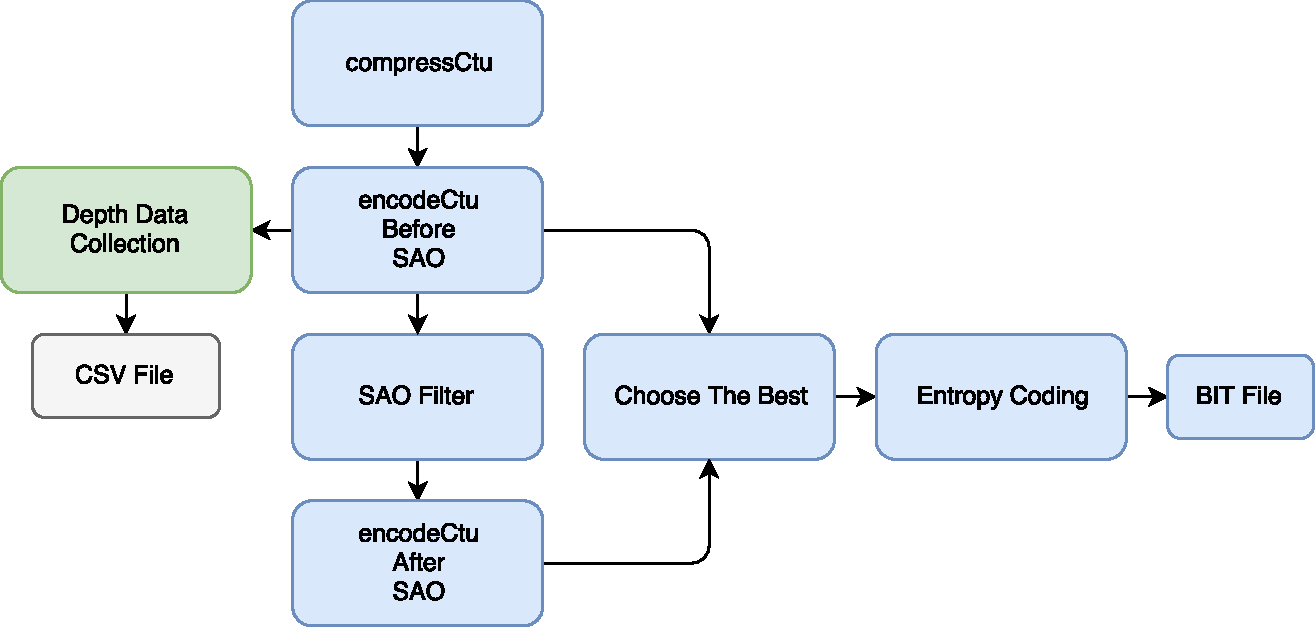
\includegraphics[width=\textwidth,height=\textheight,keepaspectratio]{Figures/thesis-data-collecting-diagram.pdf}
    \caption[Data collecting diagram]{Data collecting diagram.}
    \label{fig:data-collection-diagram}
\end{figure}
\begin{figure}
    \centering
    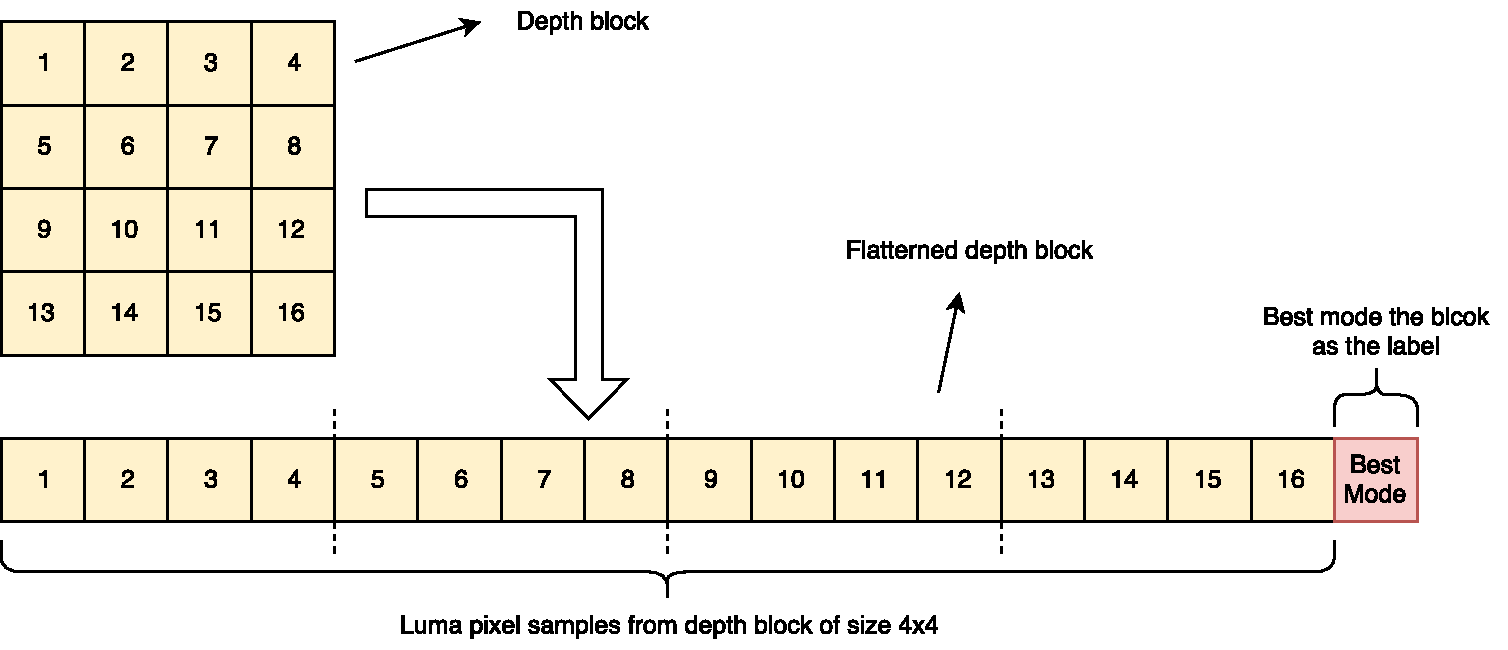
\includegraphics[width=\textwidth,height=\textheight,keepaspectratio]{Figures/flattern-pixels-into-single-line.pdf}
    \caption[Flattern Luma samples into one line and append best mode at the end]{Flattern Luma samples into one line and append best mode at the end.}
    \label{fig:flattern-data-into-one-dimension}
\end{figure}
During the data collecting process, only Luma samples in depth blocks
are used since we are trying to
reduce the computational complexity of DMM1.
Moreover, as shown in Figure~\ref{fig:flattern-data-into-one-dimension} 
on page~\pageref{fig:flattern-data-into-one-dimension},
the Luma samples are flattened from rectangle CU blocks into
a single row which will be subsequently written into associated CSV file.

The detailed implementation for the module of \emph{depth data collection}
is shown in Algorithm~\ref{algo:collect-data} 
on page~\pageref{algo:collect-data}.
\begin{algorithm}[!t]
    \SetKwData{pcCU}{pcCU}
    \SetKwData{Left}{left}
    \SetKwData{uiAbsPartIdx}{uiAbsPartIdx}
    \SetKwData{uiDepth}{uiDepth}
    \SetKwData{DISFlag}{DISFlag}
    \SetKwData{iPartNum}{iPartNum}
    \SetKwData{sizeOfNByN}{sizeOfNByN}
    \SetKwData{maxCUWidth}{maxCUWidth}
    \SetKwData{pcPic}{pcPic}
    \SetKwData{pcSlice}{pcSlice}
    \SetKwData{pOrg}{pOrg}
    \SetKwData{iStride}{iStride}
    \SetKwData{uiCuSize}{uiCuSize}
    \SetKwData{pOrgPel}{pOrgPel}
    \SetKwData{sizeOfSubBlk}{sizeOfSubBlk}
    \SetKwData{uiTPelY}{uiTPelY}
    \SetKwData{uiLPelX}{uiLPelX}
    \SetKwData{yStartPos}{yStartPos}
    \SetKwData{yEndPos}{yEndPos}
    \SetKwData{xStartPos}{xStartPos}
    \SetKwData{xEndPos}{xEndPos}
    \SetKwData{iDir}{iDir}
    \SetKwData{partitionMode}{partitionMode}
    \SetKwFunction{getCUSize}{getCUSize}
    \SetKwFunction{getSizeOfSubBlk}{getSizeOfSubBlk}
    \SetKwFunction{FindCompress}{FindCompress}
    \SetKwFunction{getIntraDir}{getIntraDir}
    \SetKwFunction{getPic}{getPic}
    \SetKwFunction{getSlice}{getSlice}
    \SetKwFunction{getAddr}{getAddr}
    \SetKwFunction{getStride}{getStride}
    \SetKwFunction{getYPelCU}{getYPelCU}
    \SetKwFunction{getPartitionSize}{getPartitionSize}
    \DontPrintSemicolon % Some LaTeX compilers require you to use \dontprintsemicolon instead
    \KwIn{CU data structure \pcCU,
    absolute partition index of CU \uiAbsPartIdx,
    quad-tree depth \uiDepth}
    \KwOut{Flattened luma pixel values of each block together with
    the index of its best intra mode in each row of the output csv file}
    \Begin{
    \For{each CU in depth maps}{
    \uiCuSize$\leftarrow$\getCUSize{\pcCU, \uiDepth}\;
    \pOrgPel$\leftarrow$\getYPelCU{\pcCU}\;
    \If{\DISFlag $\equiv 0$}{
    %  \partitionMode$\leftarrow$ \getPartitionSize{$Im[i,j-1]$}\;
    \partitionMode$\leftarrow$\getPartitionSize{\pcCU, \uiAbsPartIdx}\;

    \eIf{\partitionMode $\equiv$ \sizeOfNByN}{
    \iPartNum$\leftarrow 4$\;
    }{
    \iPartNum$\leftarrow 1$\;
    }

    \For{$j\leftarrow 0$ \KwTo \iPartNum}{
    $iDir[j]$ $\leftarrow$ \getIntraDir{\pcCU, \uiAbsPartIdx}\;
    }
    \eIf{\iPartNum $\equiv 1$}{
    %      \tcc{collect luma values and the best mode for a single block}
    Create a new csv file, append the value of \uiDepth at the end of the name of the new csv file\;
    \For{$y\leftarrow 0$ \KwTo \uiCuSize}{
    \For{$x\leftarrow 0$ \KwTo \uiCuSize}{
    Write $pOrgPel[x]$ into $row_m$ in csv file\;
    }
    \pOrgPel $\leftarrow$ \pOrgPel + \iStride\;
    }
    Write $iDir[0]$ into the end of $row_m$ in the csv file\;
    }{
    %      \tcc{collect luma values and the best modes for each sub parts}
    Create a new csv file, append the value of (\uiDepth + $1$) at the end of the name of the new csv file\;
    \sizeOfSubBlk$\leftarrow$\getSizeOfSubBlk{\pcCU, \uiDepth}\;
    \For{$j\leftarrow 0$ \KwTo \iPartNum}{
    \uIf{$j\equiv0$}{
    \yStartPos $\leftarrow 0$
    \& \xStartPos $\leftarrow 0$
    \& \yEndPos $\leftarrow$ \sizeOfSubBlk\
    \& \xEndPos $\leftarrow$ \sizeOfSubBlk\;
    }
    \uElseIf{$j\equiv1$}{
    \yStartPos $\leftarrow 0$
    \& \xStartPos $\leftarrow$ \sizeOfSubBlk
    \& \yEndPos $\leftarrow$ \sizeOfSubBlk
    \& \xEndPos $\leftarrow \sizeOfSubBlk \times 2$\;
    }
    \uElseIf{$j\equiv2$}{
    \yStartPos $\leftarrow$ \sizeOfSubBlk
    \& \xStartPos $\leftarrow 0$
    \& \yEndPos $\leftarrow \sizeOfSubBlk \times 2$
    \& \xEndPos $\leftarrow$ \sizeOfSubBlk\;
    }
    \uElseIf{$j\equiv3$}{
    \yStartPos $\leftarrow$ \sizeOfSubBlk
    \& \xStartPos $\leftarrow$ \sizeOfSubBlk
    \& \yEndPos $\leftarrow \sizeOfSubBlk \times 2$
    \& \xEndPos $\leftarrow \sizeOfSubBlk \times 2$\;
    }
    }
    \For{$y\leftarrow$ \yStartPos \KwTo \yEndPos}{
    \For{$x\leftarrow$ \xStartPos \KwTo \xEndPos}{
    %   \For{$y\leftarrow 0$ \KwTo \yEndPos}{
    %        \For{$x\leftarrow 0$ \KwTo \xEndPos}{
    Write $pOrgPel[x]$ into $row_m$ in the csv file\;
    }
    \pOrgPel $\leftarrow$ \pOrgPel+ \iStride\;
    }
    Write $iDir[j]$ into the end of $row_m$ in the csv file\;
    }}}}
 \caption{Collect data}
 \label{algo:collect-data}
\end{algorithm}
The inputs to the data collecting workflow are exactly the inputs to
the module of \emph{encodeCtu}, namely the CU data structure,
the absolute partition index and the corresponding quad-tree depth.
Firstly, the partition mode of the CU is obtained which can further indicate
the partition number to either be one or four.
After that, based on the partition number, the best modes for blocks
are stored into an four dimensional array of integer values within the range
from 0 (inclusive) to 36 (inclusive).
If the partition number is equal to one, which means the current CU has not
been split and it has its own best mode.
The luma pixel samples of this block are collected into a single row in the
CSV file.
In the end of the same row, the best mode of the CU is signaled.
If the partition number is equal to four, which means the current CU has been
split to form four smaller sub-blocks with each sub-block has its
own best mode.
The luma samples for each sub-block are collected into four different rows
in the CSV file with the last value in each row to be the best mode for each
sub-block.
HTM16.2~\parencite{RN214} is used in this work, which is the newest
version of the reference software of 3D-HEVC\@.
Considering we are focusing on the intra prediction,
All-Intra configuration is used.

\section{Data Visualization}\label{sec:data-visu}
Visualizing data is a good way for human to better understand
and memorize information. 
Complex patterns hidden in the data are easier to be discovered when they 
are aesthetically presented via the graphical format.
% We visualize the collected data to understand them
% more clearly.
The collected data are visualized with the hope of
discovering more information from them.
% They shall be sufficient to support the discussions which are
% ;Showing visualizations for four sets of 
% Due to the large quantity of the data from the visualization perspective,
% based on the observations.
Discussions based on the observations of the visualized blocks
are given, which convince us about the necessity of data 
pre-processing in Section~\ref{sec:data-preprocessing} before 
training the deep models.

\subsection{Visualized Data}\label{subsec:see-data-visu}
We have four sets of data which are from blocks of size
\(4\times4\), \(8\times8\), \(16\times16\) to \(32\times32\).
% However, only the part of the visualization for data of block 
% size \(8\\times8\) are presented in this section due to the 
% below considerations:
The intra prediction modes in 3D-HEVC include
DC mode, Planar mode, 33 angular modes, DMM1 and DMM4.
In this thesis, several indices are assigned to each mode:
0 for DC mode, 1 for Planar mode, {[2,34]} for 33 angular modes, 35
for DMM1 and 36 for DMM4.

After all the four sets of data have been visualized,
it is found that four corresponding sets of visualizations
give the same hints.
Besides, to avoid too much visualizations' occupation of the thesis,
only the visualizations of blocks of size $8\times8$
are shown.
There are totally 37 figures presented in this subsection,
from Figure~\ref{fig:size8_mode0}, Figure~\ref{fig:size8_mode1},
\ldots to Figure~\ref{fig:size8_mode36}.

\begin{figure}[H]

    \vspace*{1cm} % vertical separation
    
    \begin{minipage}{0.49\textwidth}
        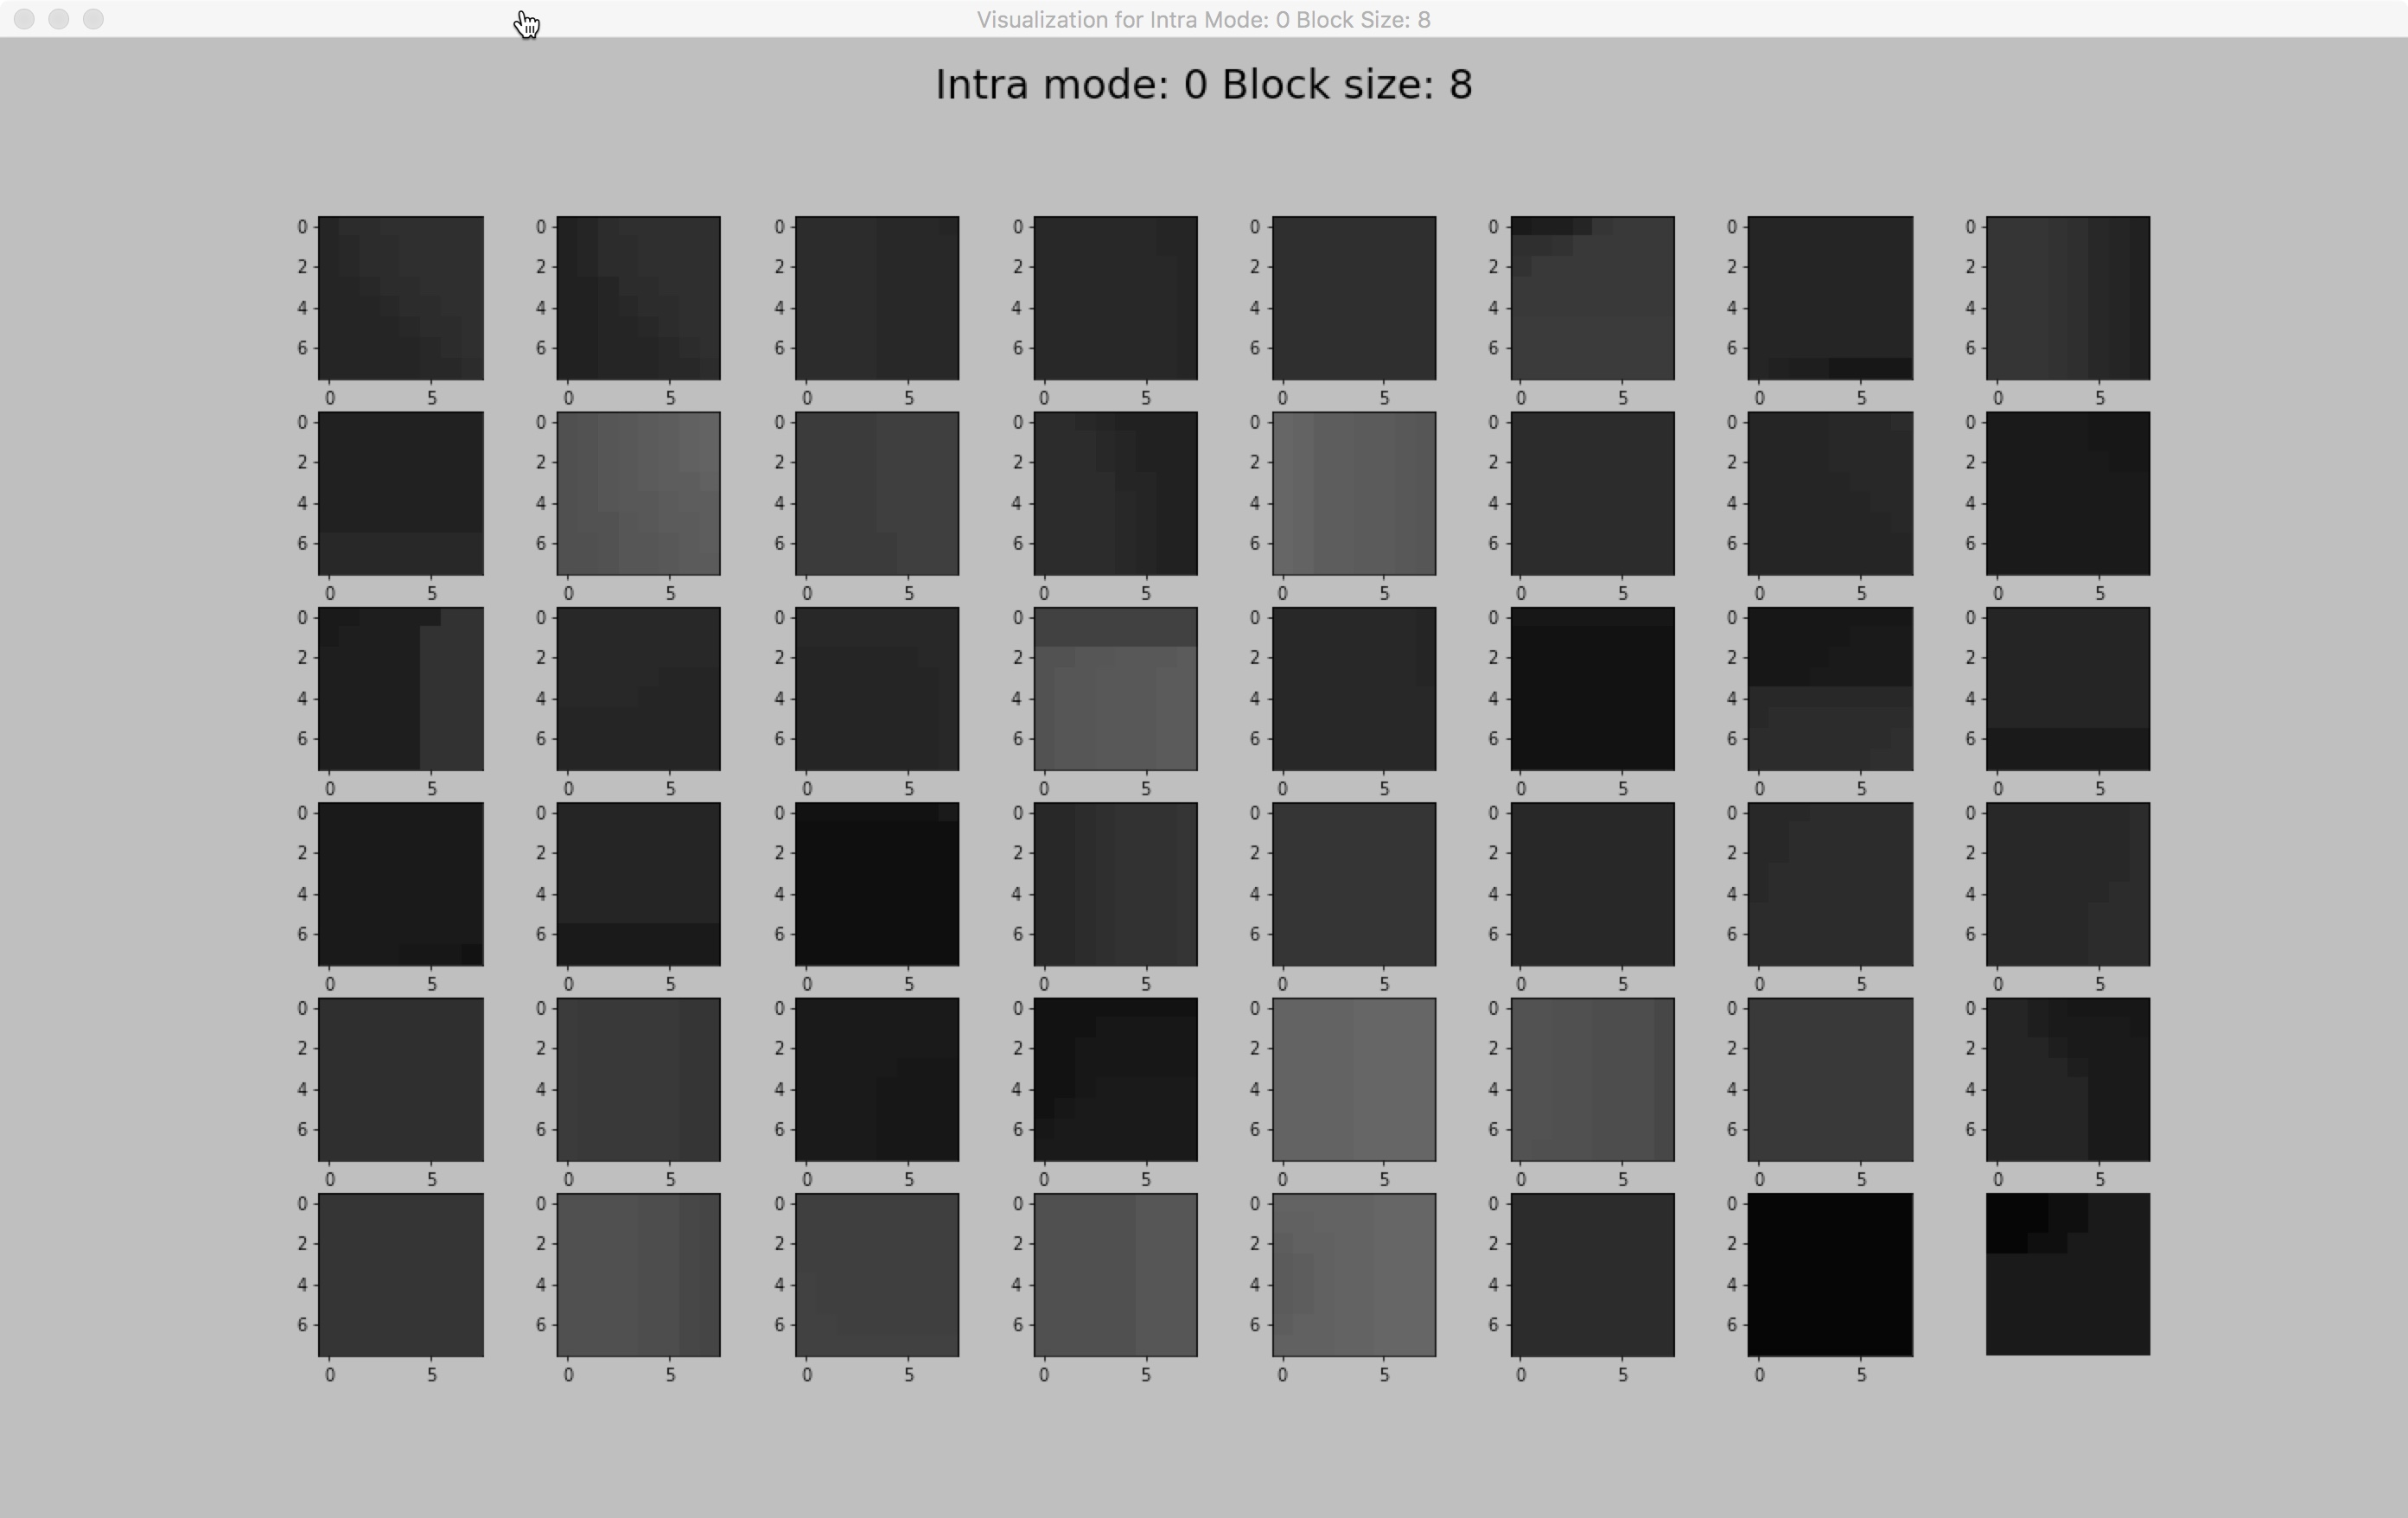
\includegraphics[width=\linewidth]{Figures/visu-size8x8/8-0}
        \caption[Intra mode 0]{intra mode 0.}
        \label{fig:size8_mode0}
    \end{minipage}
    \hspace{\fill} % note: no blank line here
    \begin{minipage}{0.49\textwidth}
        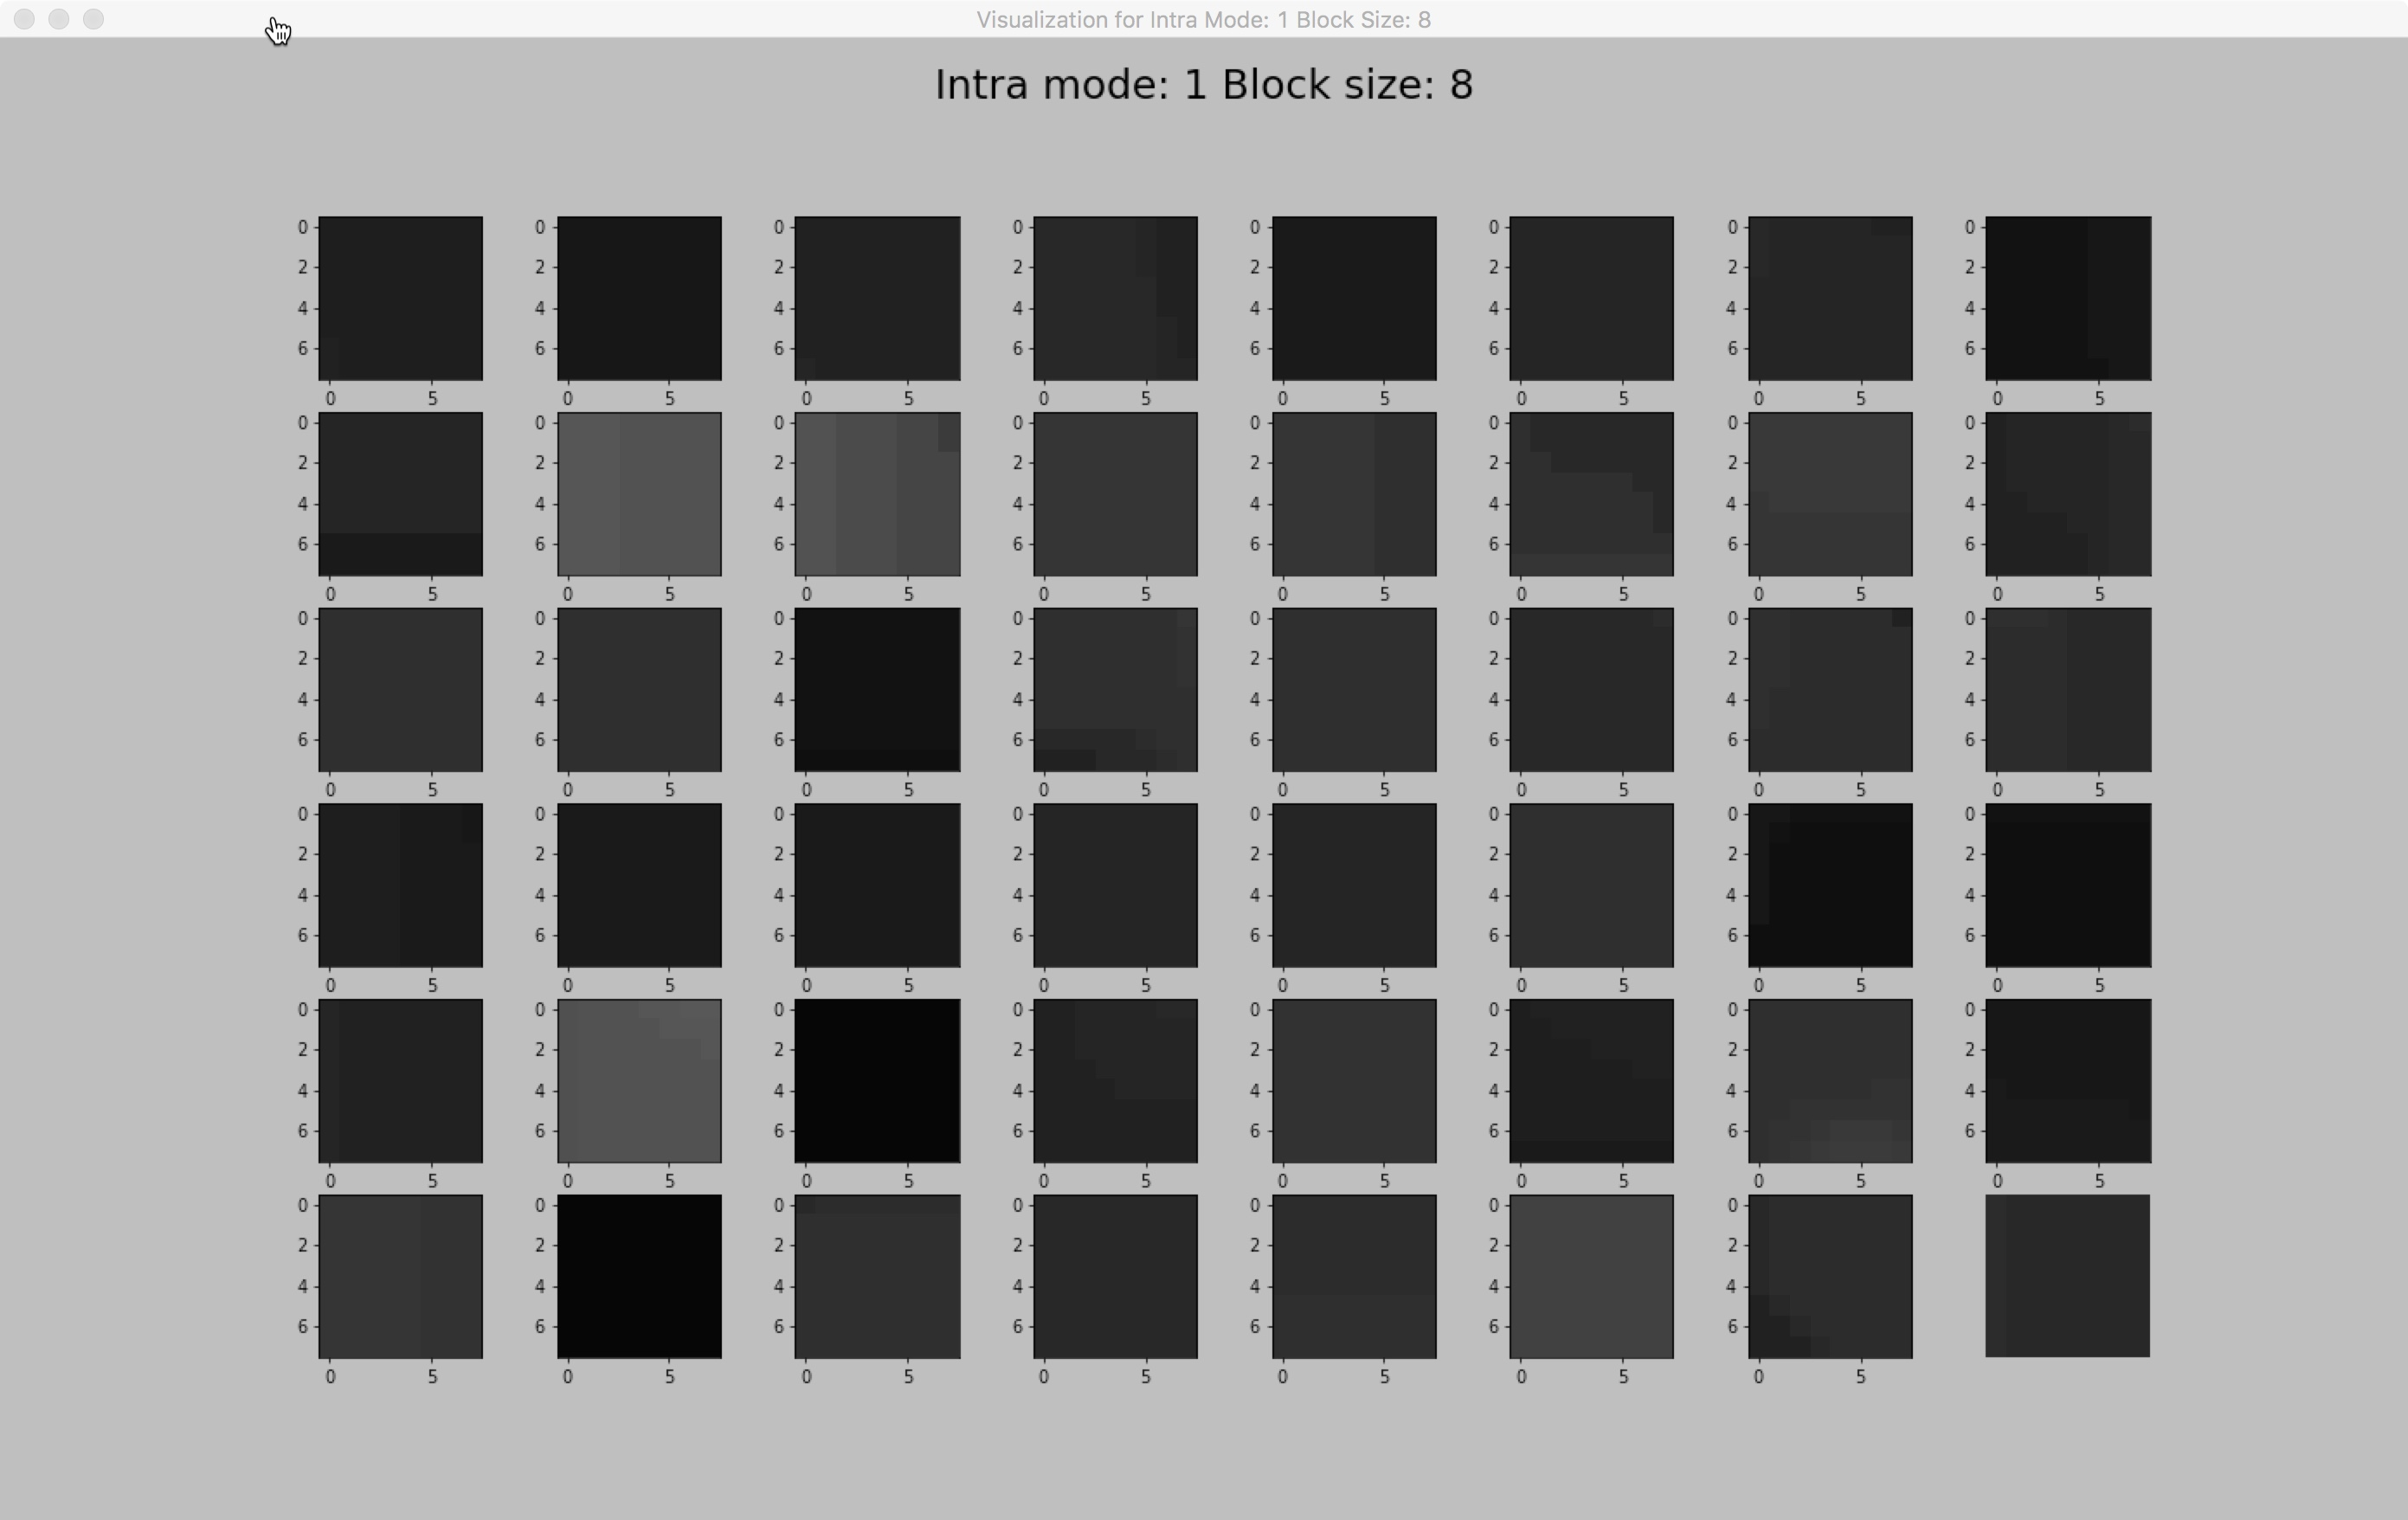
\includegraphics[width=\linewidth]{Figures/visu-size8x8/8-1}
        \caption[Intra mode 1]{intra mode 1.}
        \label{fig:size8_mode1}
    \end{minipage}
    
    \vspace*{1cm} % vertical separation

    \begin{minipage}{0.49\textwidth}
        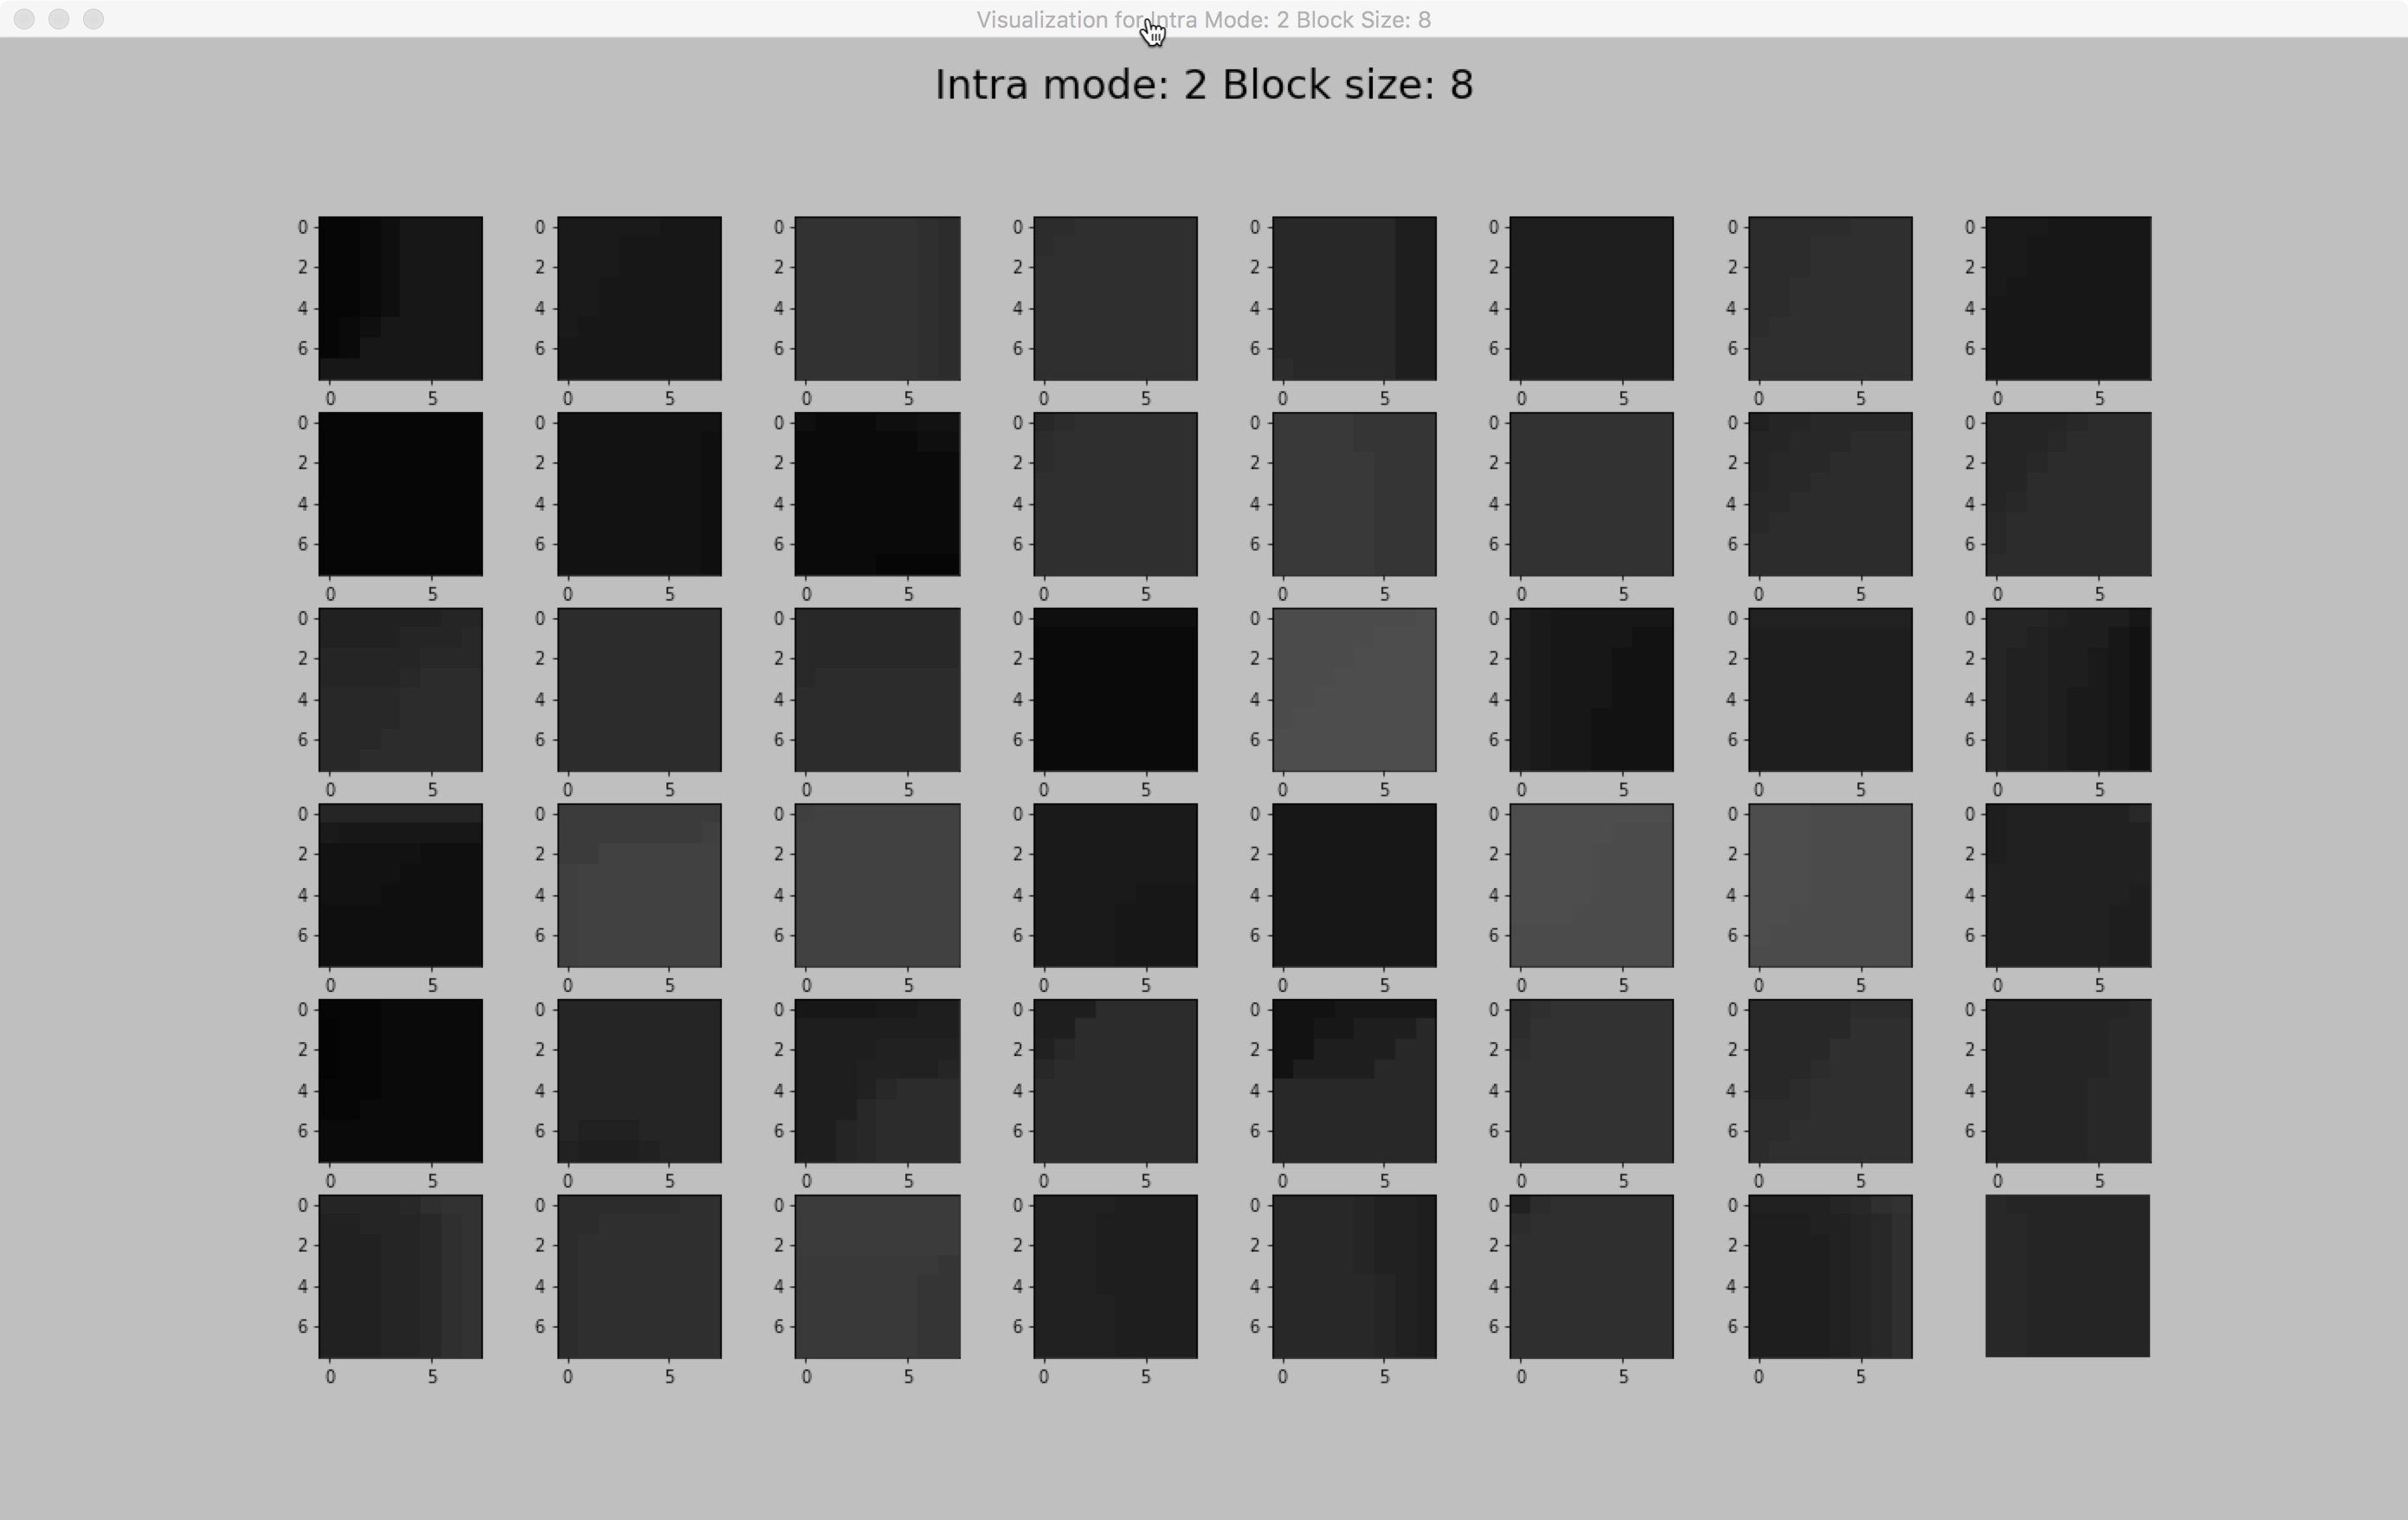
\includegraphics[width=\linewidth]{Figures/visu-size8x8/8-2.jpeg}
        \caption[Intra mode 2]{intra mode 2.}
        \label{fig:size8_mode2}
    \end{minipage}
    \hspace{\fill} % note: no blank line here
    \begin{minipage}{0.49\textwidth}
        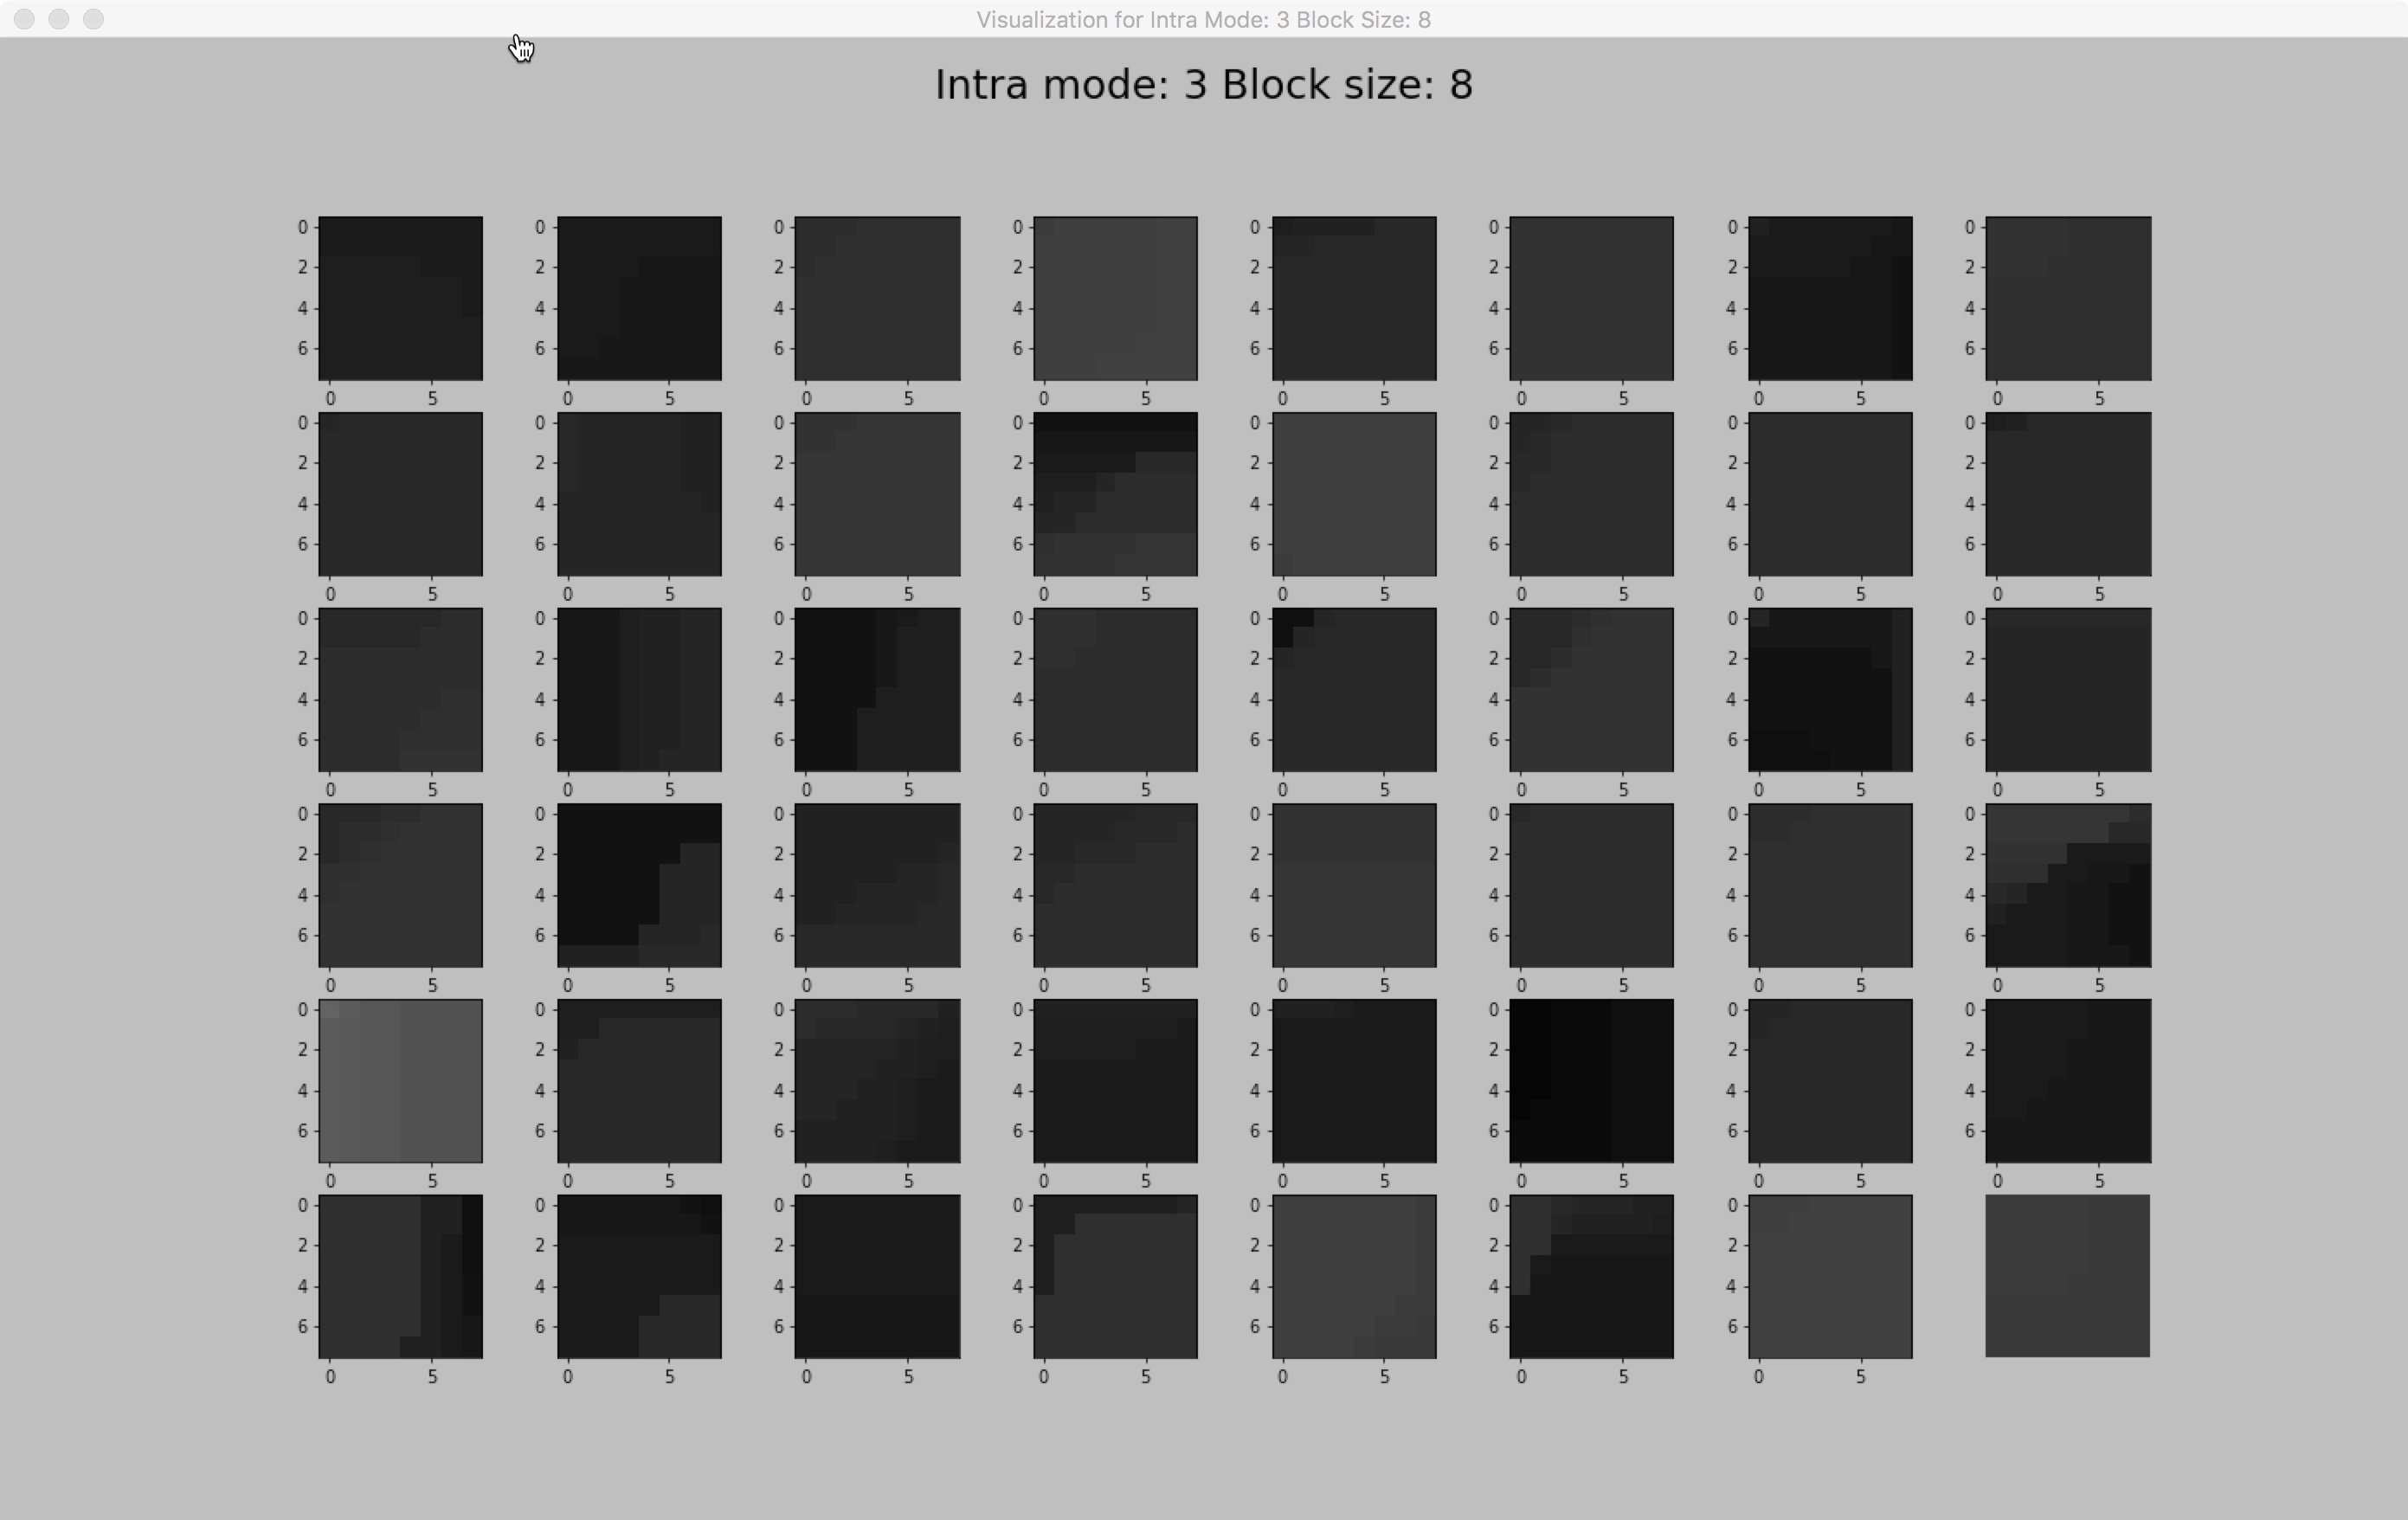
\includegraphics[width=\linewidth]{Figures/visu-size8x8/8-3}
        \caption[Intra mode 3]{intra mode 3.}
        \label{fig:size8_mode3}
    \end{minipage}
\end{figure}

\begin{figure}[H]

    \vspace*{1cm} % vertical separation
    
    \begin{minipage}{0.49\textwidth}
        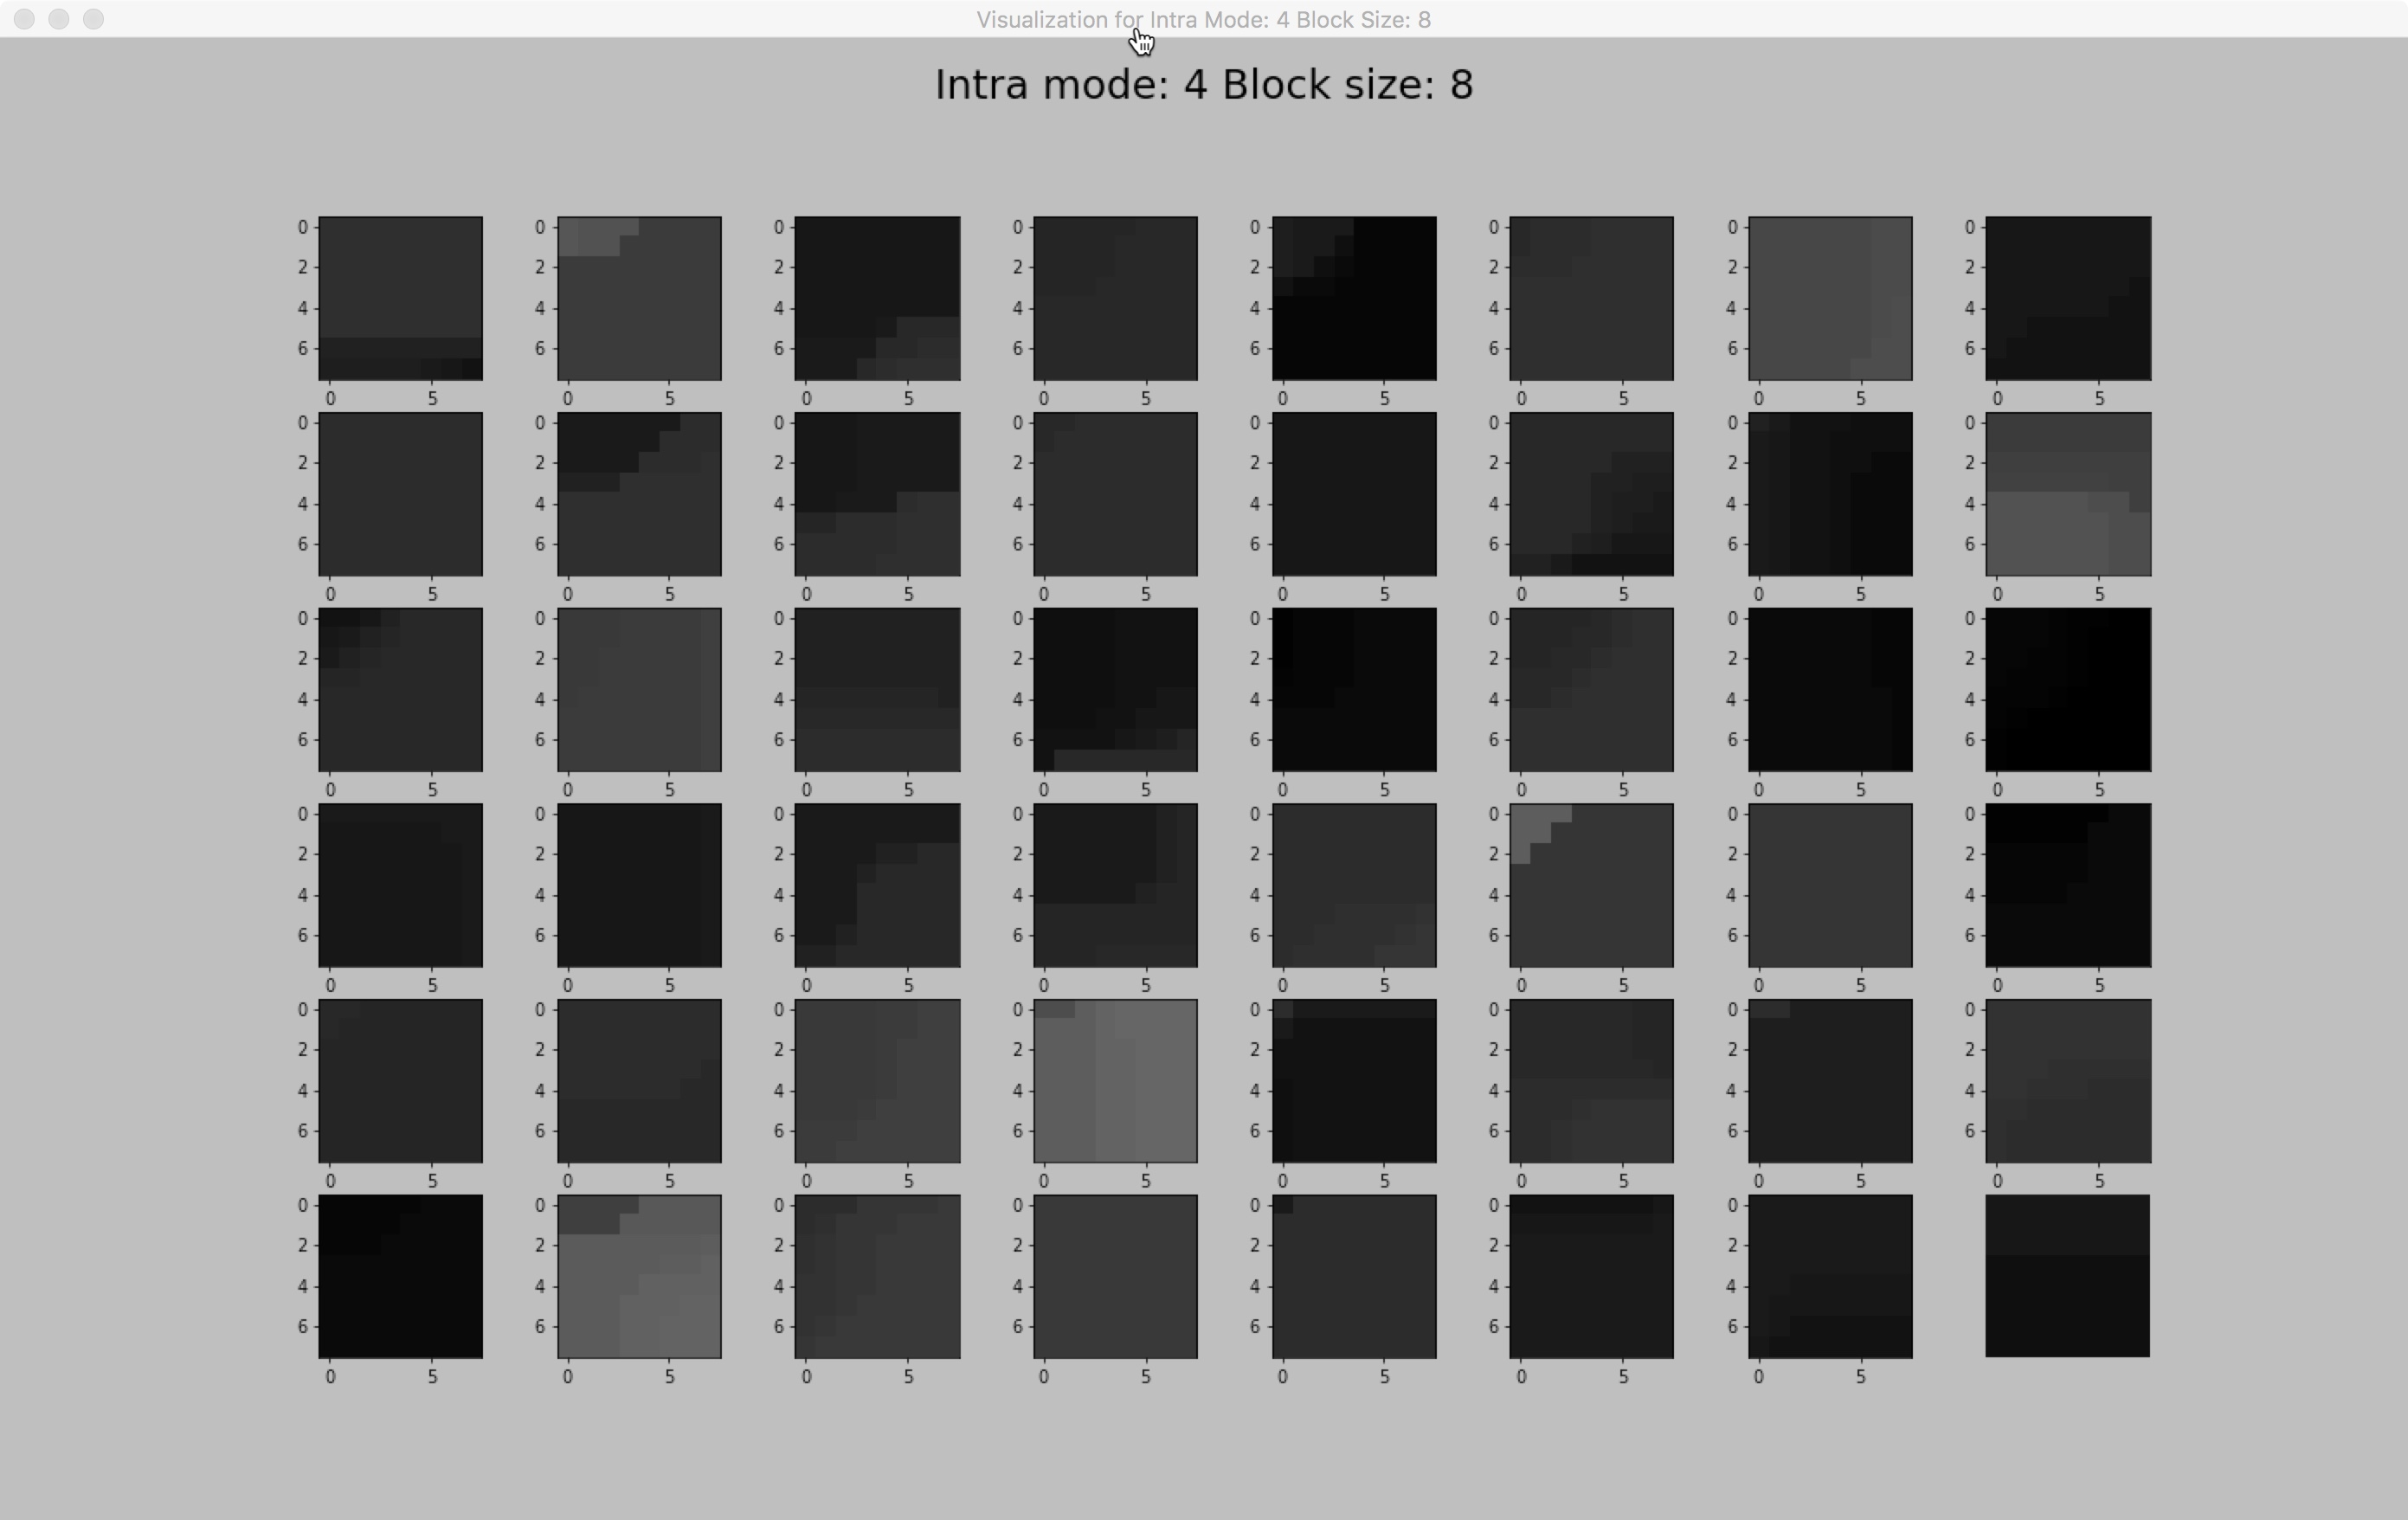
\includegraphics[width=\linewidth]{Figures/visu-size8x8/8-4}
        \caption[Intra mode 4]{intra mode 4.}
        \label{fig:size8_mode4}
    \end{minipage}
    \hspace{\fill} % note: no blank line here
    \begin{minipage}{0.49\textwidth}
        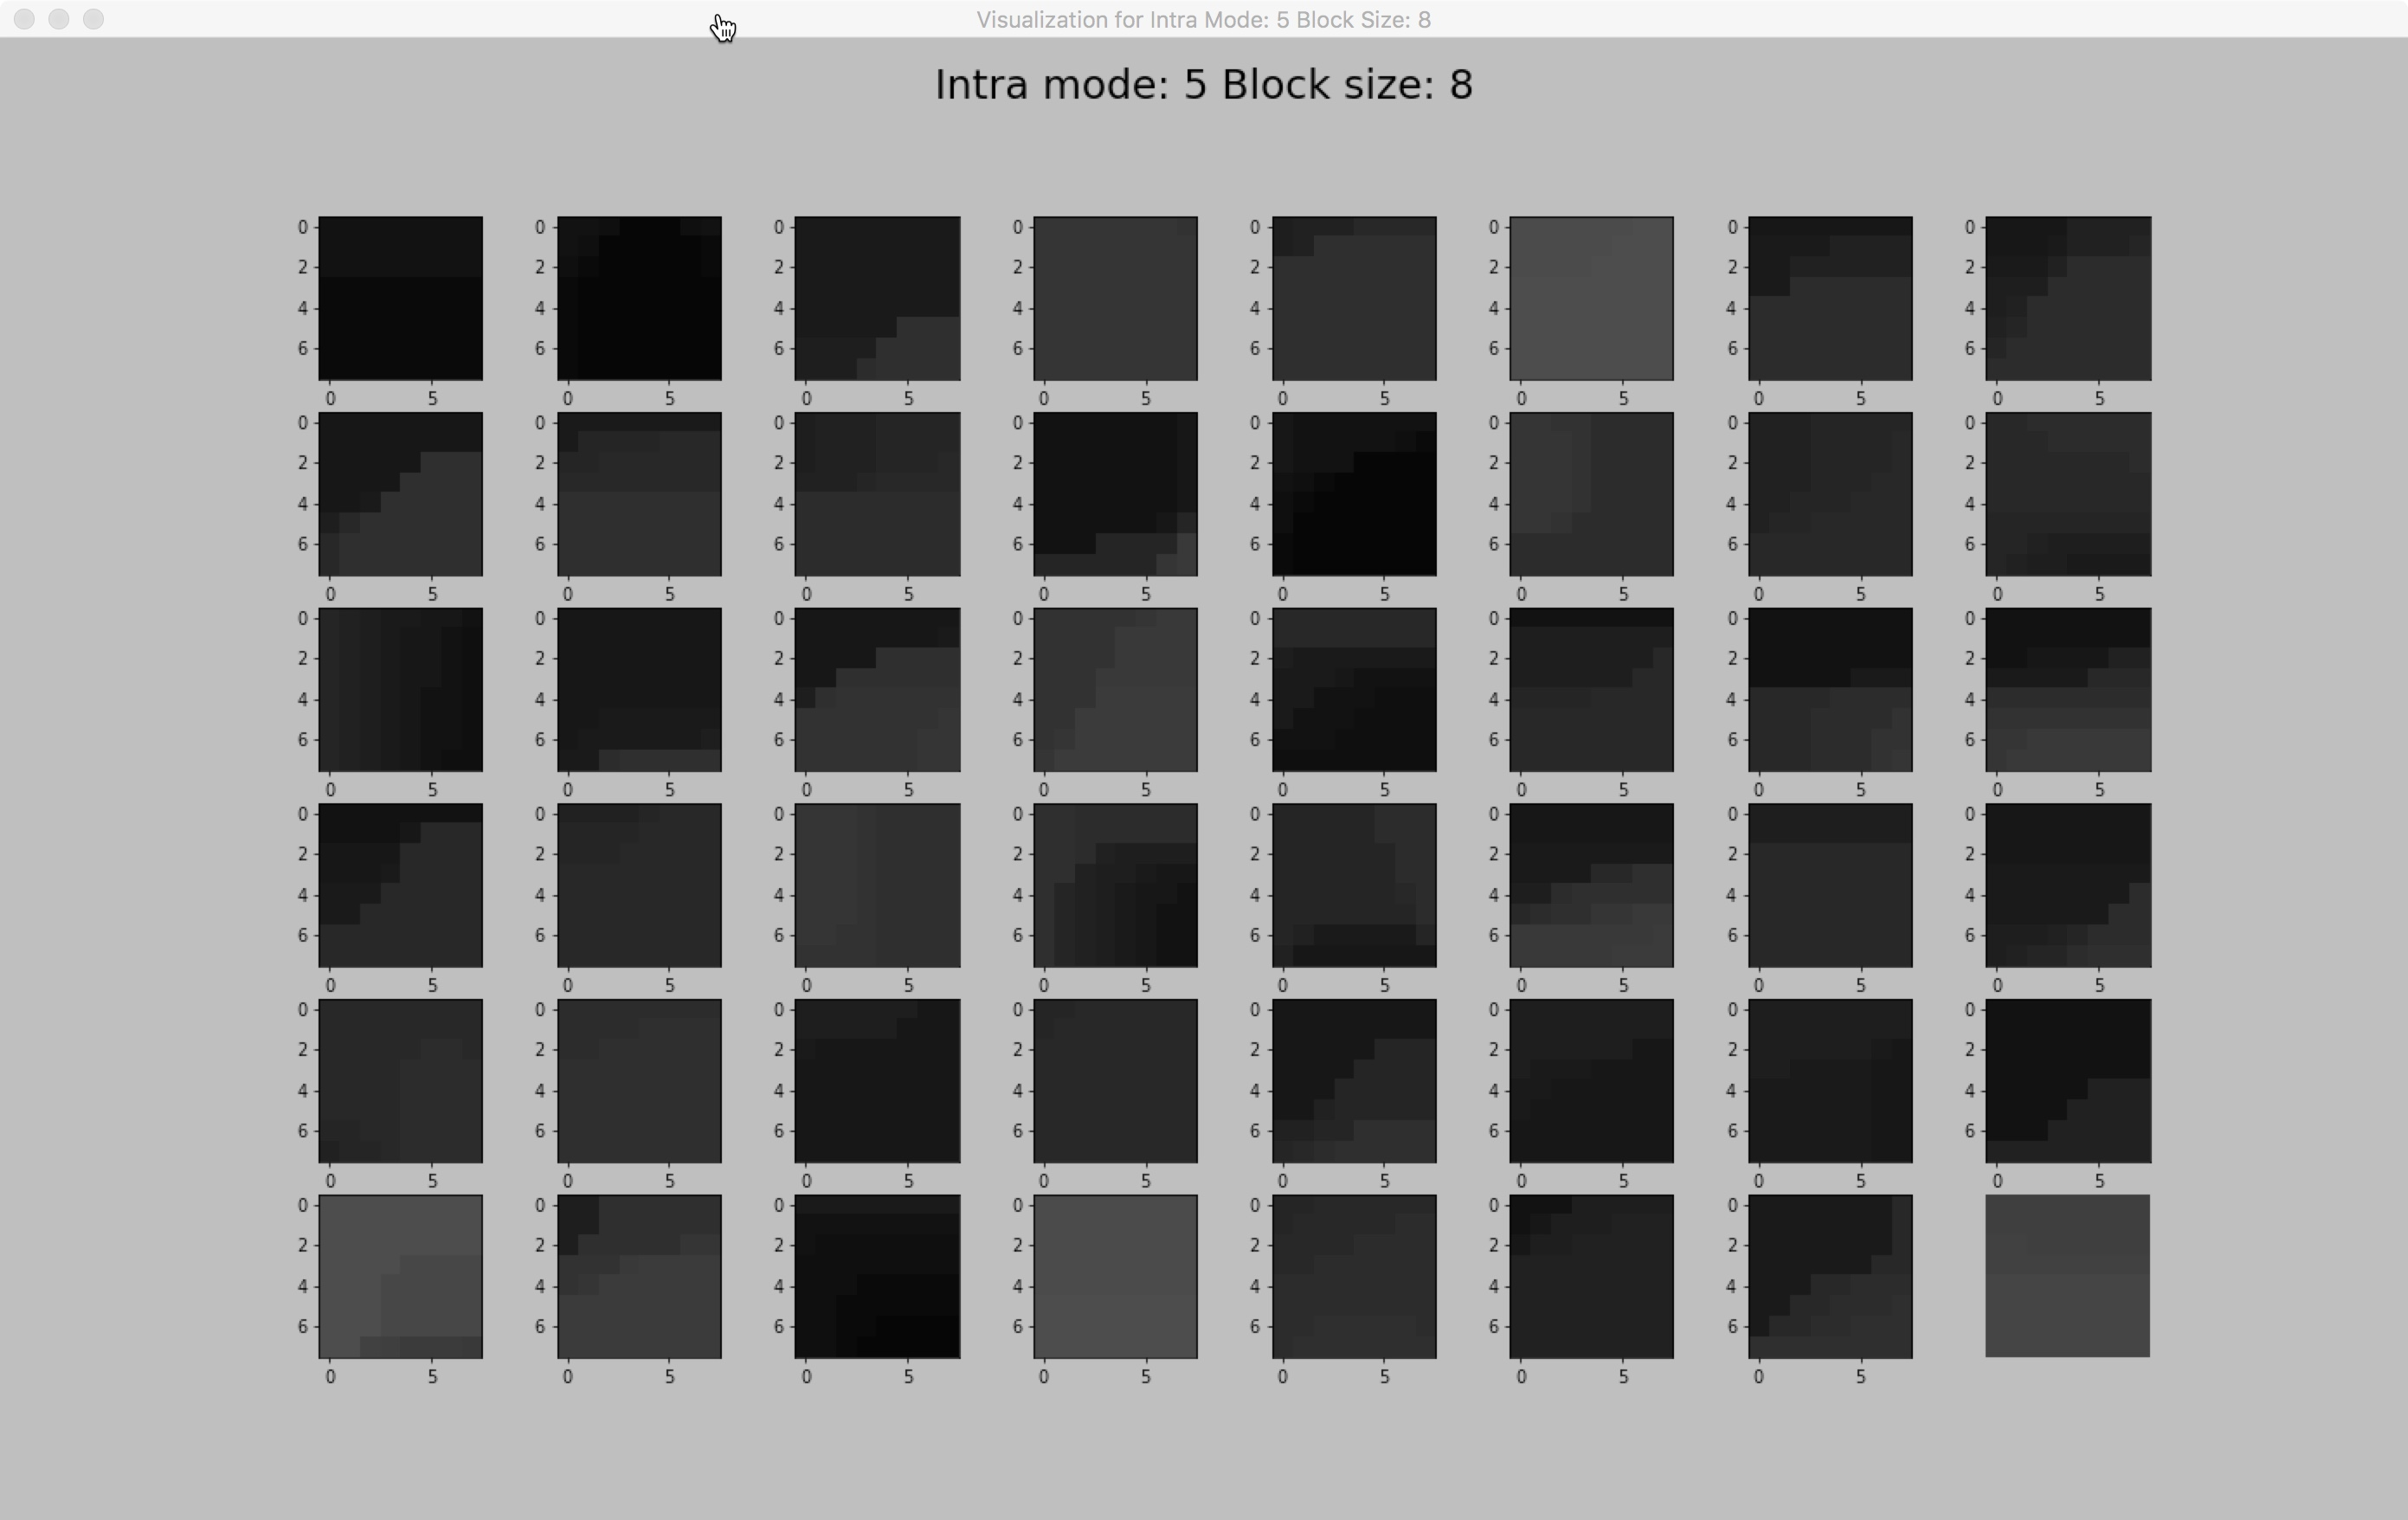
\includegraphics[width=\linewidth]{Figures/visu-size8x8/8-5}
        \caption[Intra mode 5]{intra mode 5.}
        \label{fig:size8_mode5}
    \end{minipage}

    \vspace*{1cm} % vertical separation

    \begin{minipage}{0.49\textwidth}
        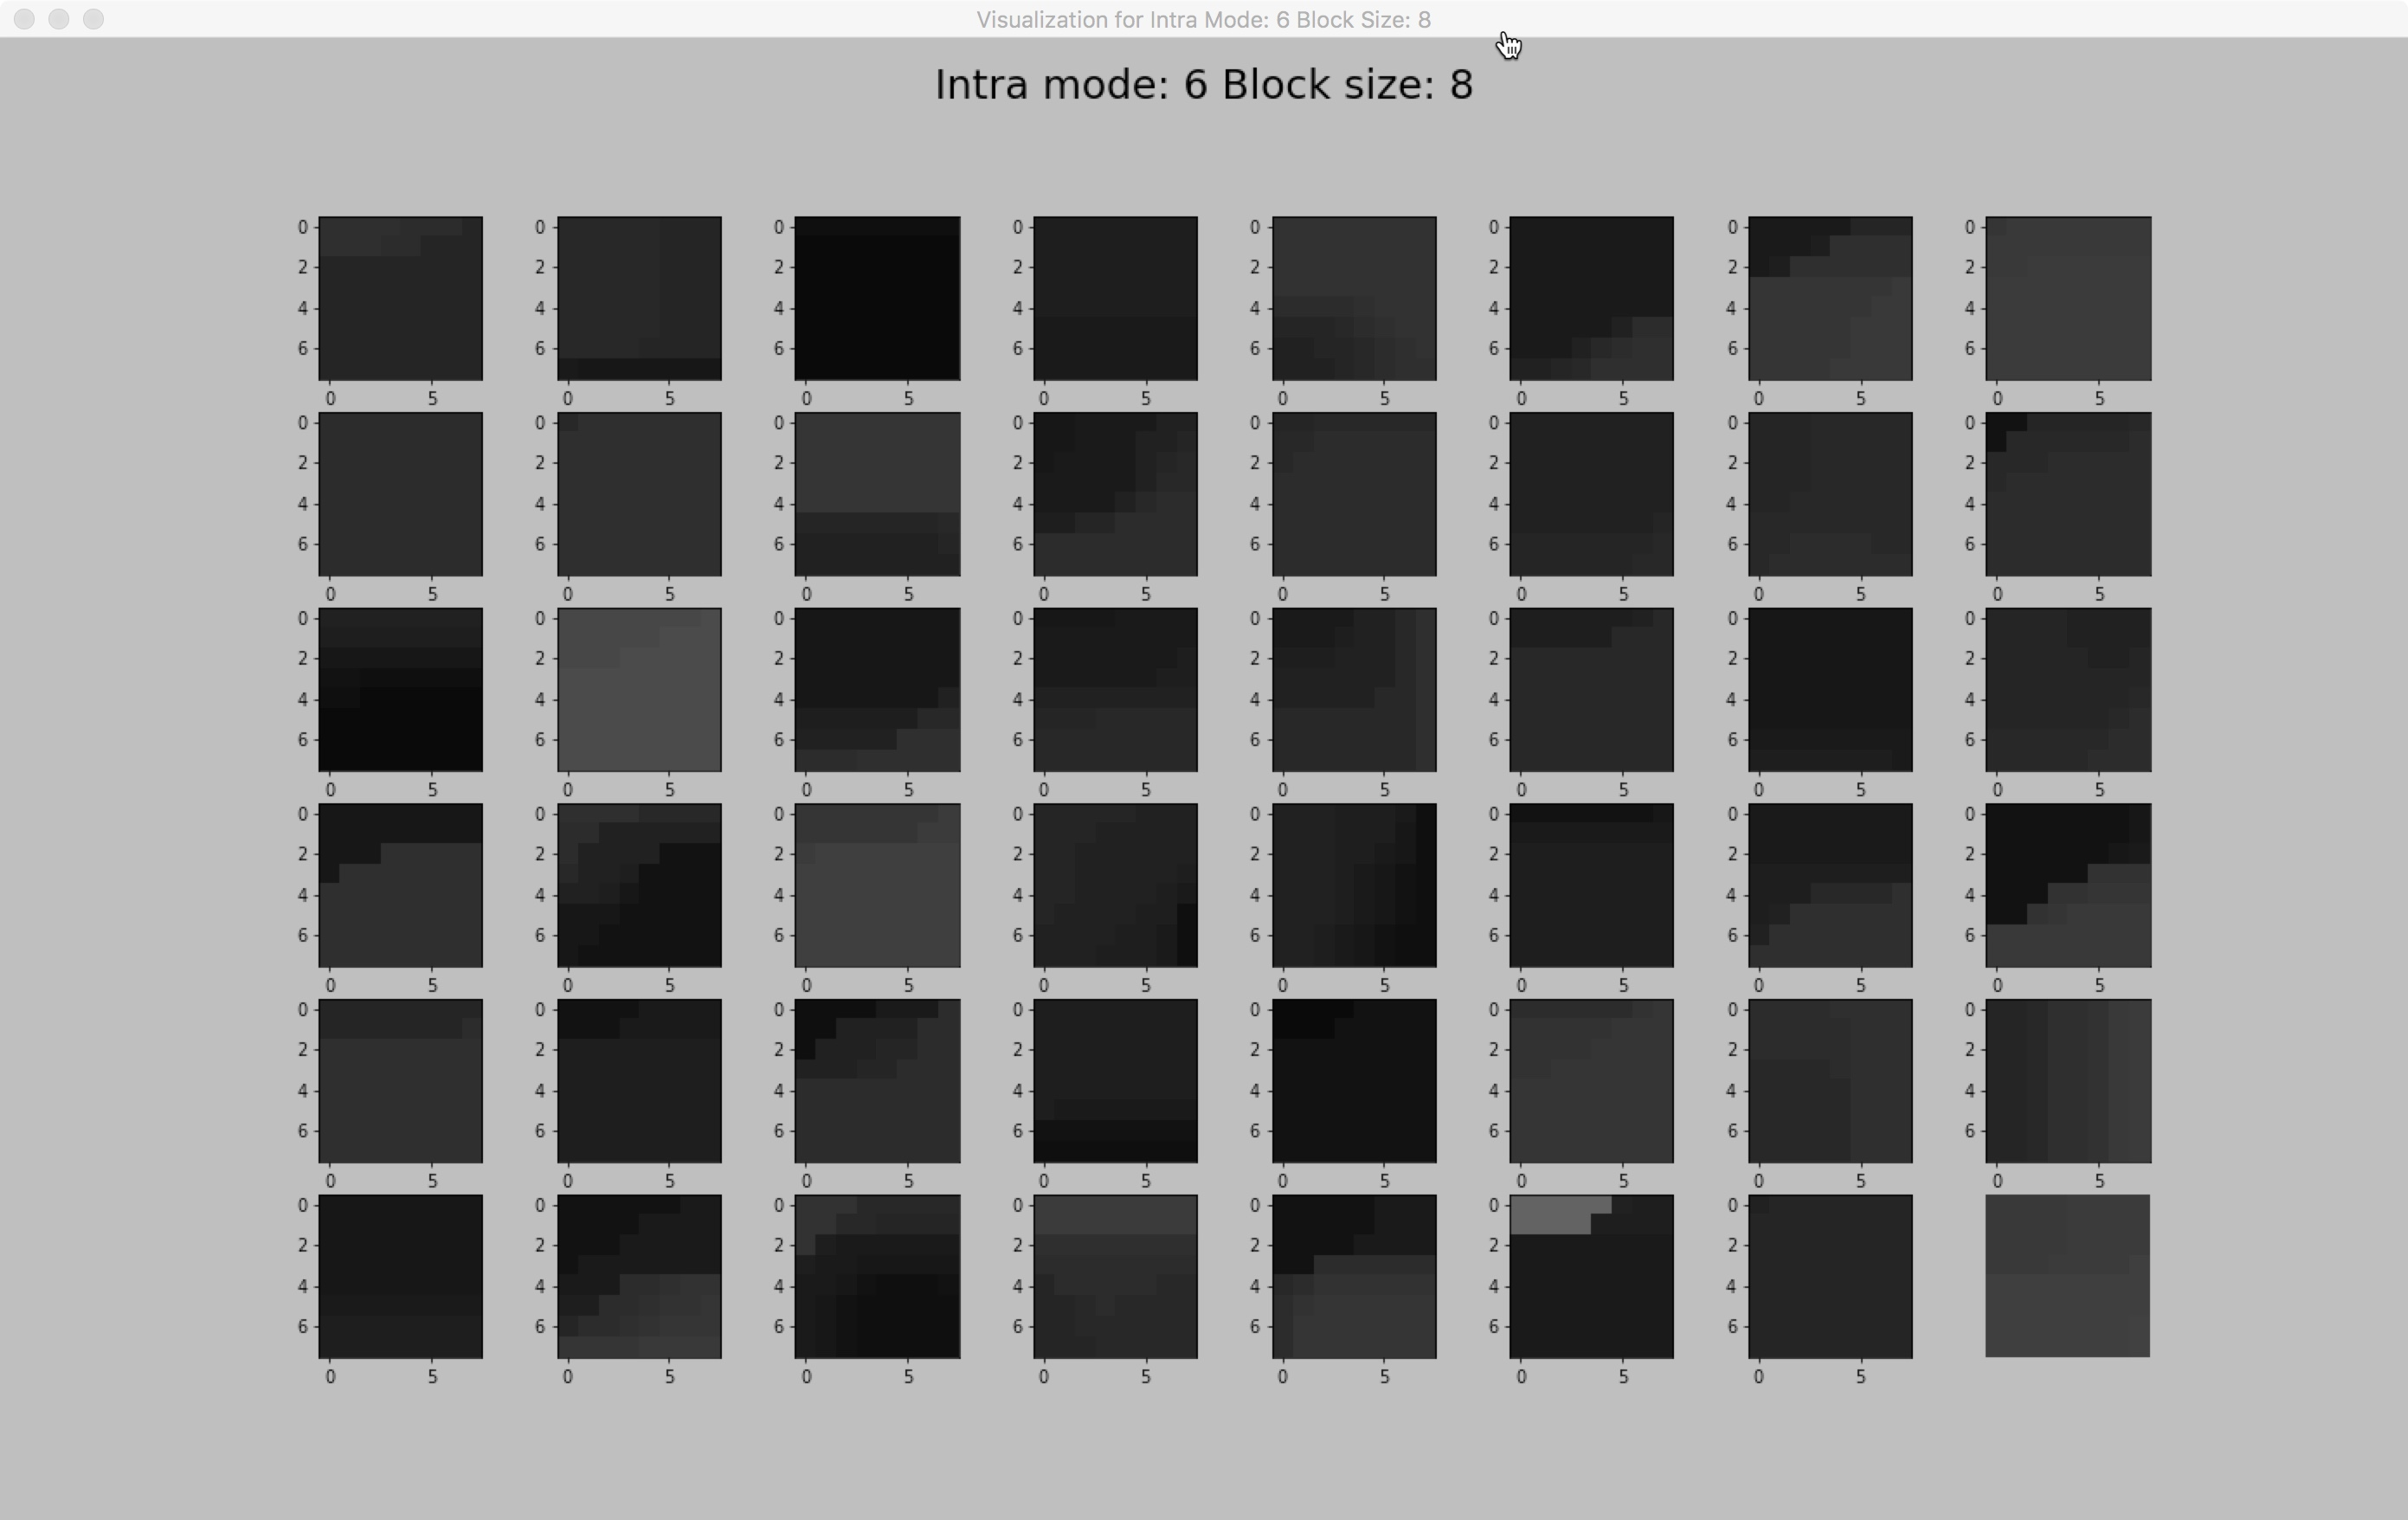
\includegraphics[width=\linewidth]{Figures/visu-size8x8/8-6}
        \caption[Intra mode 6]{intra mode 6.}
        \label{fig:size8_mode6}
    \end{minipage}
    \hspace{\fill} % note: no blank line here
    \begin{minipage}{0.49\textwidth}
        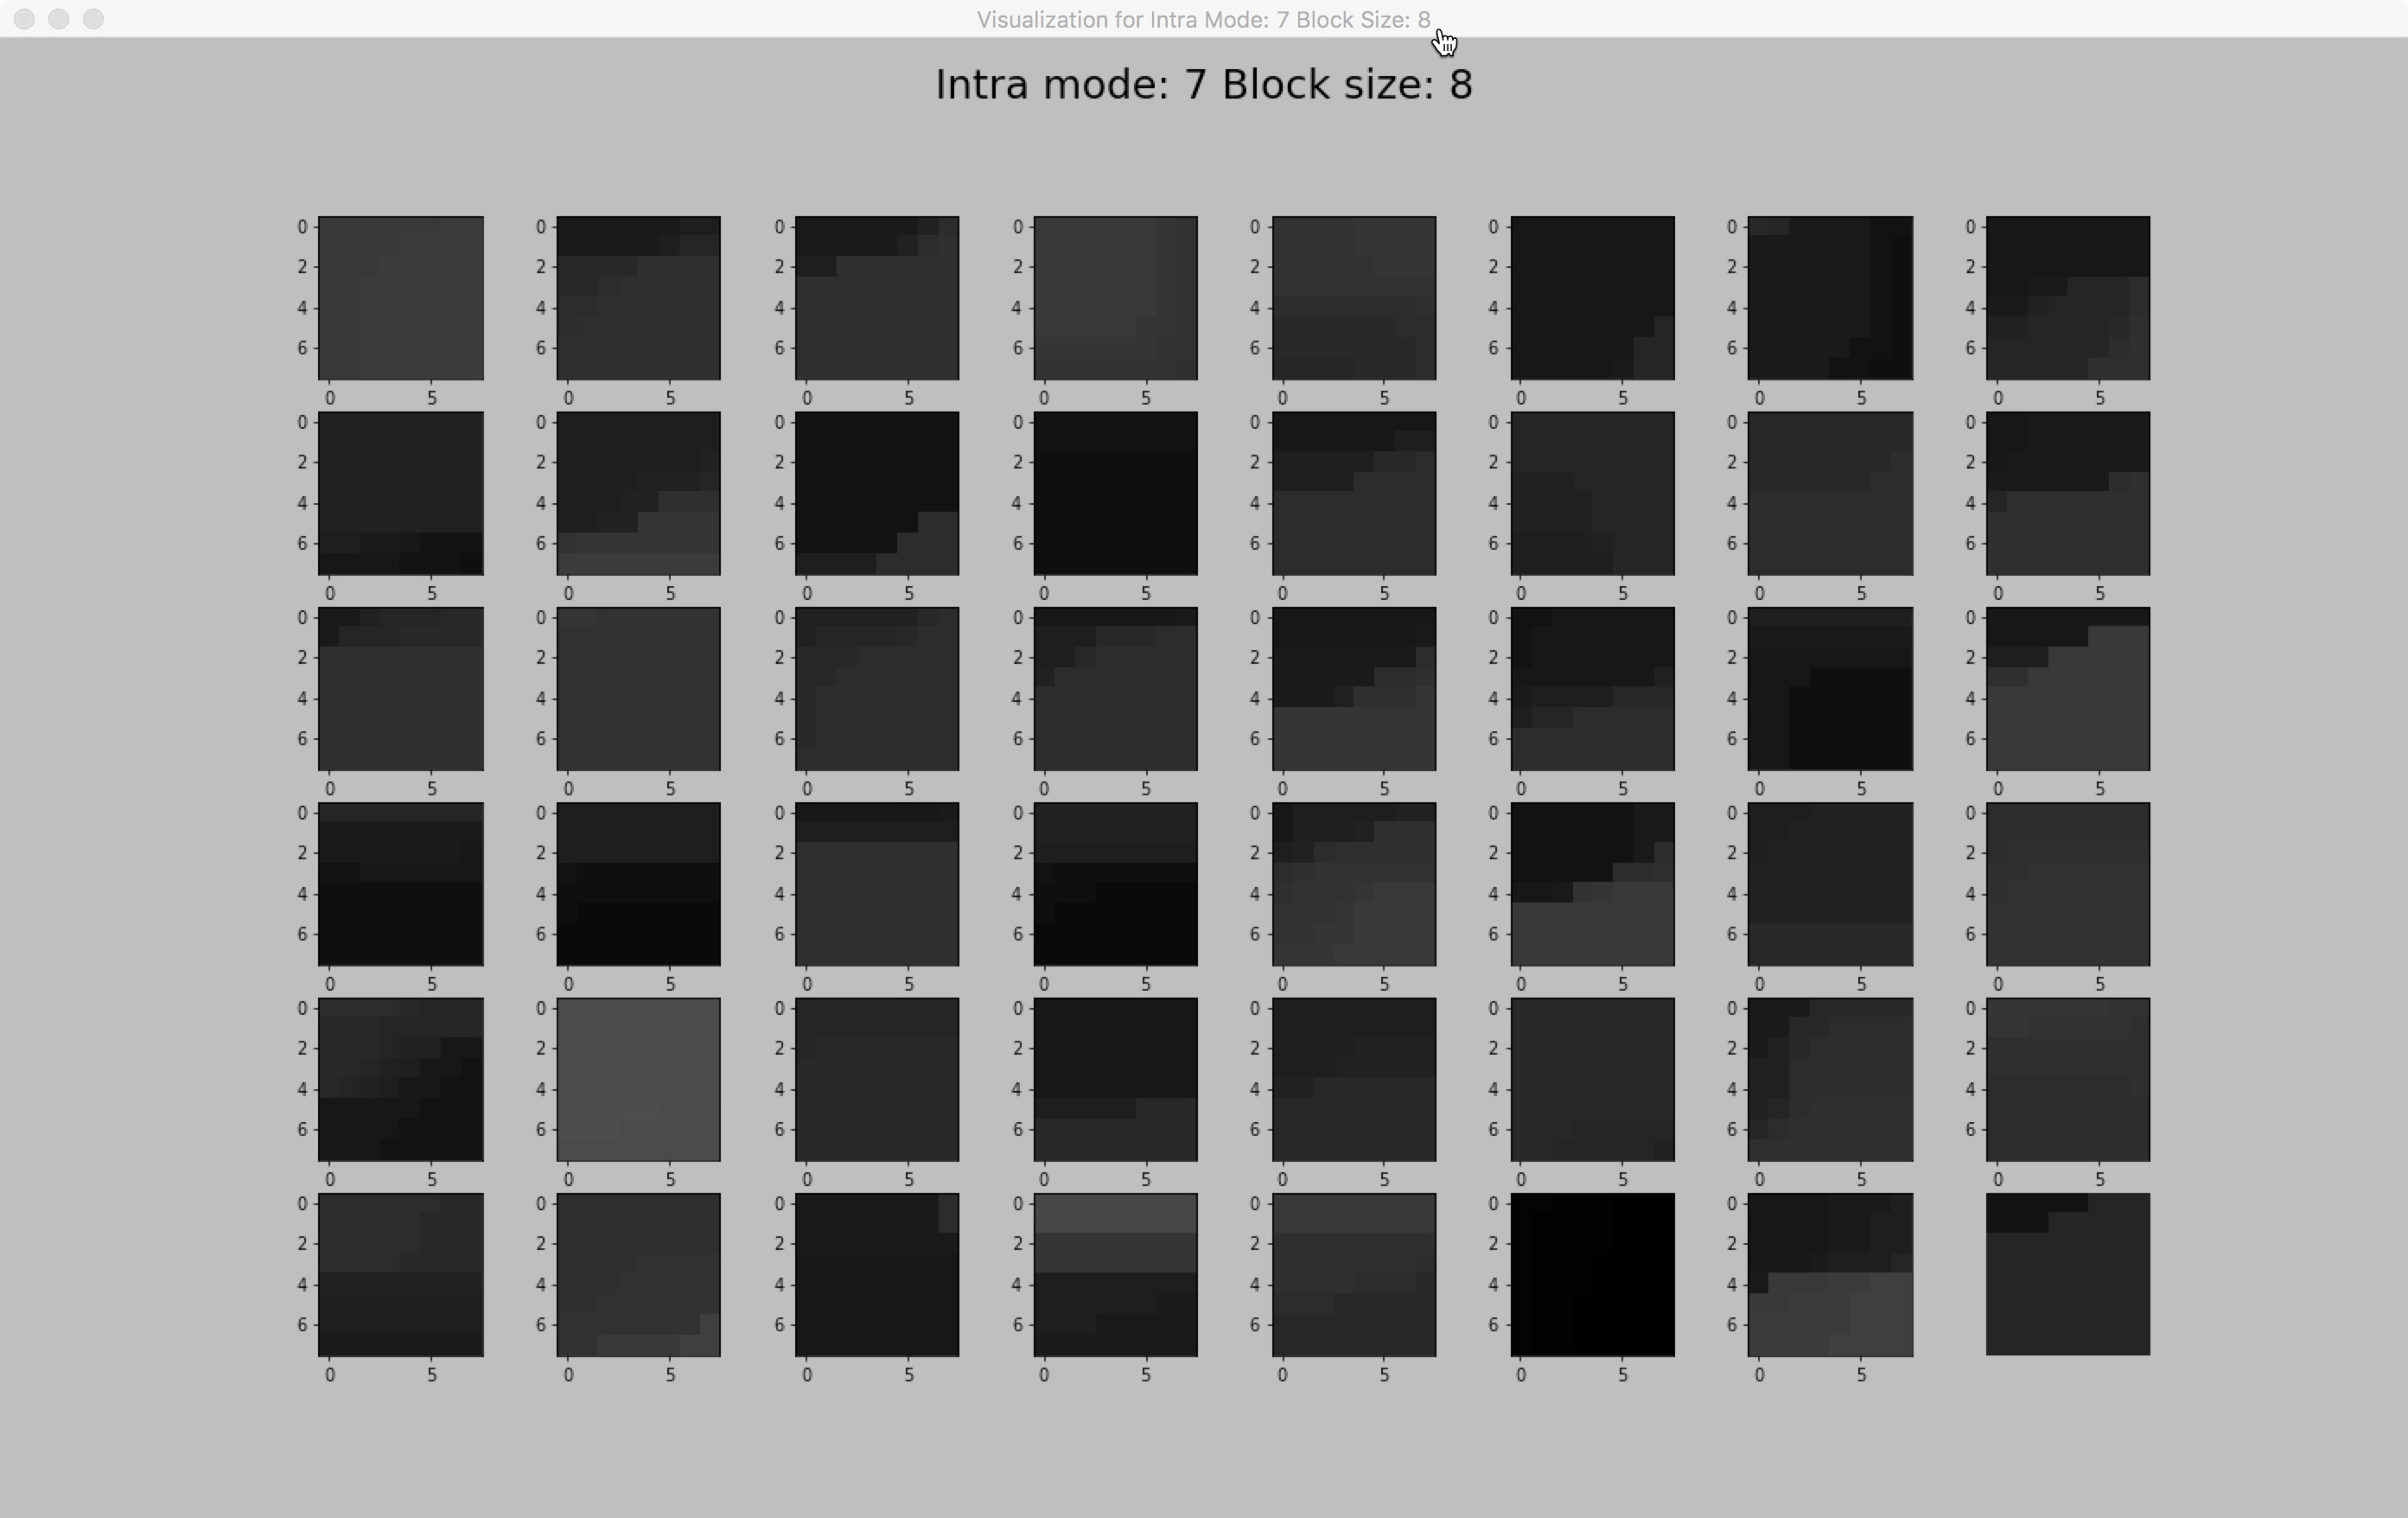
\includegraphics[width=\linewidth]{Figures/visu-size8x8/8-7}
        \caption[Intra mode 7]{intra mode 7.}
        \label{fig:size8_mode7}
    \end{minipage}
    
    \vspace*{1cm} % vertical separation

    \begin{minipage}{0.49\textwidth}
        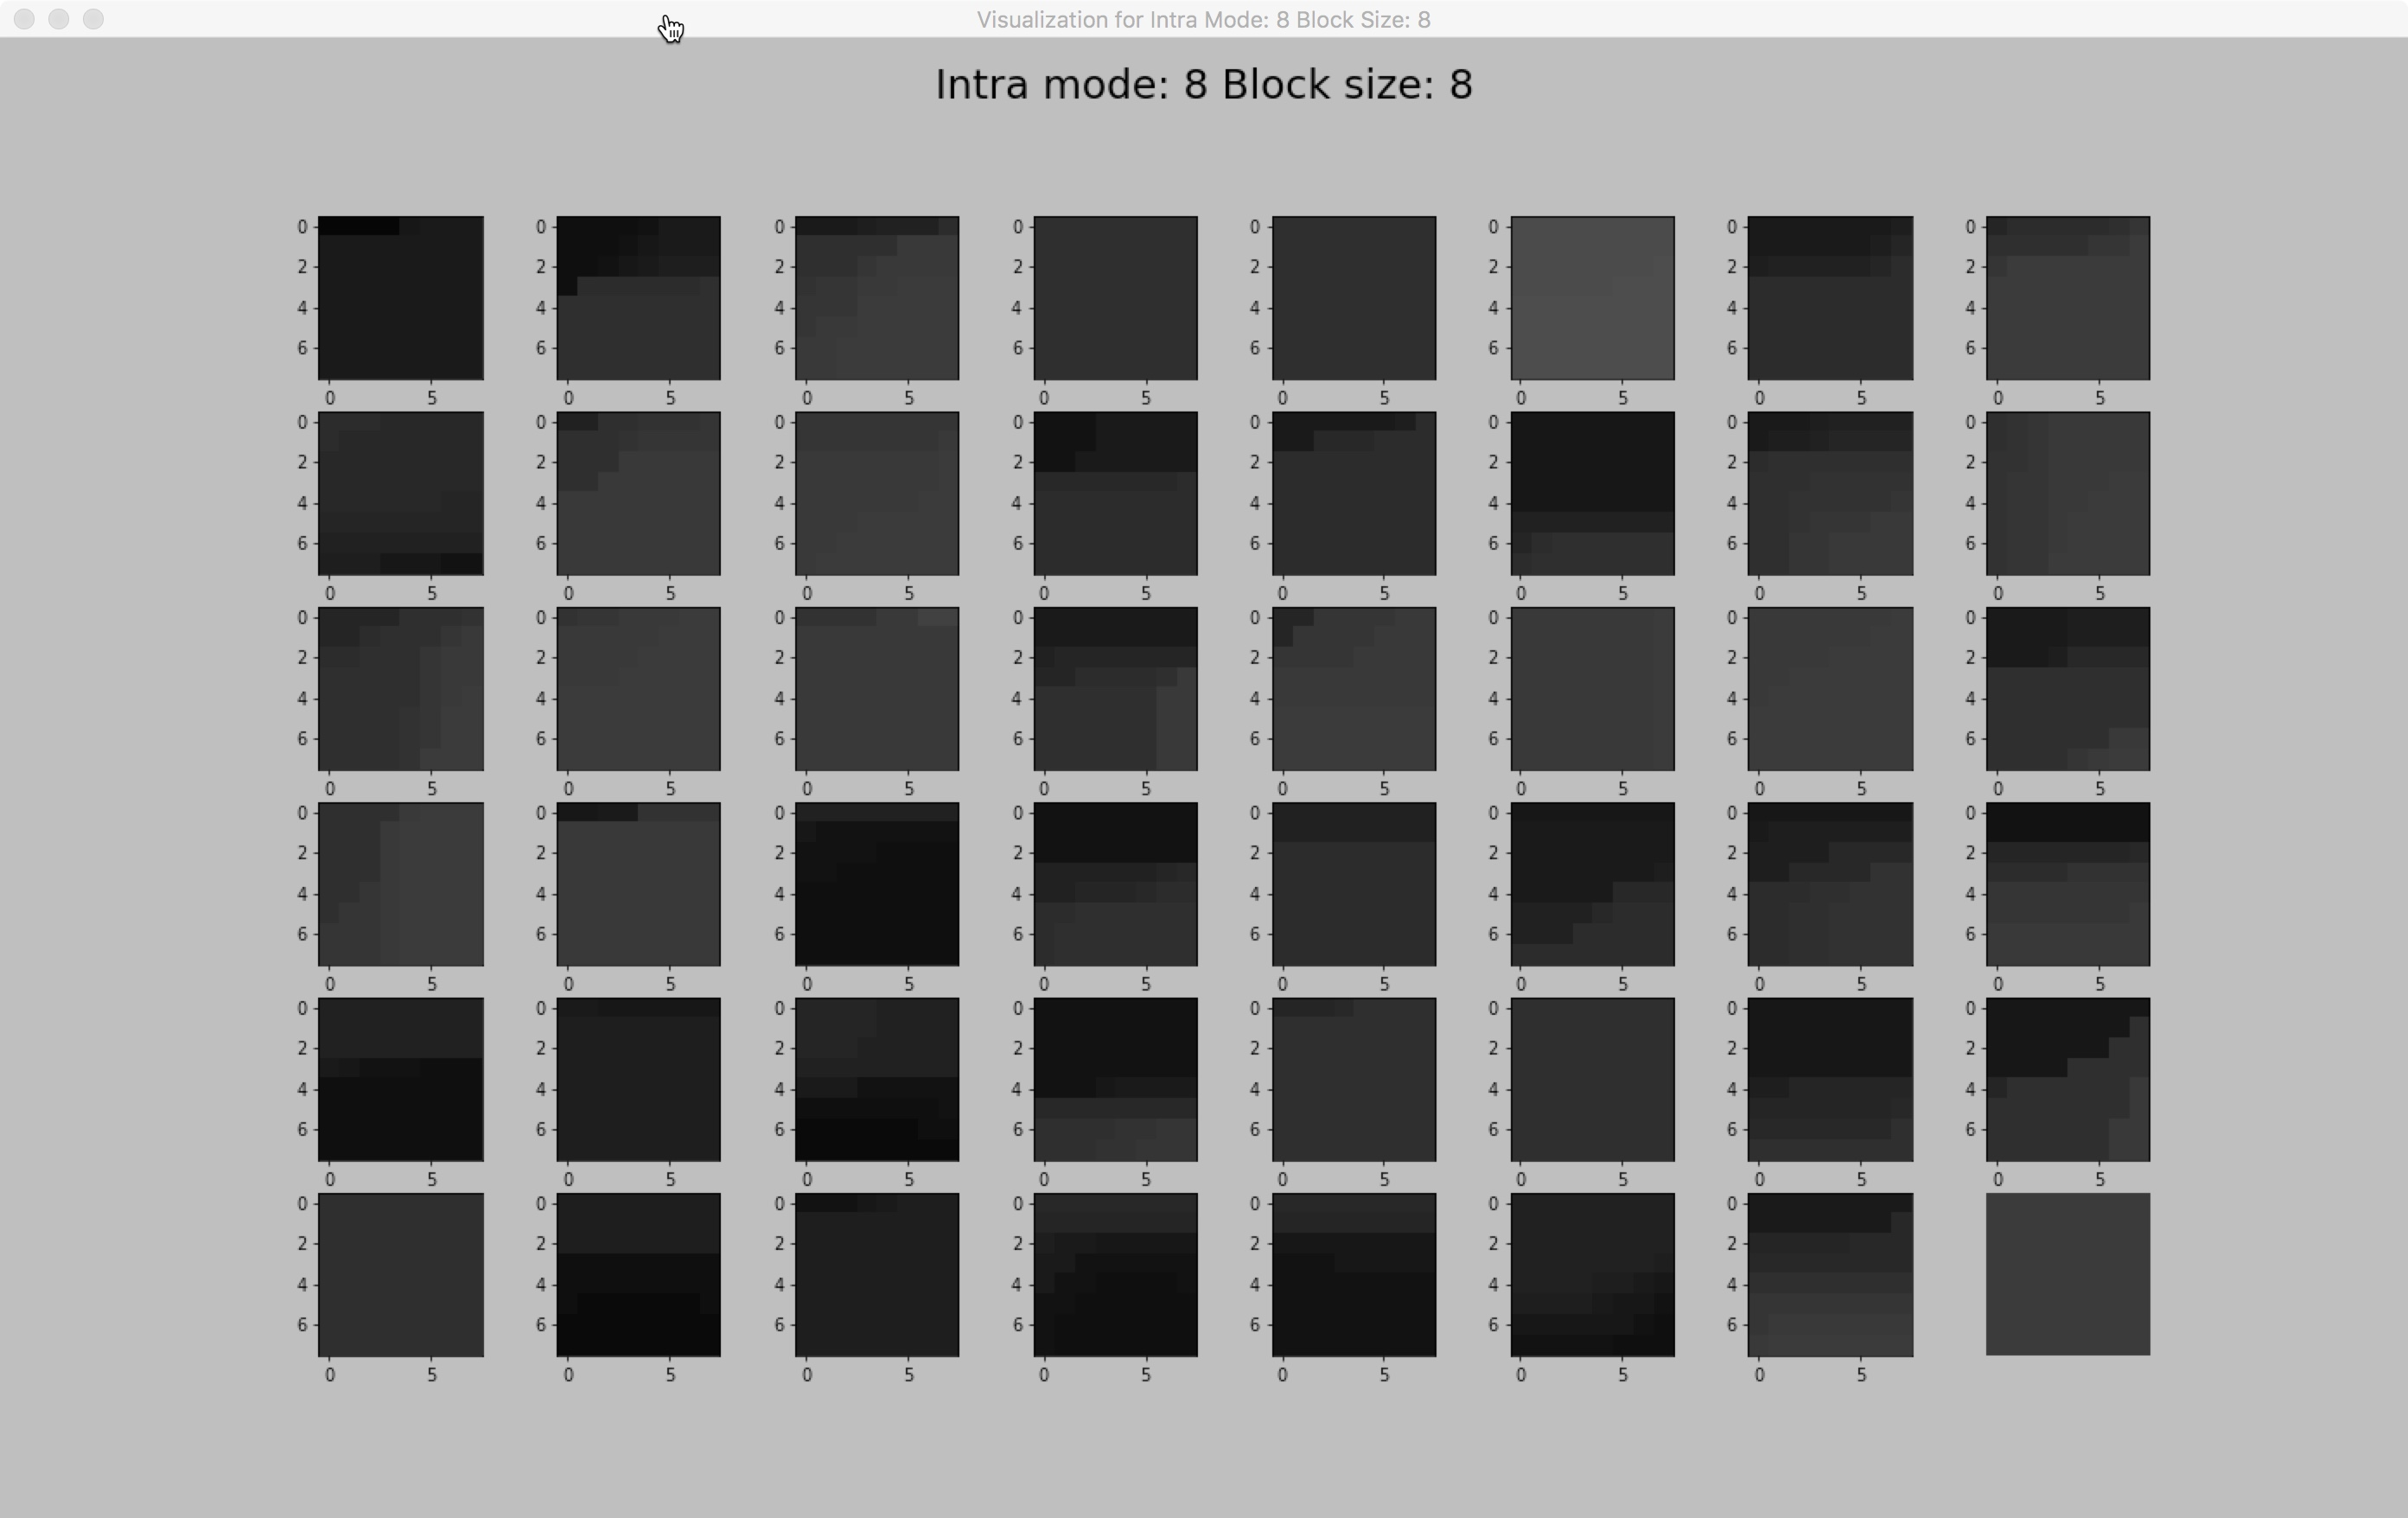
\includegraphics[width=\linewidth]{Figures/visu-size8x8/8-8}
        \caption[Intra mode 8]{intra mode 8.}
        \label{fig:size8_mode8}
    \end{minipage}
    \hspace{\fill} % note: no blank line here
    \begin{minipage}{0.49\textwidth}
        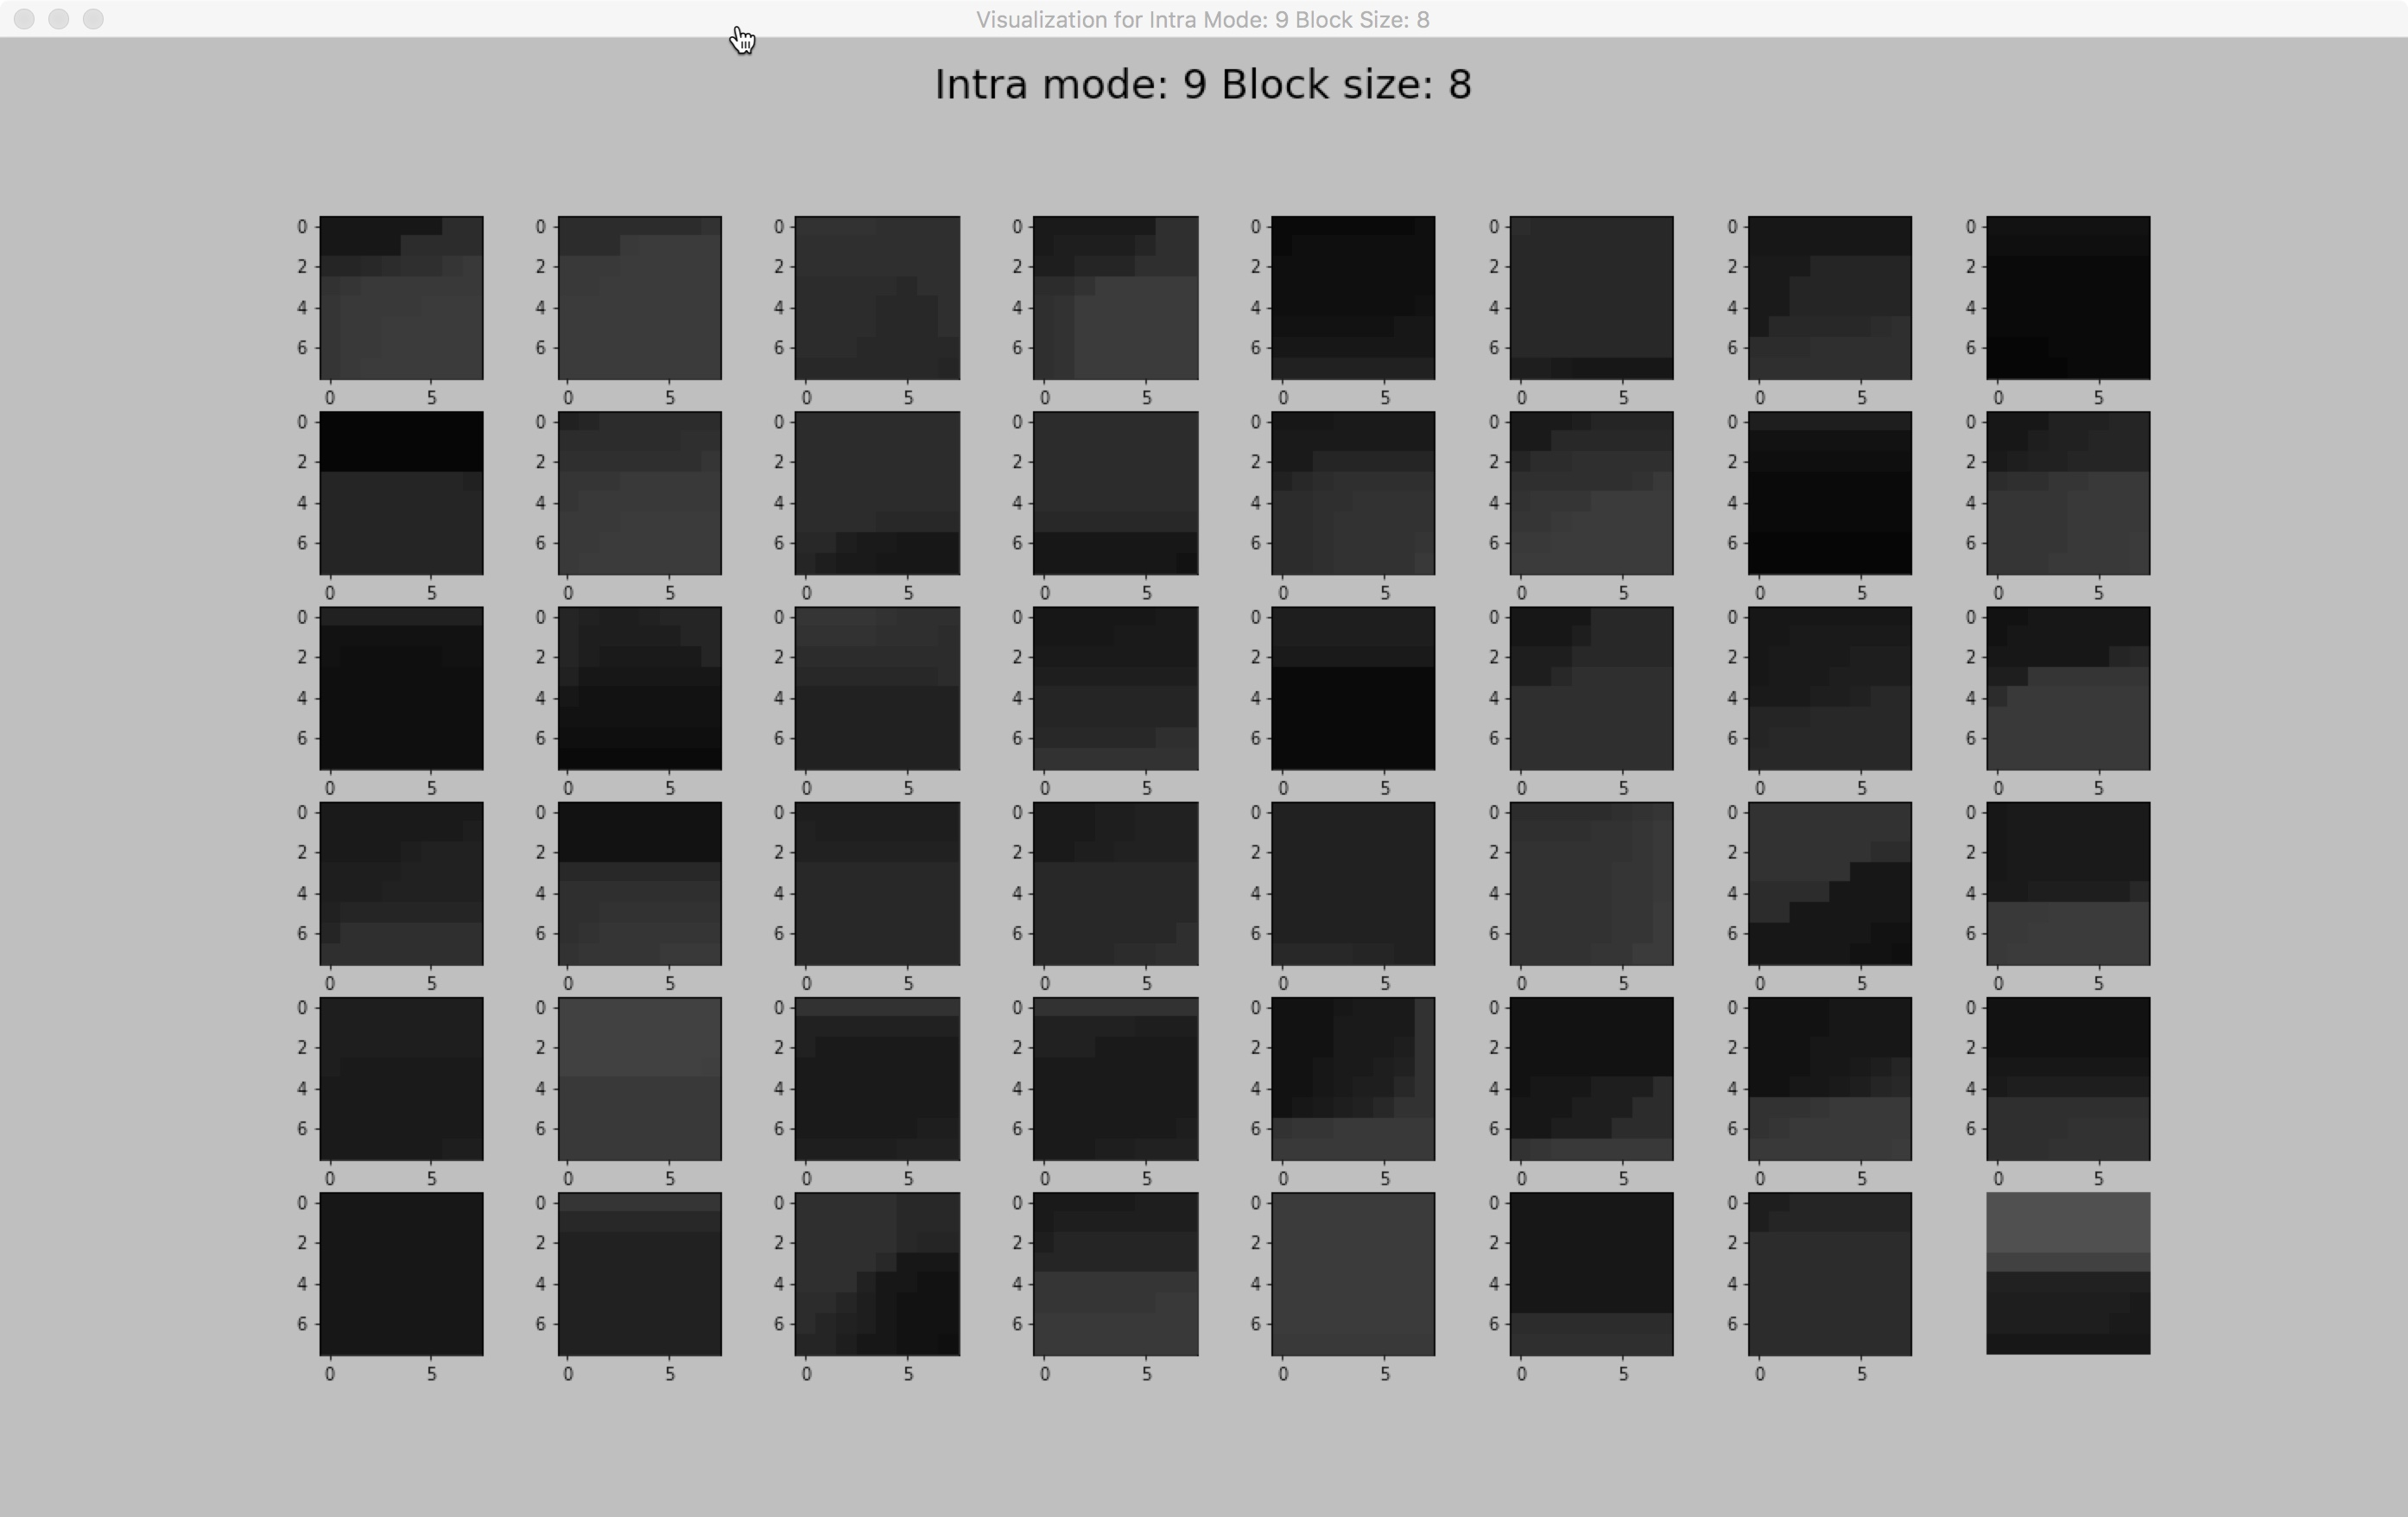
\includegraphics[width=\linewidth]{Figures/visu-size8x8/8-9}
        \caption[Intra mode 9]{intra mode 9.}
        \label{fig:size8_mode9}
    \end{minipage}
% \caption{Figure caption goes here}\label{fig:visualizations-for-blocks-of-size8x8-01}
\end{figure}

\begin{figure}[H]

    \vspace*{1cm} % vertical separation

    \begin{minipage}{0.49\textwidth}
        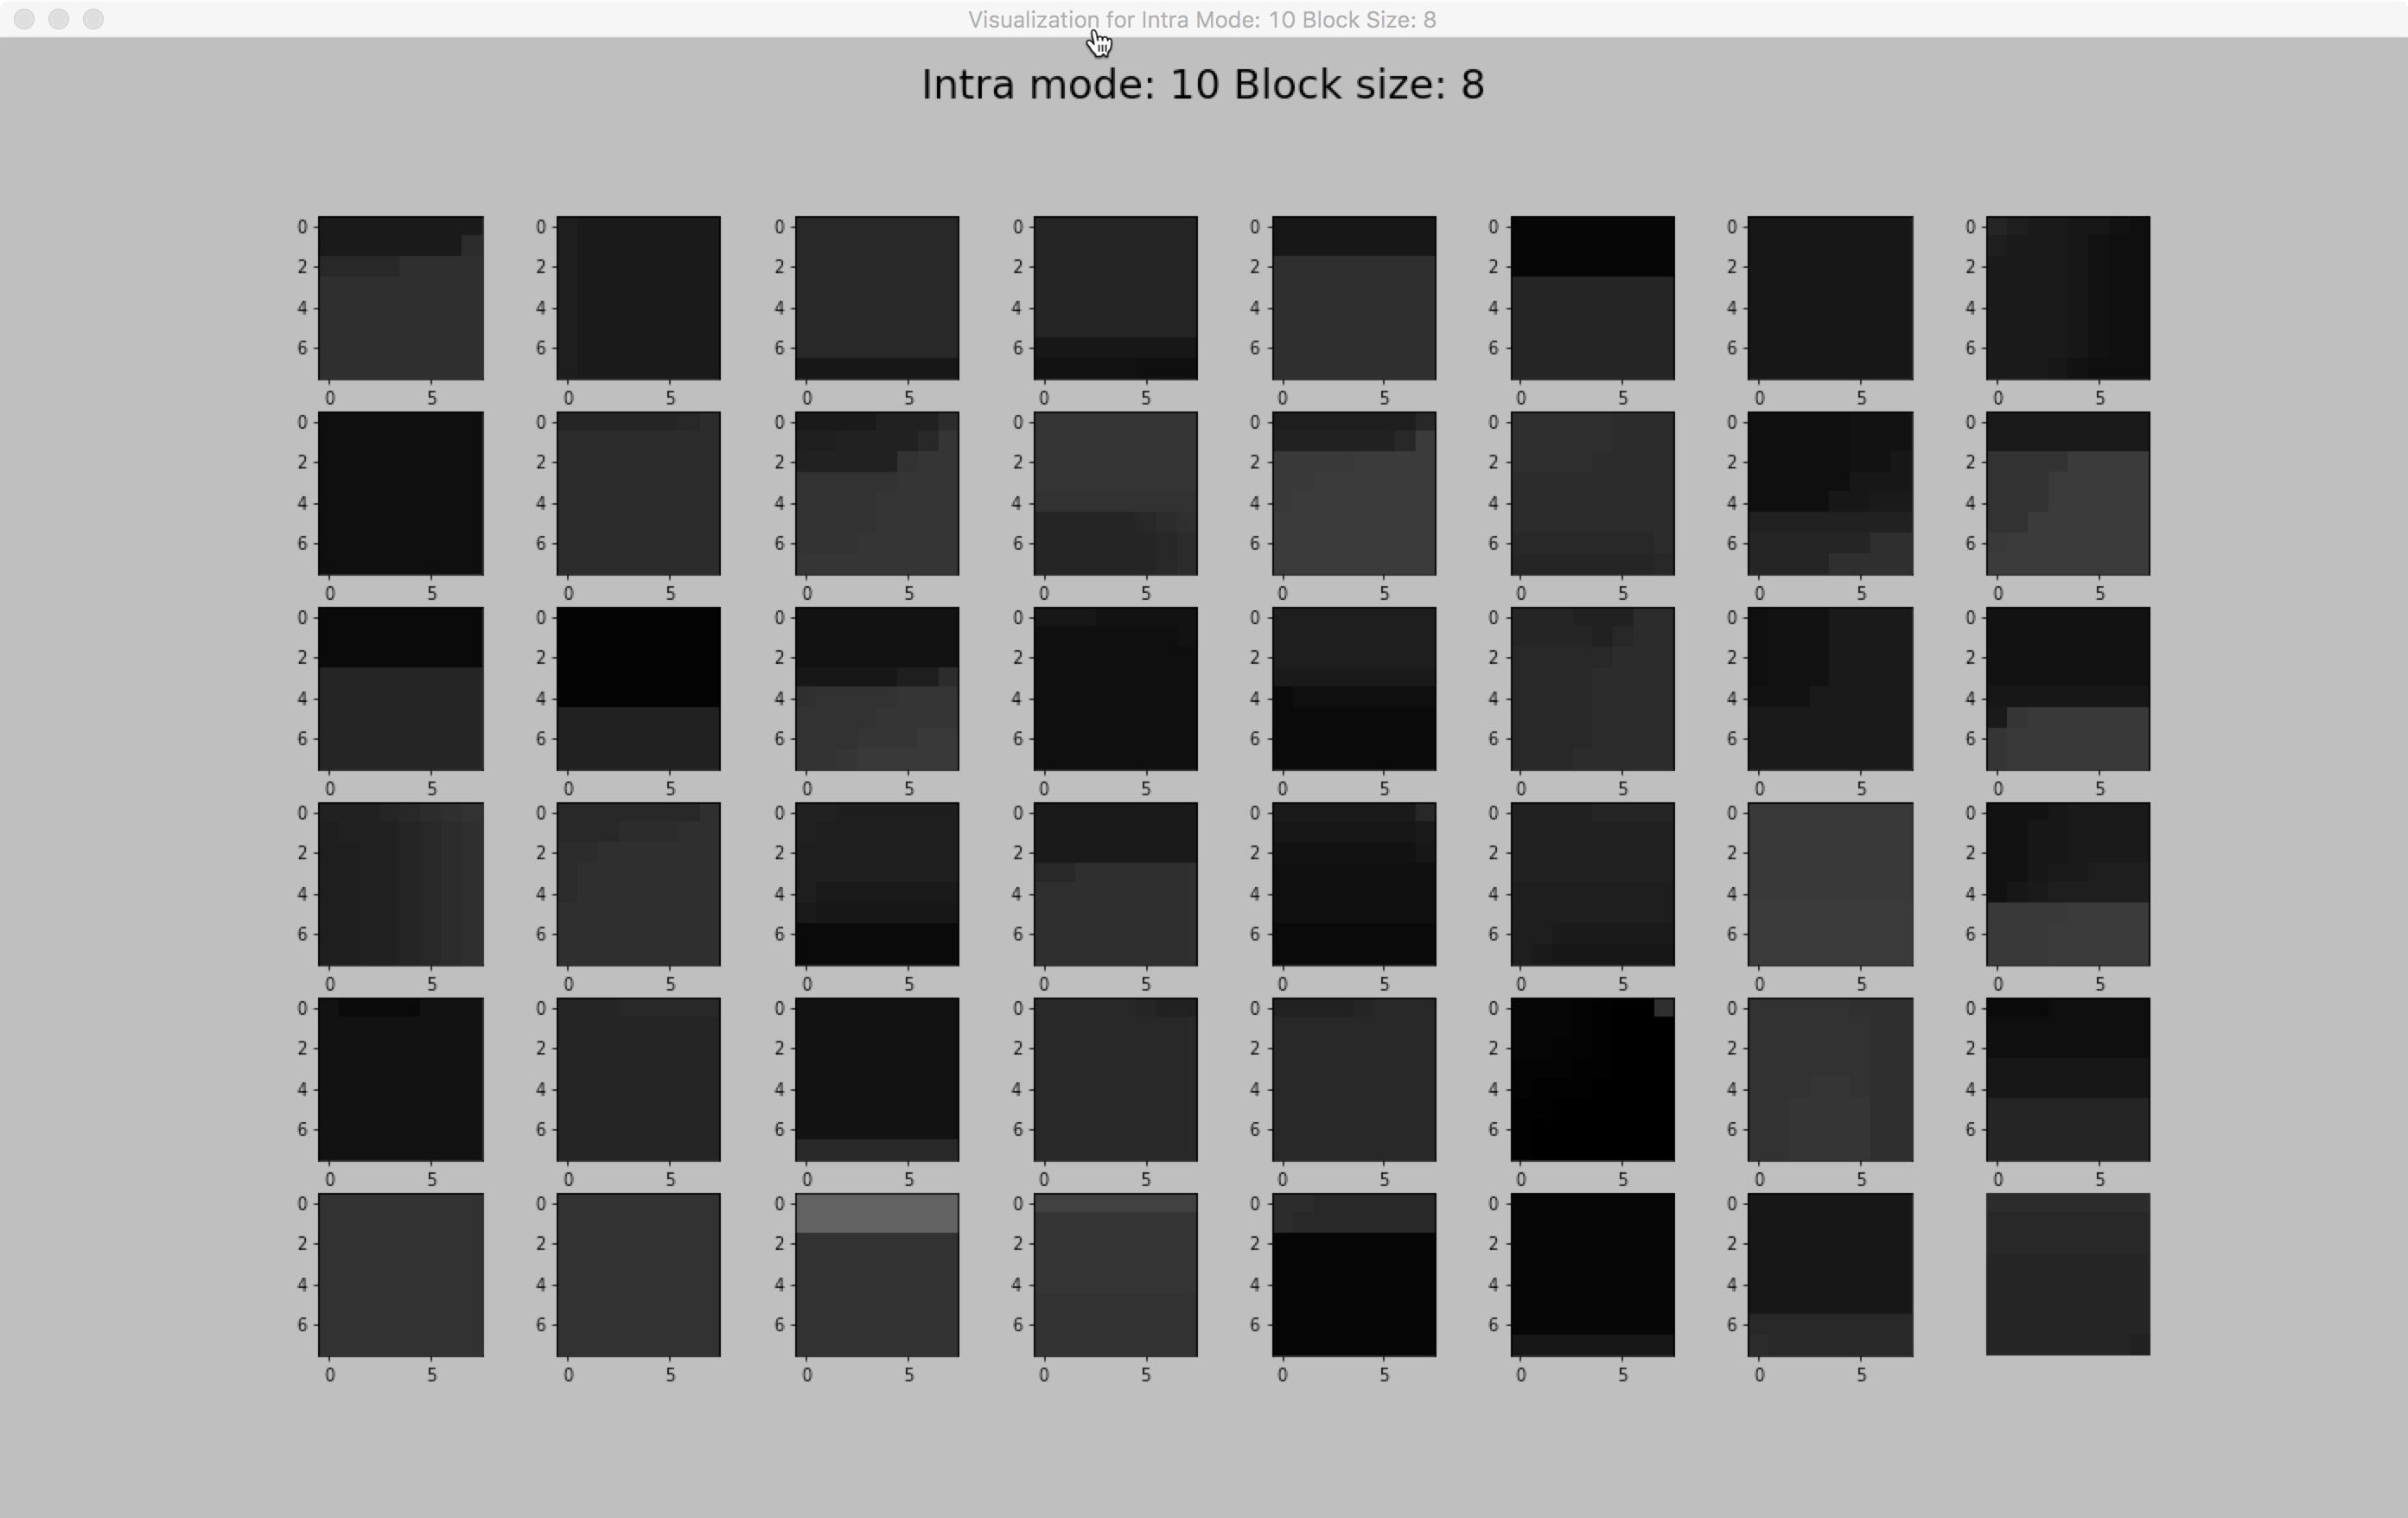
\includegraphics[width=\linewidth]{Figures/visu-size8x8/8-10}
        \caption[Intra mode 10]{intra mode 10.}
        \label{fig:size8_mode4}
    \end{minipage}
    \hspace{\fill} % note: no blank line here
    \begin{minipage}{0.49\textwidth}
        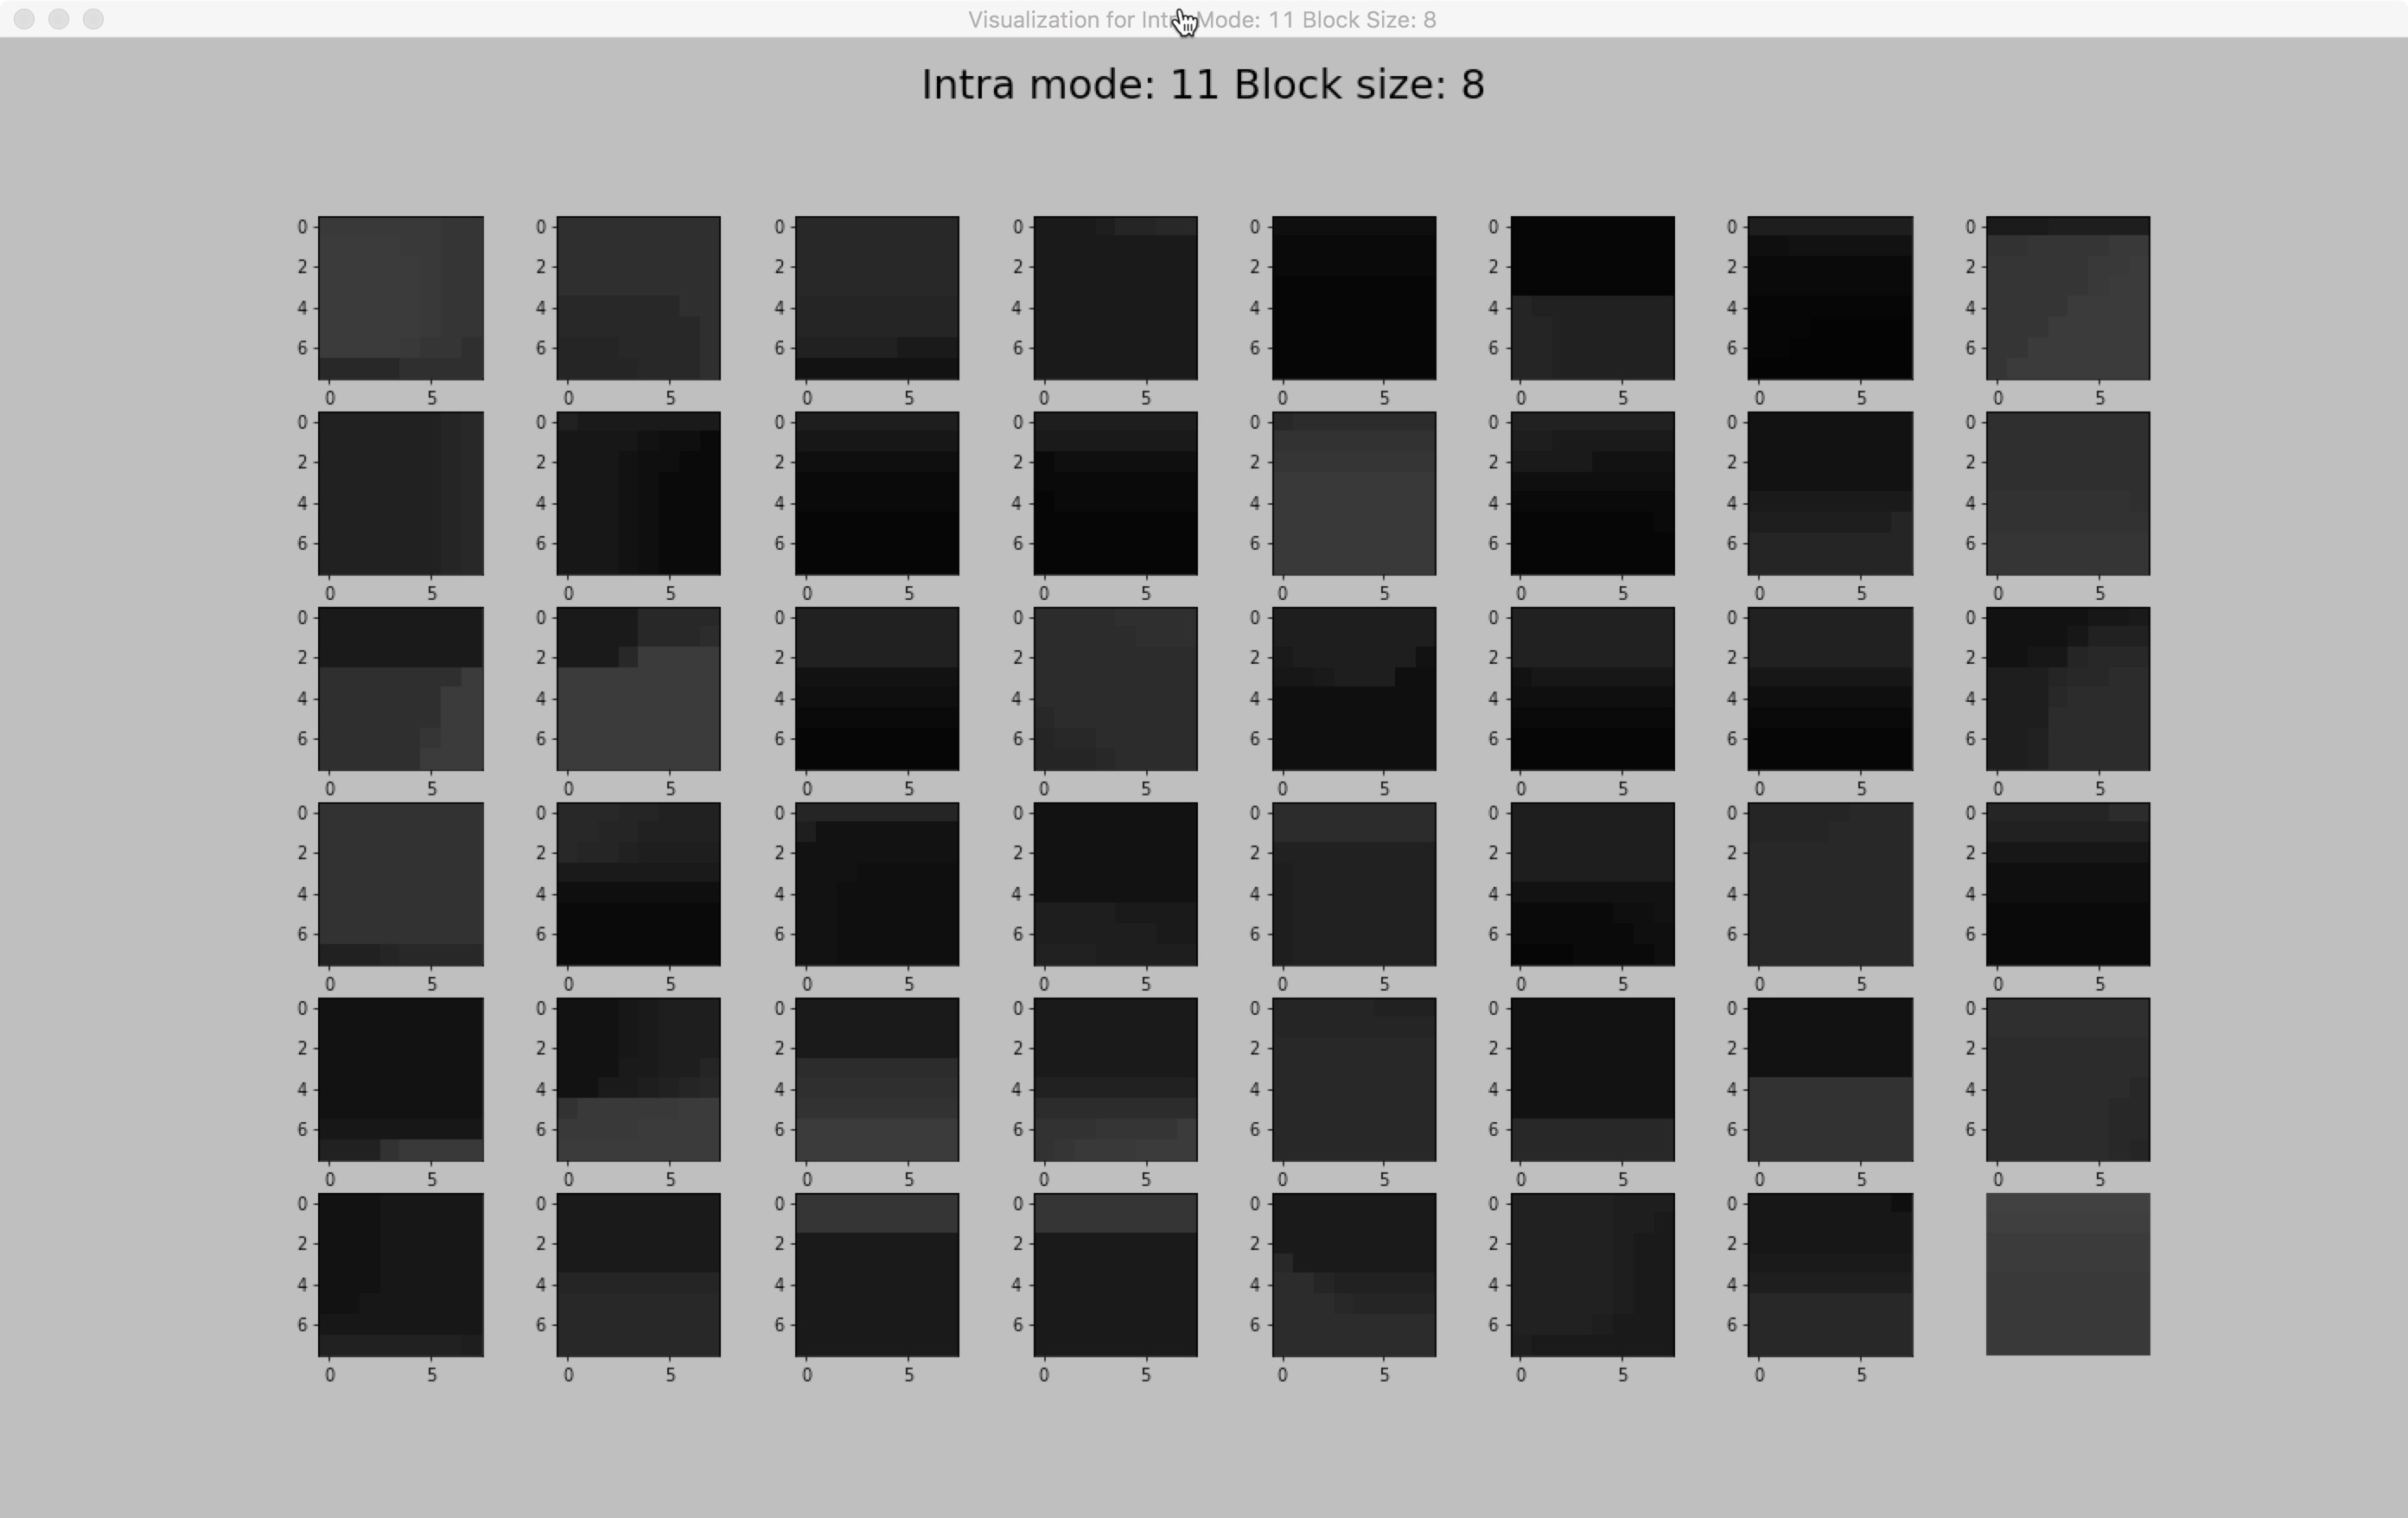
\includegraphics[width=\linewidth]{Figures/visu-size8x8/8-11}
        \caption[Intra mode 11]{intra mode 11.}
        \label{fig:size8_mode11}
    \end{minipage}
    
    \vspace*{1cm} % vertical separation
    
    \begin{minipage}{0.49\textwidth}
        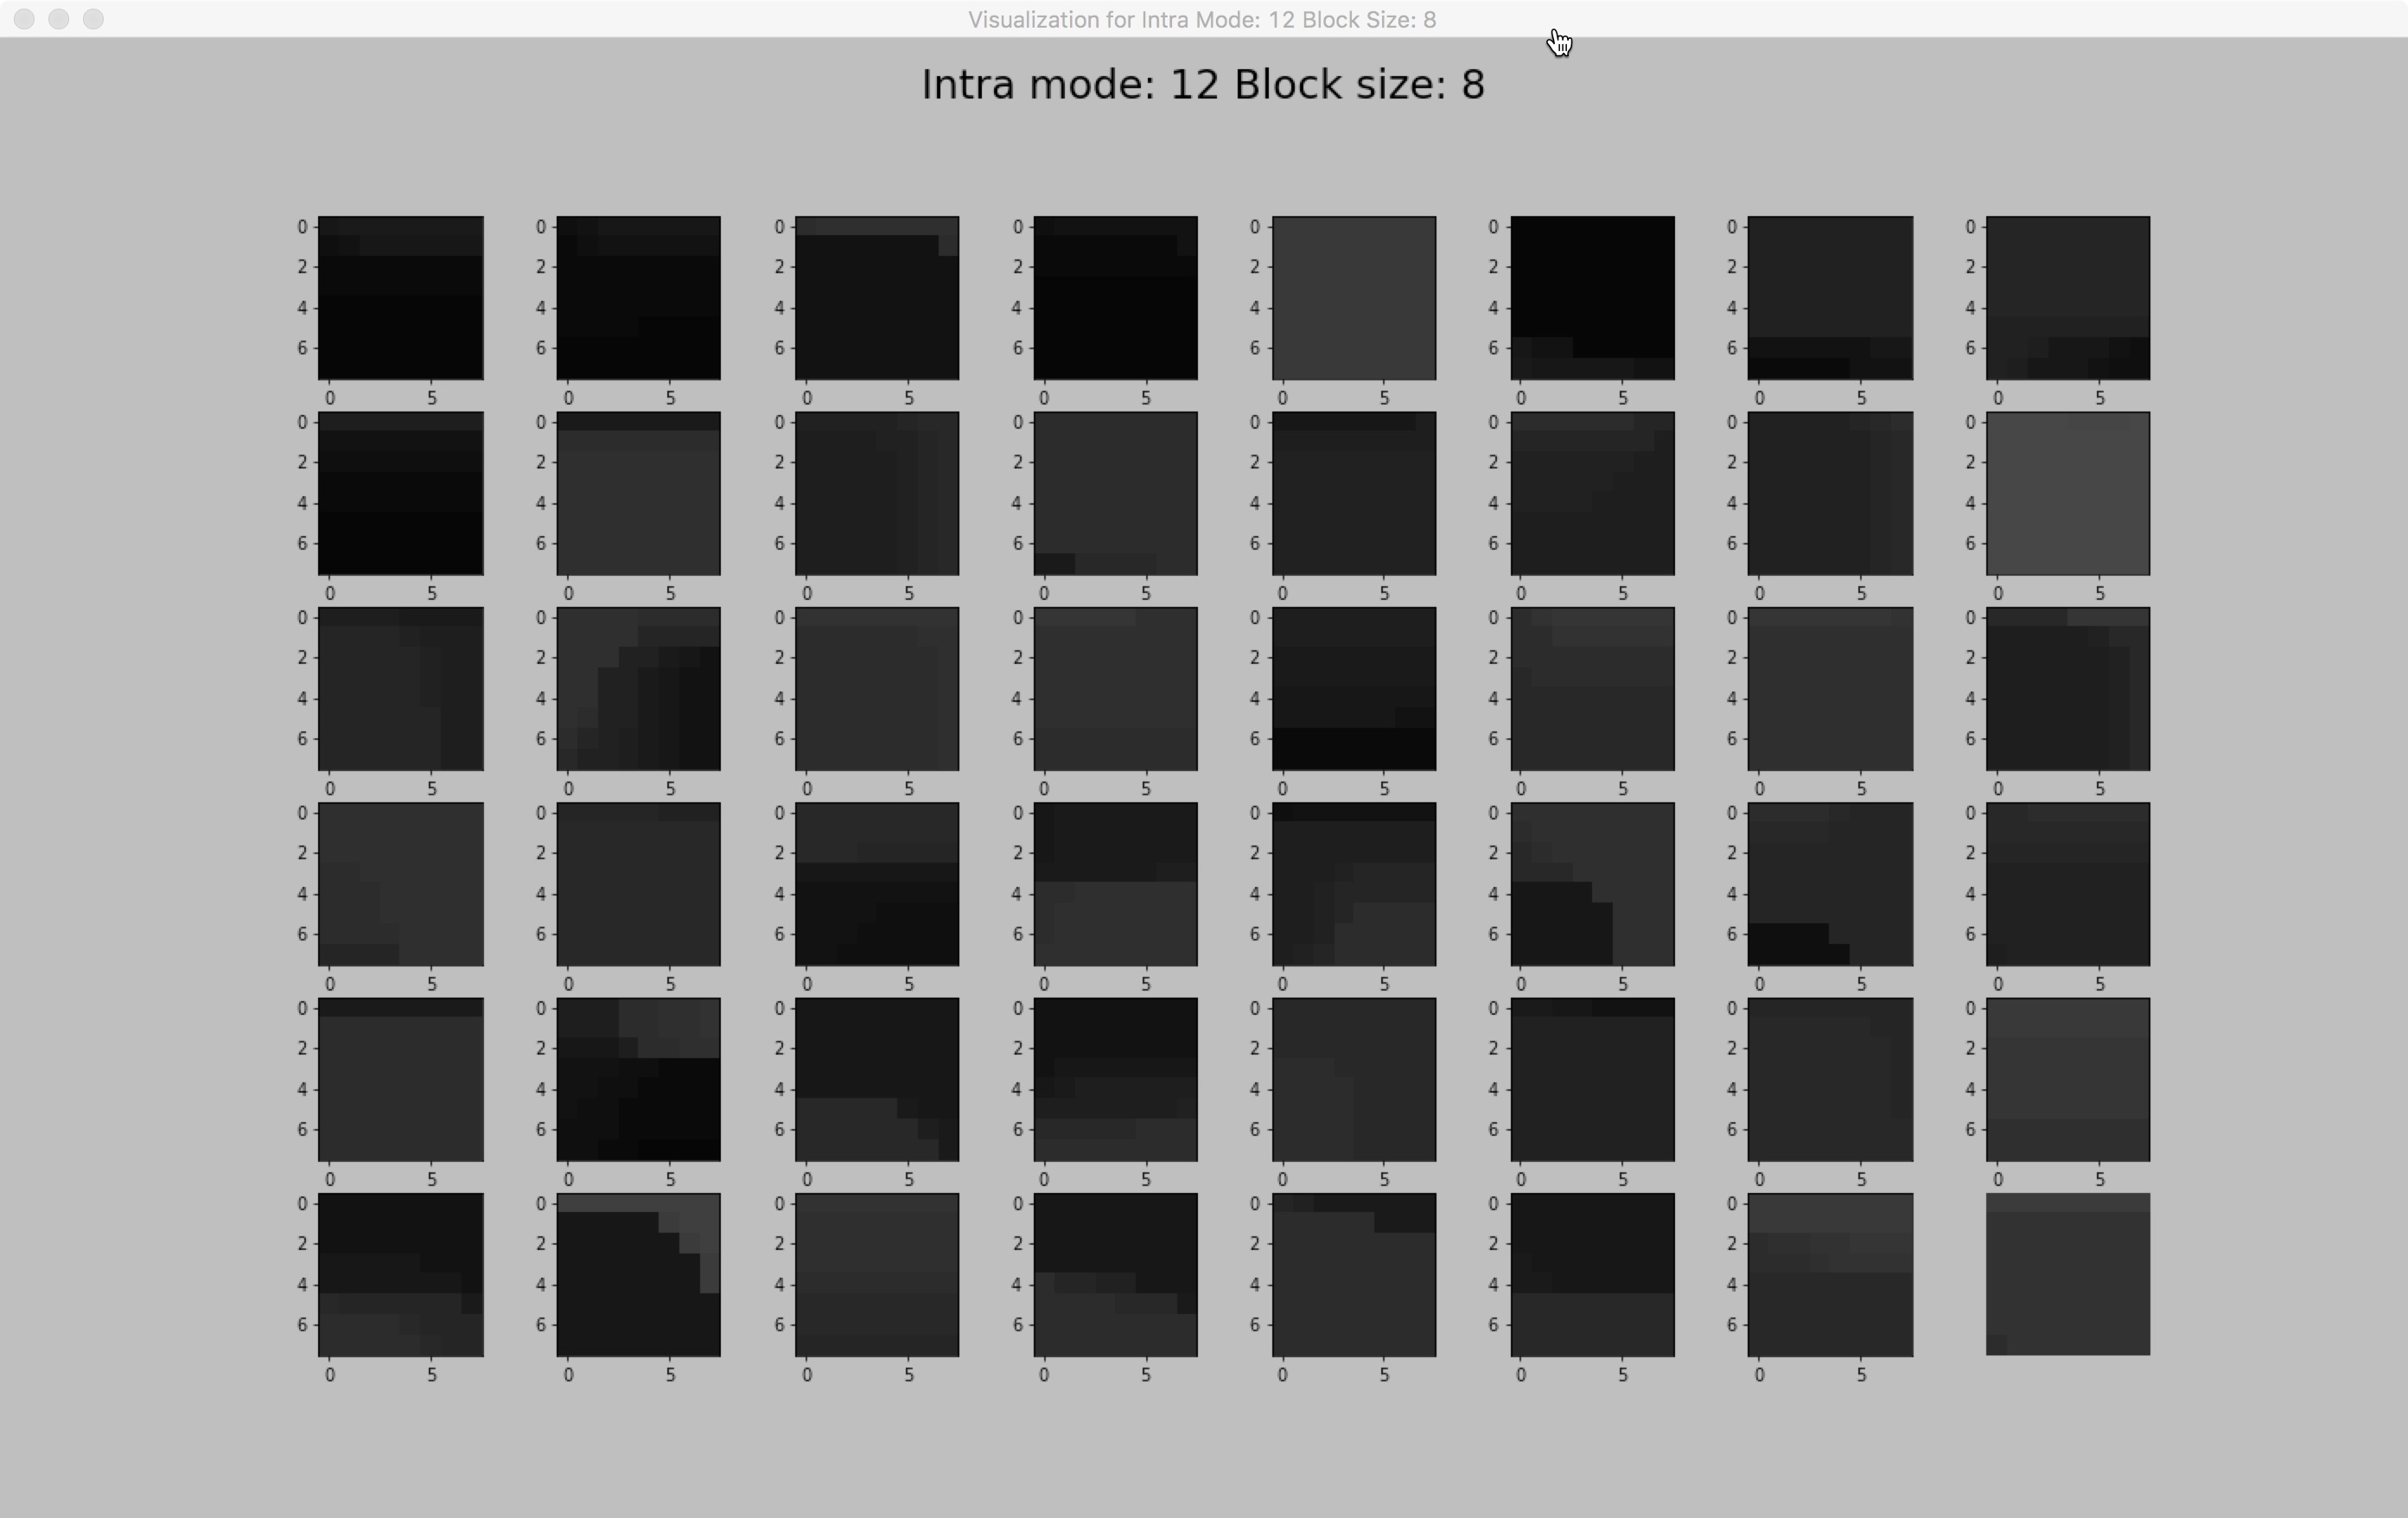
\includegraphics[width=\linewidth]{Figures/visu-size8x8/8-12}
        \caption[Intra mode 12]{intra mode 12.}
        \label{fig:size8_mode12}
    \end{minipage}
    \hspace{\fill} % note: no blank line here
    \begin{minipage}{0.49\textwidth}
        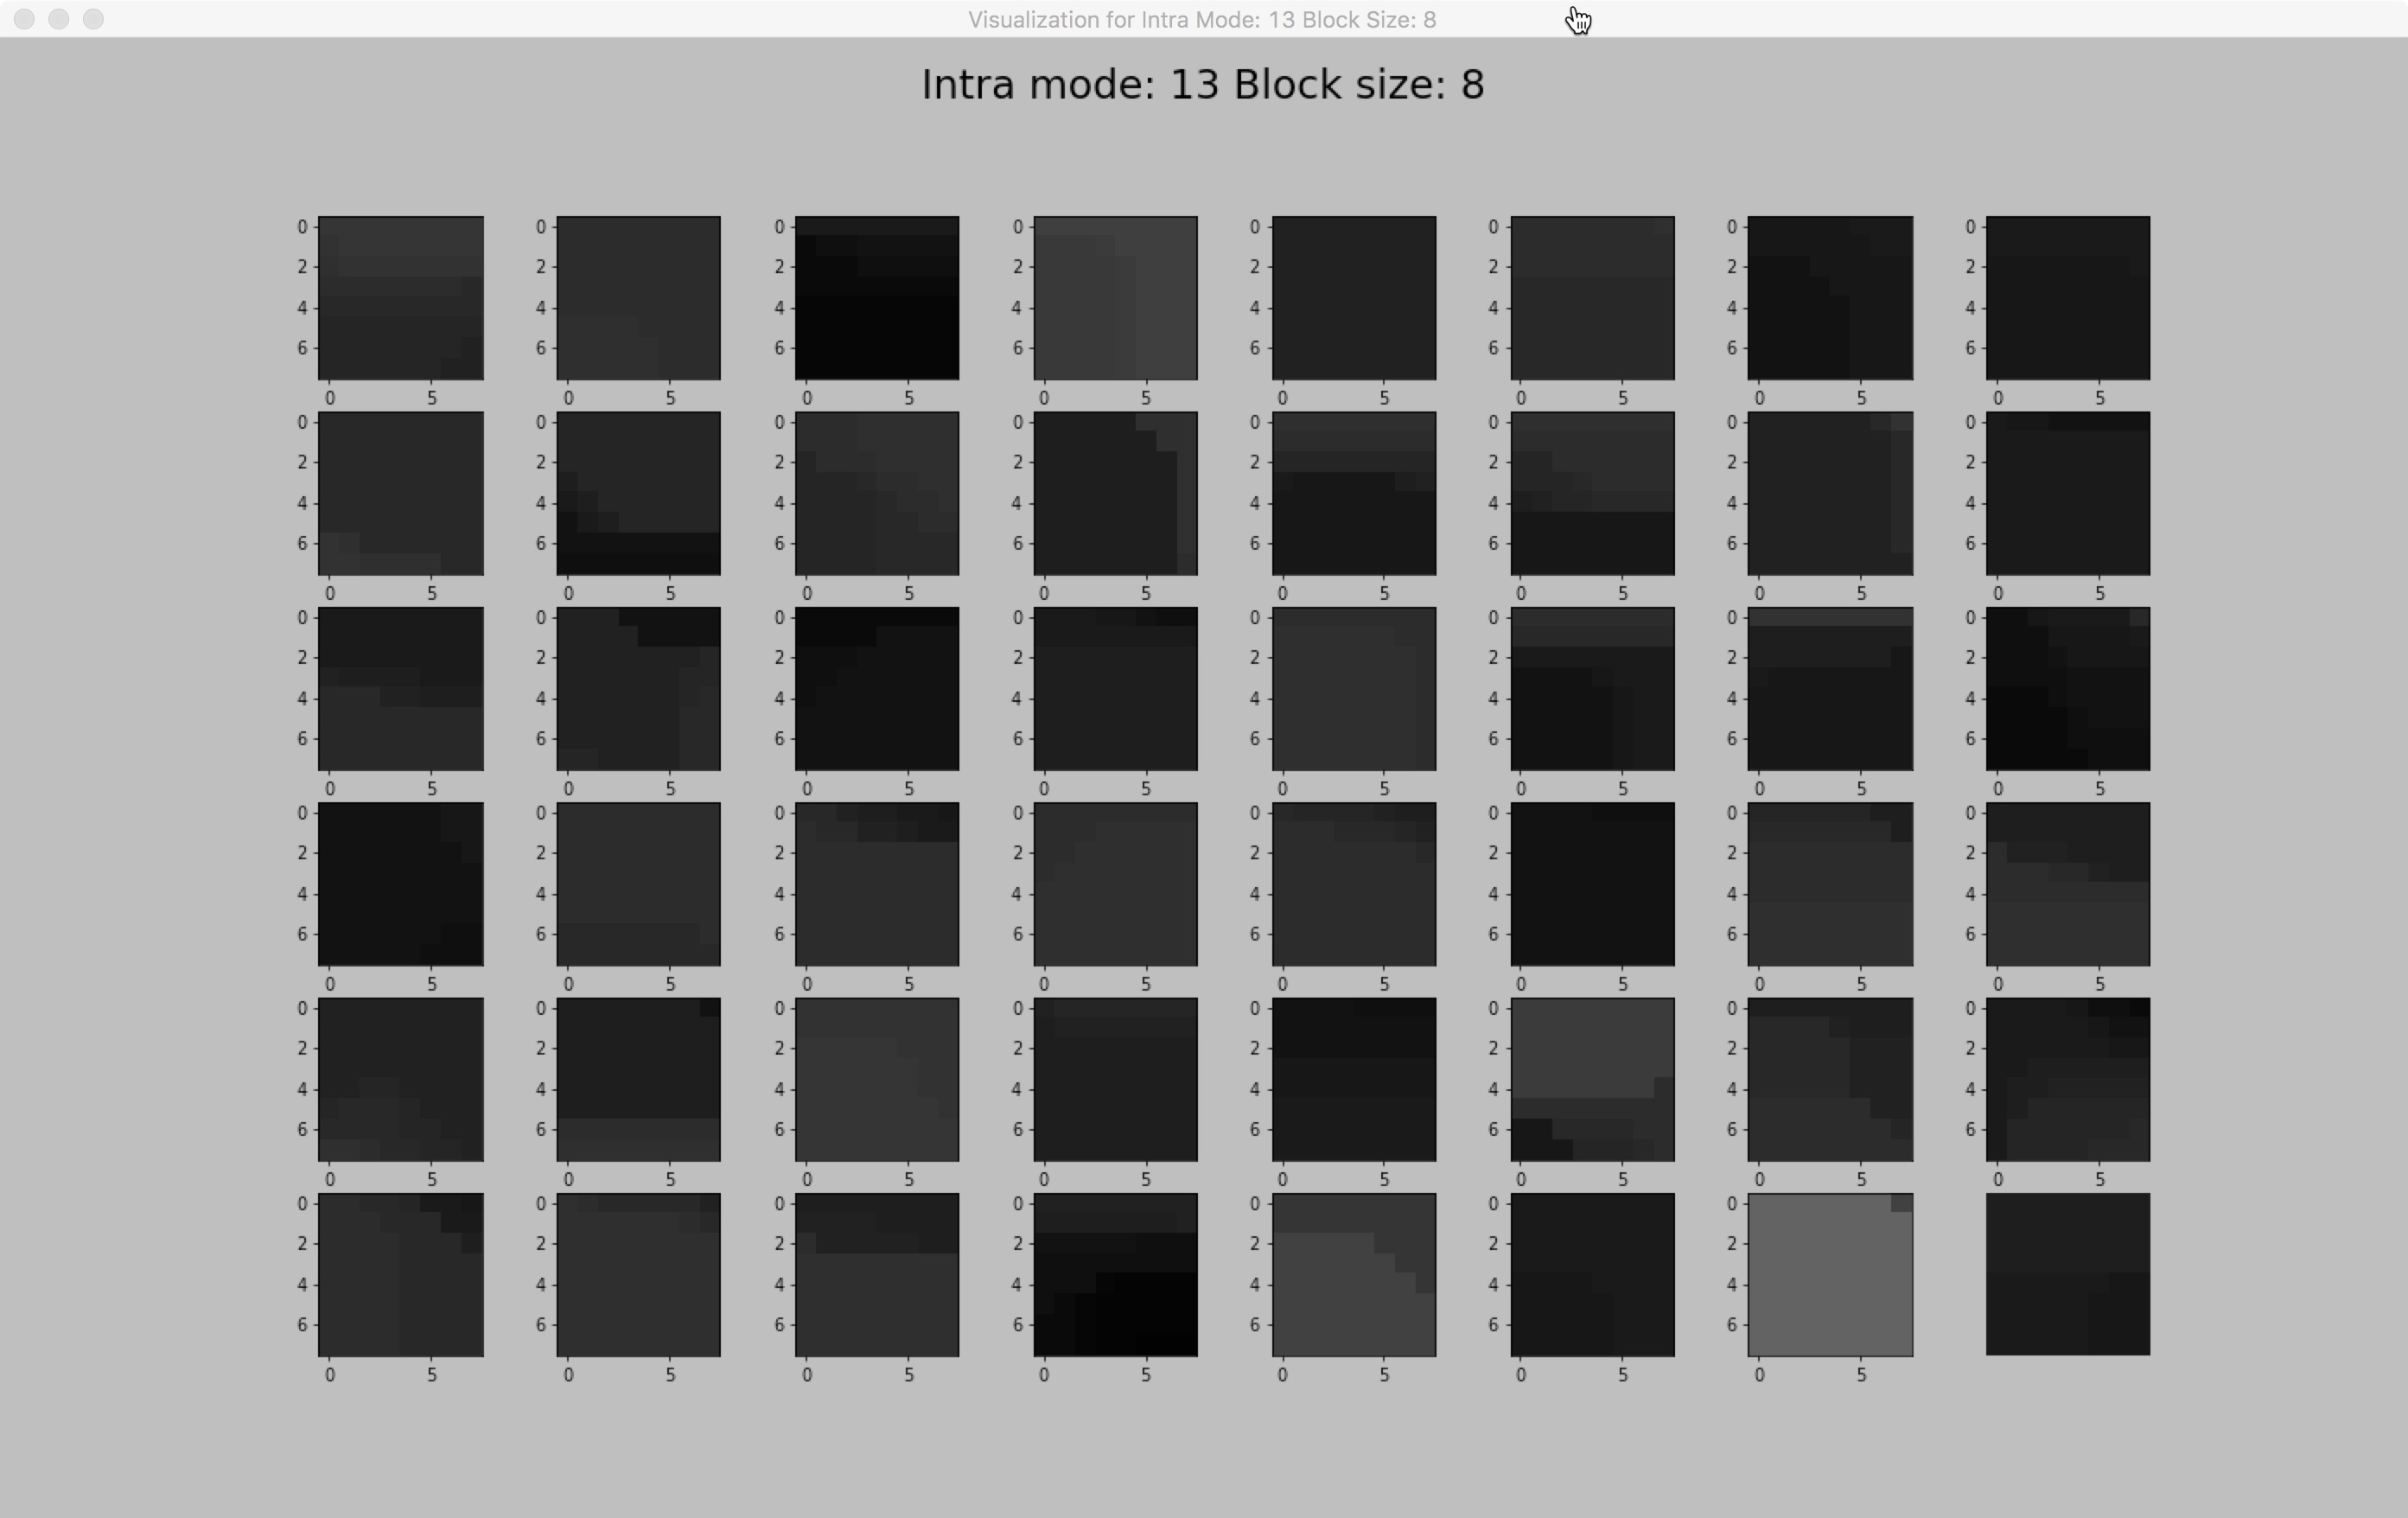
\includegraphics[width=\linewidth]{Figures/visu-size8x8/8-13}
        \caption[Intra mode 13]{intra mode 13.}
        \label{fig:size8_mode13}
    \end{minipage}
    
    \vspace*{1cm} % vertical separation

    \begin{minipage}{0.49\textwidth}
        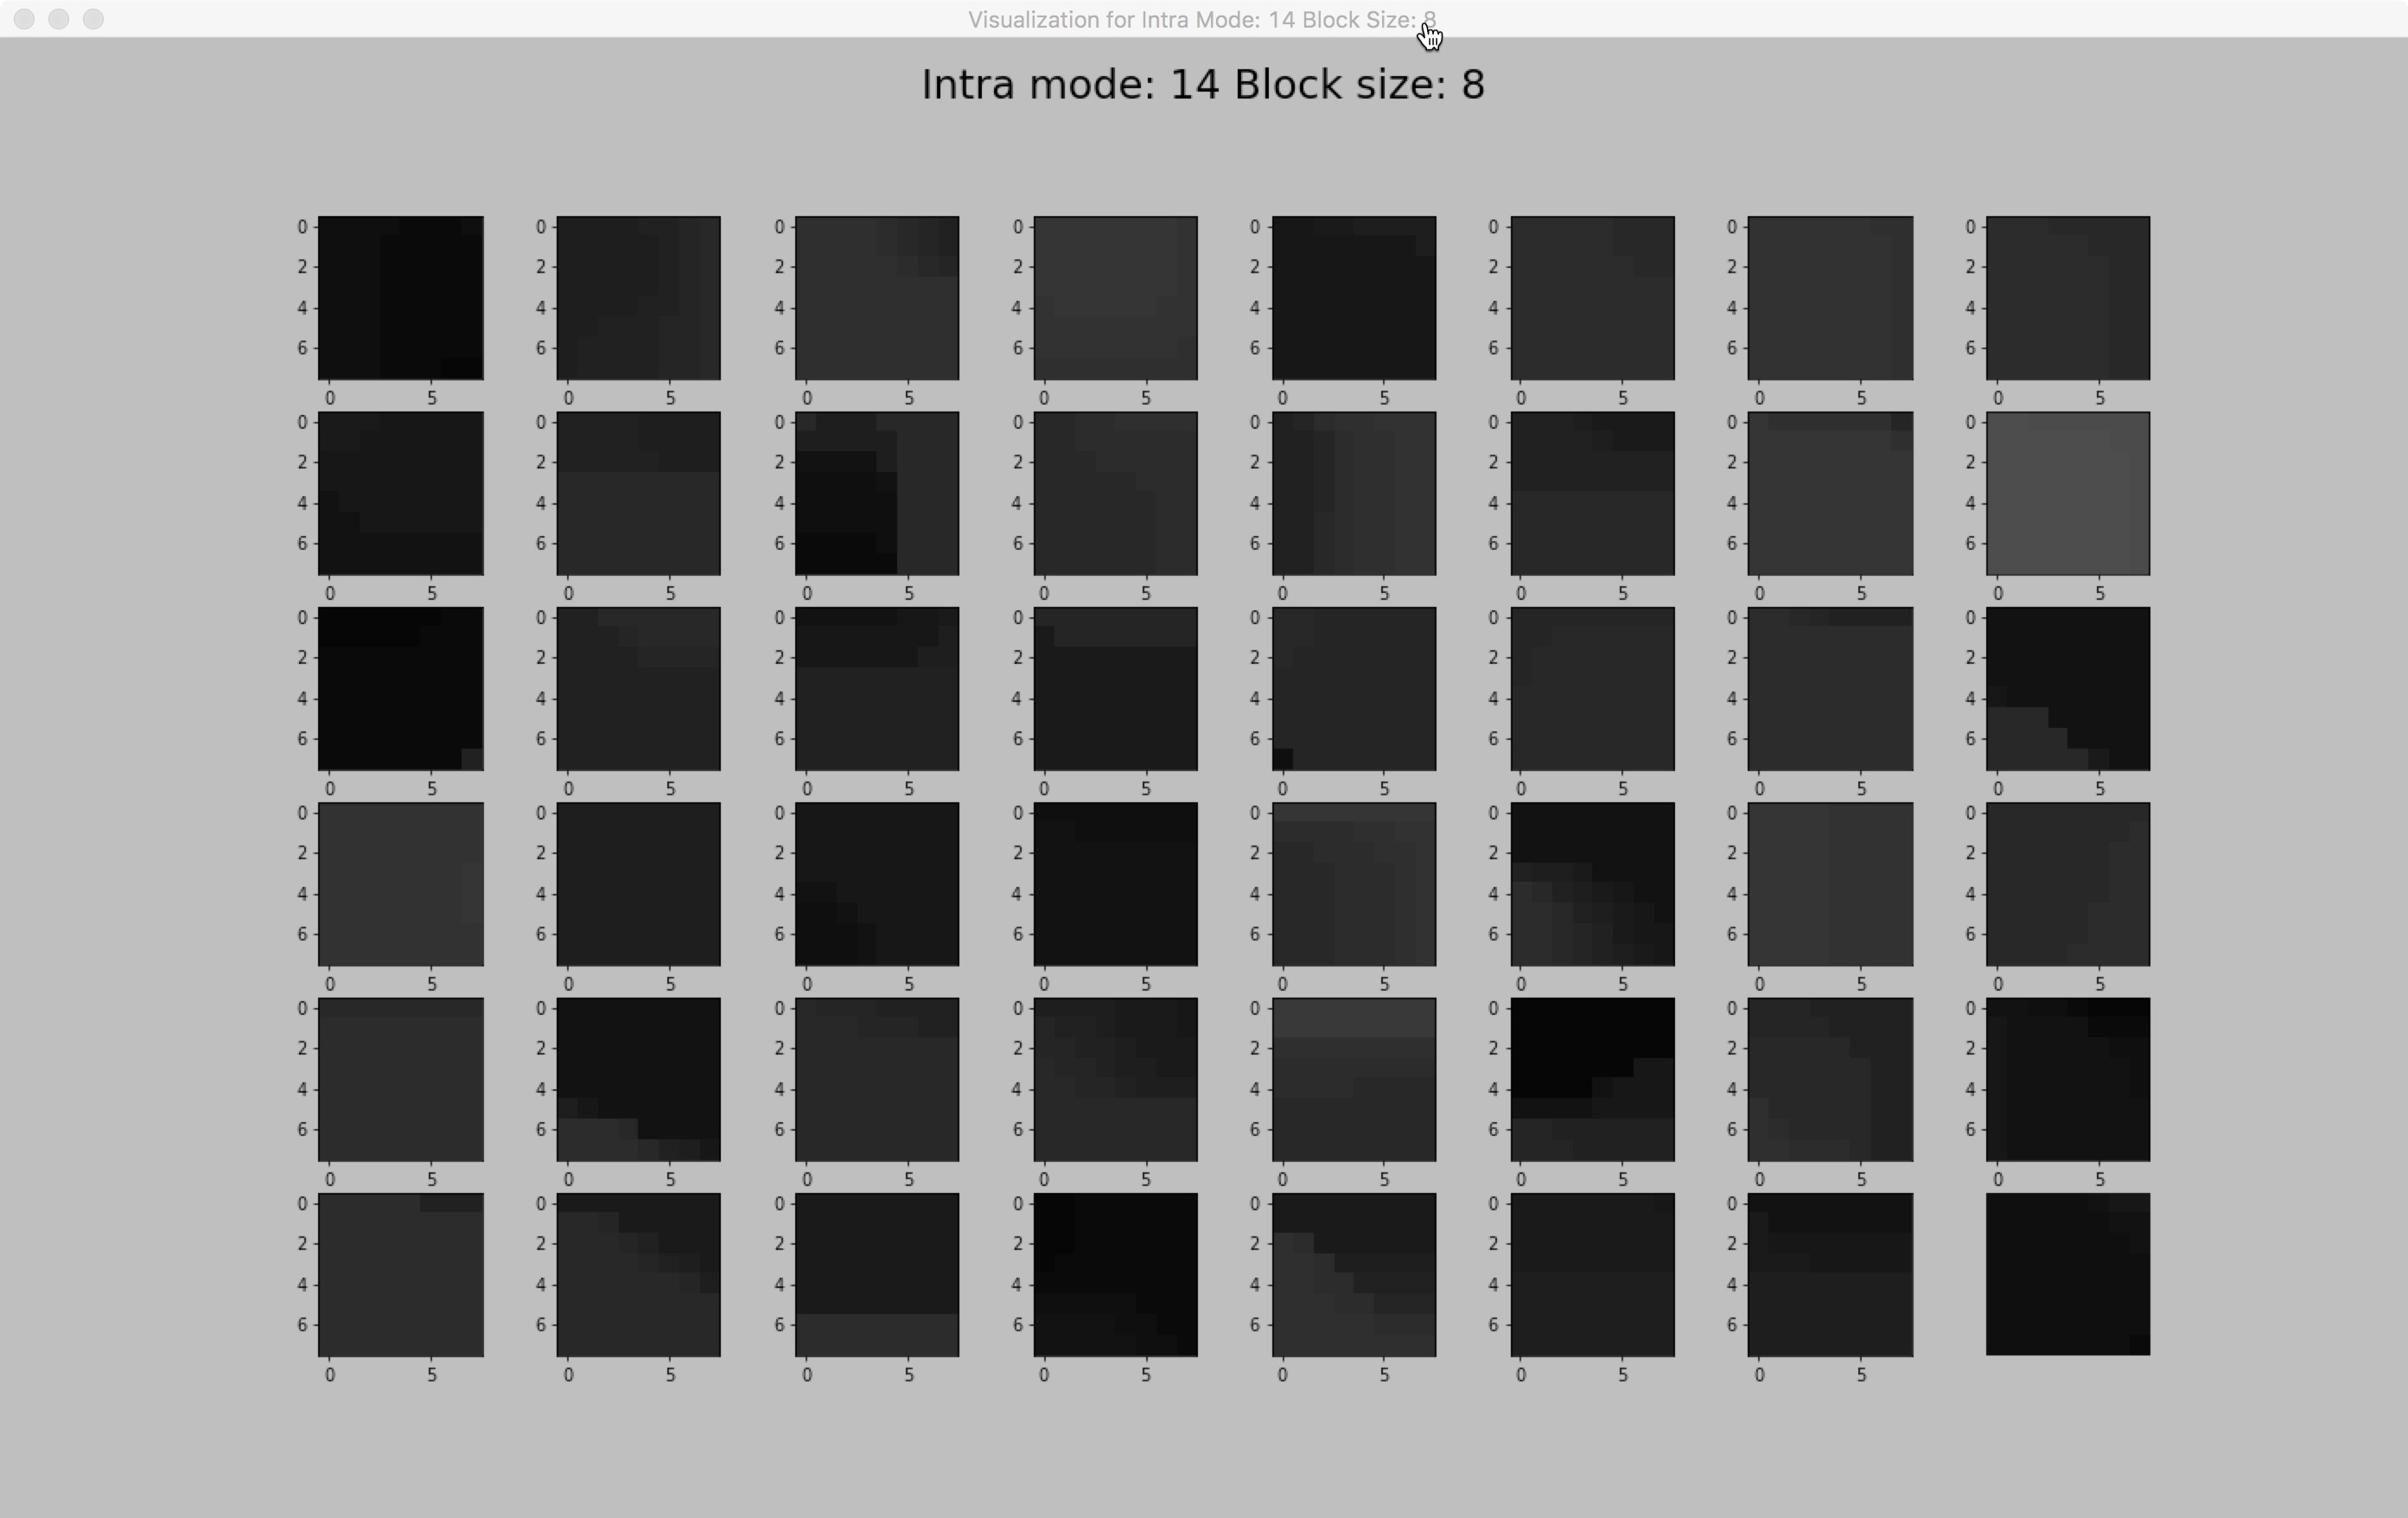
\includegraphics[width=\linewidth]{Figures/visu-size8x8/8-14}
        \caption[Intra mode 14]{intra mode 14.}
        \label{fig:size8_mode14}
    \end{minipage}
    \hspace{\fill} % note: no blank line here
    \begin{minipage}{0.49\textwidth}
        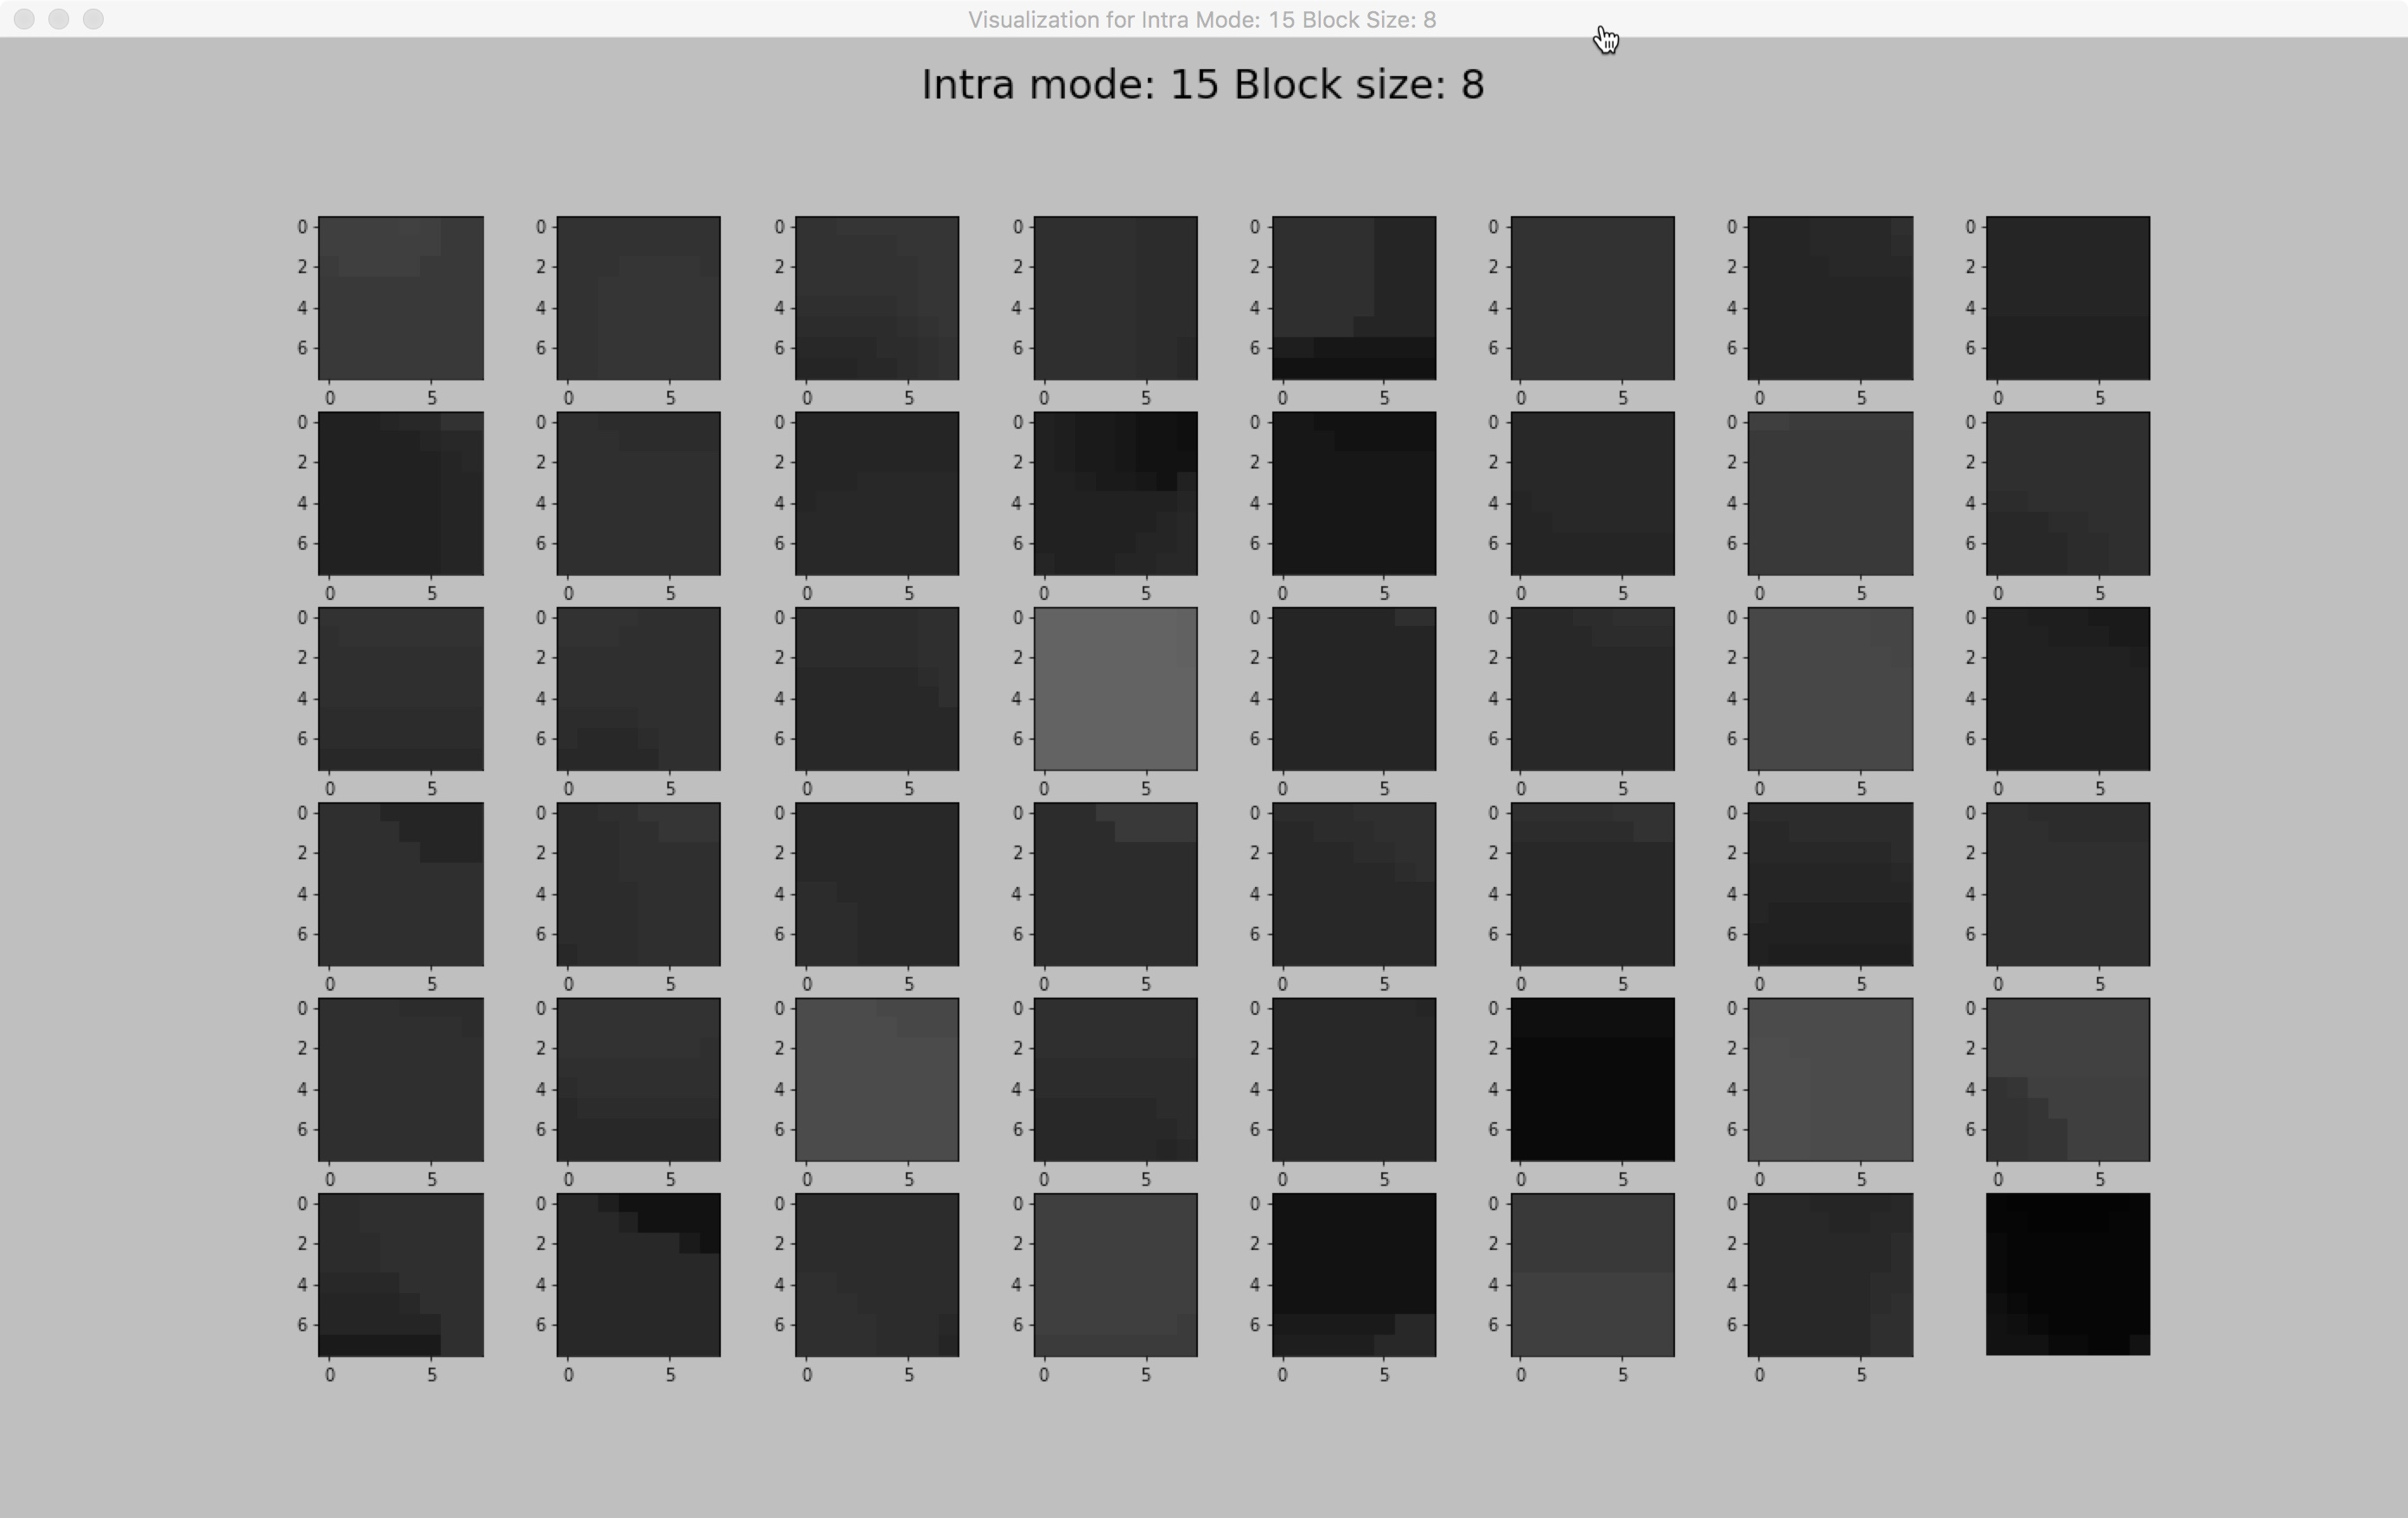
\includegraphics[width=\linewidth]{Figures/visu-size8x8/8-15}
        \caption[Intra mode 15]{intra mode 15.}
        \label{fig:size8_mode15}
    \end{minipage}
% \caption{Figure caption goes here}\label{fig:visualizations-for-blocks-of-size8x8-01}
\end{figure}

\begin{figure}[H]

    \vspace*{1cm} % vertical separation

    \begin{minipage}{0.49\textwidth}
        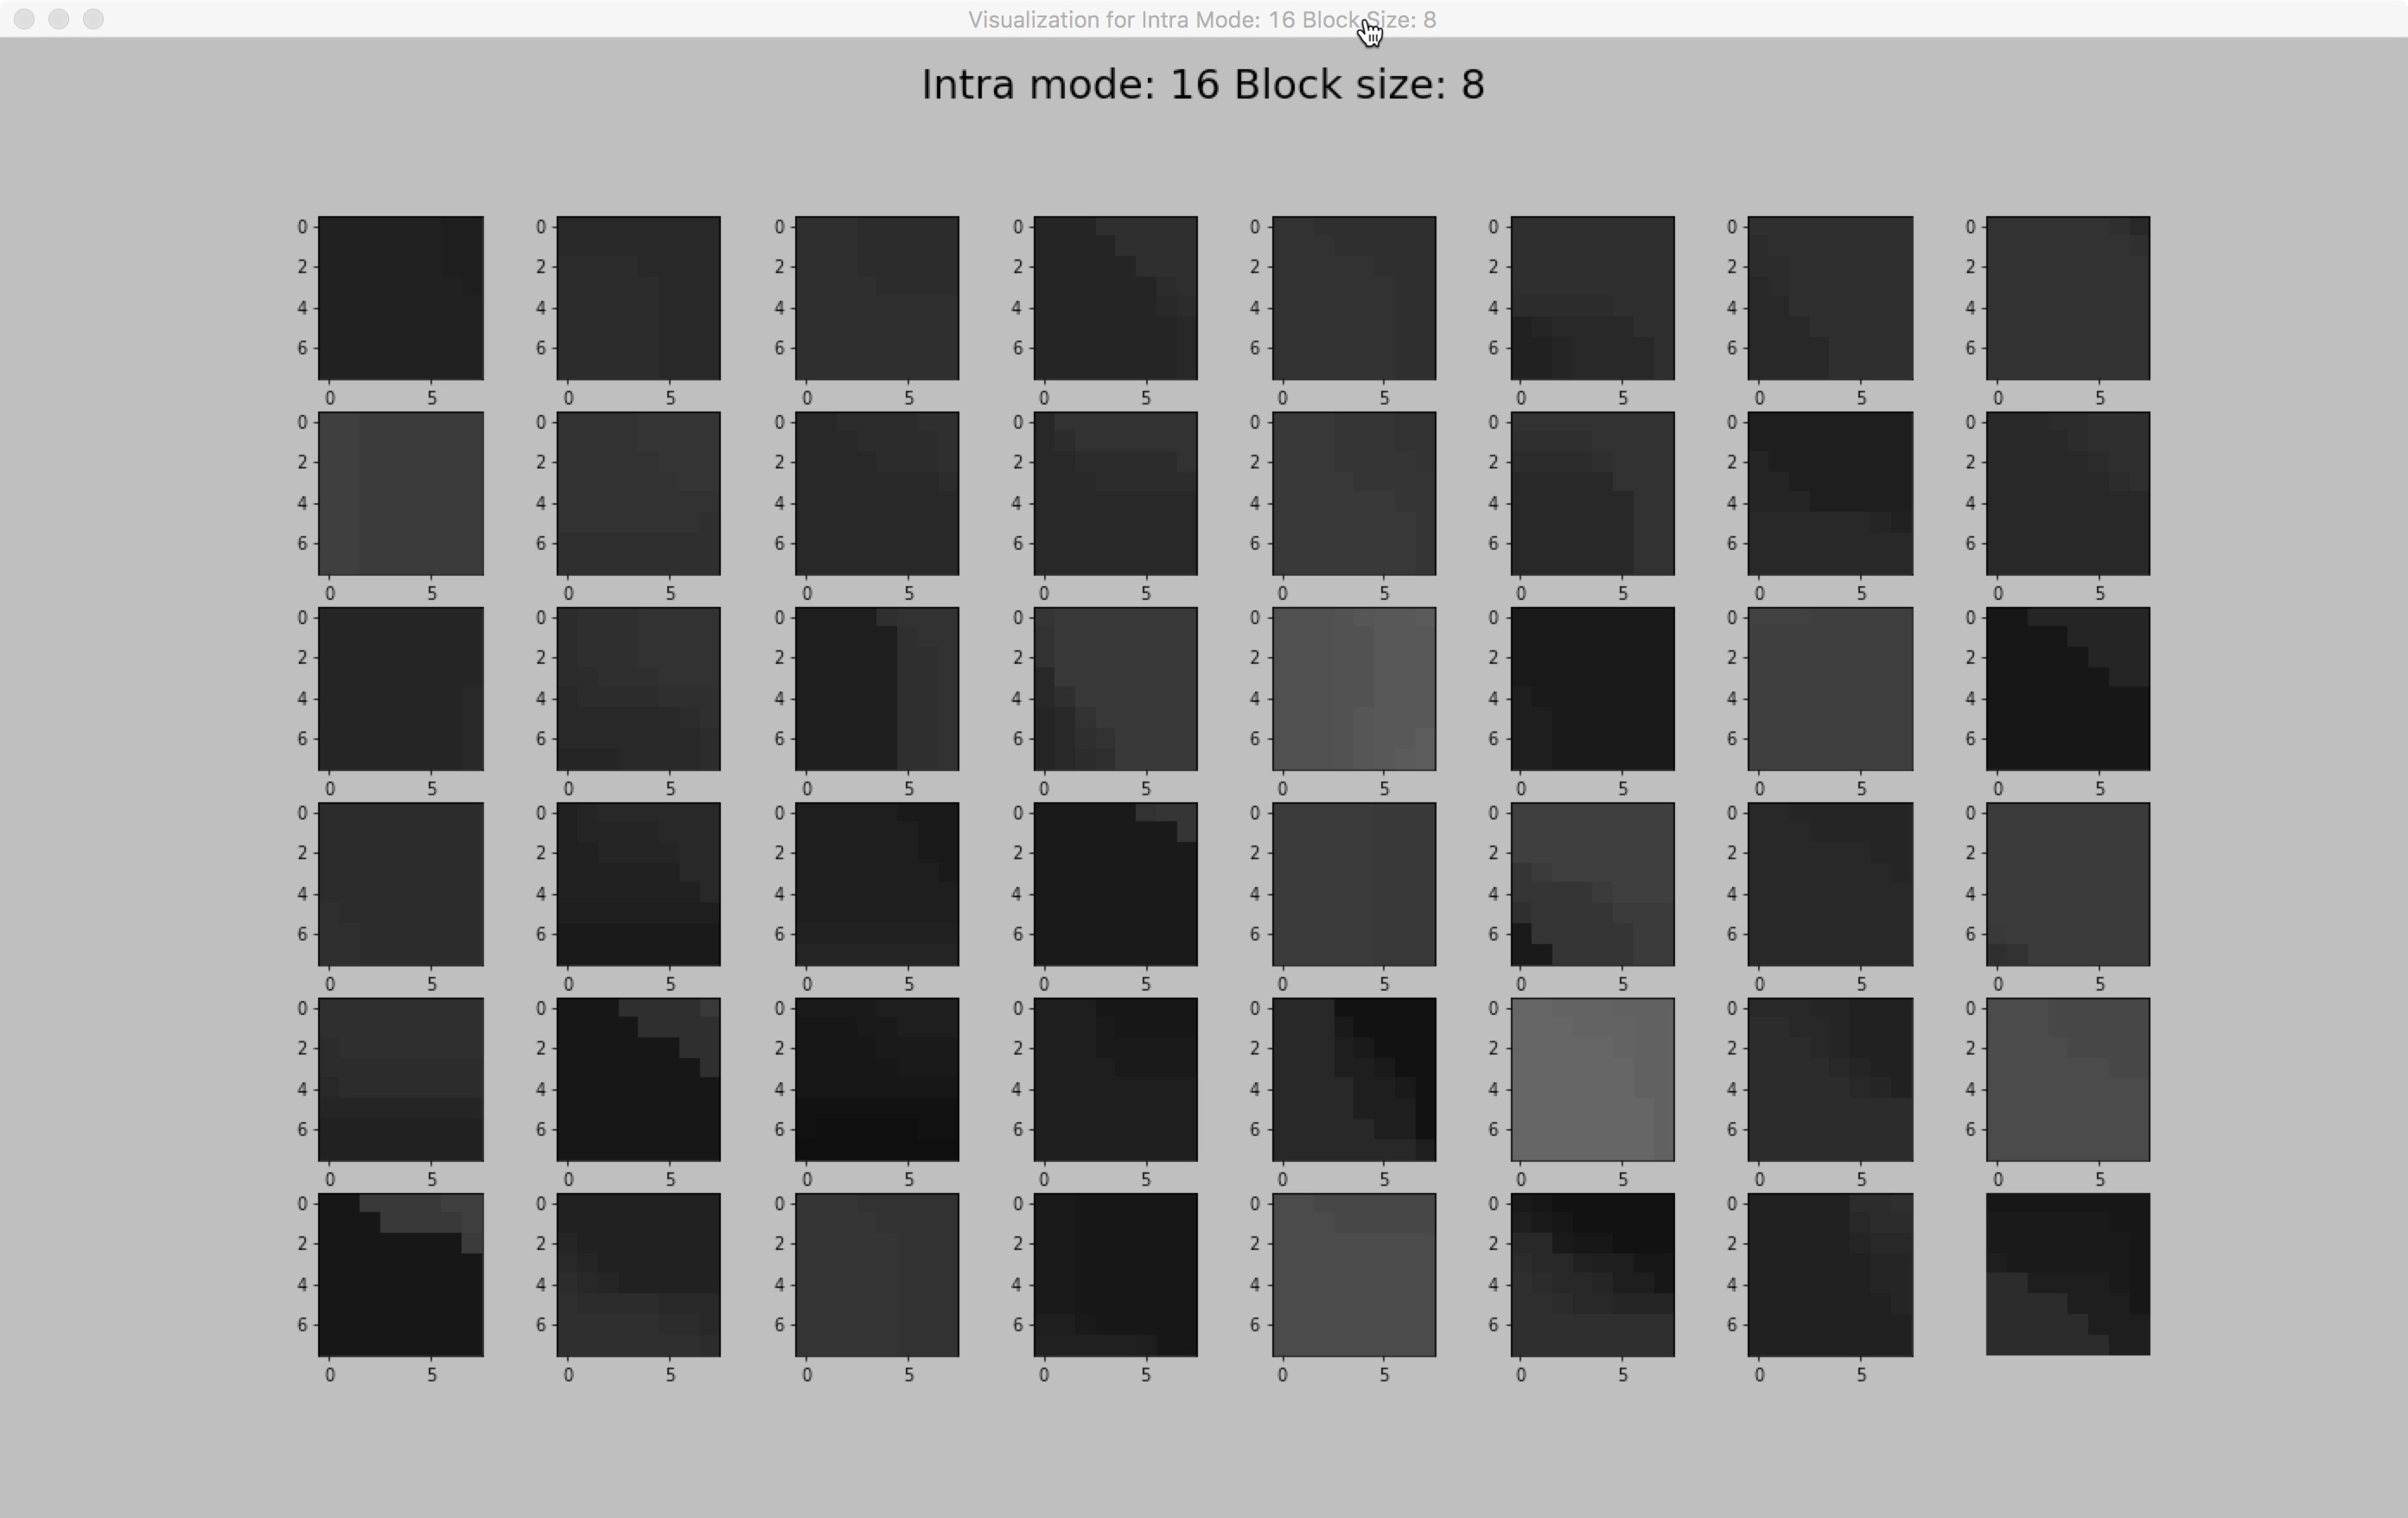
\includegraphics[width=\linewidth]{Figures/visu-size8x8/8-16}
        \caption[Intra mode 16]{intra mode 16.}
        \label{fig:size8_mode16}
    \end{minipage}
    \hspace{\fill} % note: no blank line here
    \begin{minipage}{0.49\textwidth}
        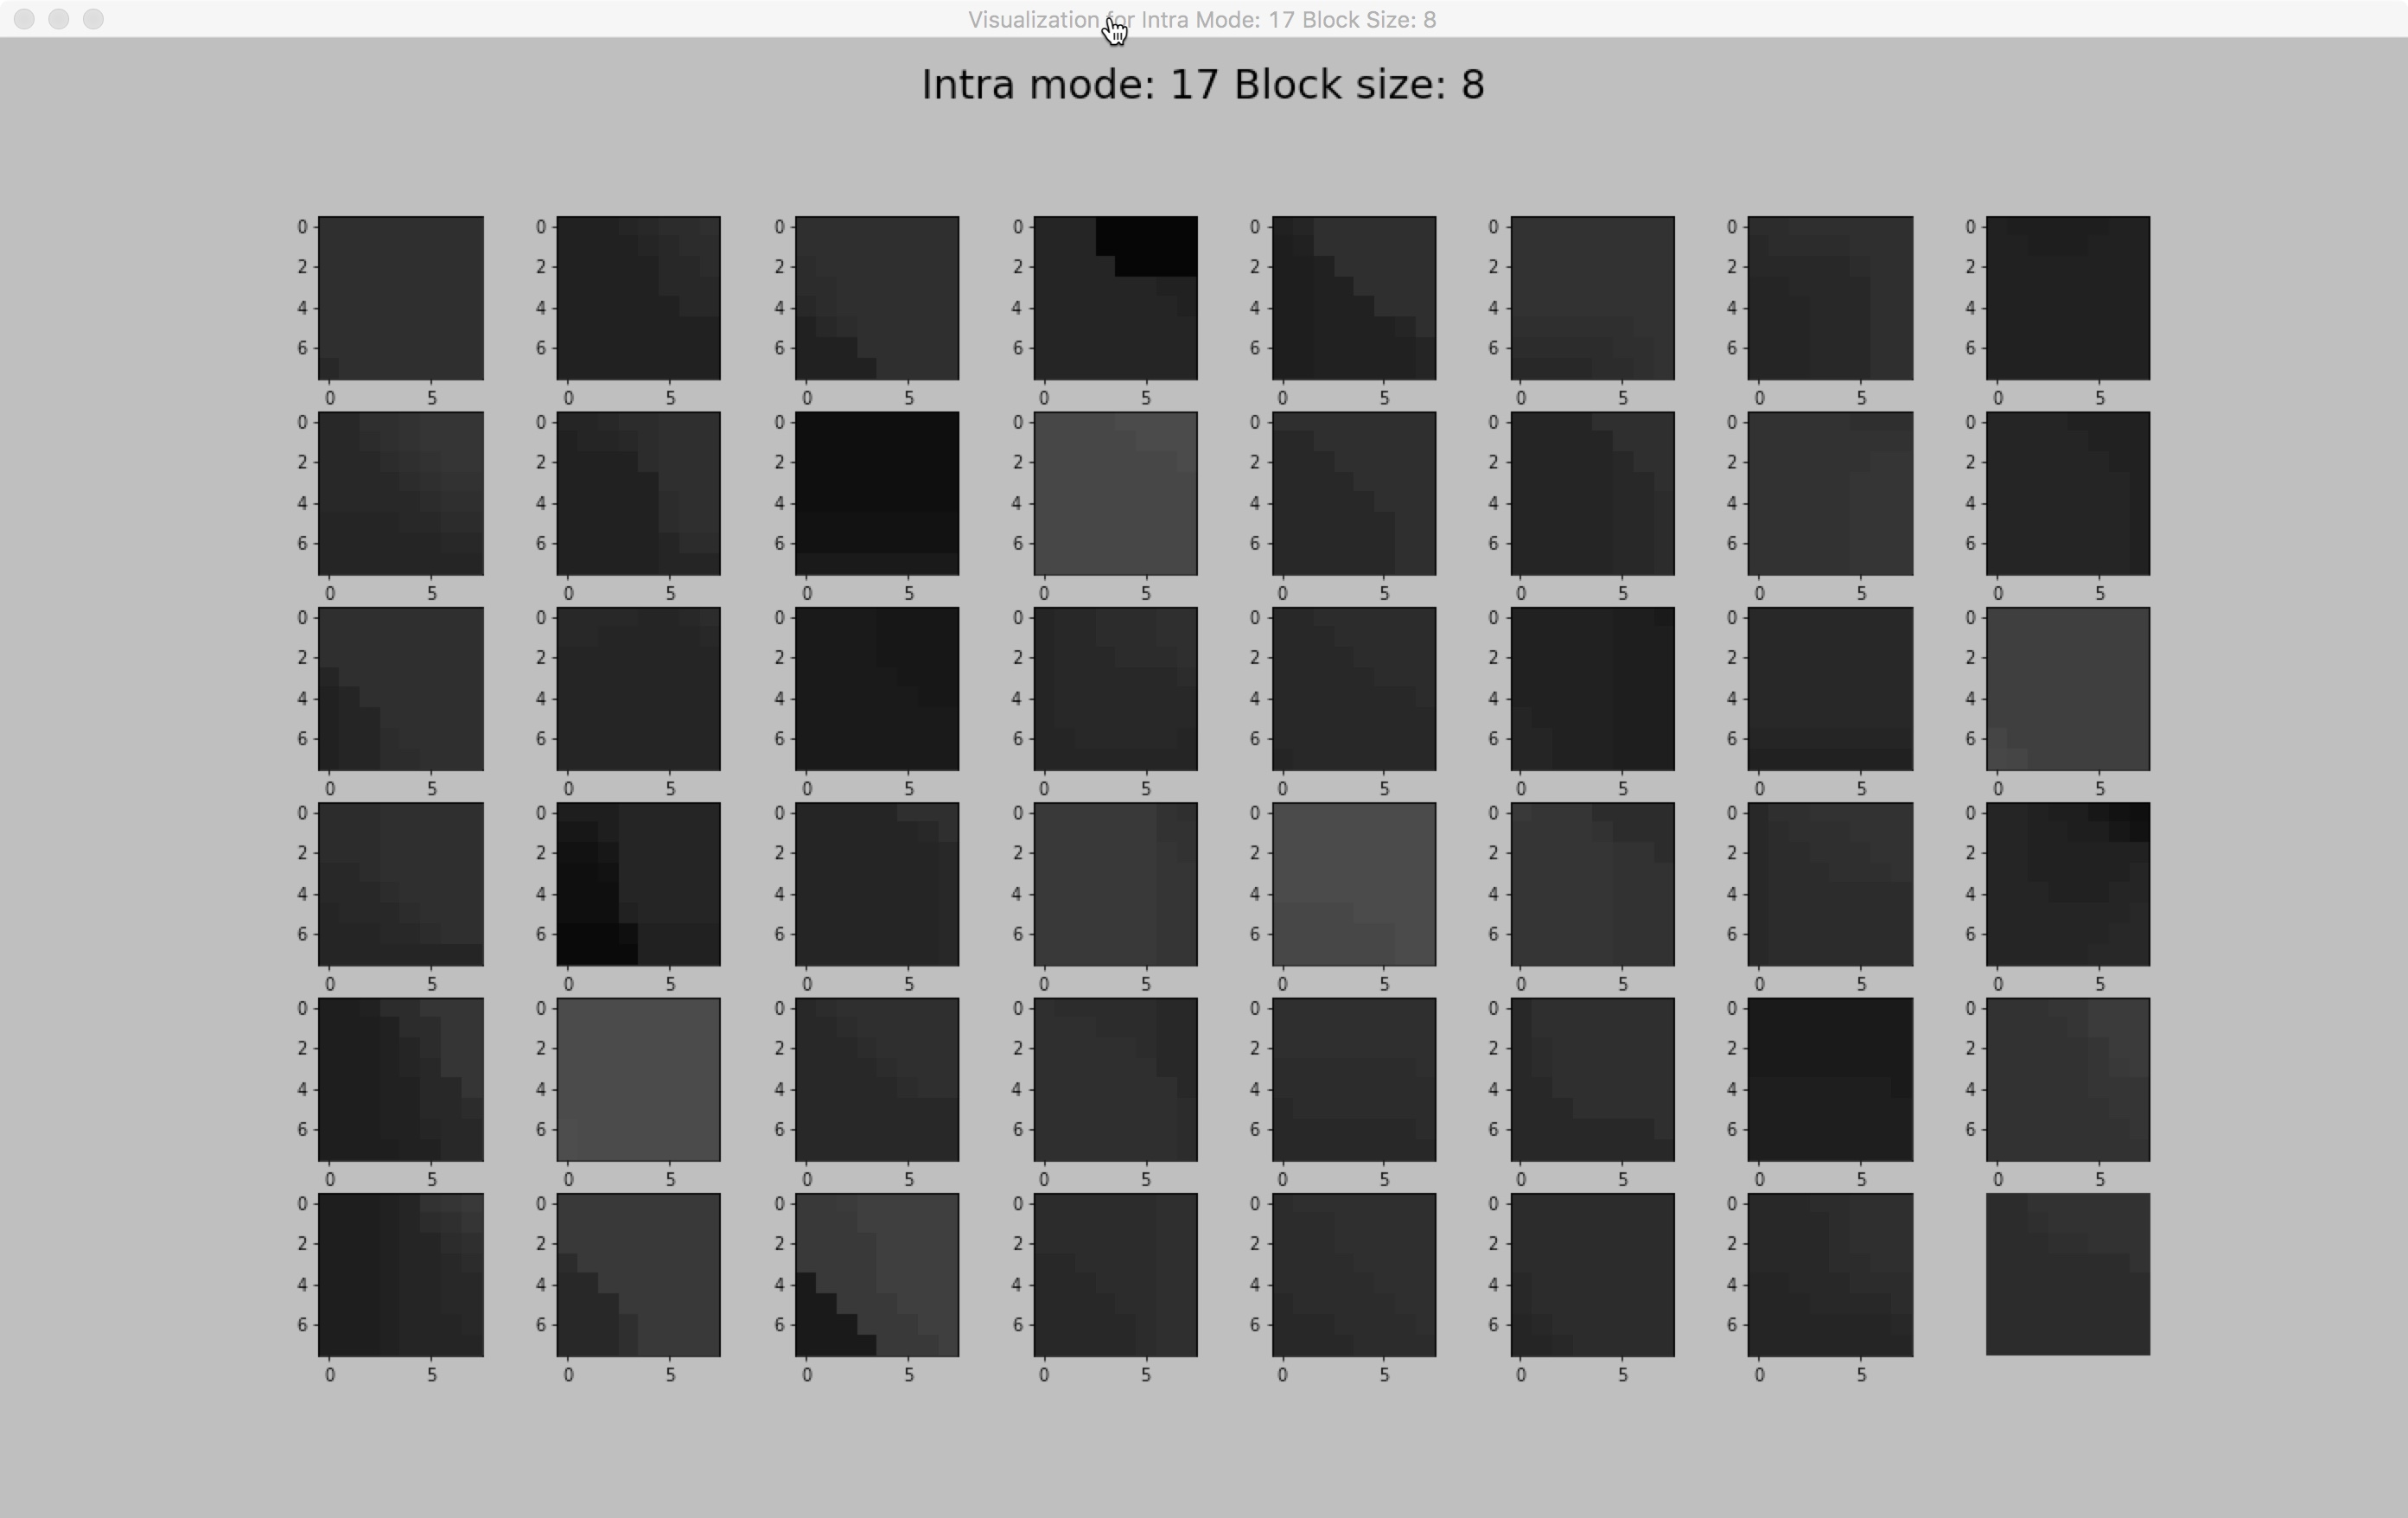
\includegraphics[width=\linewidth]{Figures/visu-size8x8/8-17}
        \caption[Intra mode 17]{intra mode 17.}
        \label{fig:size8_mode17}
    \end{minipage}

    \vspace*{1cm} % vertical separation

    \begin{minipage}{0.49\textwidth}
        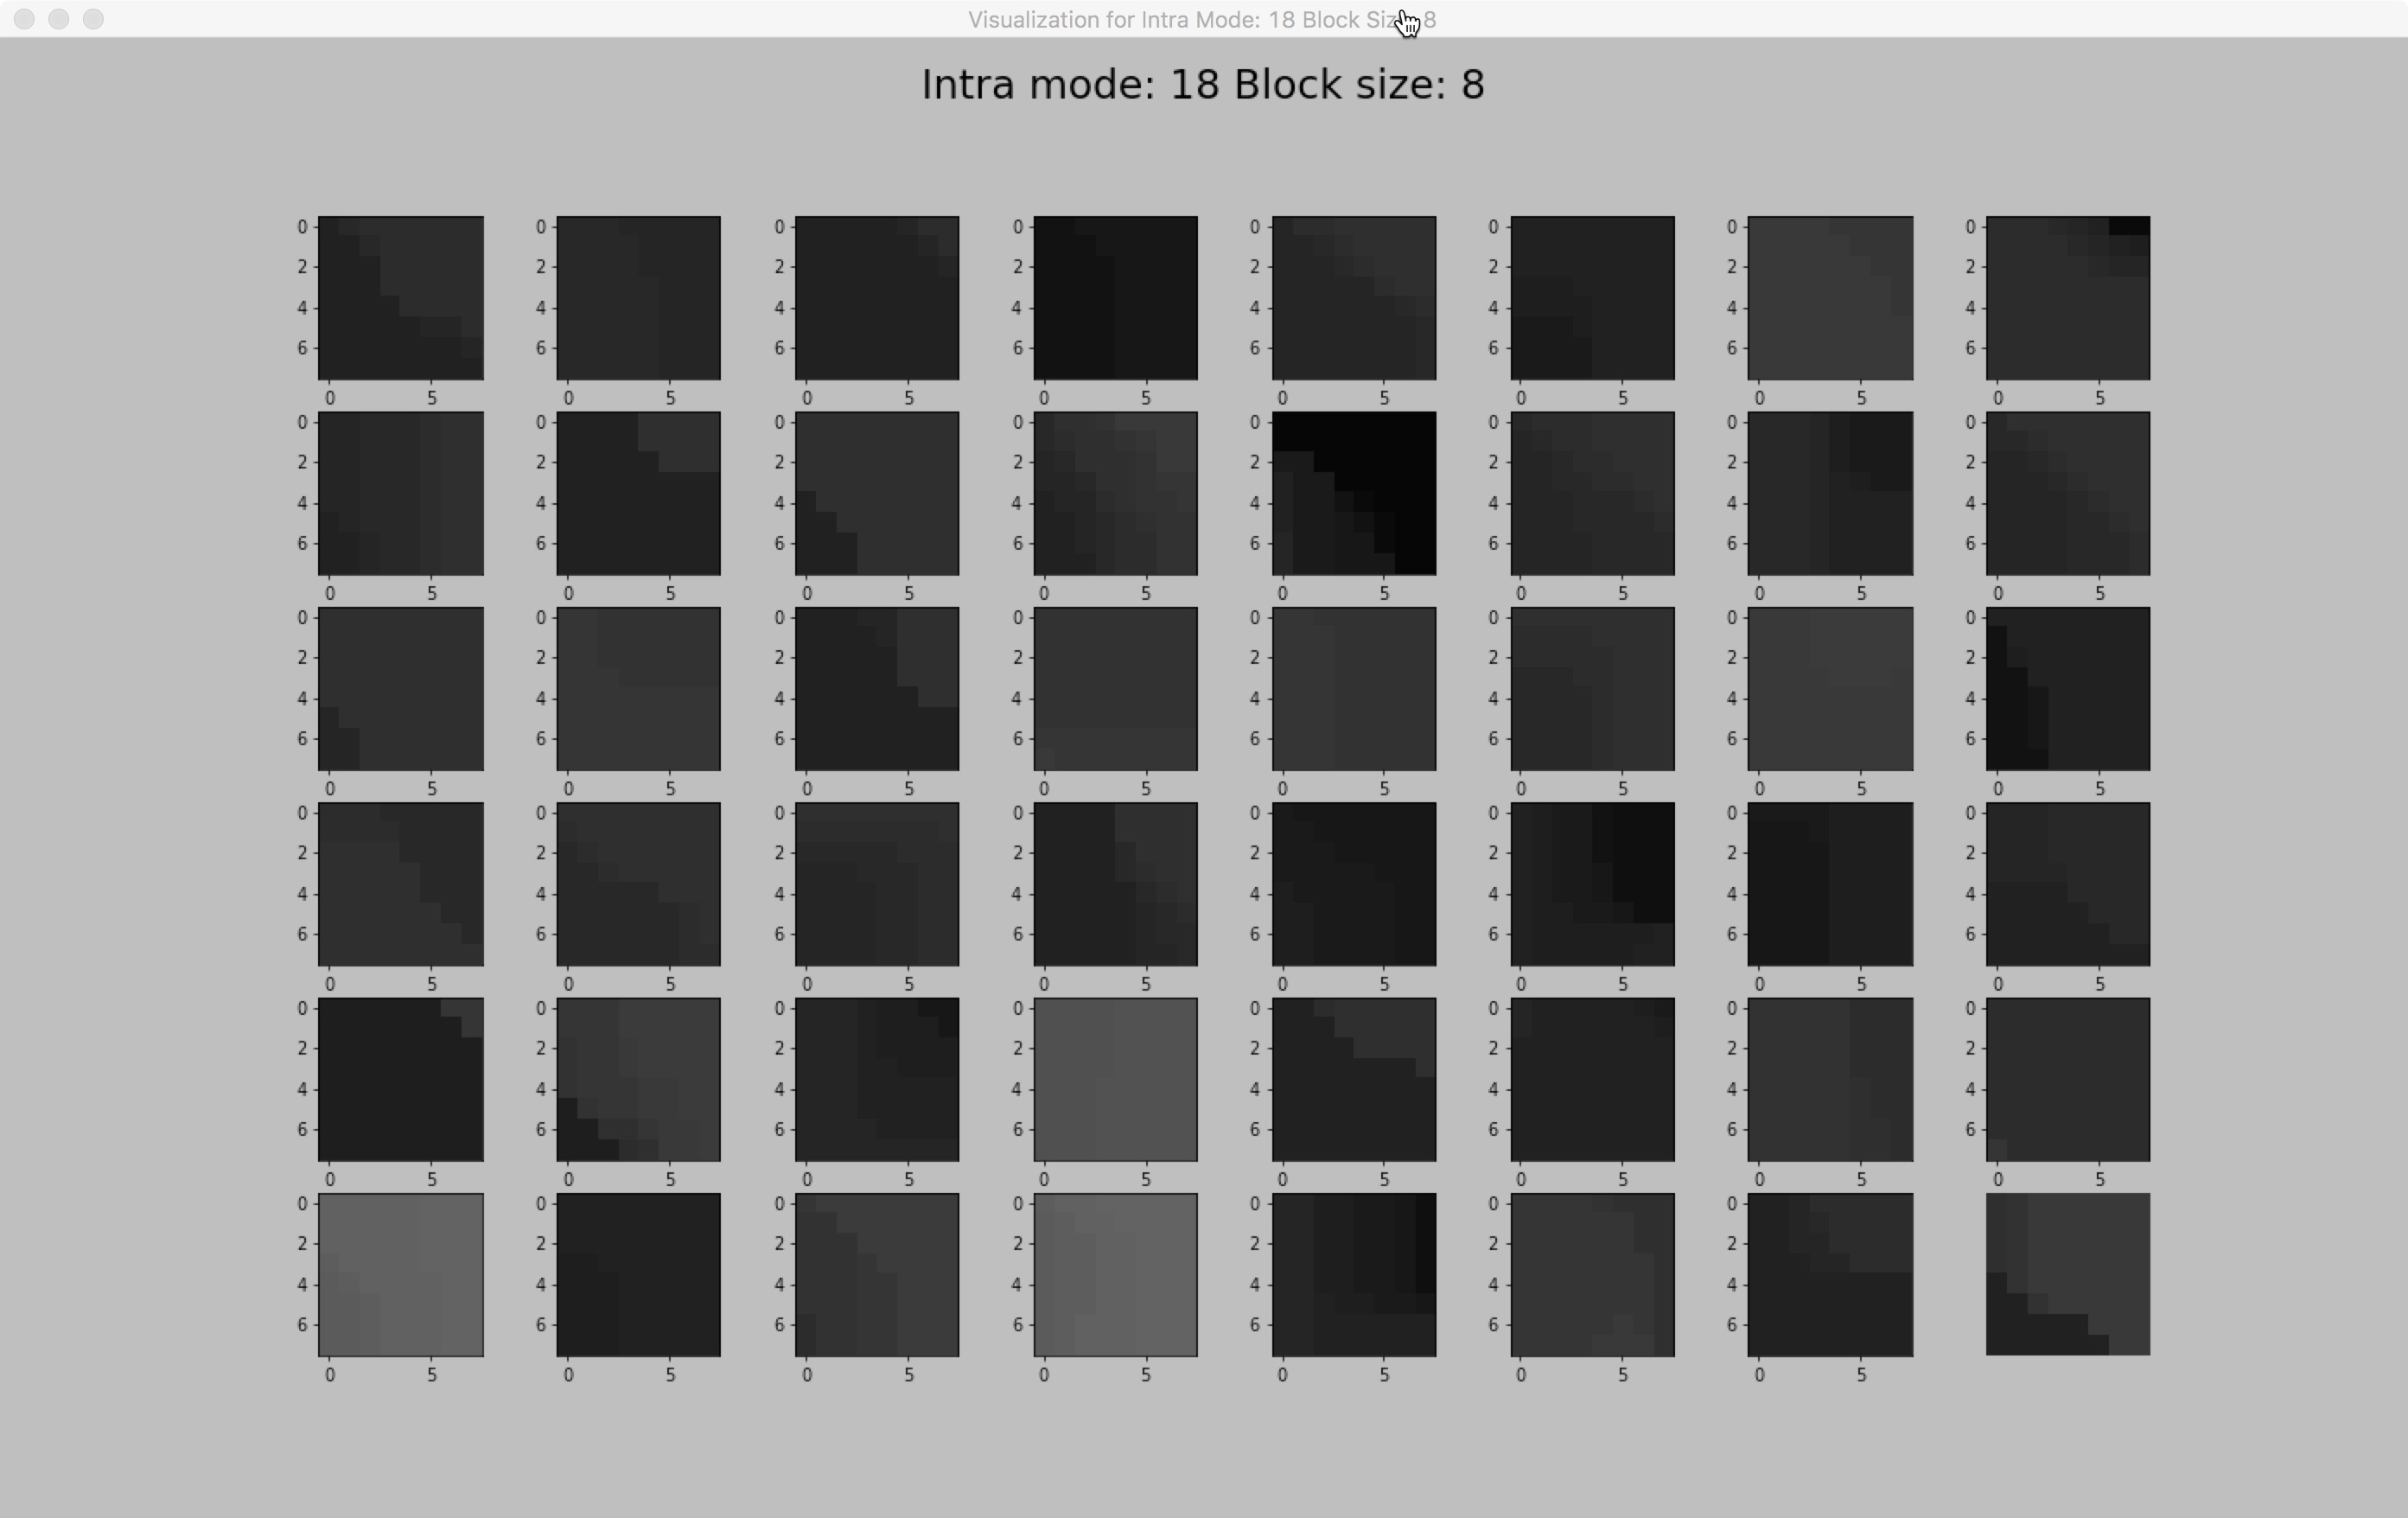
\includegraphics[width=\linewidth]{Figures/visu-size8x8/8-18}
        \caption[Intra mode 18]{intra mode 18.}
        \label{fig:size8_mode18}
    \end{minipage}
    \hspace{\fill} % note: no blank line here
    \begin{minipage}{0.49\textwidth}
        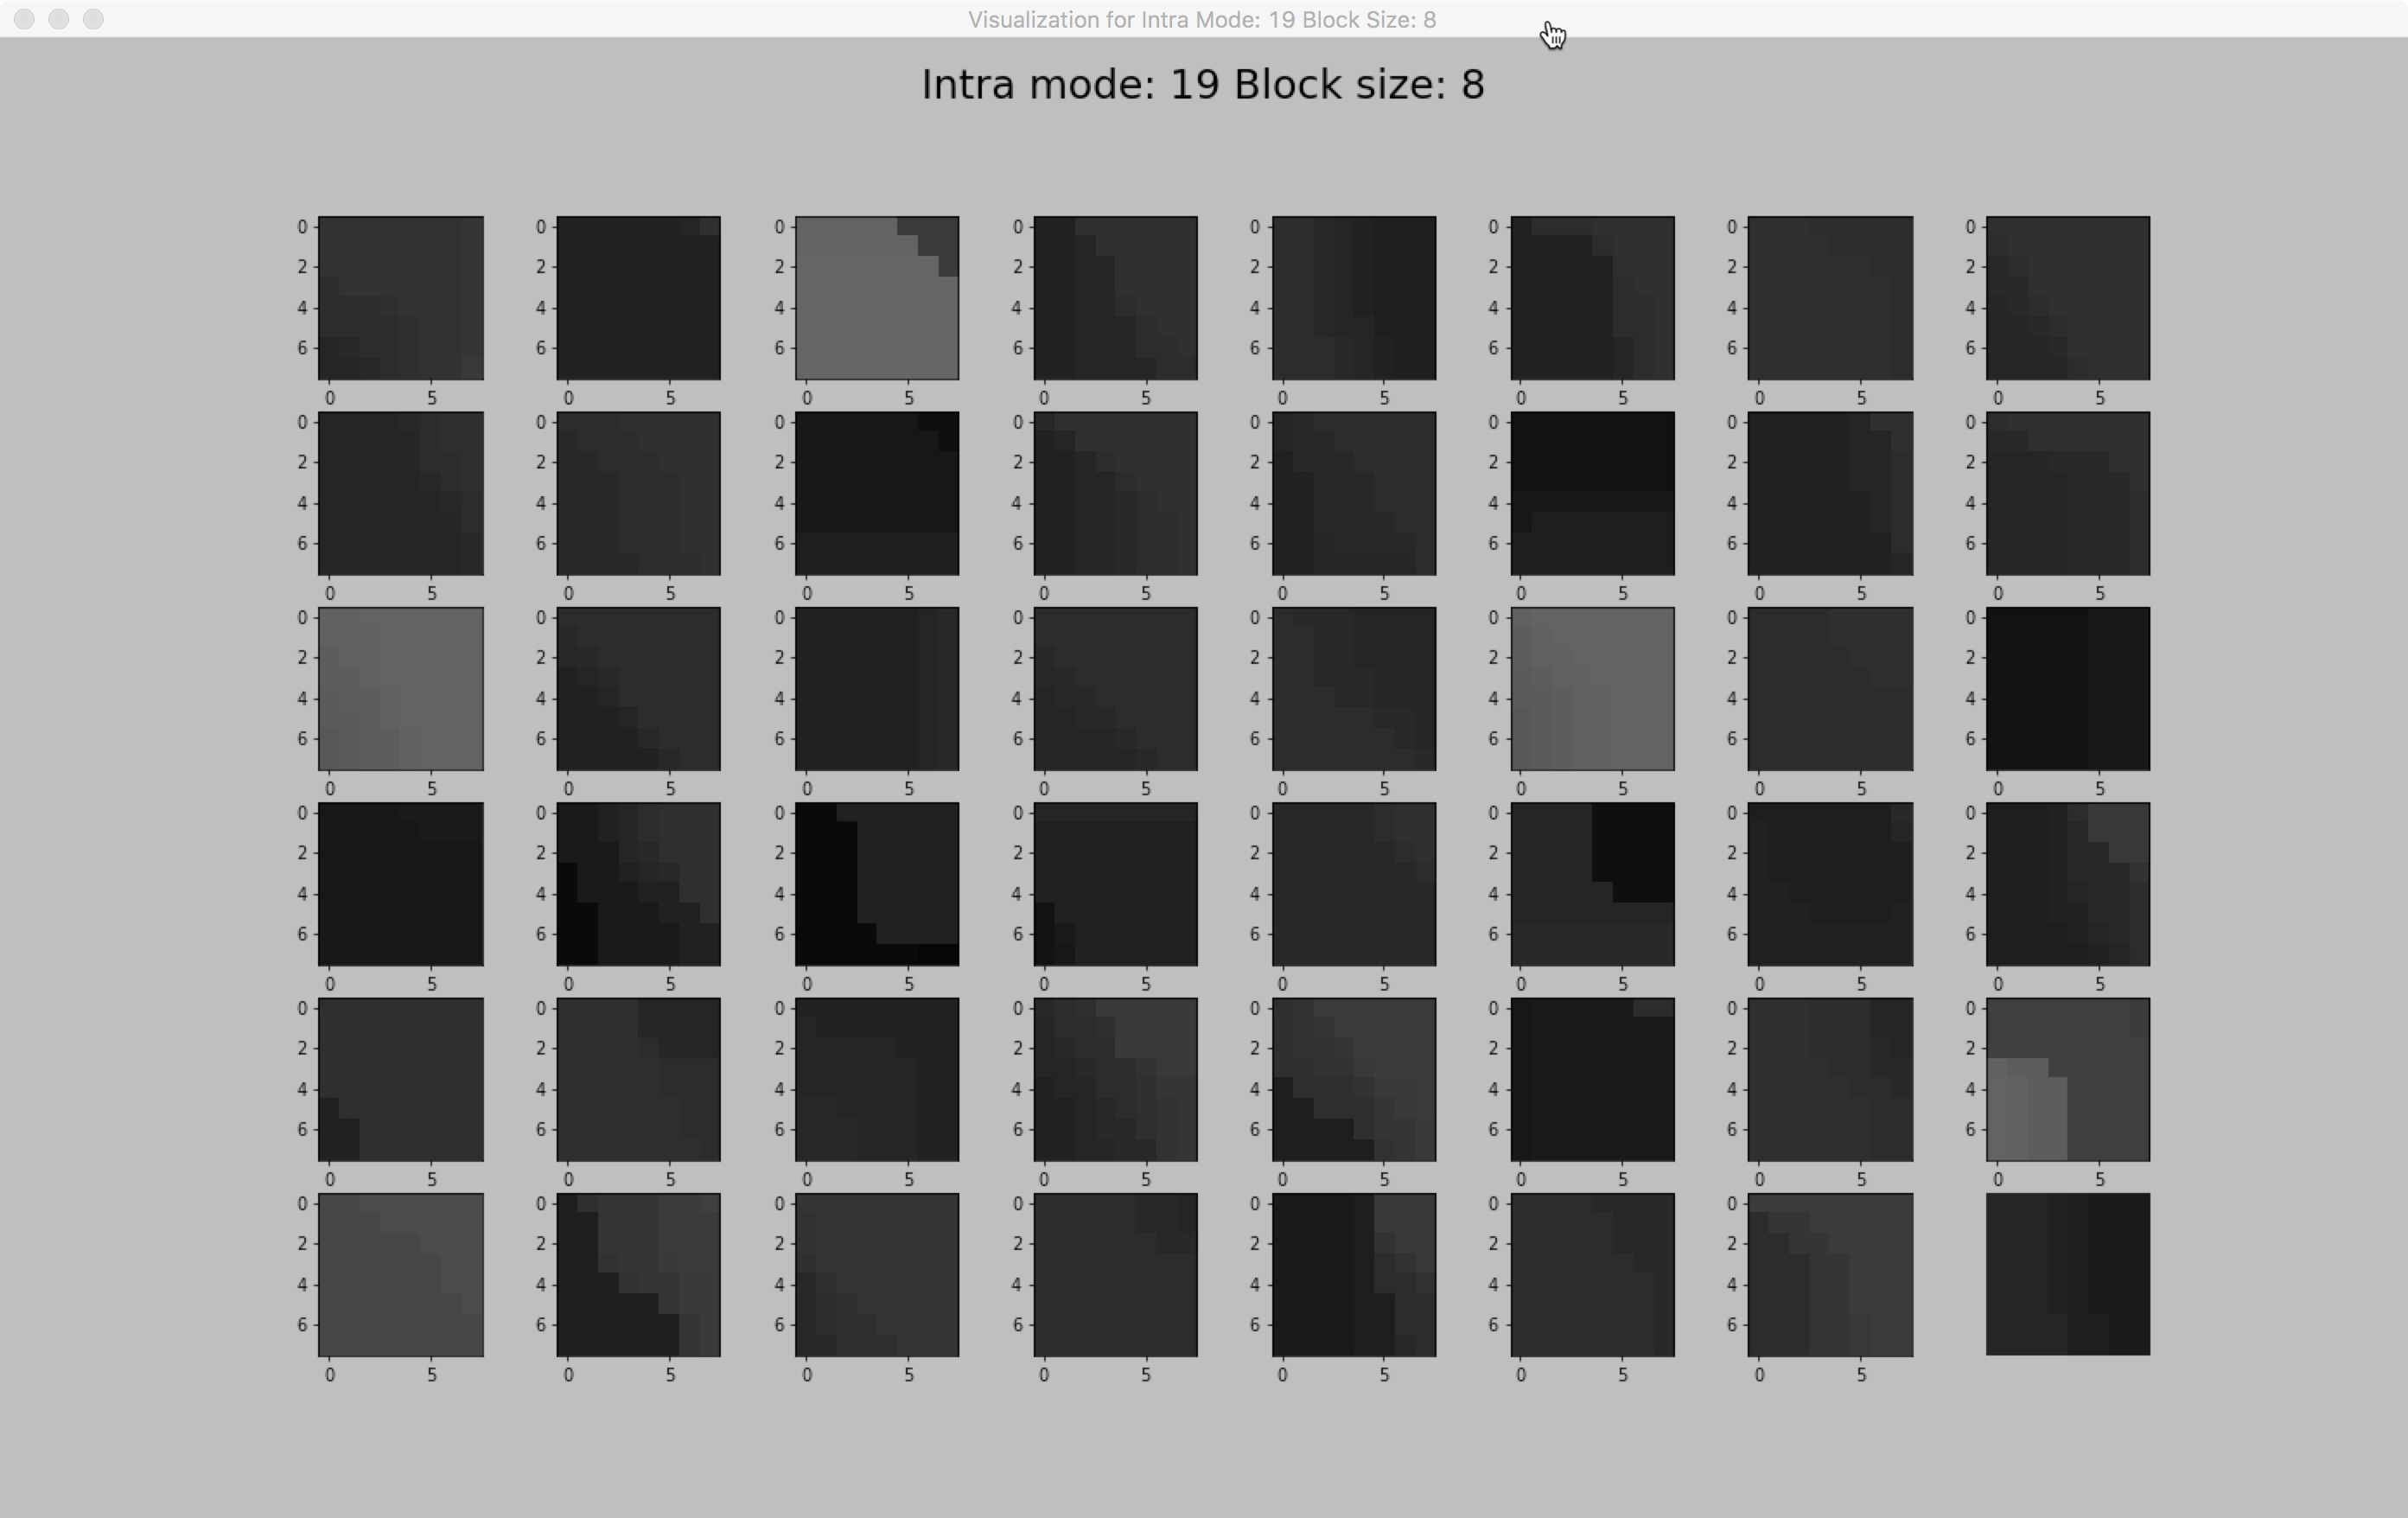
\includegraphics[width=\linewidth]{Figures/visu-size8x8/8-19}
        \caption[Intra mode 19]{intra mode 19.}
        \label{fig:size8_mode19}
    \end{minipage}
    
    \vspace*{1cm} % vertical separation

    \begin{minipage}{0.49\textwidth}
        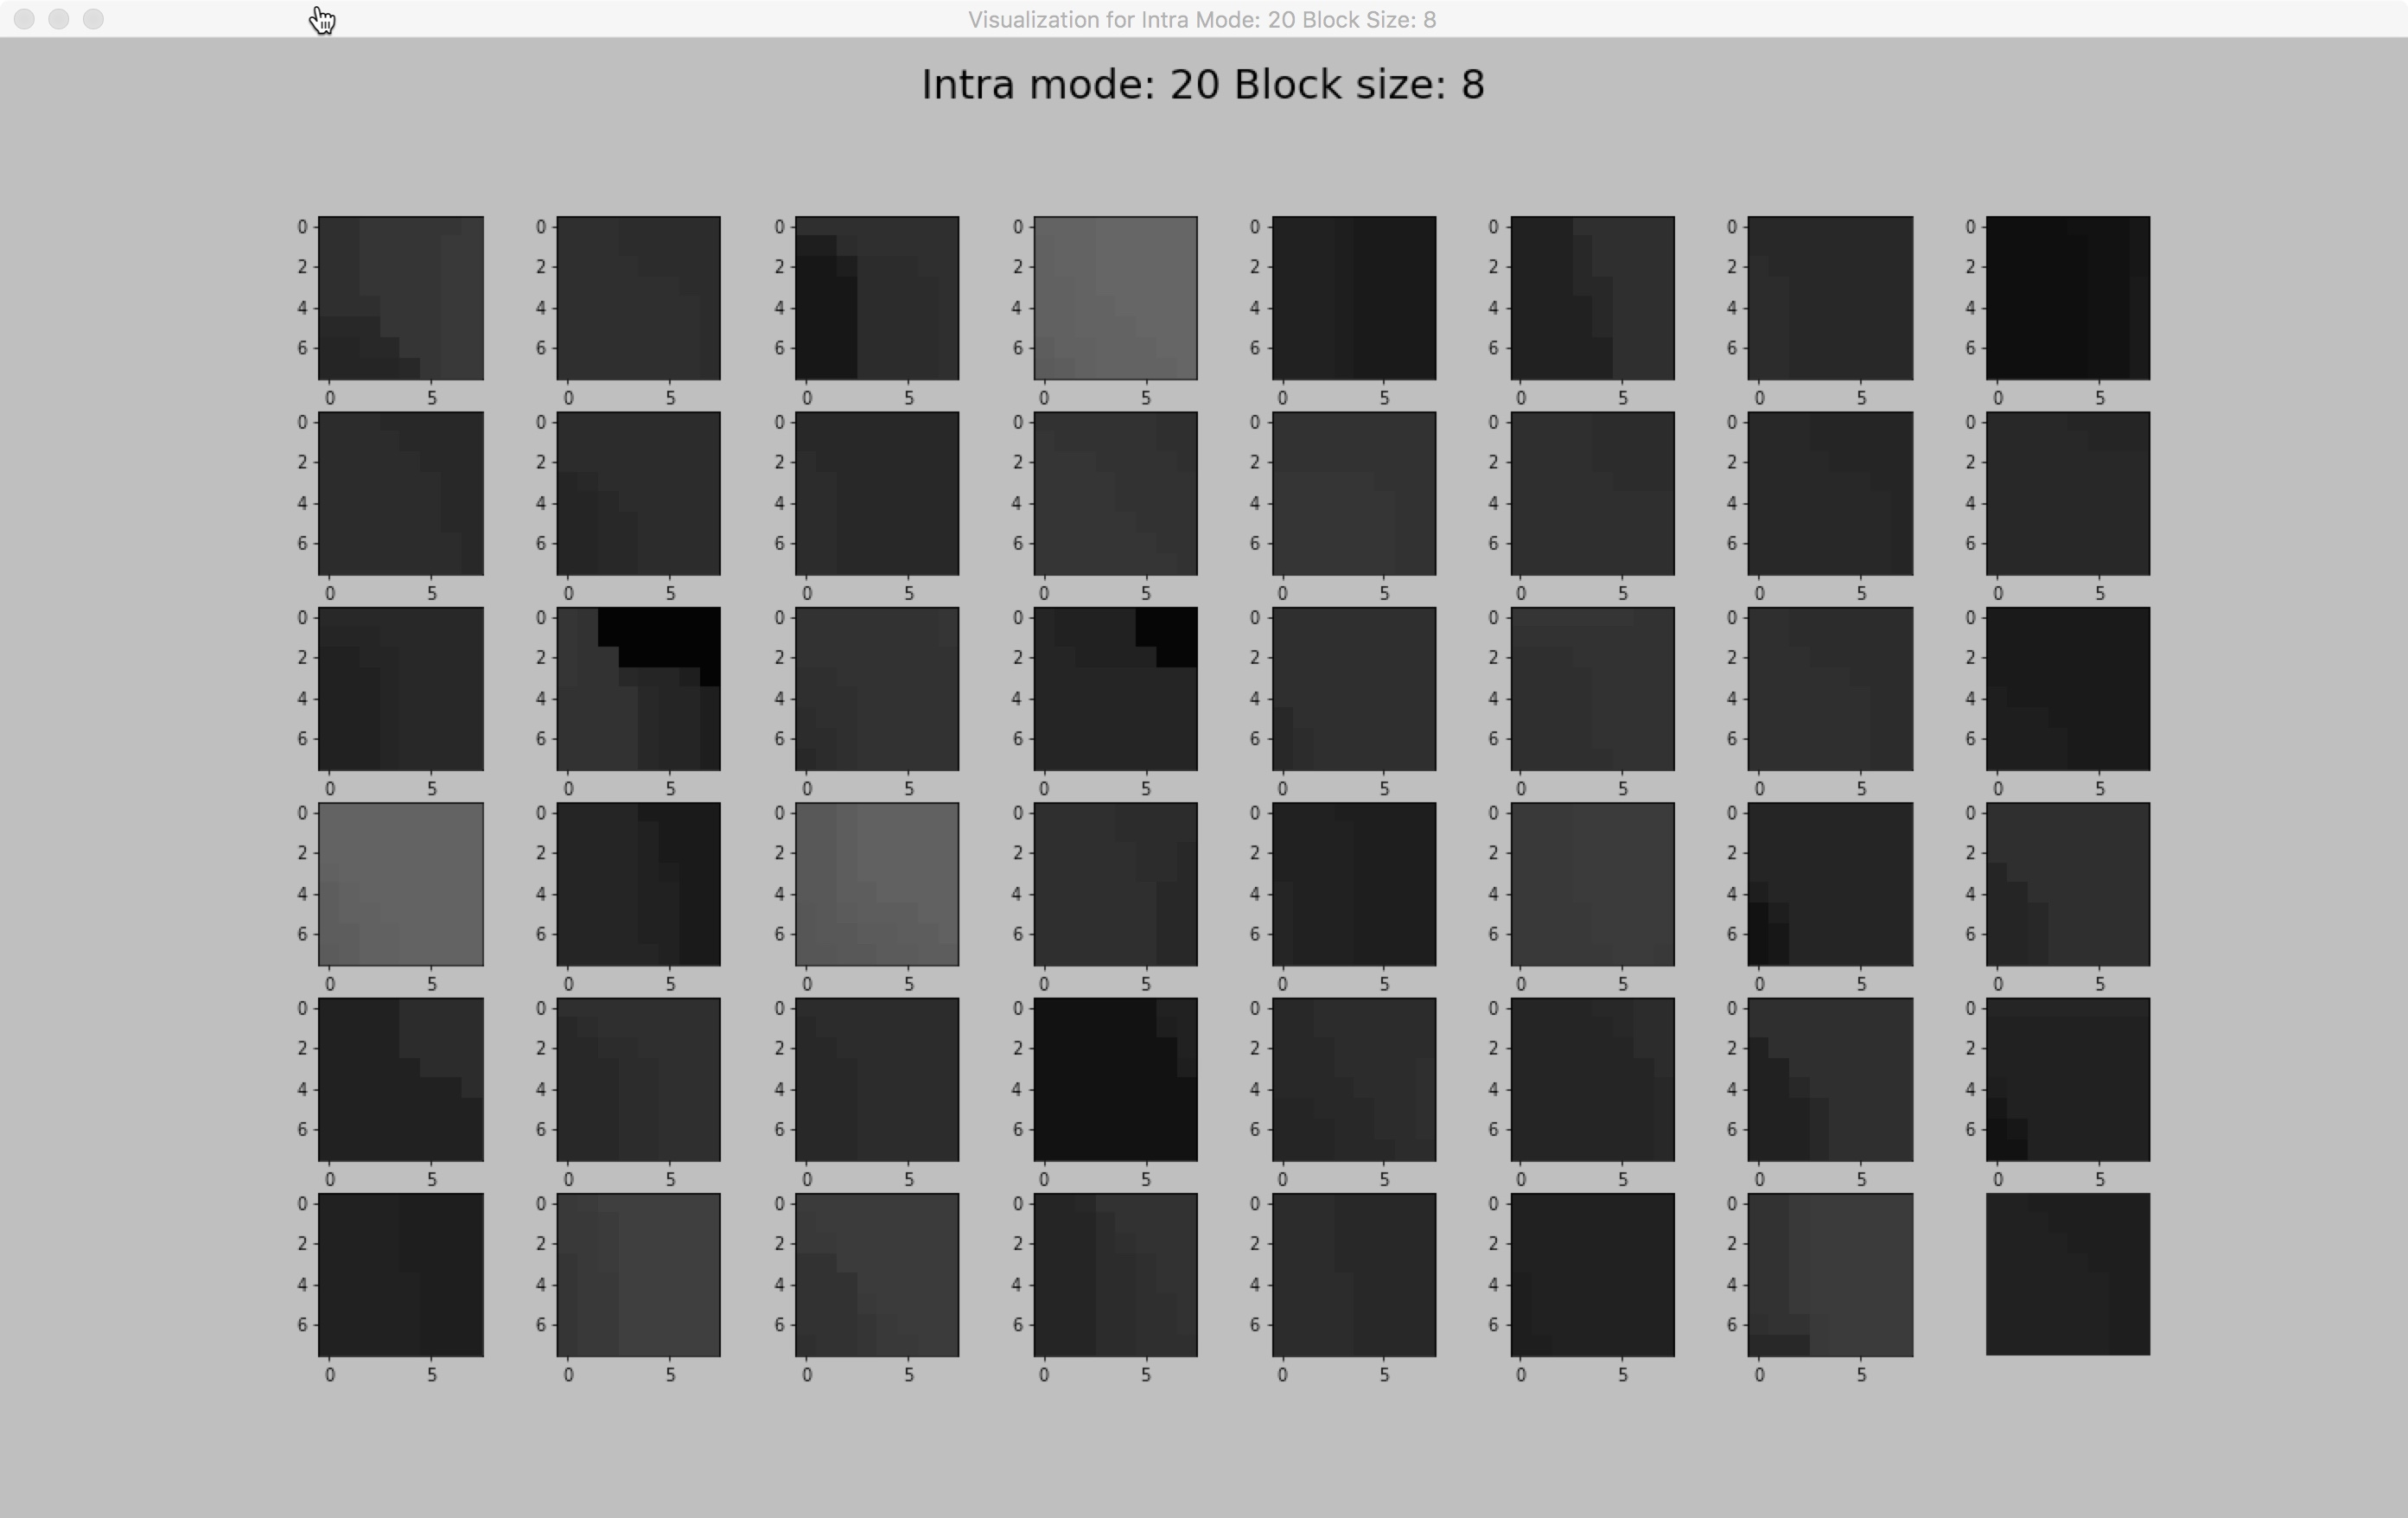
\includegraphics[width=\linewidth]{Figures/visu-size8x8/8-20}
        \caption[Intra mode 20]{intra mode 20.}
        \label{fig:size8_mode20}
    \end{minipage}
    \hspace{\fill} % note: no blank line here
    \begin{minipage}{0.49\textwidth}
        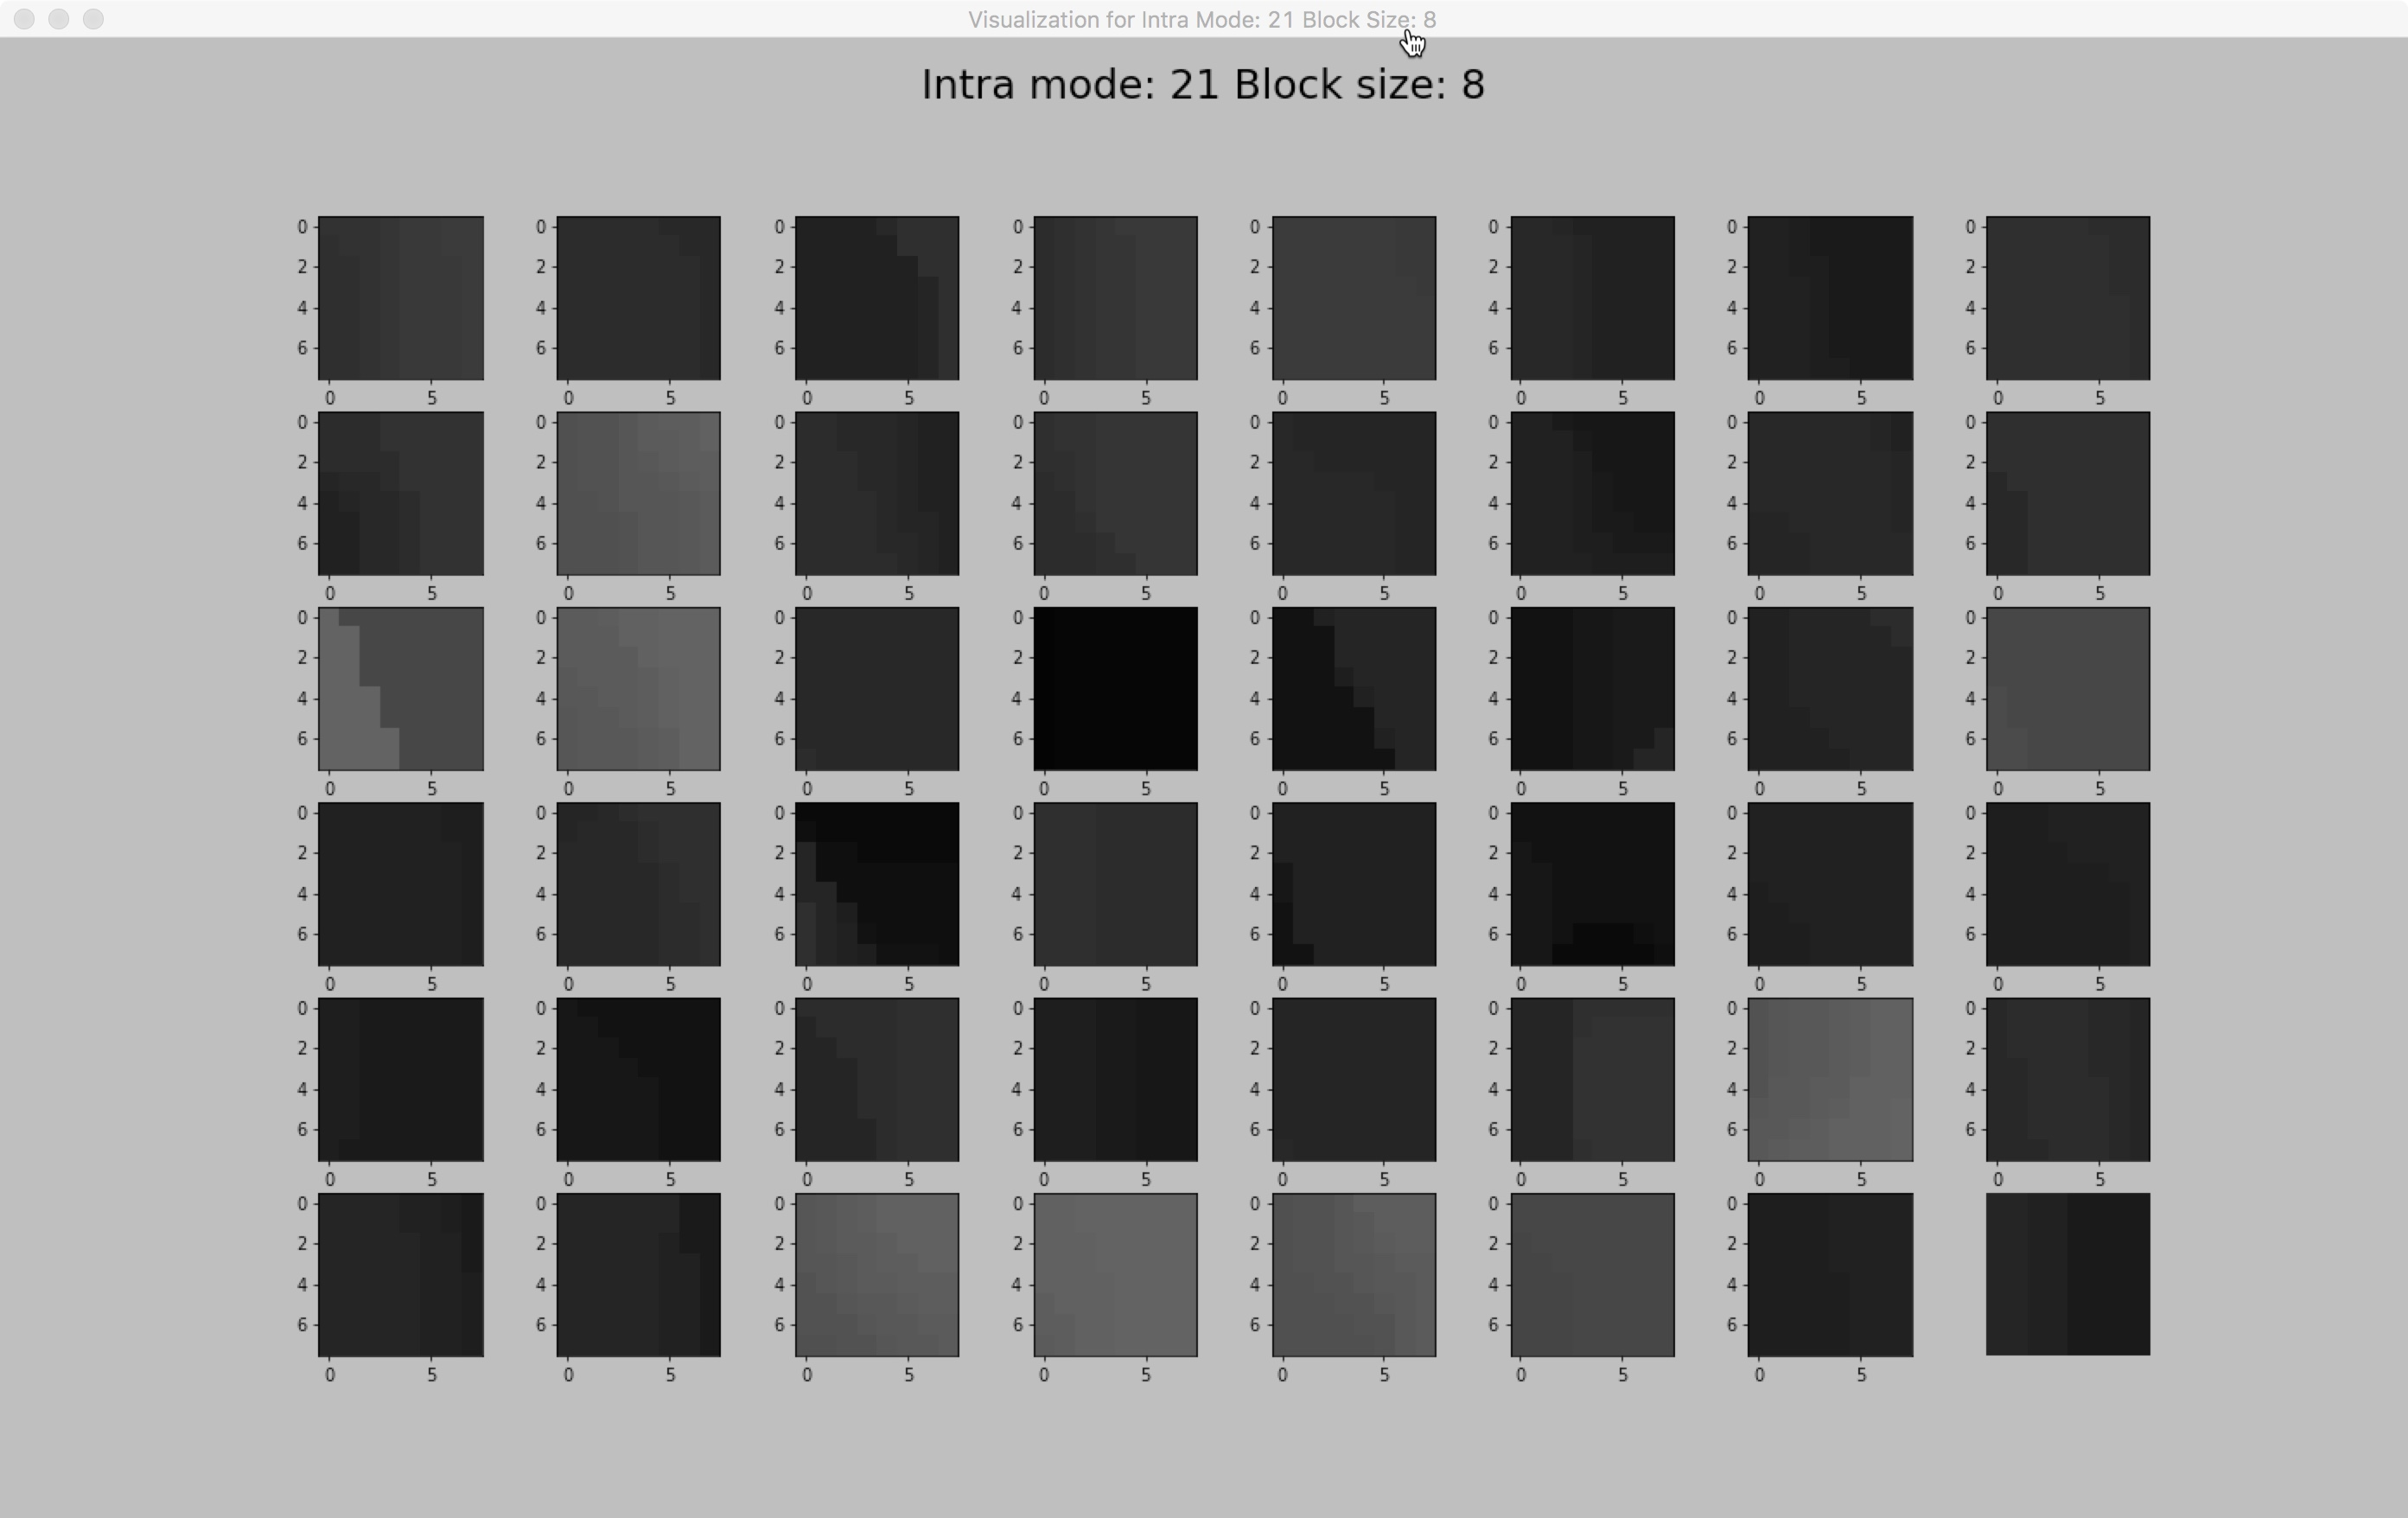
\includegraphics[width=\linewidth]{Figures/visu-size8x8/8-21}
        \caption[Intra mode 21]{intra mode 21.}
        \label{fig:size8_mode21}
    \end{minipage}

% \caption{Figure caption goes here}\label{fig:visualizations-for-blocks-of-size8x8-01}
\end{figure}

\begin{figure}[H]

    \vspace*{1cm} % vertical separation

    \begin{minipage}{0.49\textwidth}
        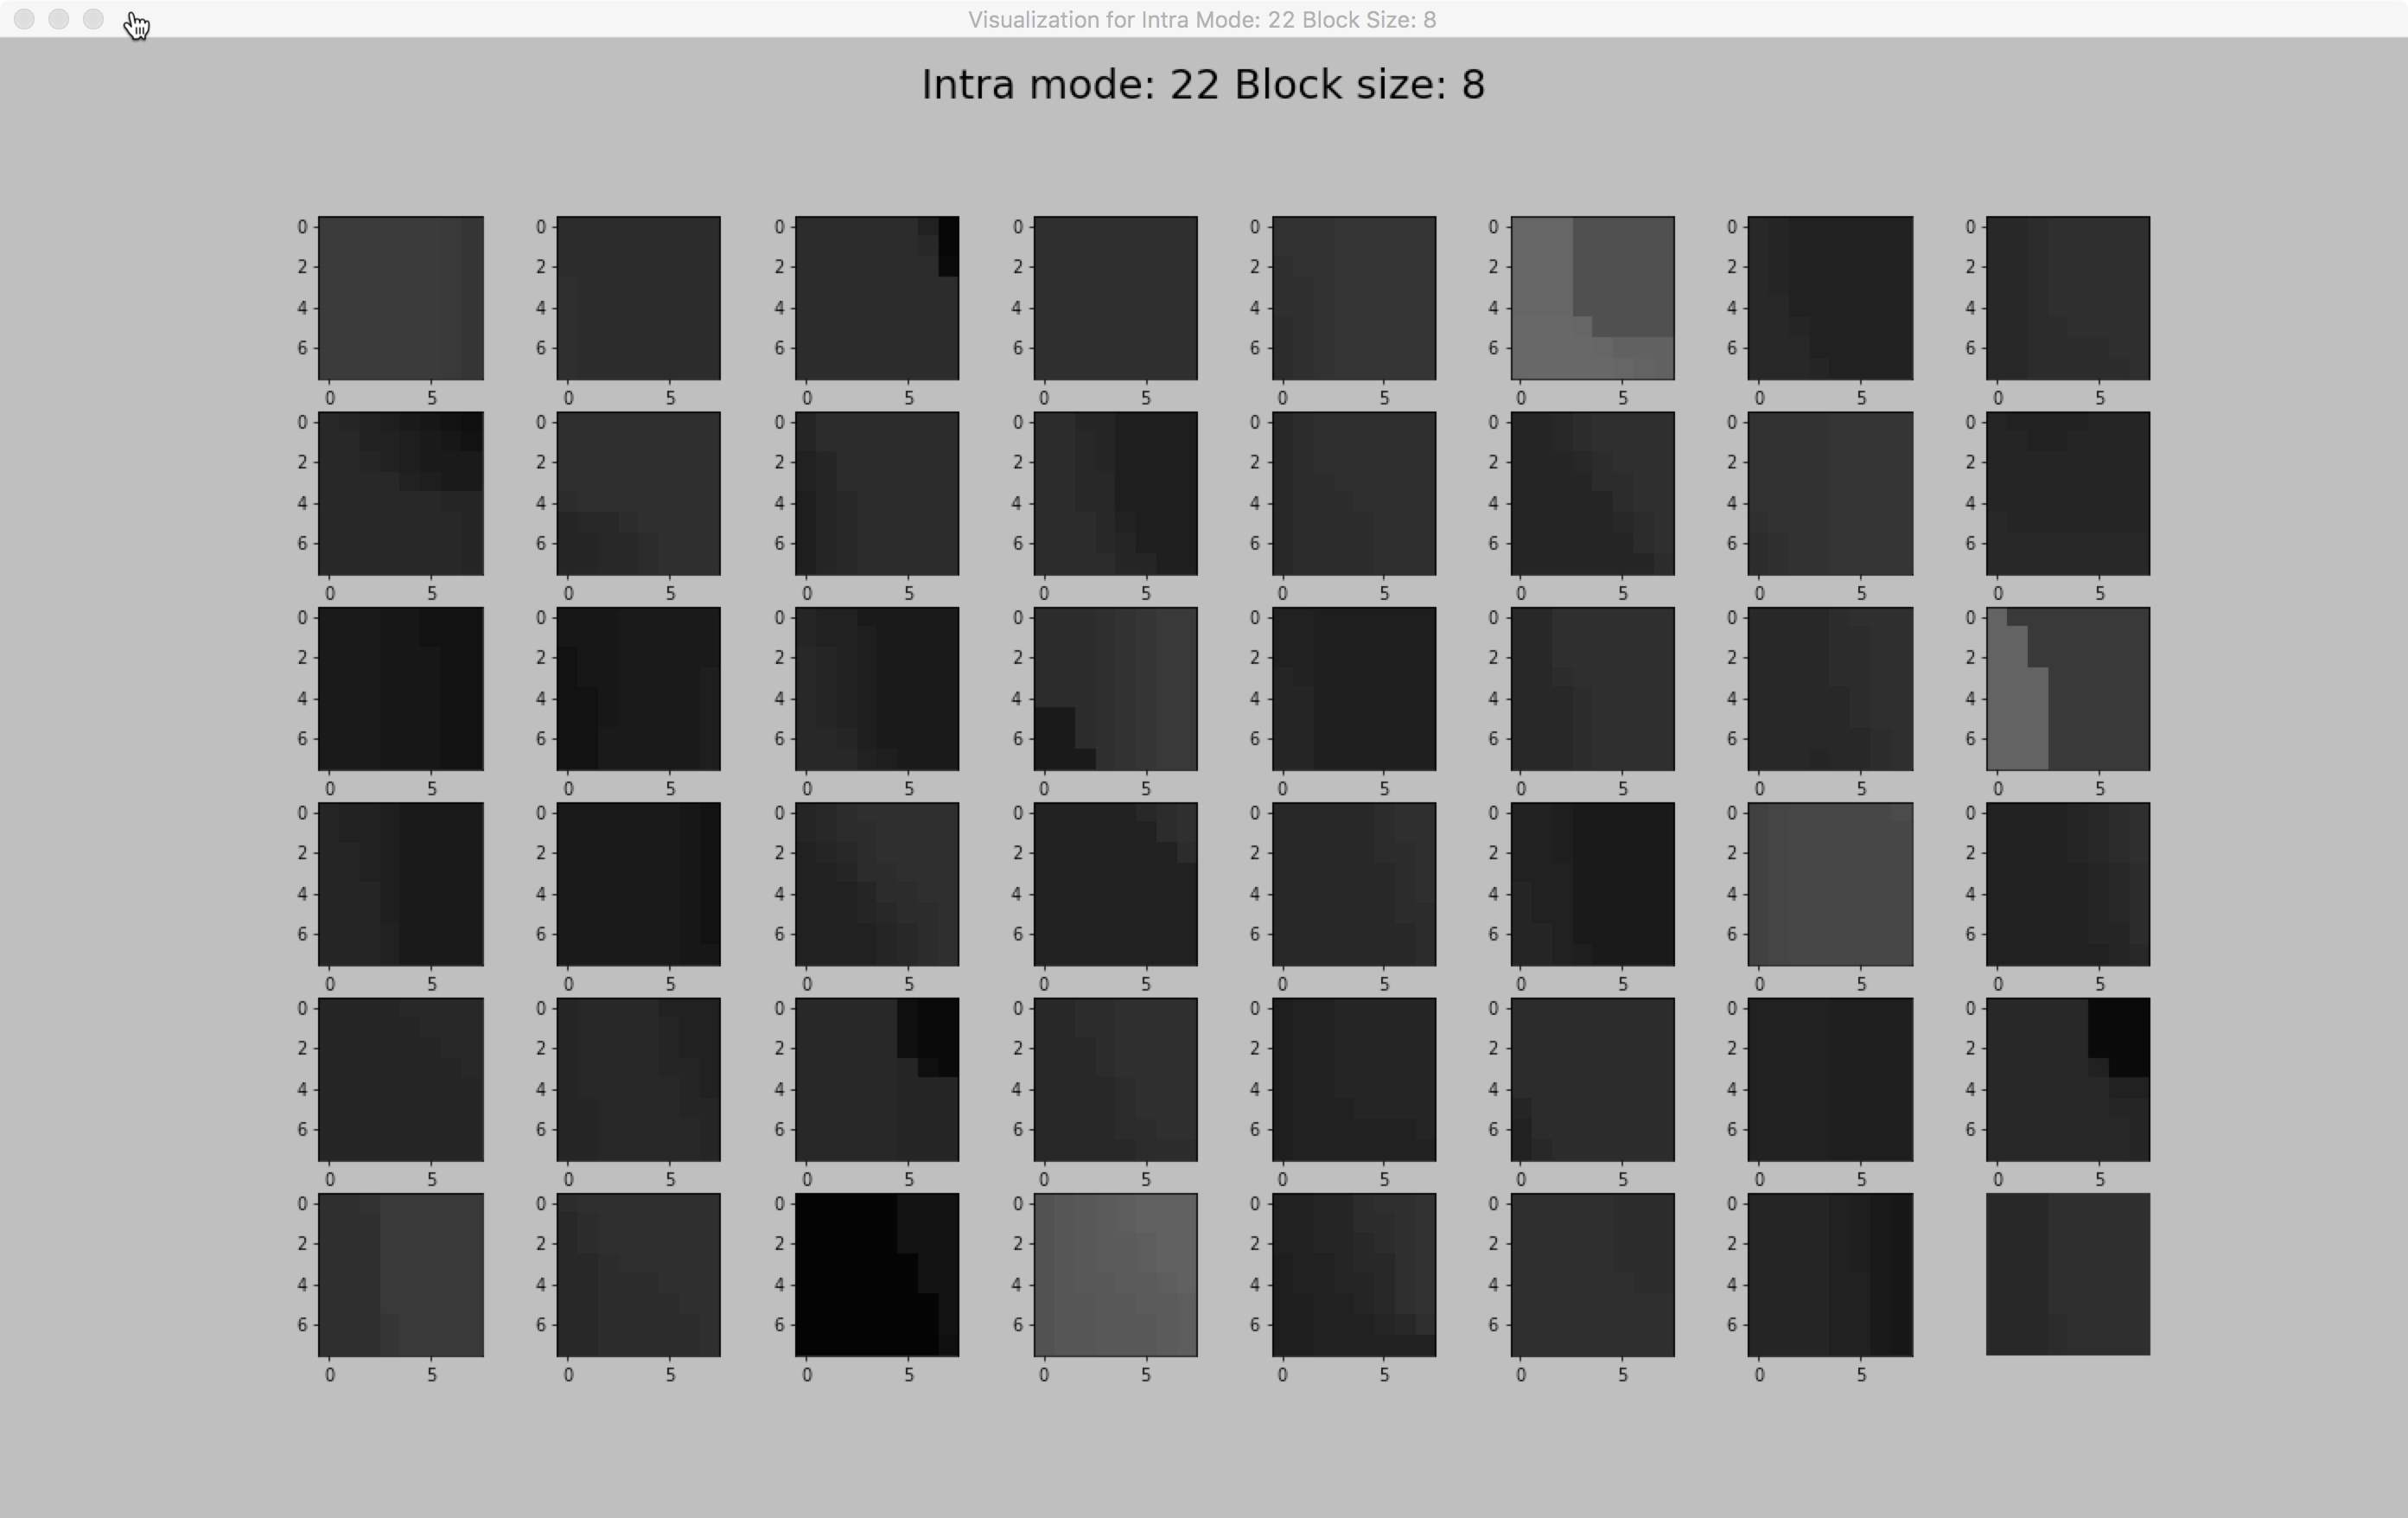
\includegraphics[width=\linewidth]{Figures/visu-size8x8/8-22}
        \caption[Intra mode 22]{intra mode 22.}
        \label{fig:size8_mode22}
    \end{minipage}
    \hspace{\fill} % note: no blank line here
    \begin{minipage}{0.49\textwidth}
        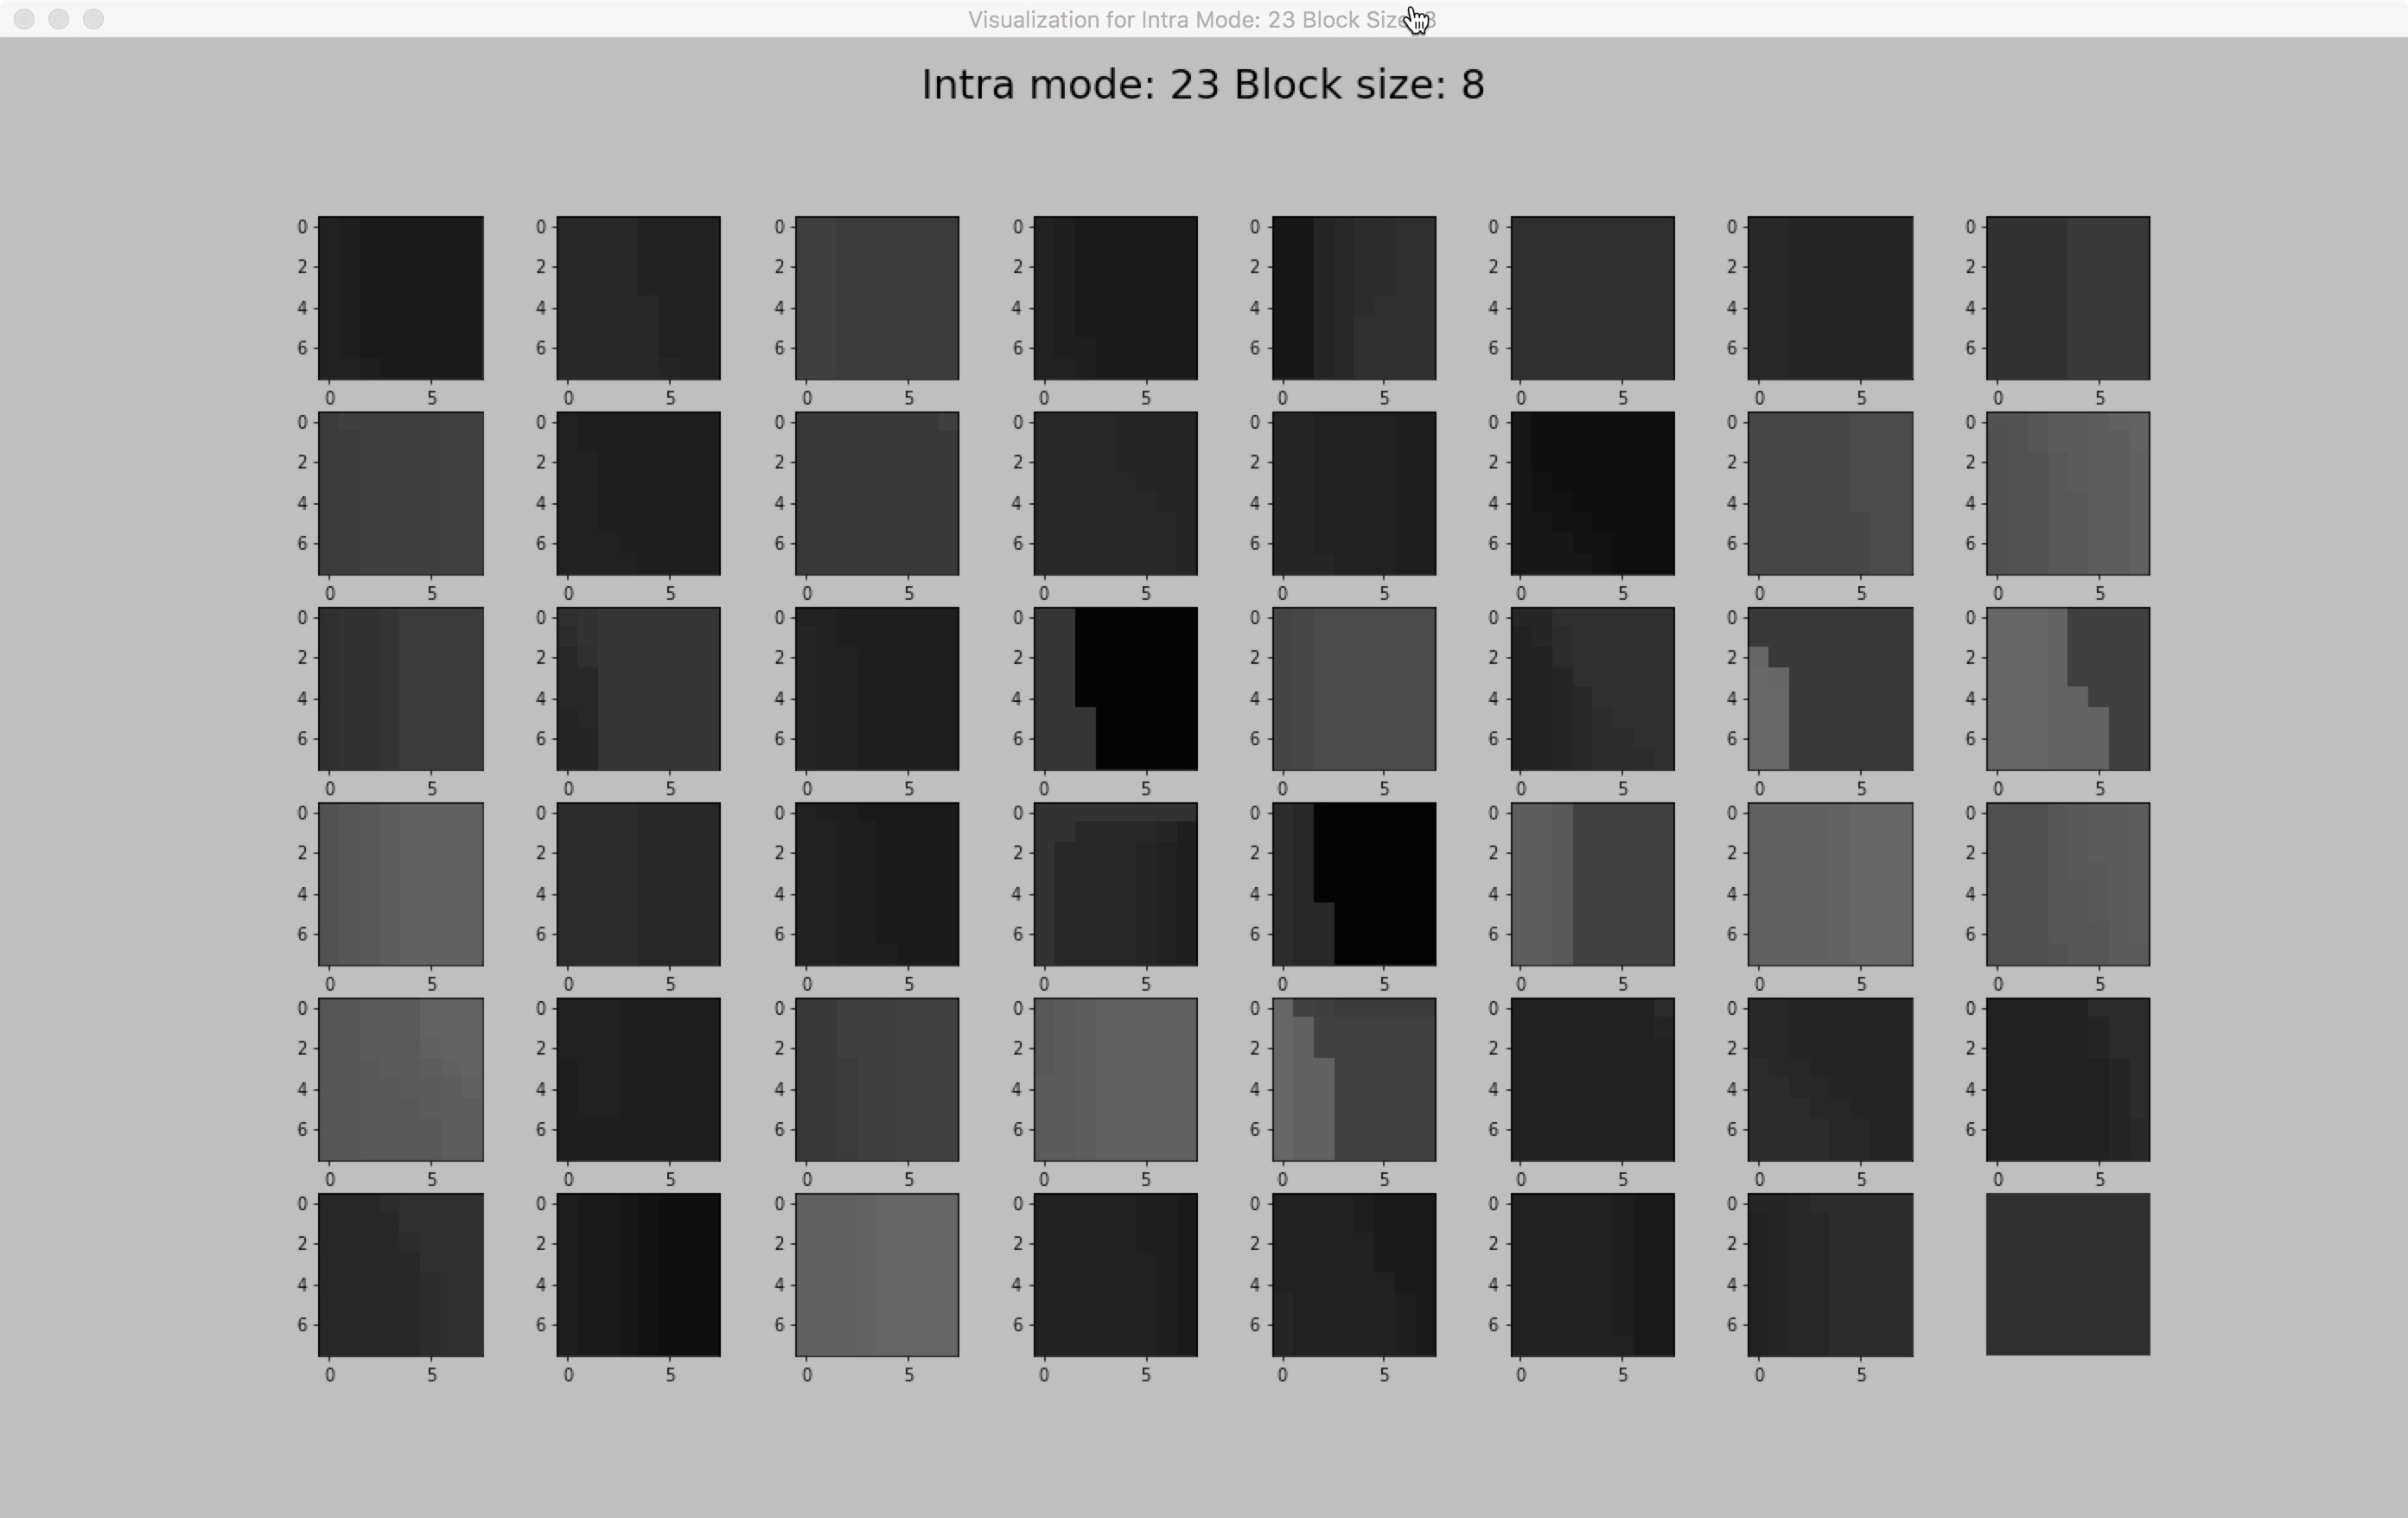
\includegraphics[width=\linewidth]{Figures/visu-size8x8/8-23}
        \caption[Intra mode 23]{intra mode 23.}
        \label{fig:size8_mode23}
    \end{minipage}

    \vspace*{1cm} % vertical separation

    \begin{minipage}{0.49\textwidth}
        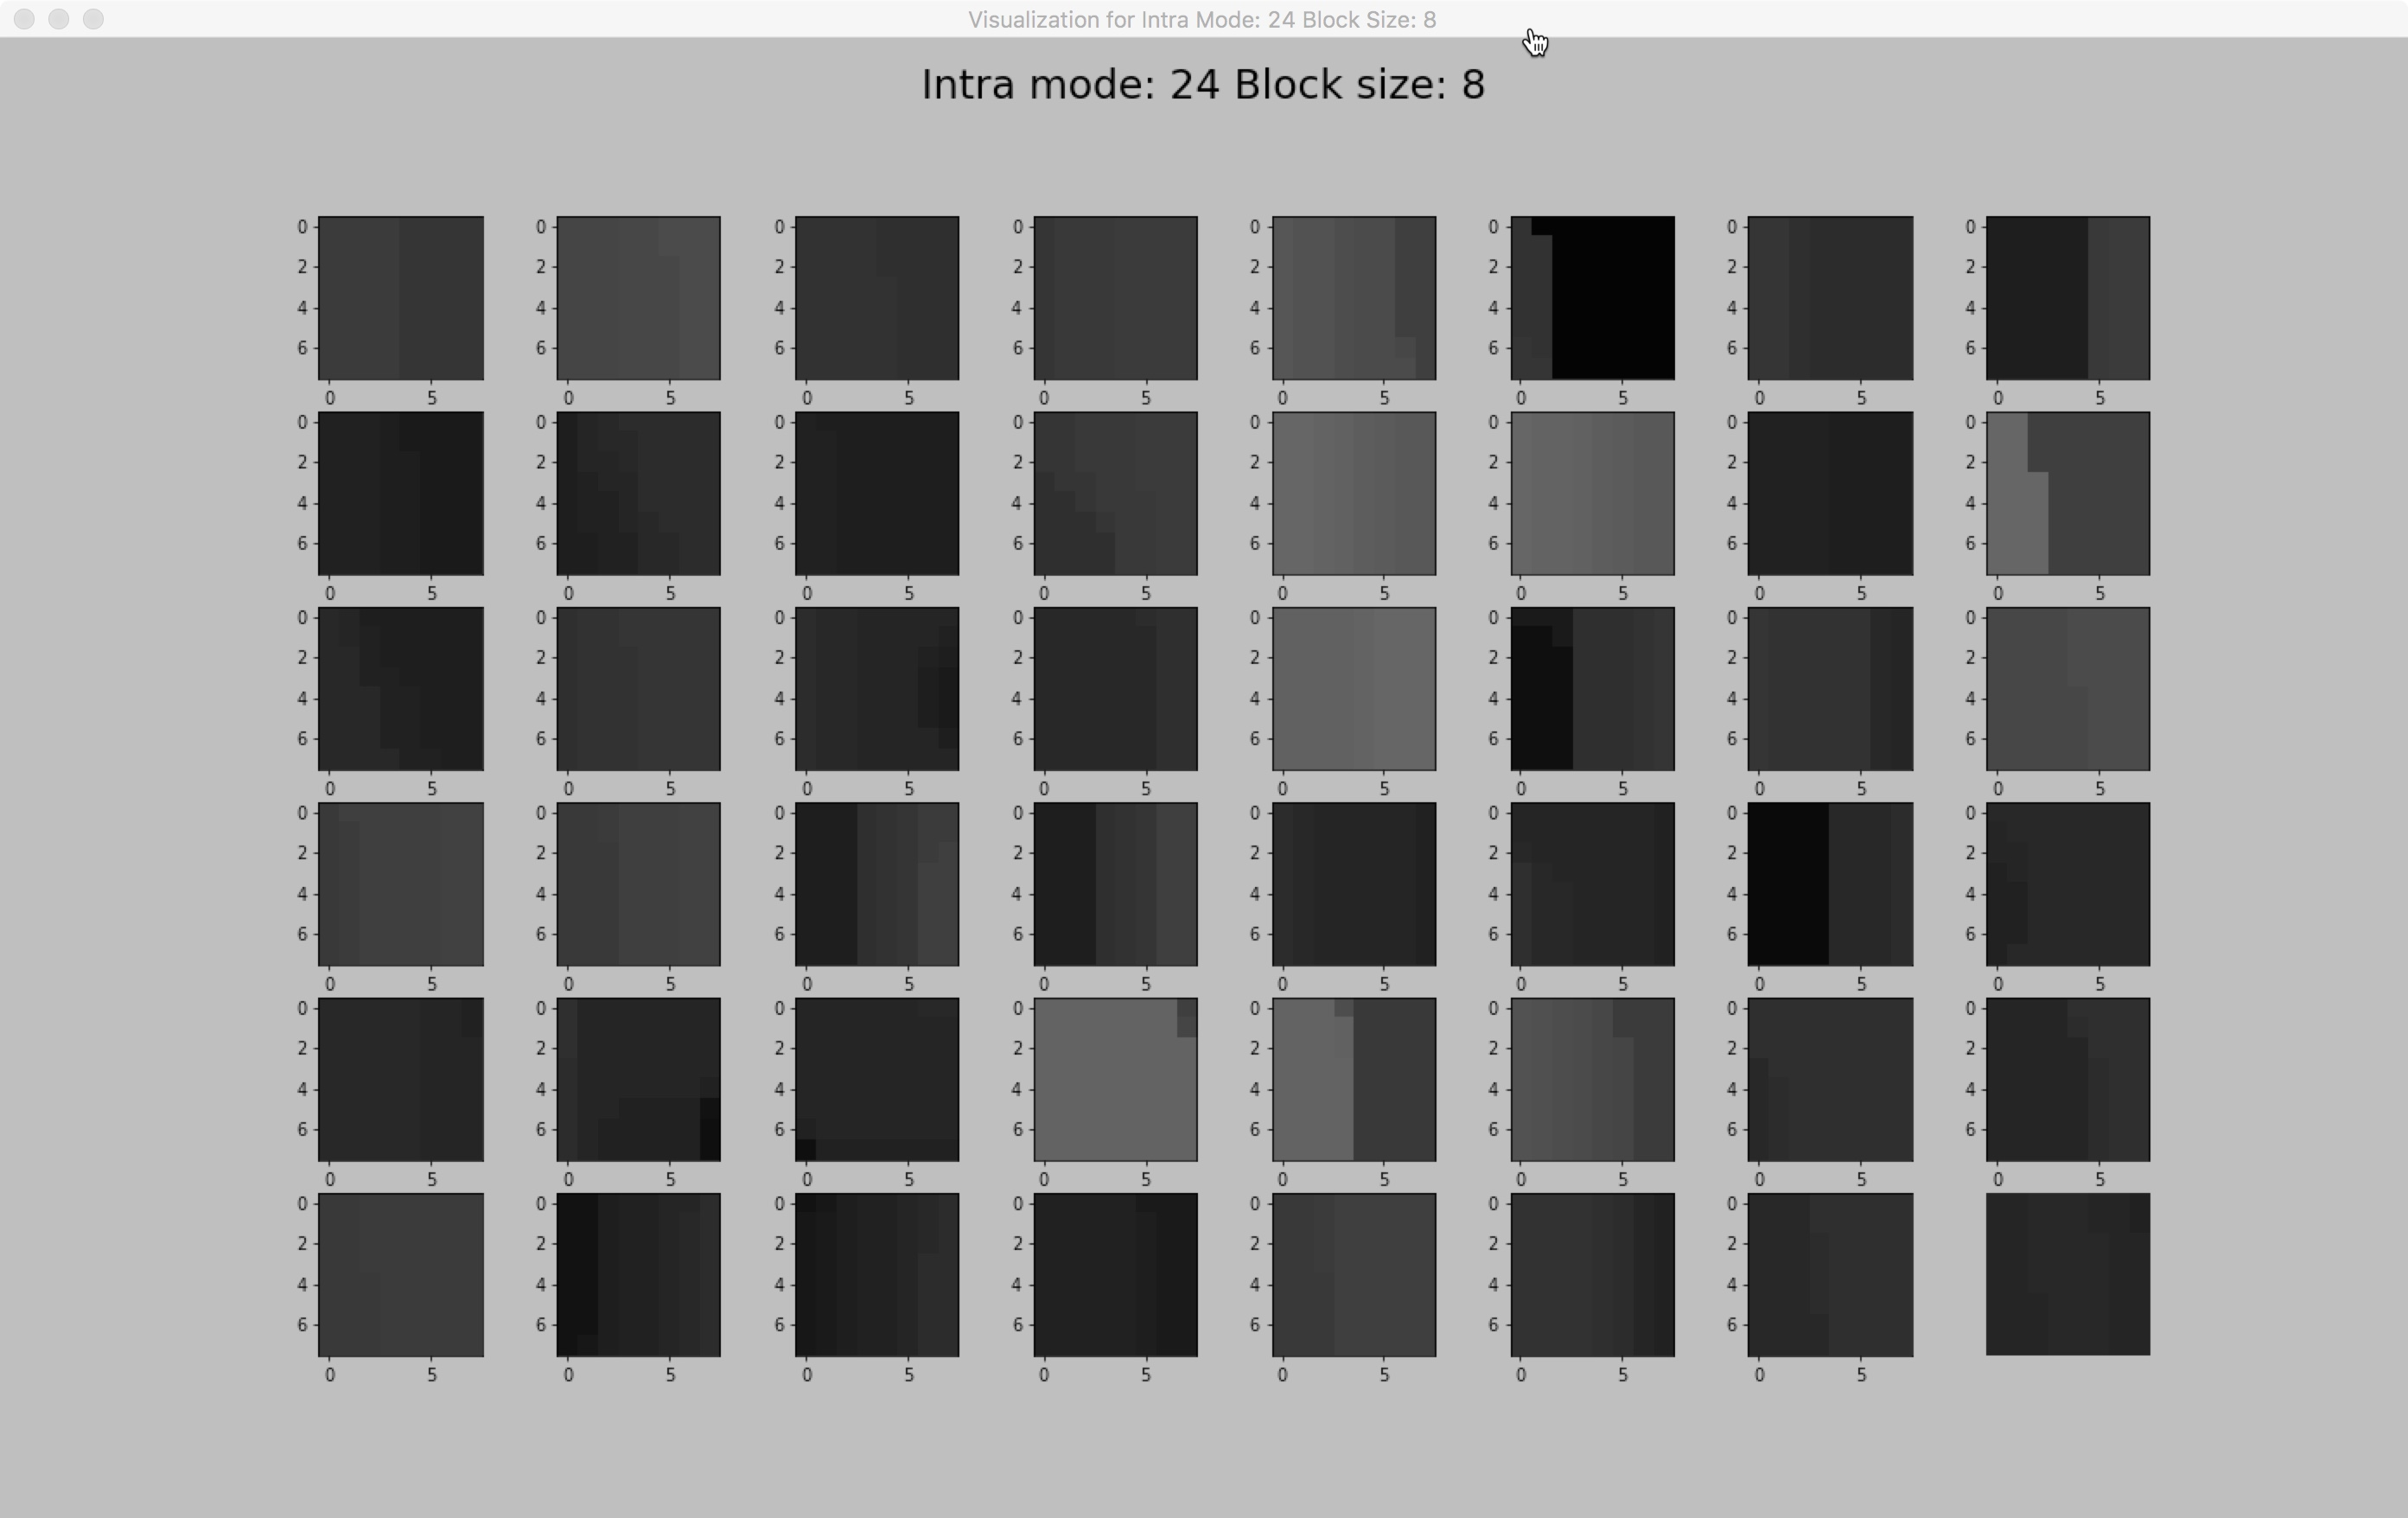
\includegraphics[width=\linewidth]{Figures/visu-size8x8/8-24}
        \caption[Intra mode 24]{intra mode 24.}
        \label{fig:size8_mode24}
    \end{minipage}
    \hspace{\fill} % note: no blank line here
    \begin{minipage}{0.49\textwidth}
        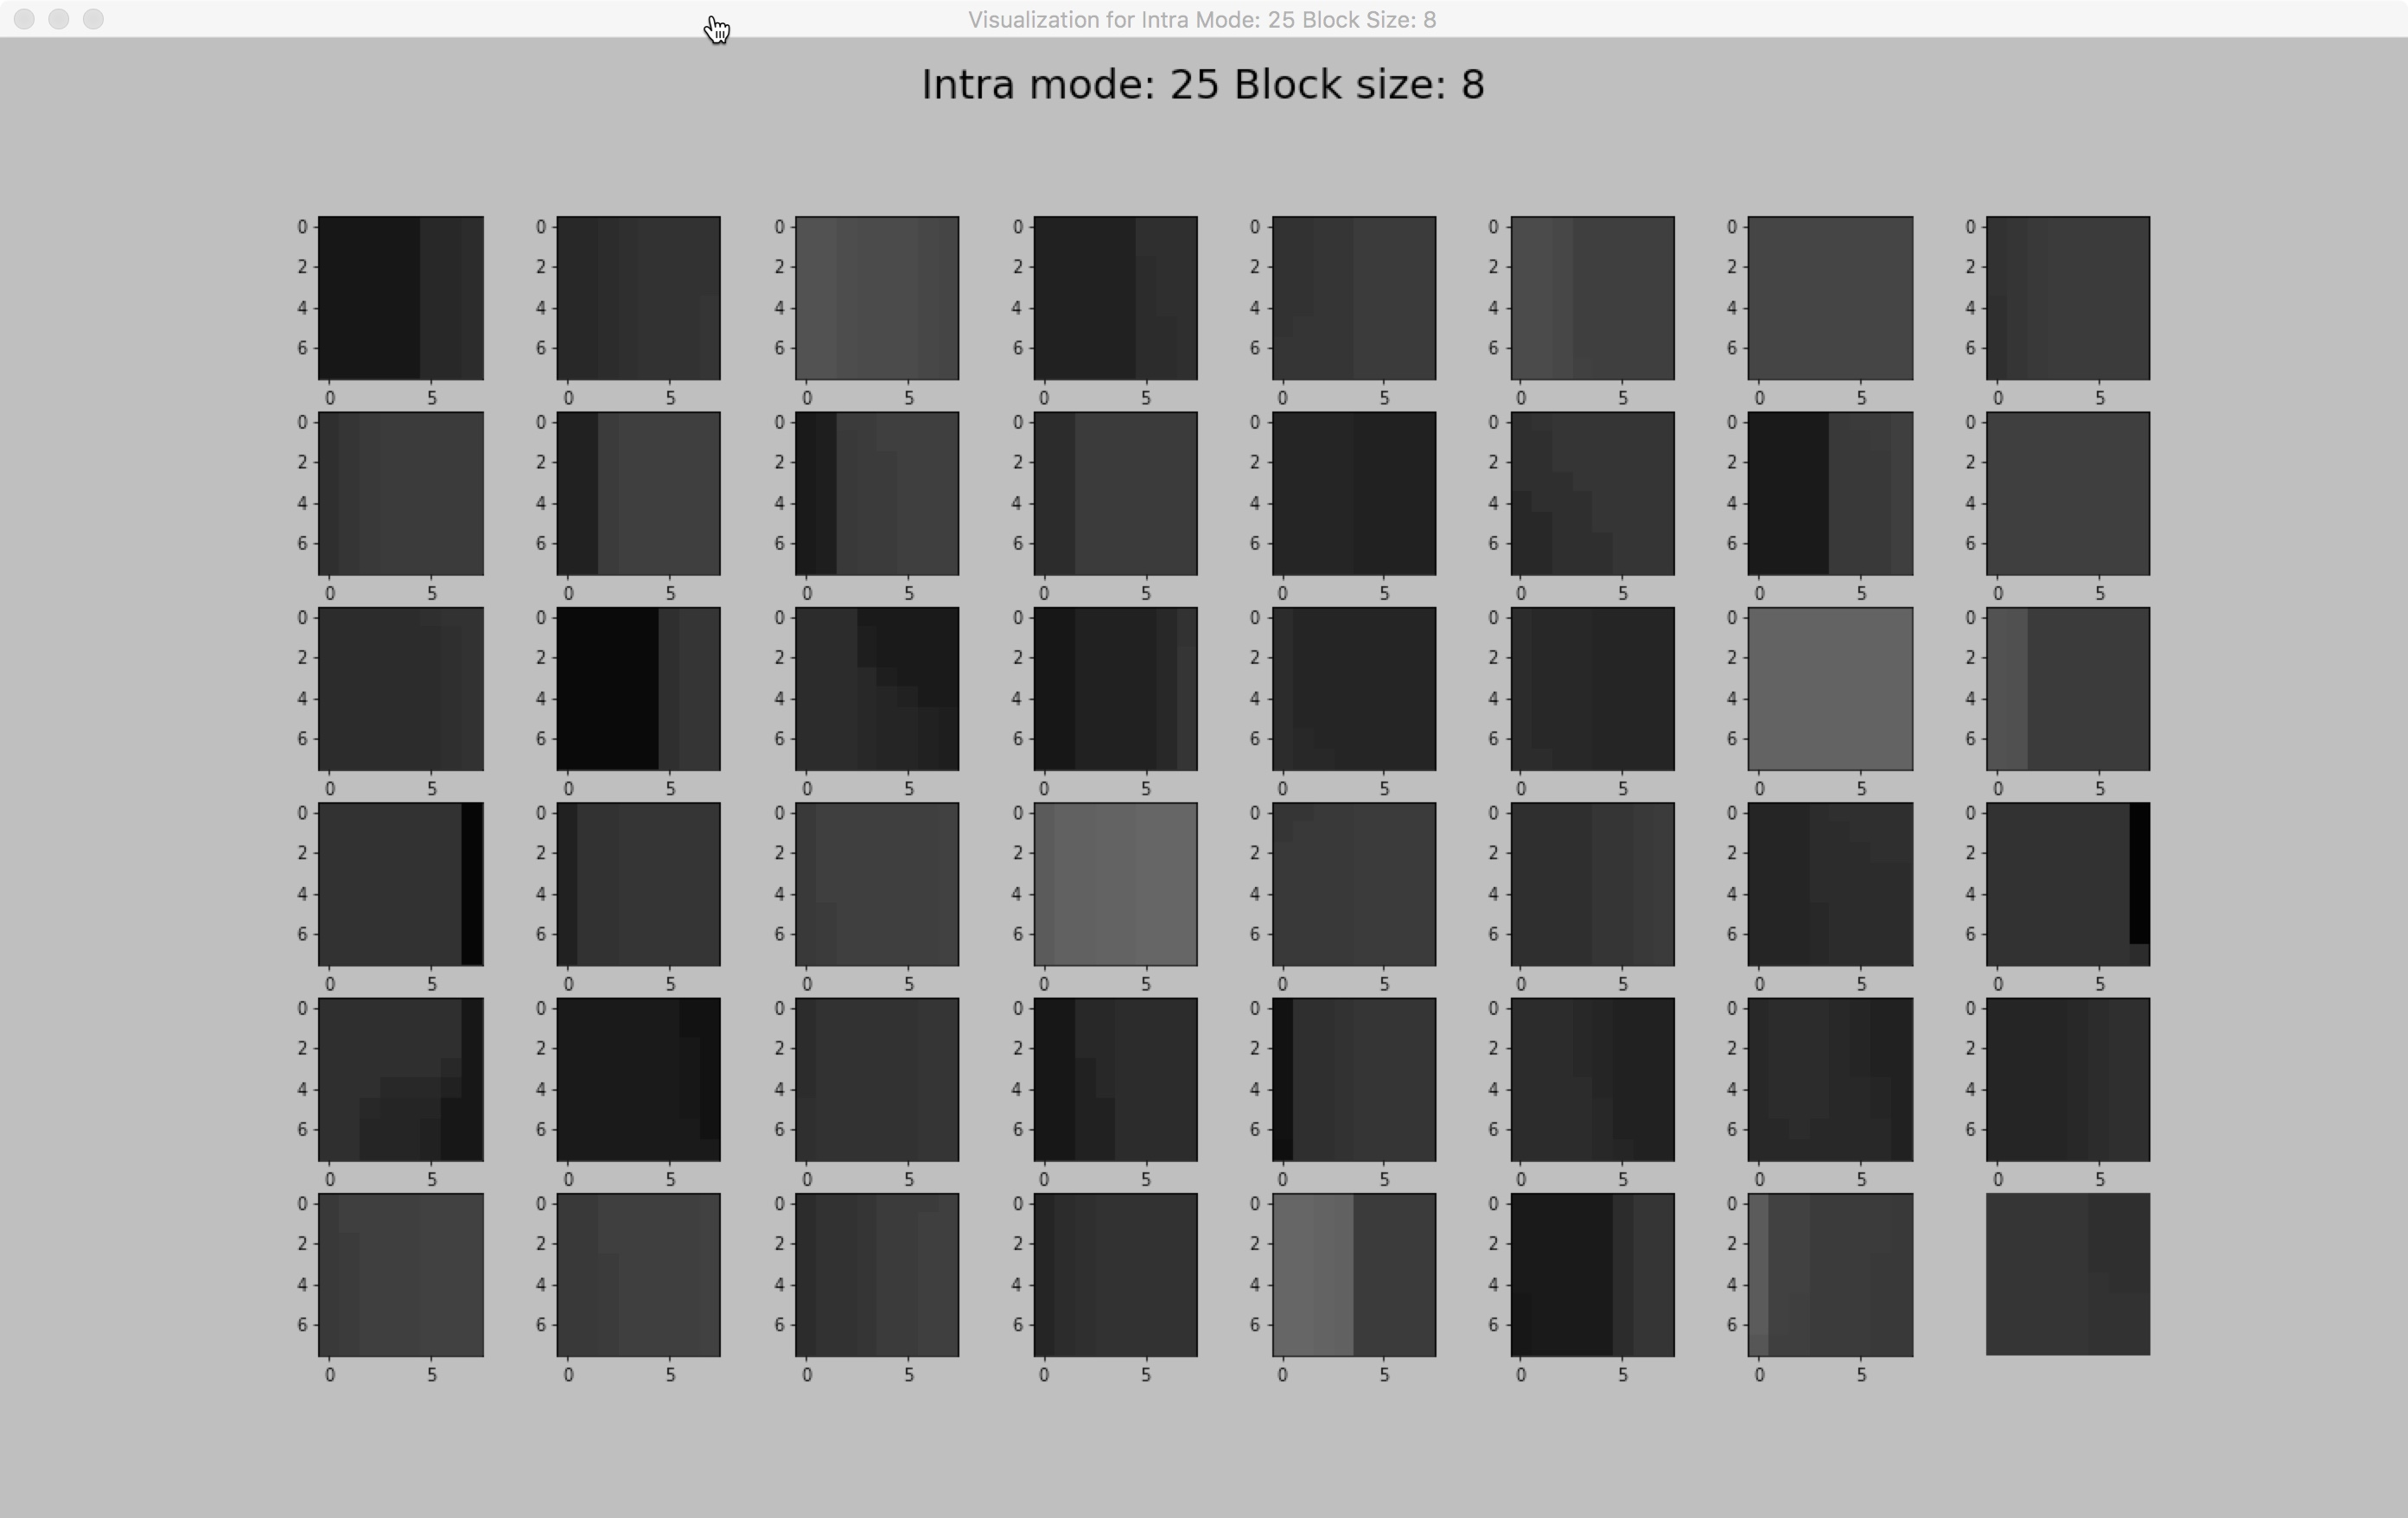
\includegraphics[width=\linewidth]{Figures/visu-size8x8/8-25}
        \caption[Intra mode 25]{intra mode 25.}
        \label{fig:size8_mode25}
    \end{minipage}
    
    \vspace*{1cm} % vertical separation

    \begin{minipage}{0.49\textwidth}
        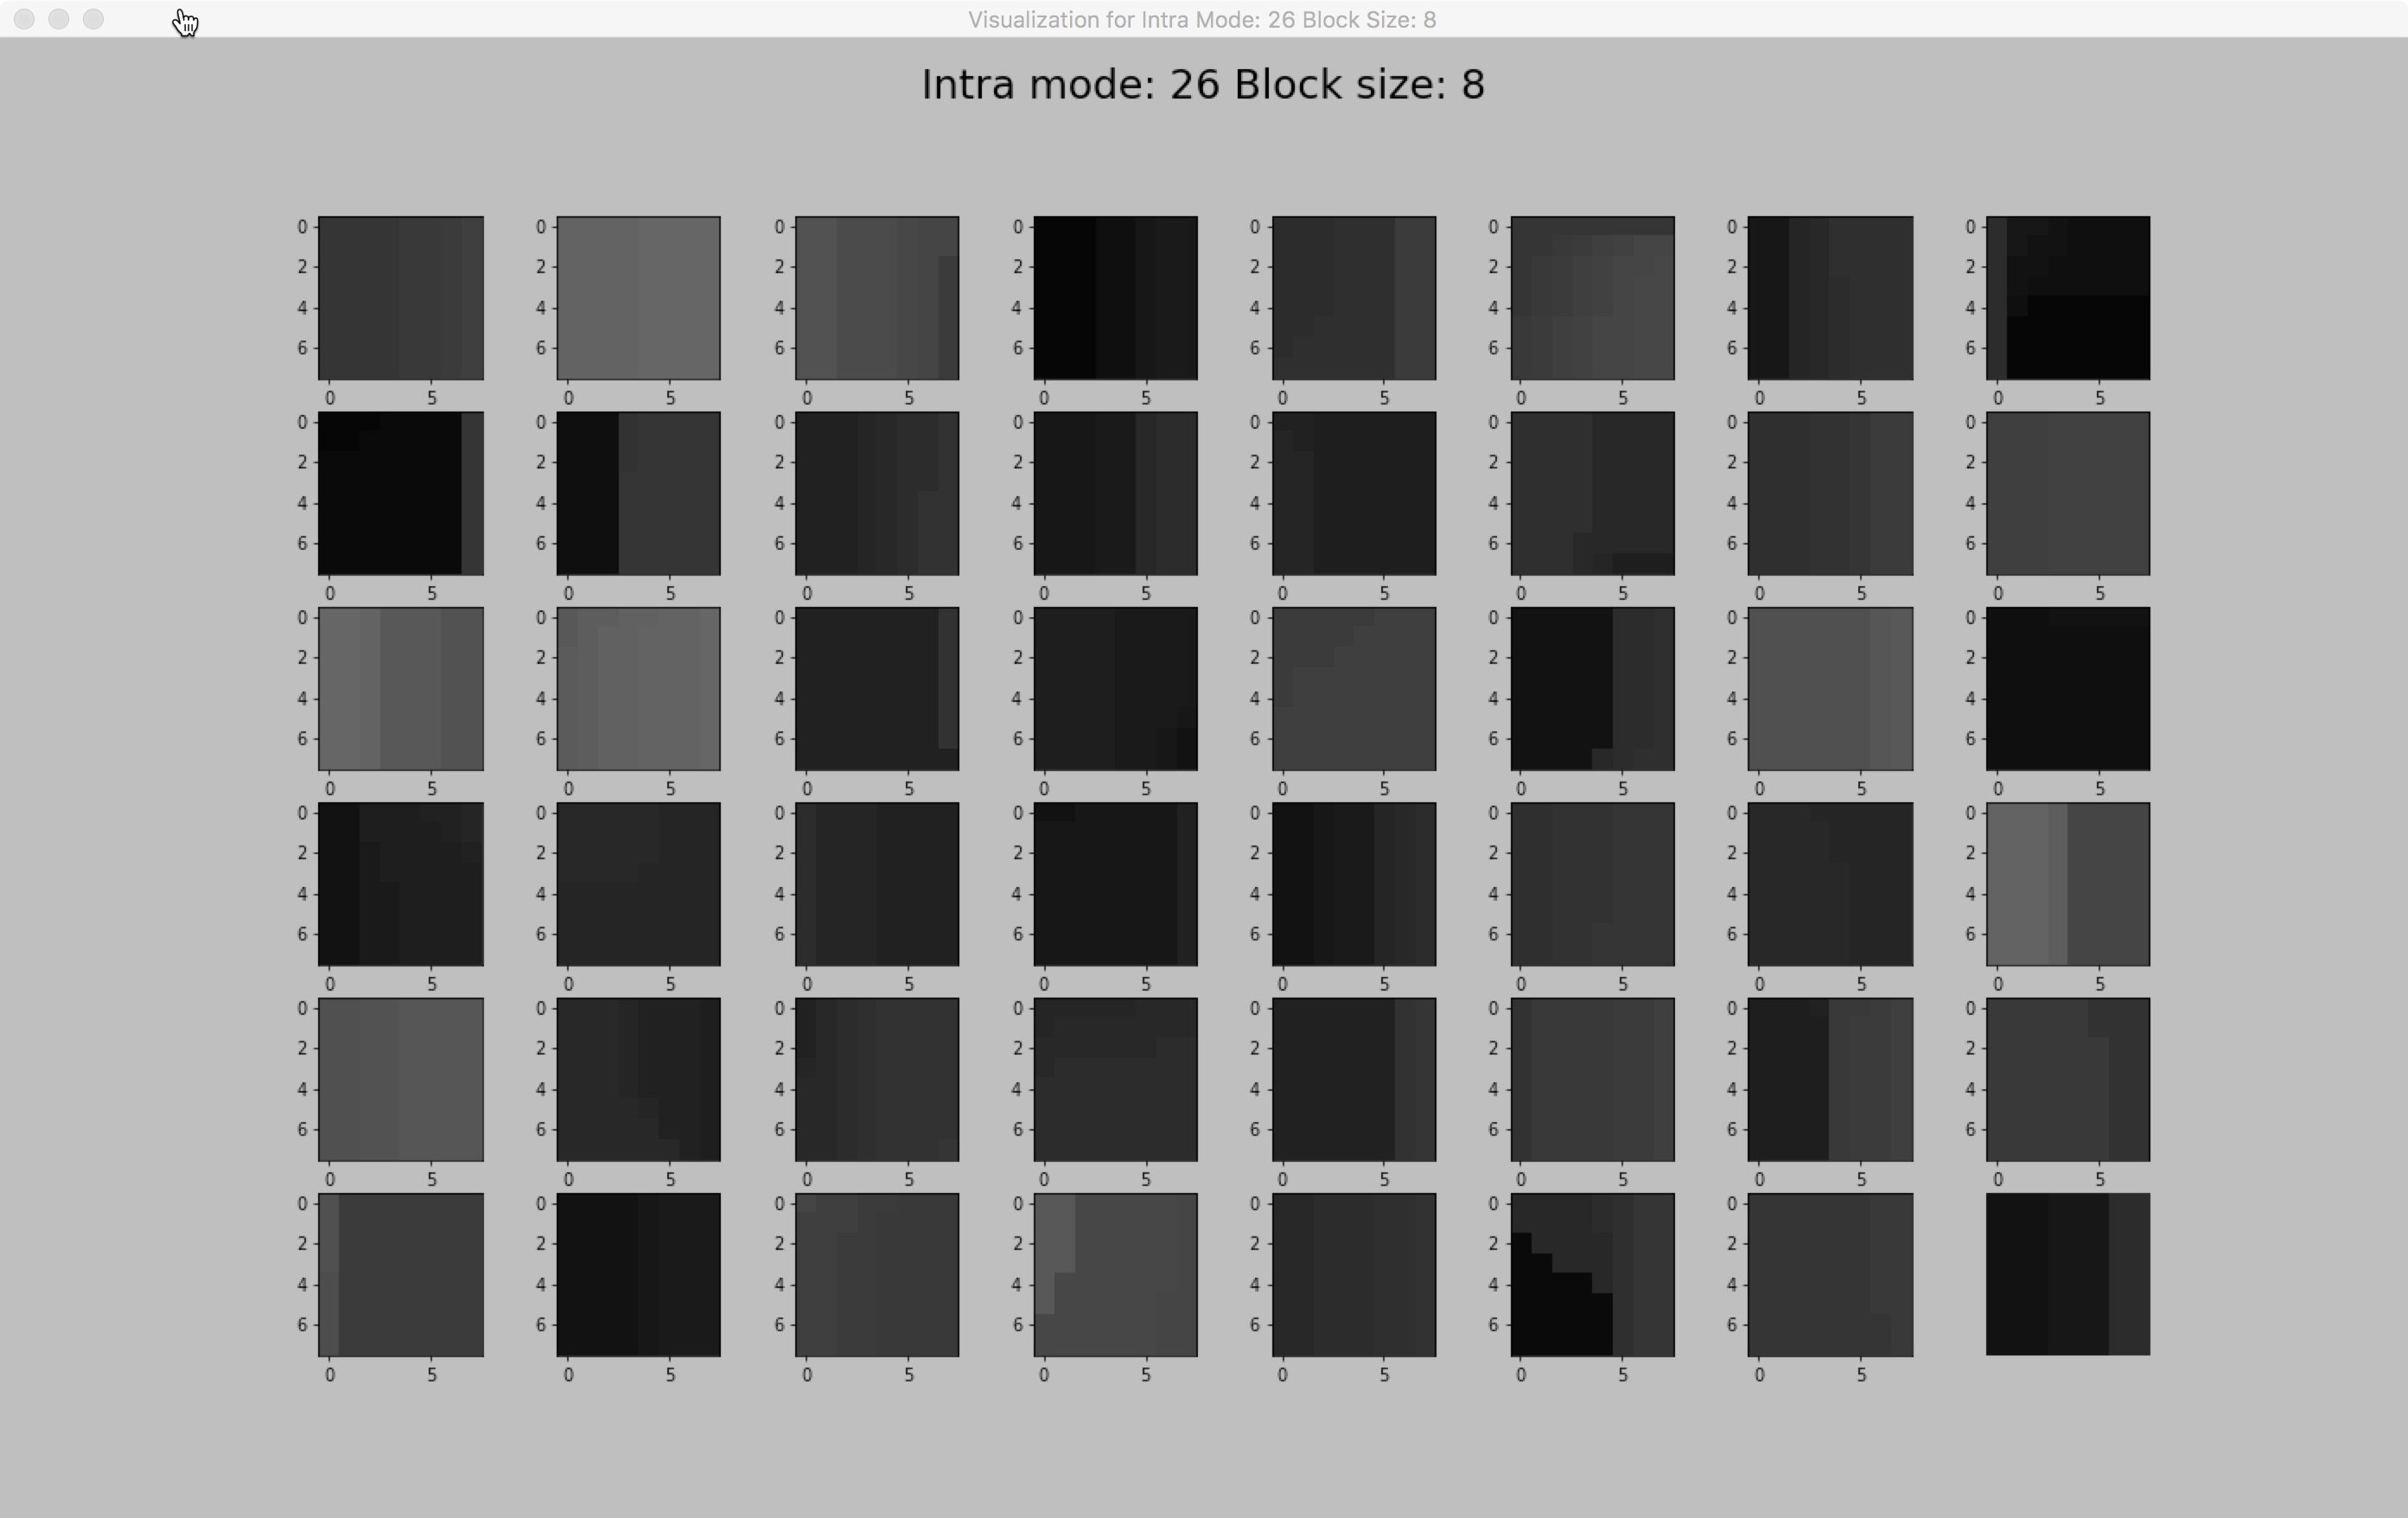
\includegraphics[width=\linewidth]{Figures/visu-size8x8/8-26}
        \caption[Intra mode 26]{intra mode 26.}
        \label{fig:size8_mode26}
    \end{minipage}
    \hspace{\fill} % note: no blank line here
    \begin{minipage}{0.49\textwidth}
        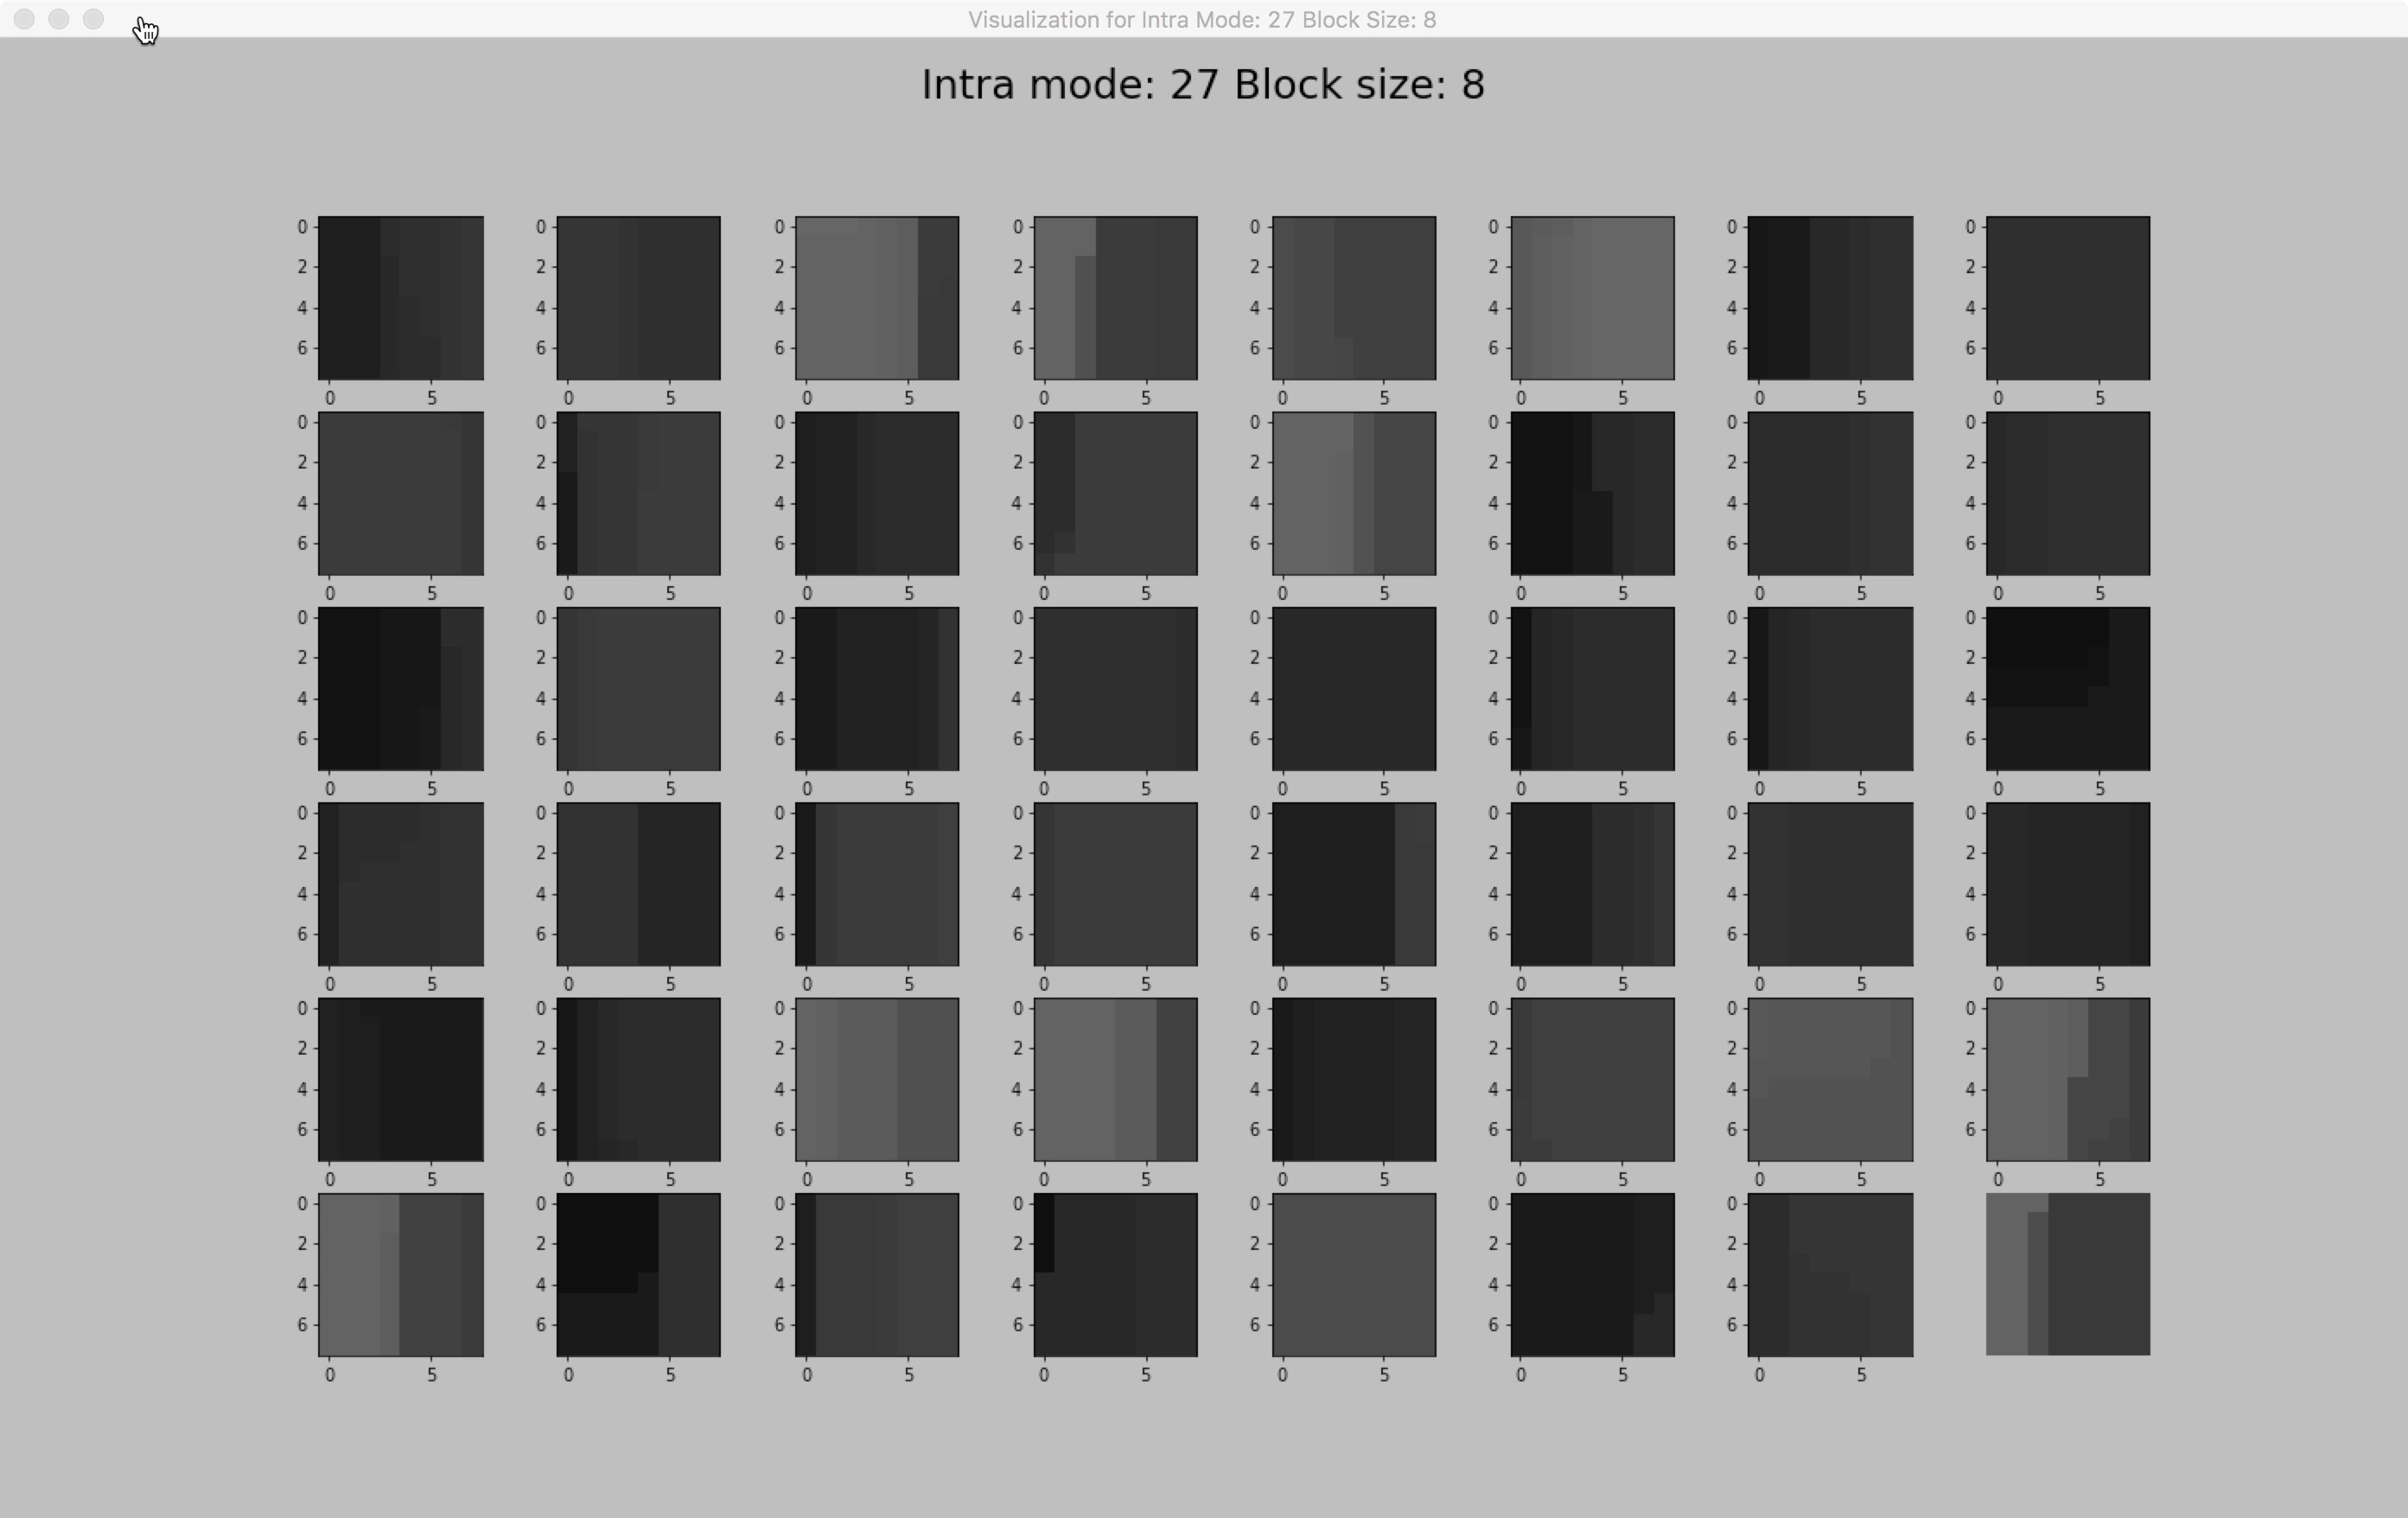
\includegraphics[width=\linewidth]{Figures/visu-size8x8/8-27}
        \caption[Intra mode 27]{intra mode 27.}
        \label{fig:size8_mode27}
    \end{minipage}
    % \caption{Figure caption goes here}\label{fig:visualizations-for-blocks-of-size8x8-01}
\end{figure}

\begin{figure}[H]

    \vspace*{1cm} % vertical separation

    \begin{minipage}{0.49\textwidth}
        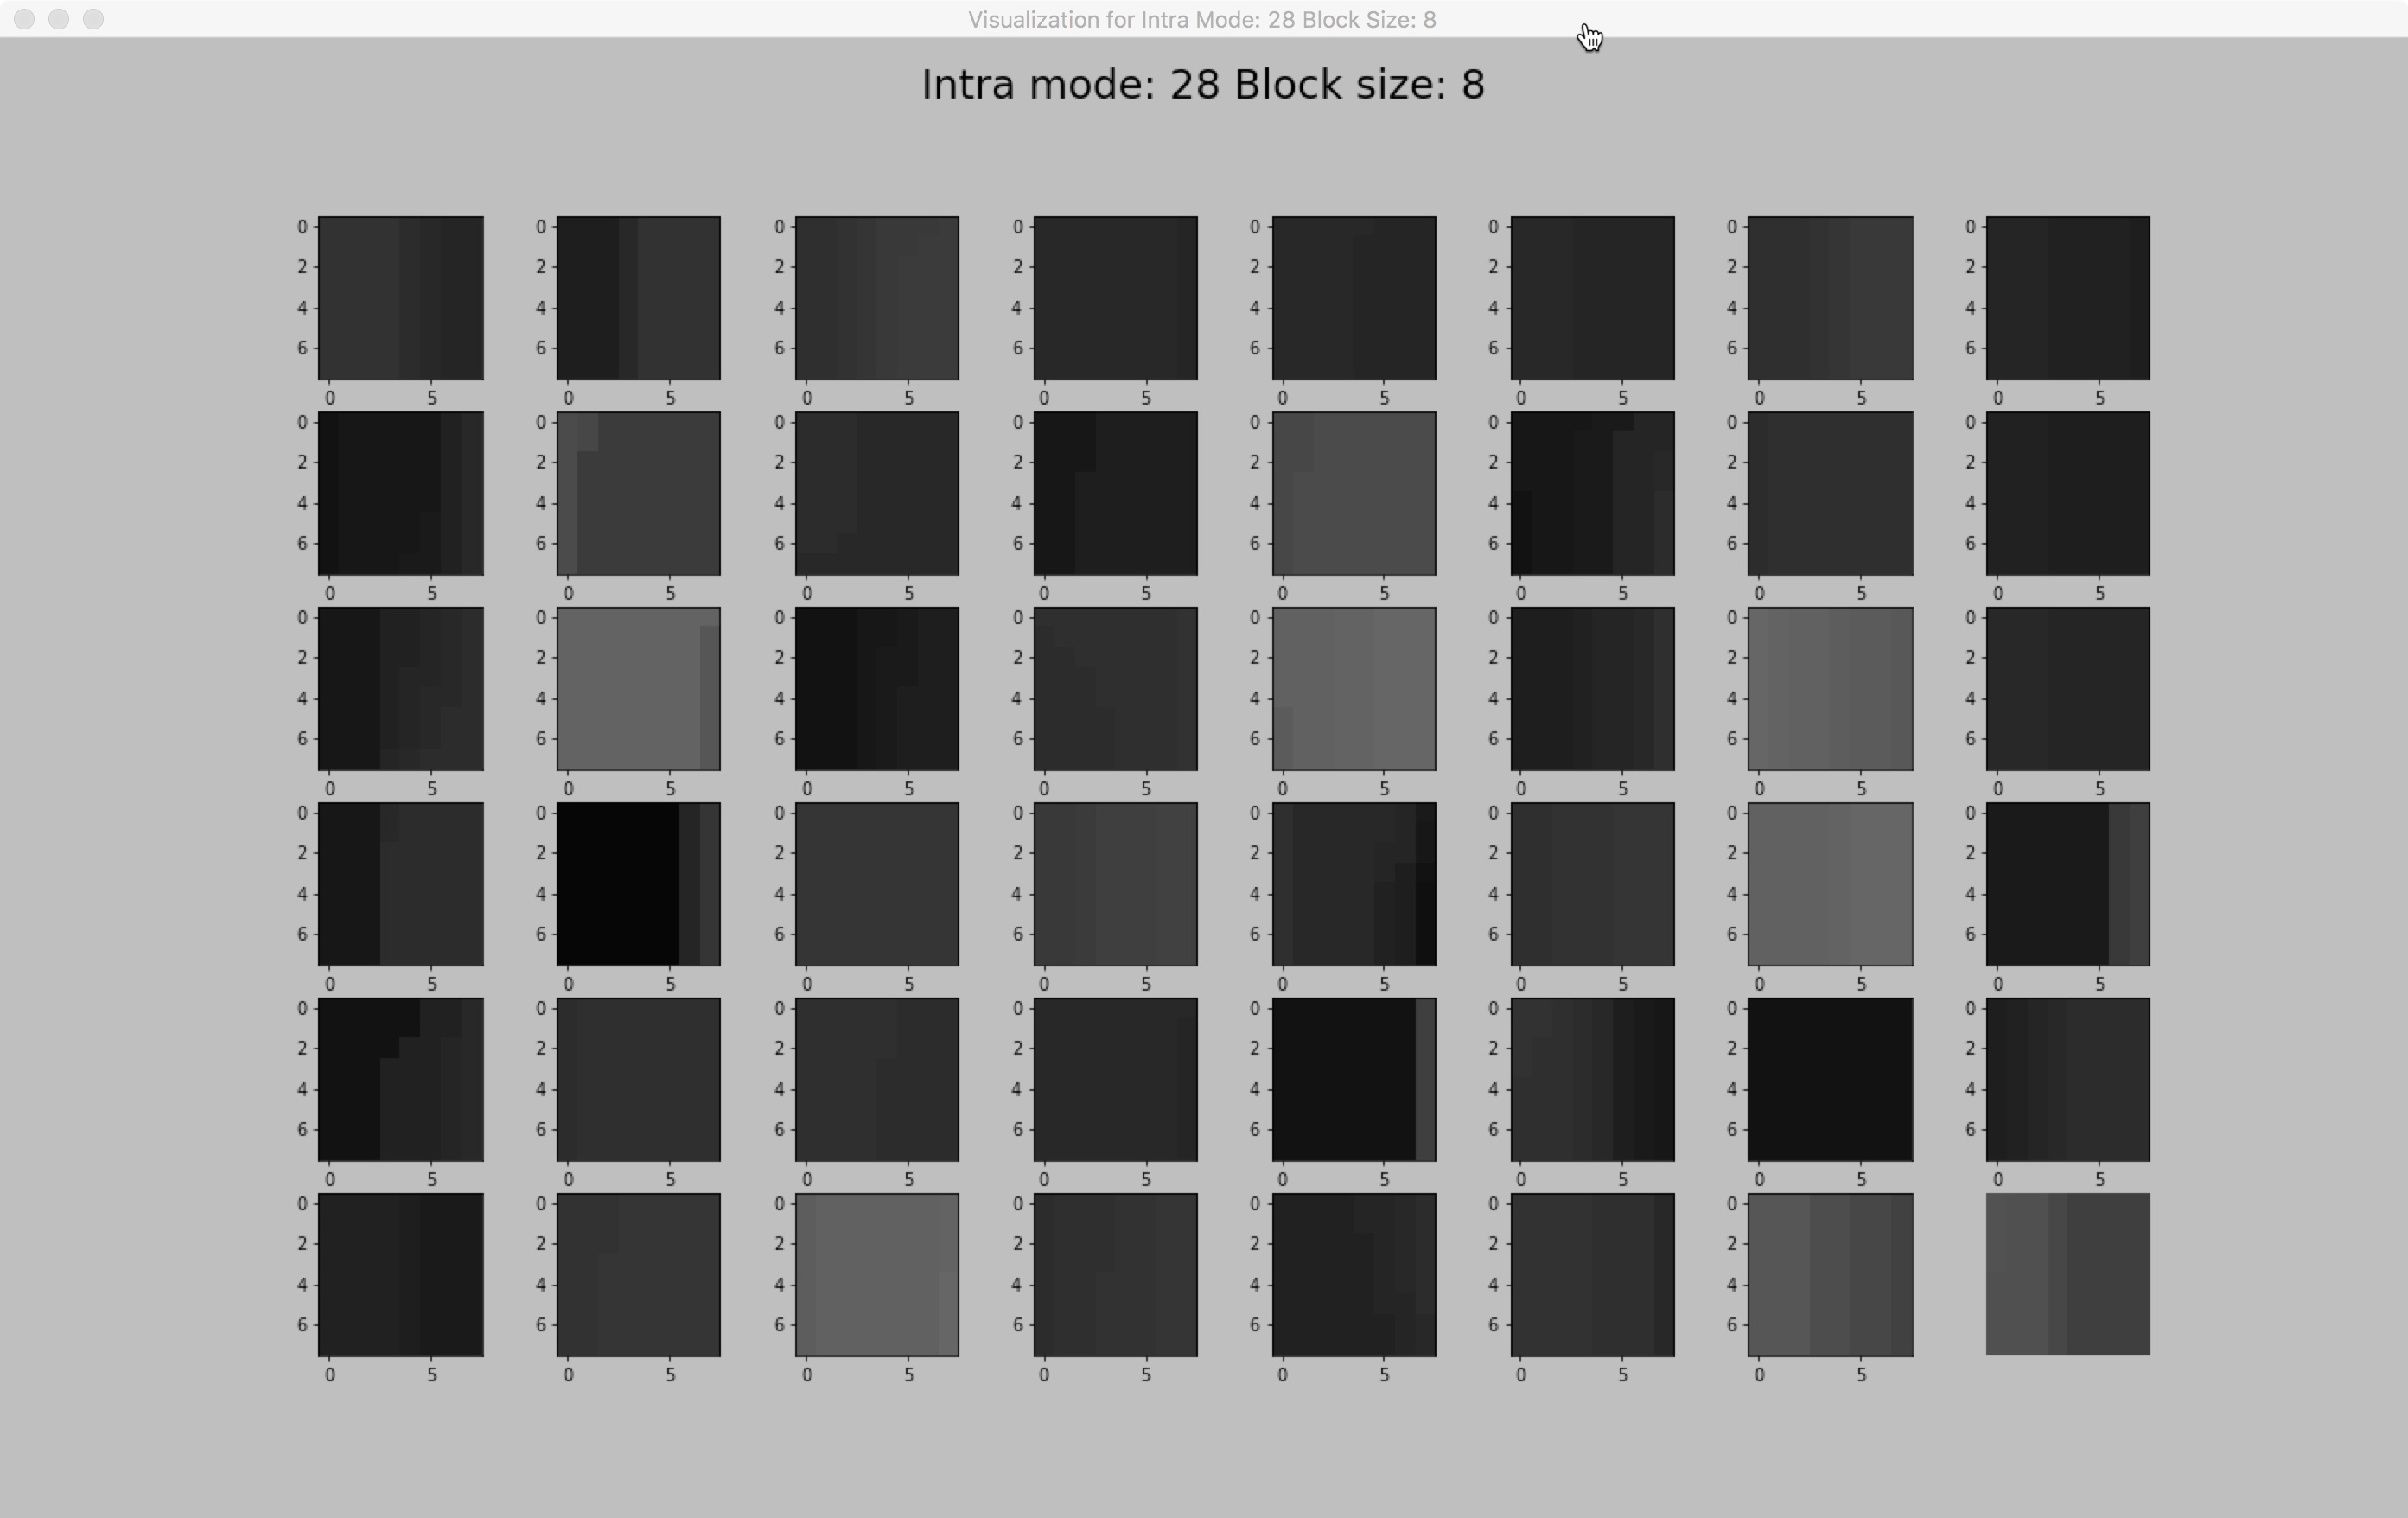
\includegraphics[width=\linewidth]{Figures/visu-size8x8/8-28}
        \caption[Intra mode 28]{intra mode 28.}
        \label{fig:size8_mode28}
    \end{minipage}
    \hspace{\fill} % note: no blank line here
    \begin{minipage}{0.49\textwidth}
        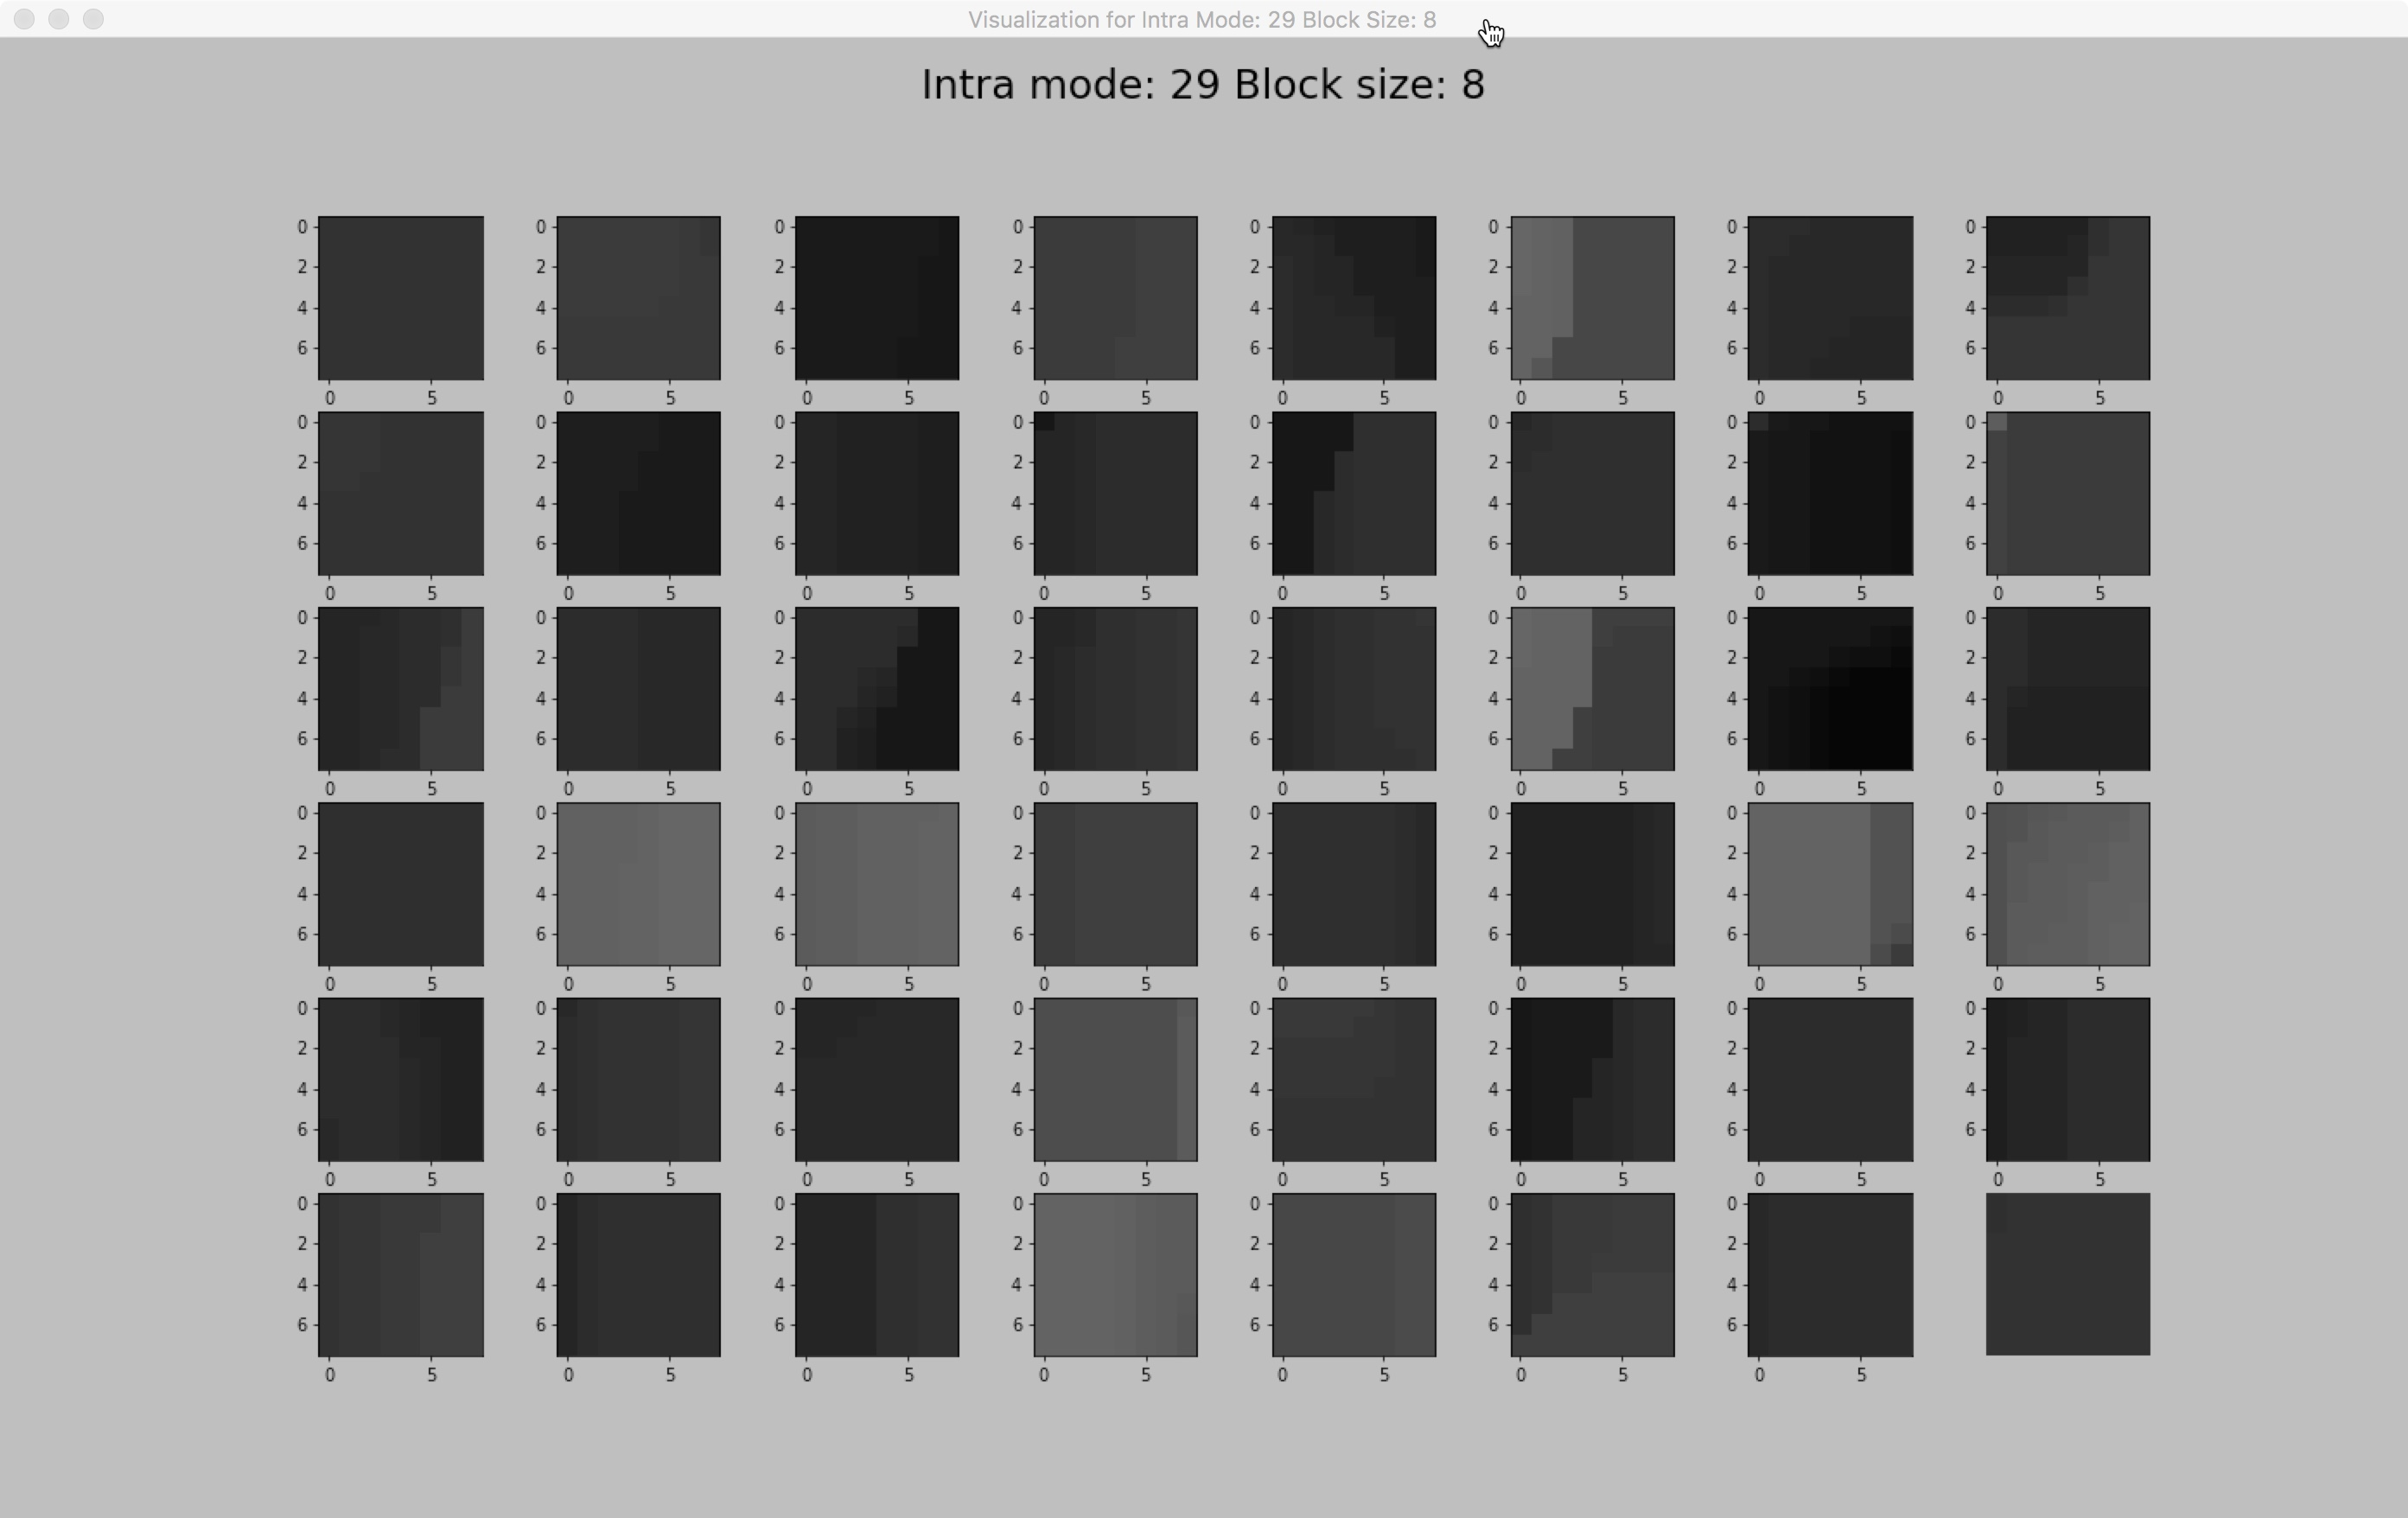
\includegraphics[width=\linewidth]{Figures/visu-size8x8/8-29}
        \caption[Intra mode 29]{intra mode 29.}
        \label{fig:size8_mode29}
    \end{minipage}

    \vspace*{1cm} % vertical separation

    \begin{minipage}{0.49\textwidth}
        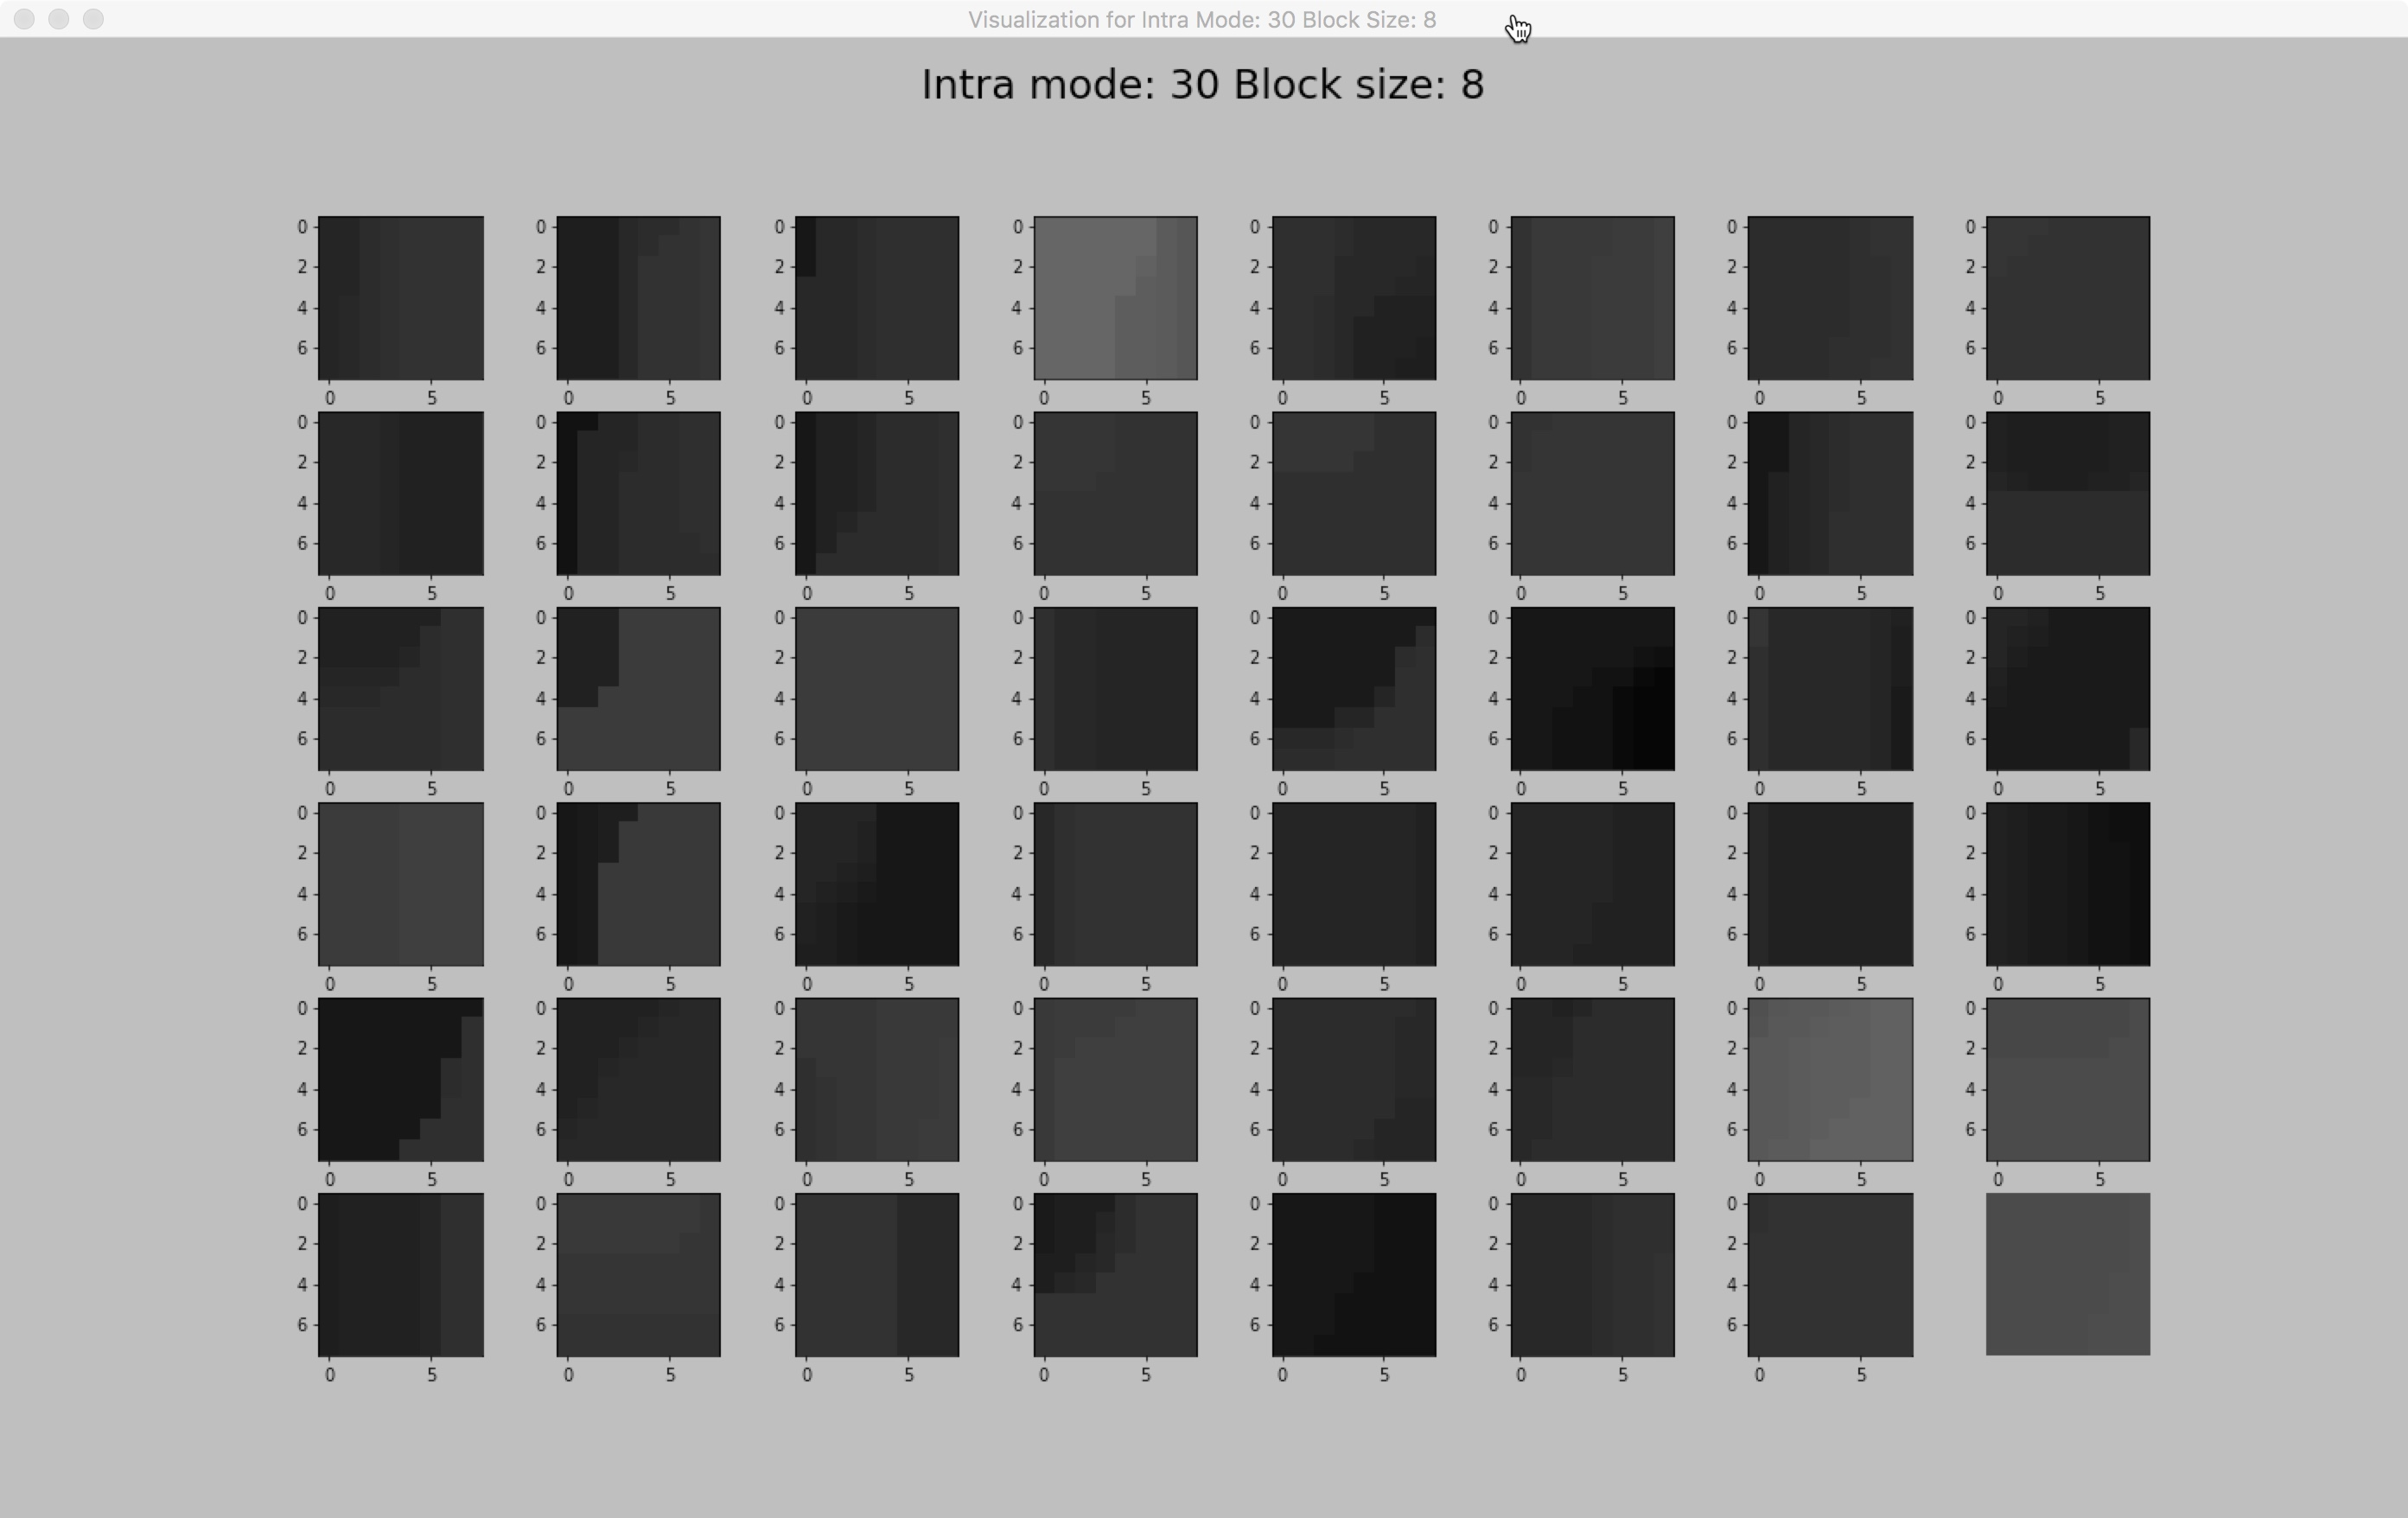
\includegraphics[width=\linewidth]{Figures/visu-size8x8/8-30}
        \caption[Intra mode 30]{intra mode 30.}
        \label{fig:size8_mode30}
    \end{minipage}
    \hspace{\fill} % note: no blank line here
    \begin{minipage}{0.49\textwidth}
        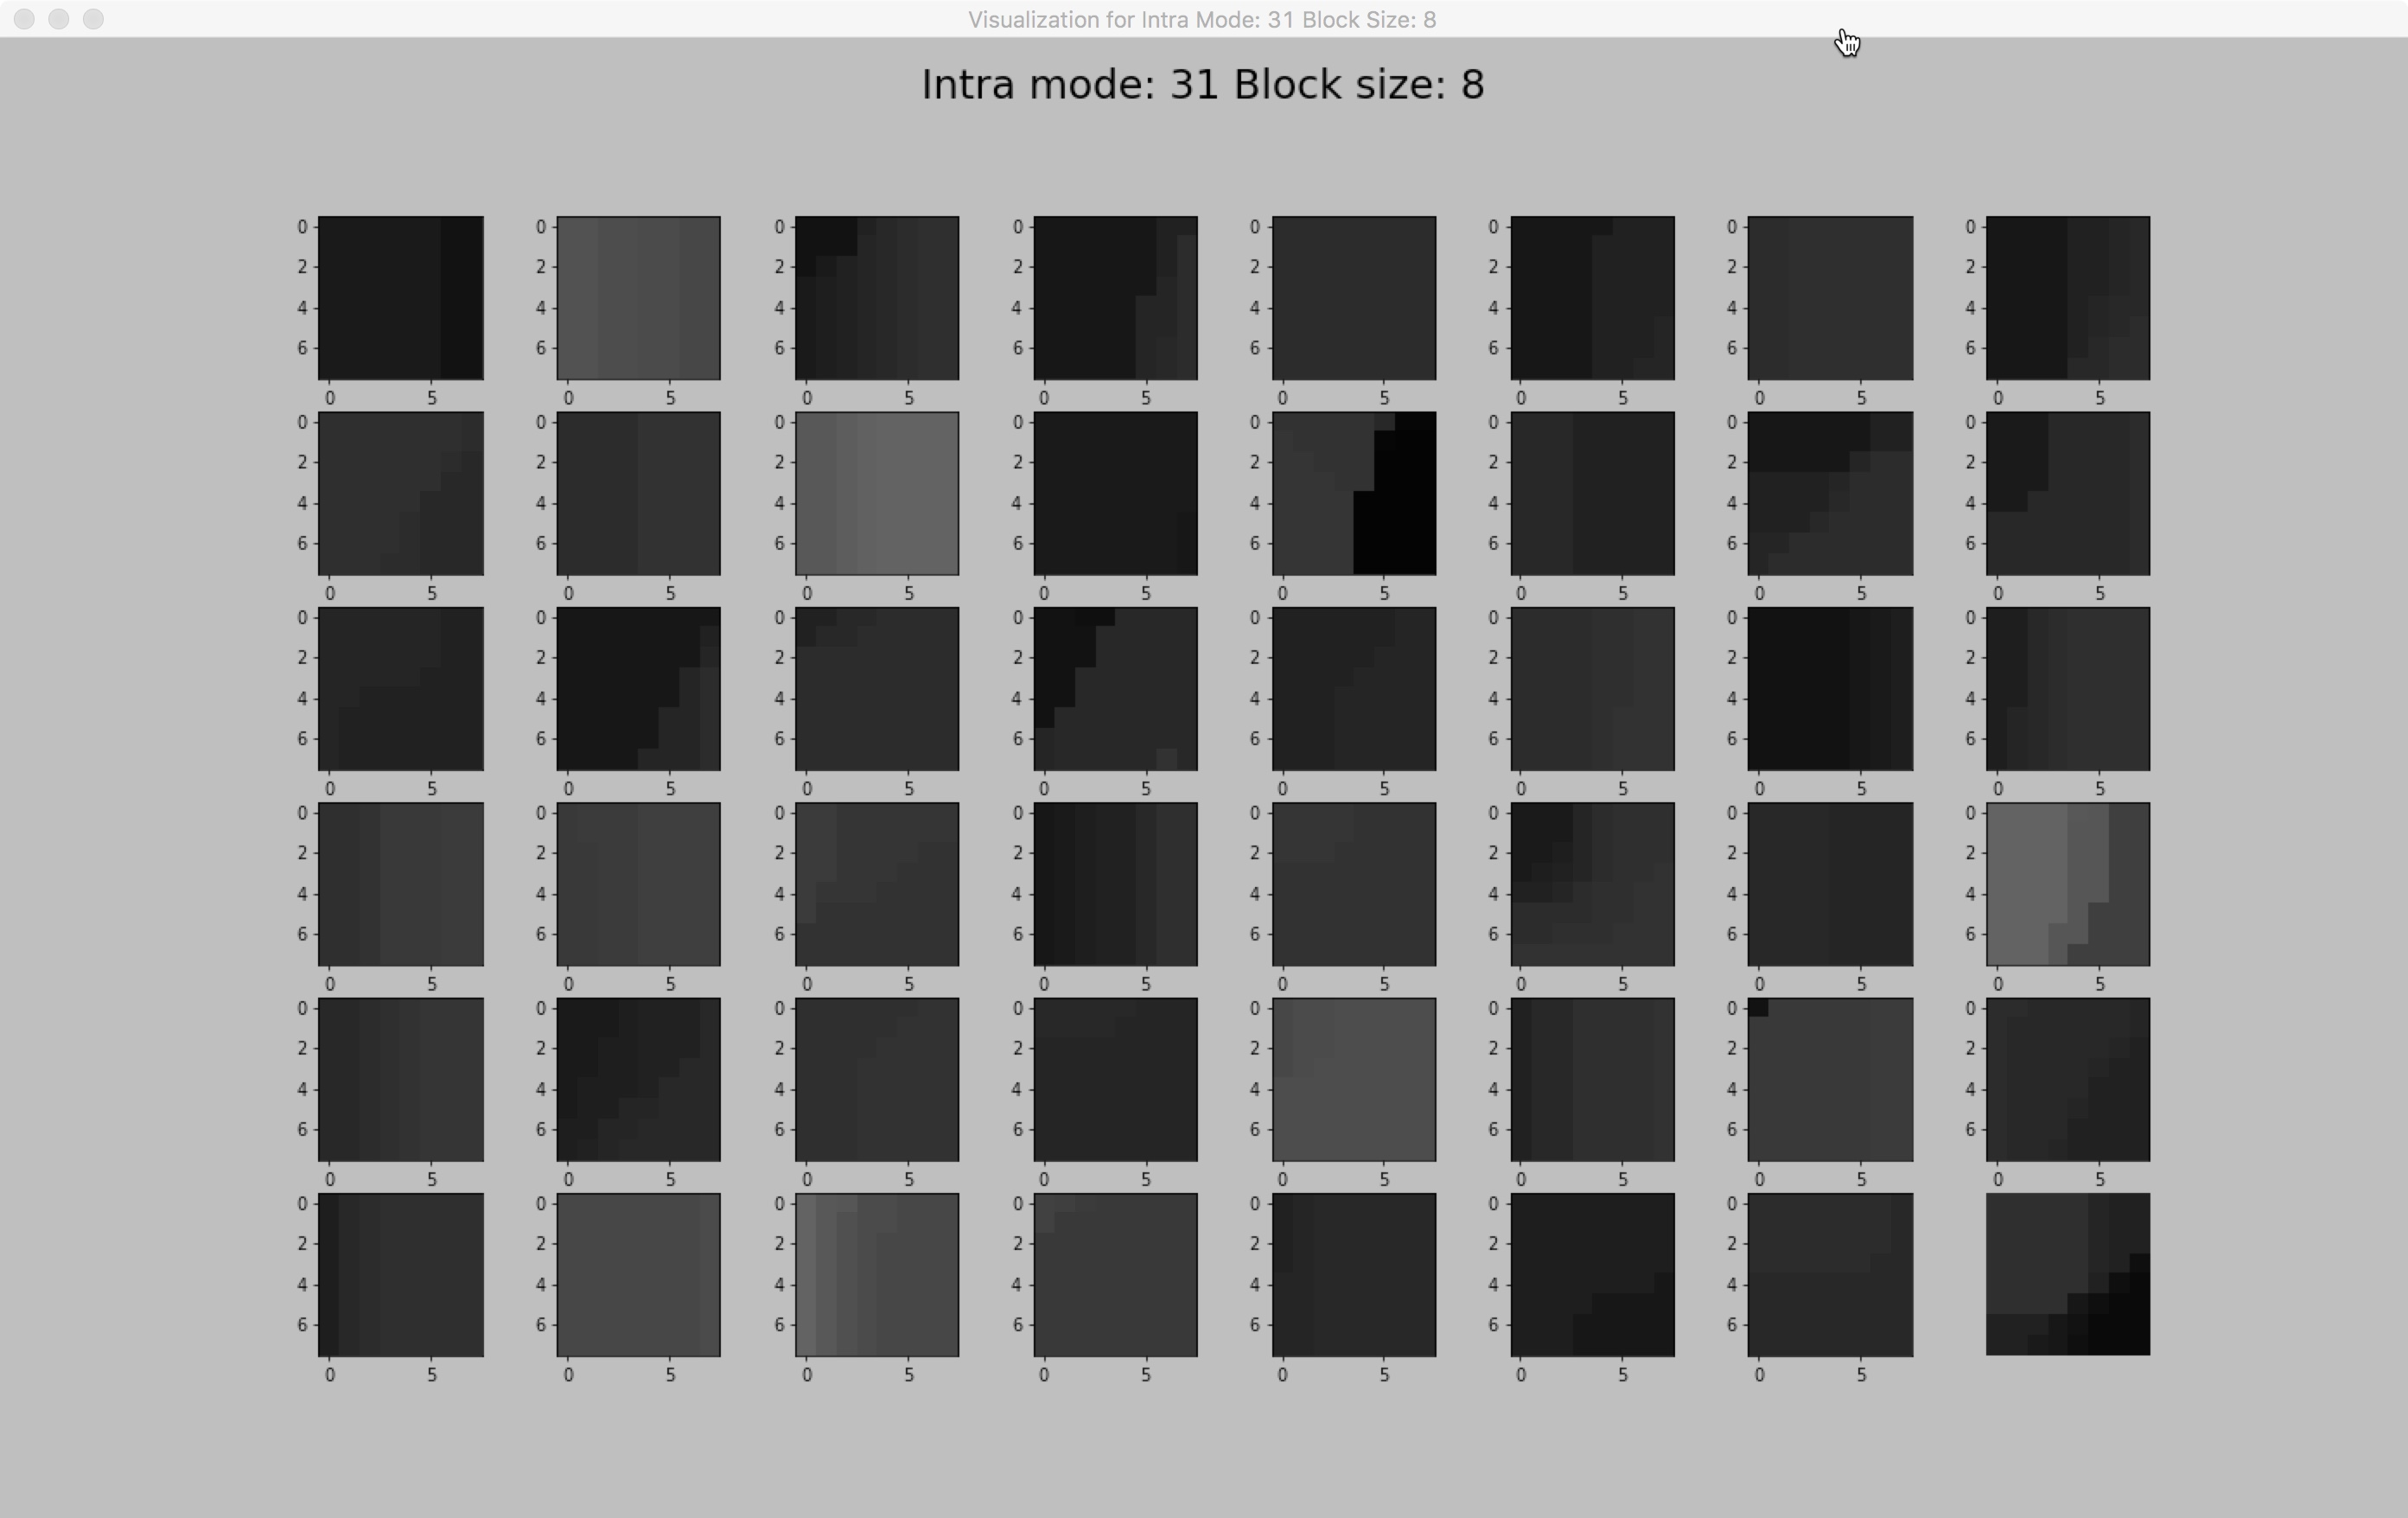
\includegraphics[width=\linewidth]{Figures/visu-size8x8/8-31}
        \caption[Intra mode 31]{intra mode 31.}
        \label{fig:size8_mode31}
    \end{minipage}
    
    \vspace*{1cm} % vertical separation

    \begin{minipage}{0.49\textwidth}
        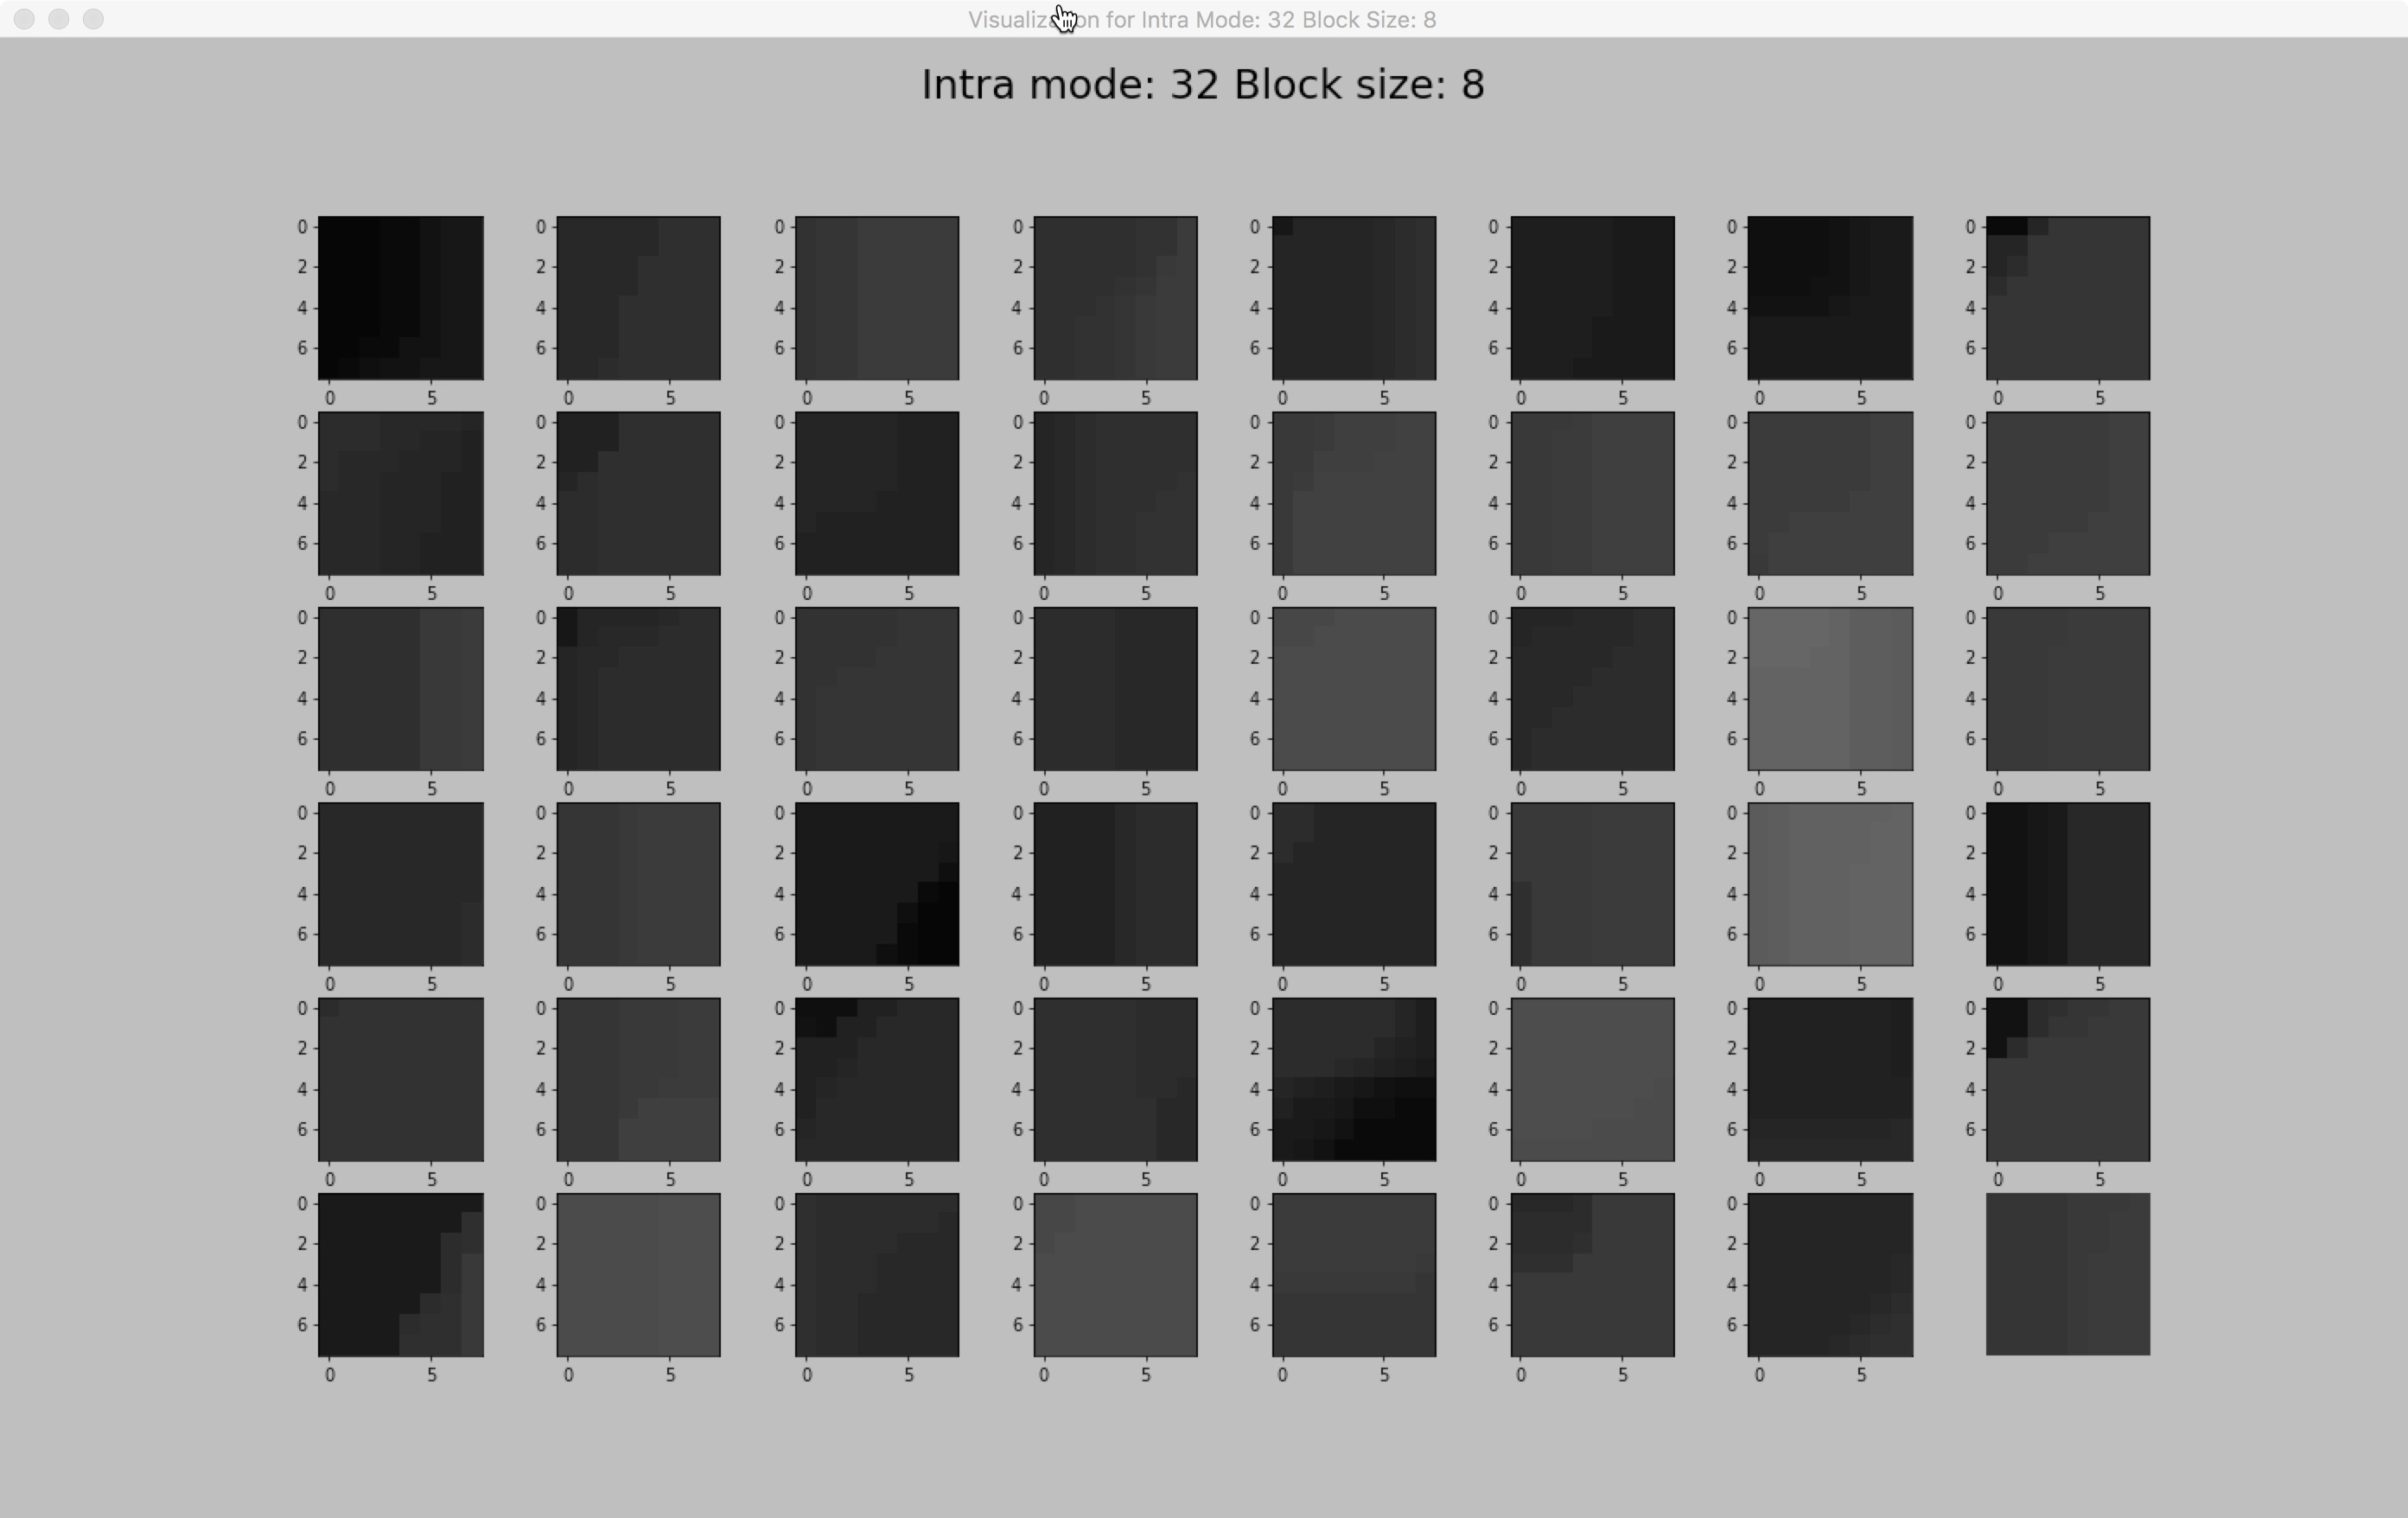
\includegraphics[width=\linewidth]{Figures/visu-size8x8/8-32}
        \caption[Intra mode 32]{intra mode 32.}
        \label{fig:size8_mode32}
    \end{minipage}
    \hspace{\fill} % note: no blank line here
    \begin{minipage}{0.49\textwidth}
        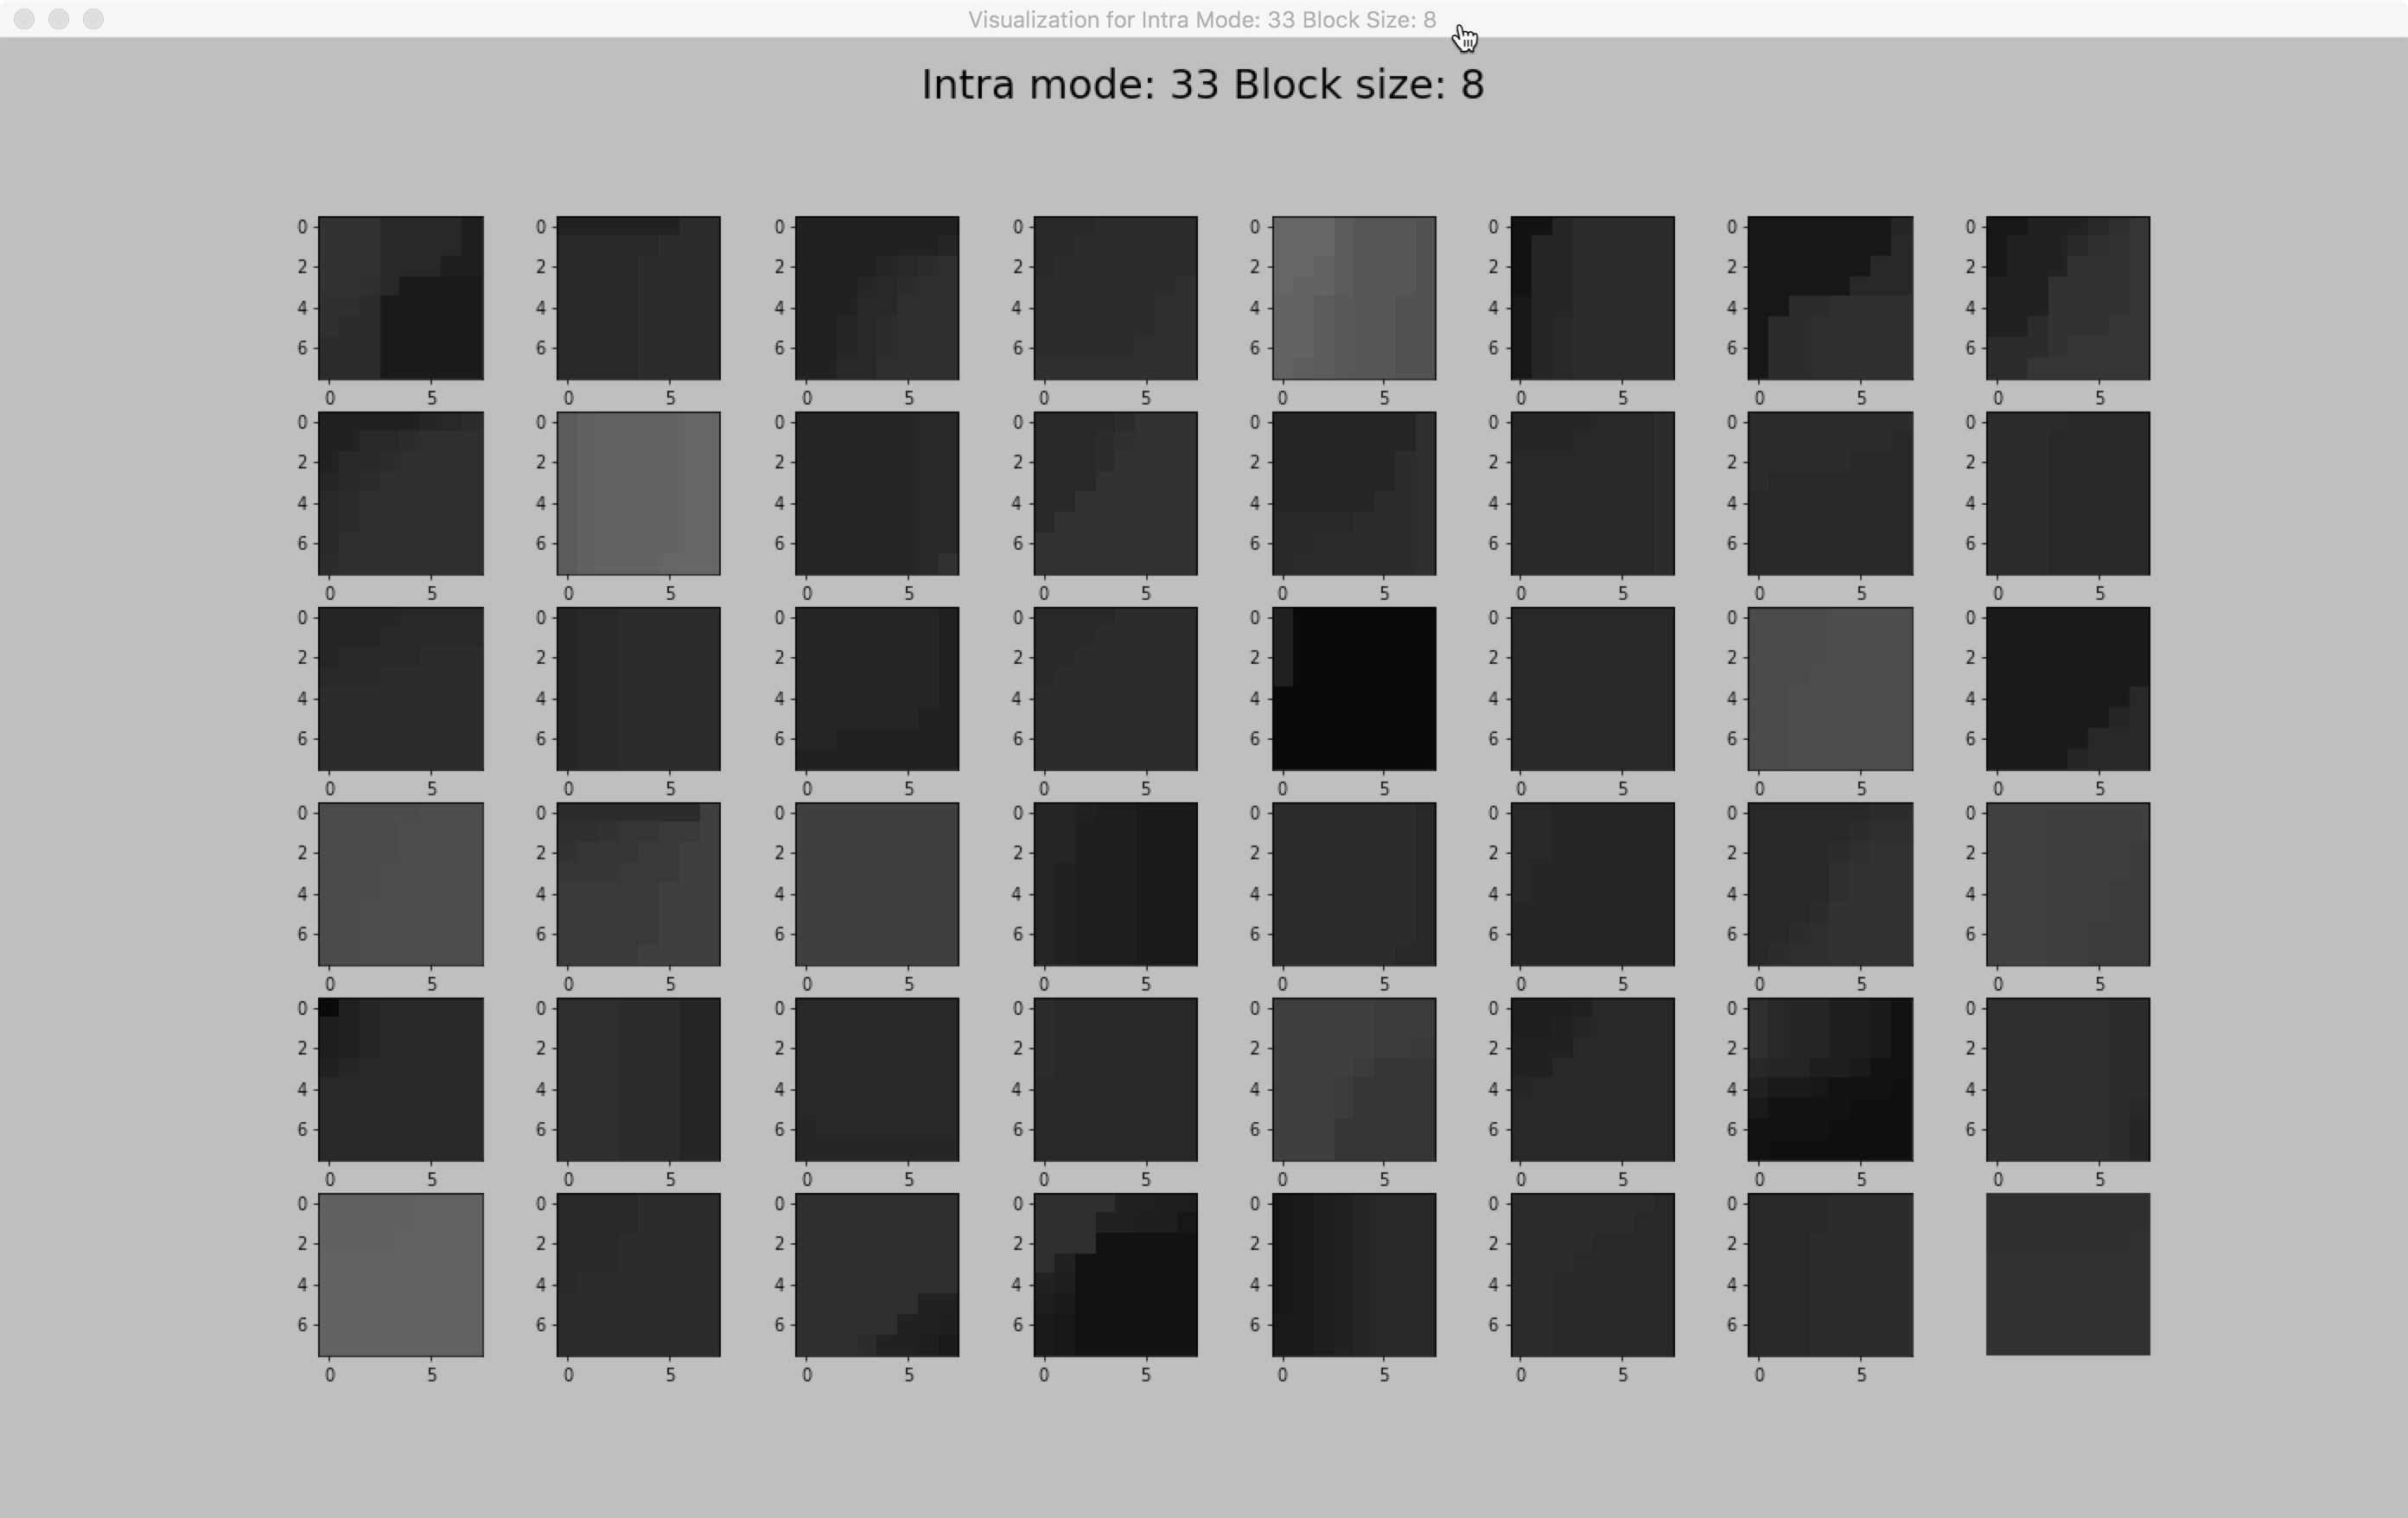
\includegraphics[width=\linewidth]{Figures/visu-size8x8/8-33}
        \caption[Intra mode 33]{intra mode 33.}
        \label{fig:size8_mode33}
    \end{minipage}
% \caption{Figure caption goes here}\label{fig:visualizations-for-blocks-of-size8x8-01}
\end{figure}
\begin{figure}[H]
    \vspace*{1cm} % vertical separation
    \begin{minipage}{0.49\textwidth}
        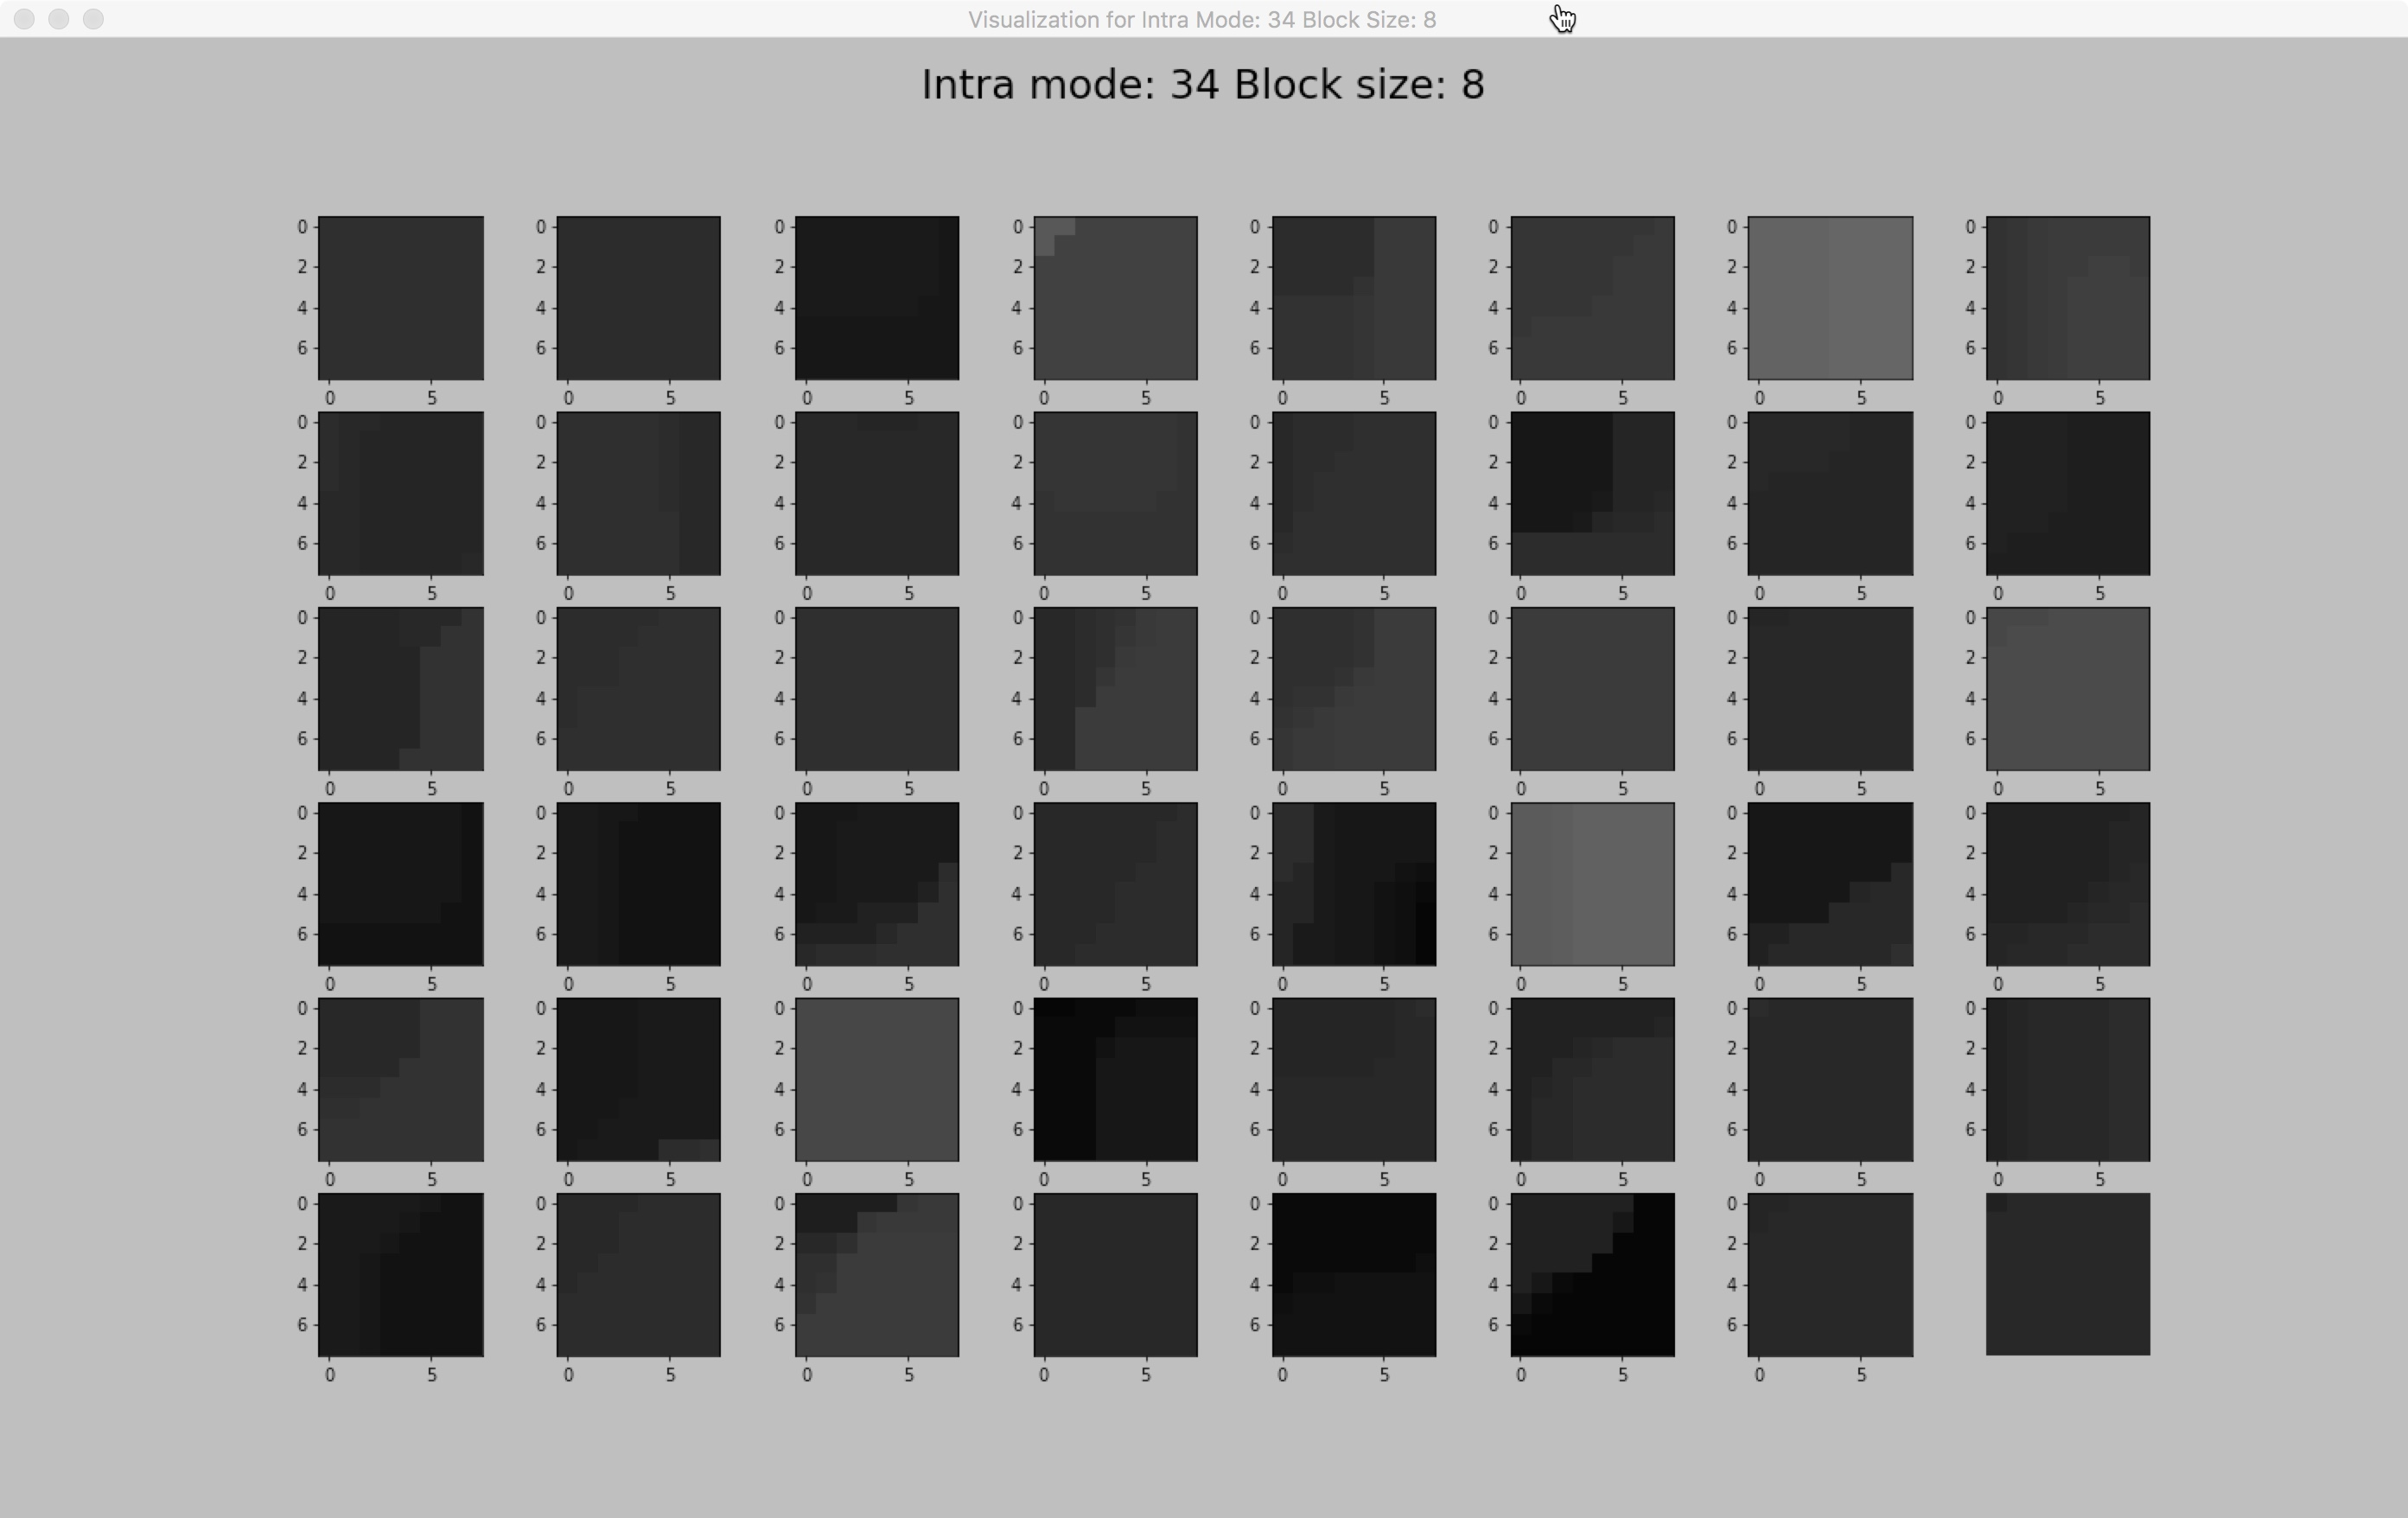
\includegraphics[width=\linewidth]{Figures/visu-size8x8/8-34}
        \caption[Intra mode 34]{intra mode 34.}
        \label{fig:size8_mode34}
    \end{minipage}
    \hspace{\fill} % note: no blank line here
    \begin{minipage}{0.49\textwidth}
        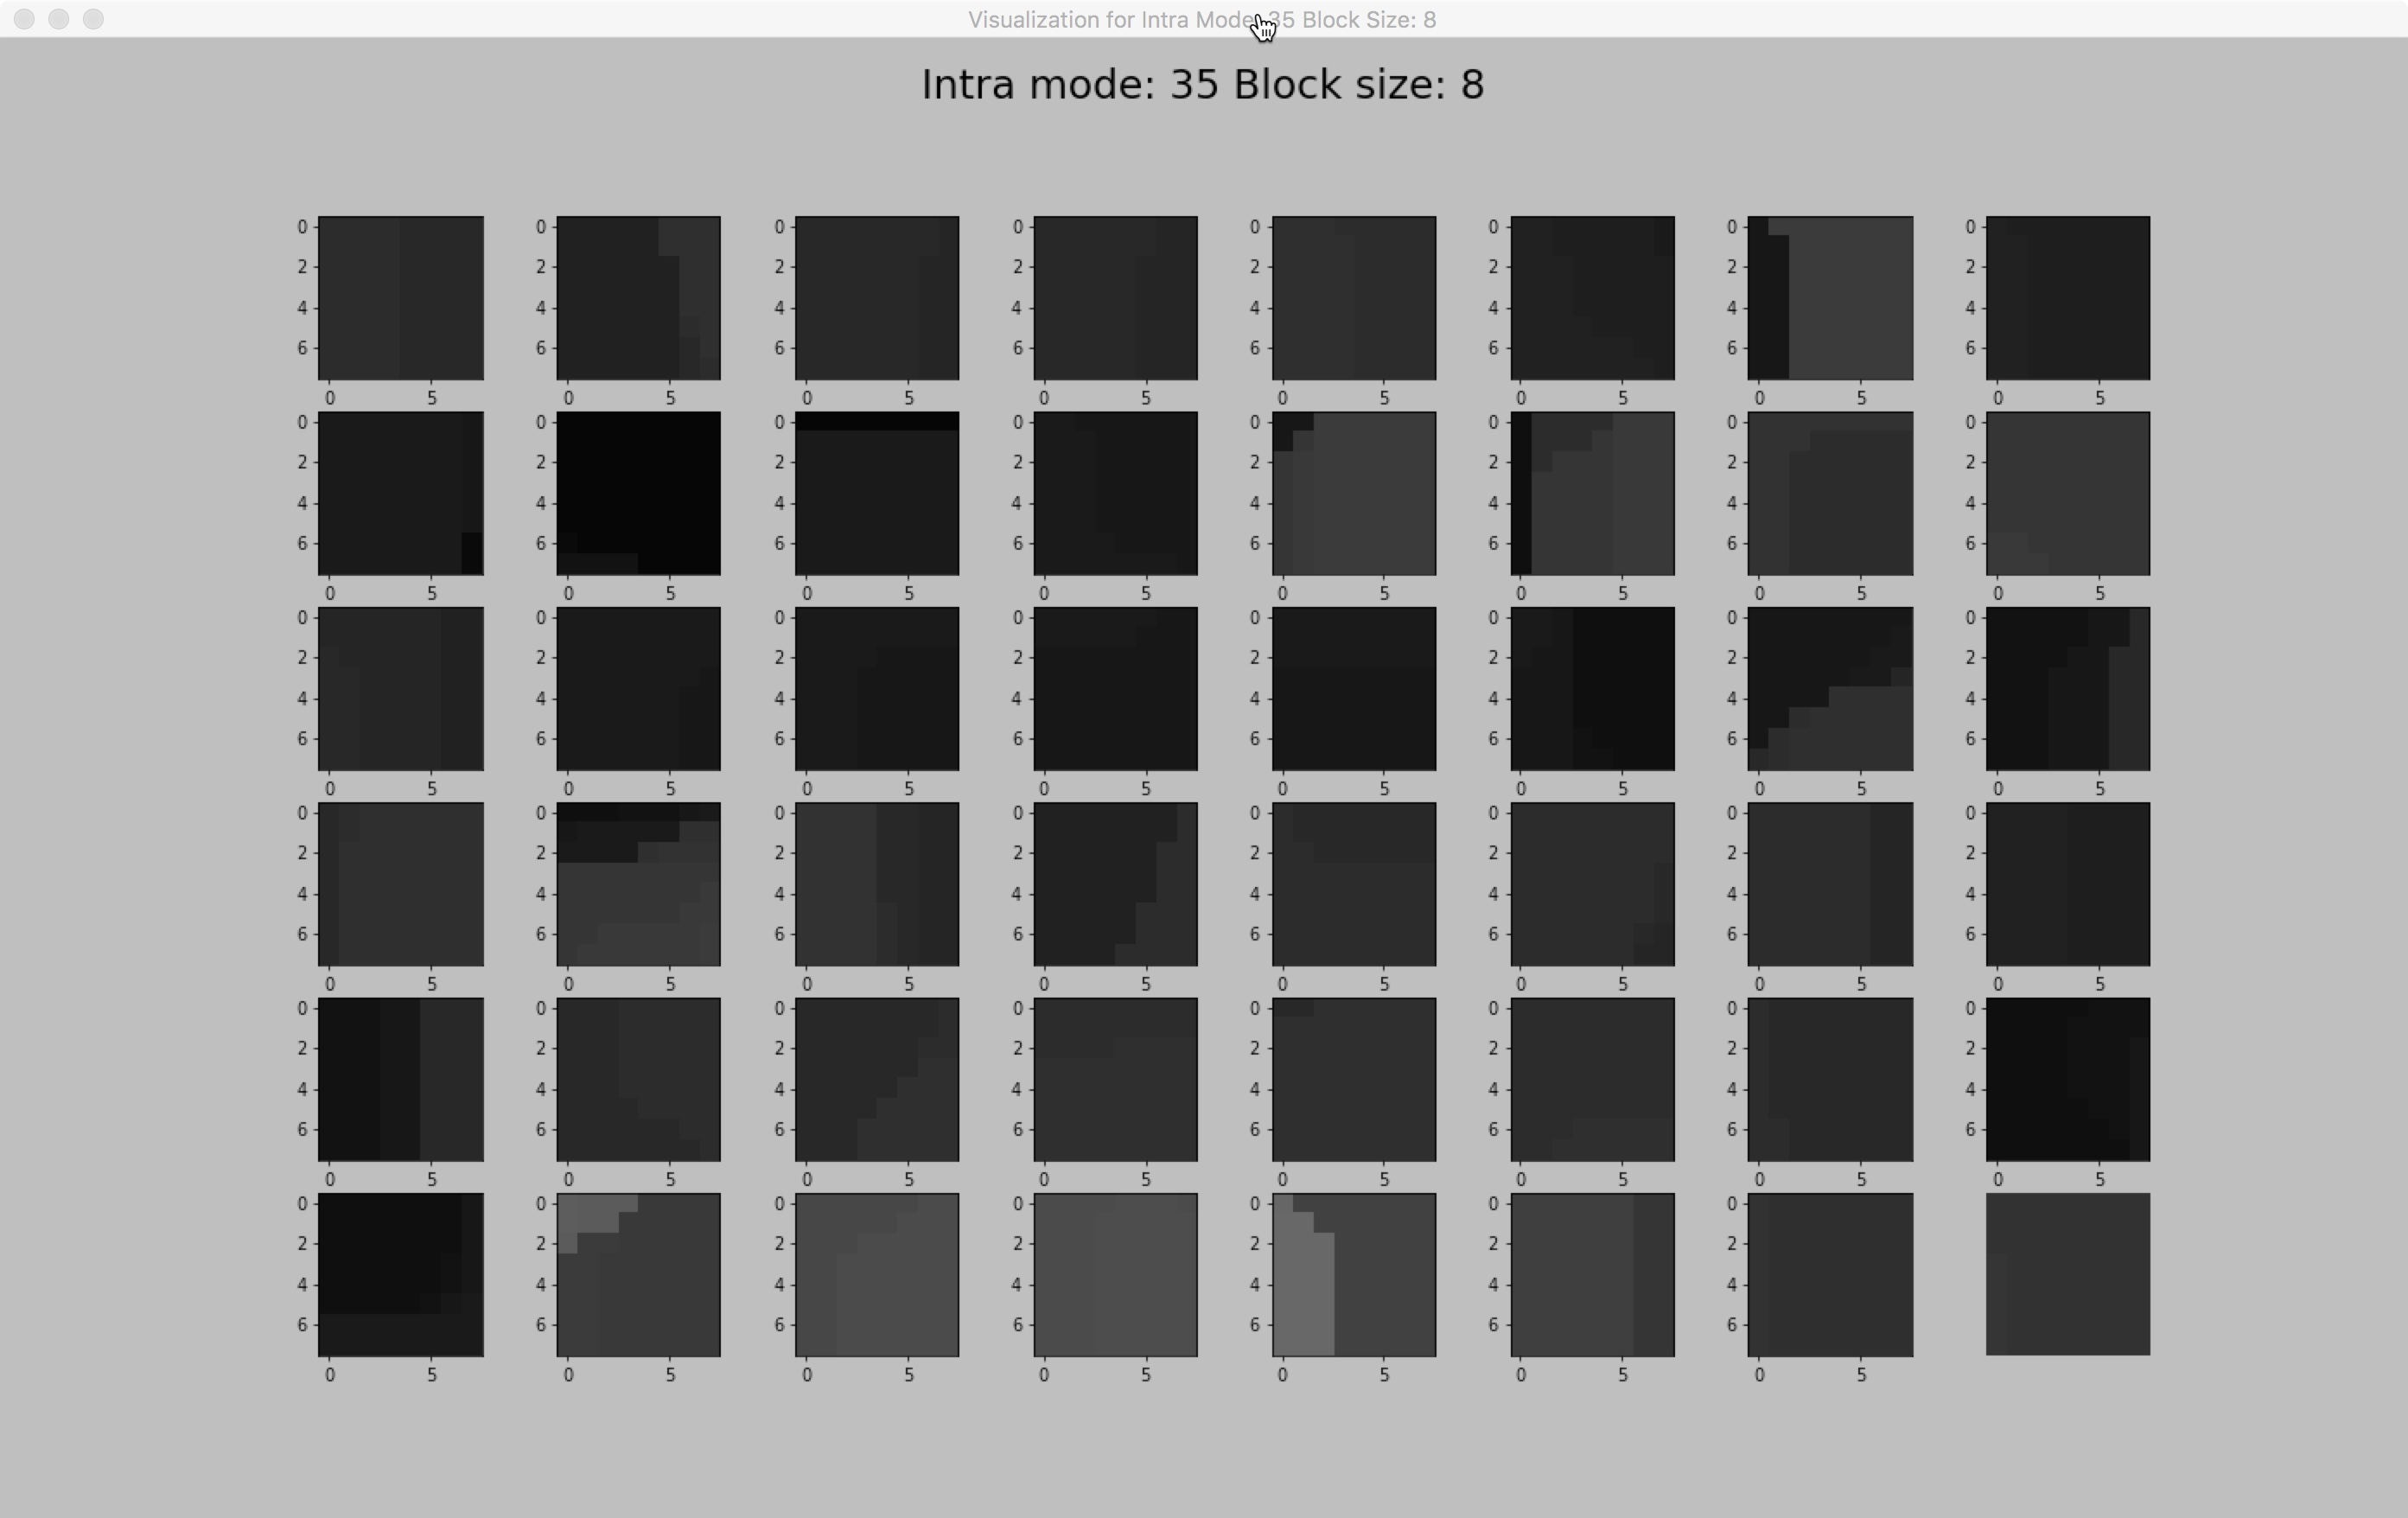
\includegraphics[width=\linewidth]{Figures/visu-size8x8/8-35}
        \caption[Intra mode 35]{intra mode 35.}
        \label{fig:size8_mode35}
    \end{minipage}
    \vspace*{1cm} % vertical separation
    \begin{minipage}{0.49\textwidth}
        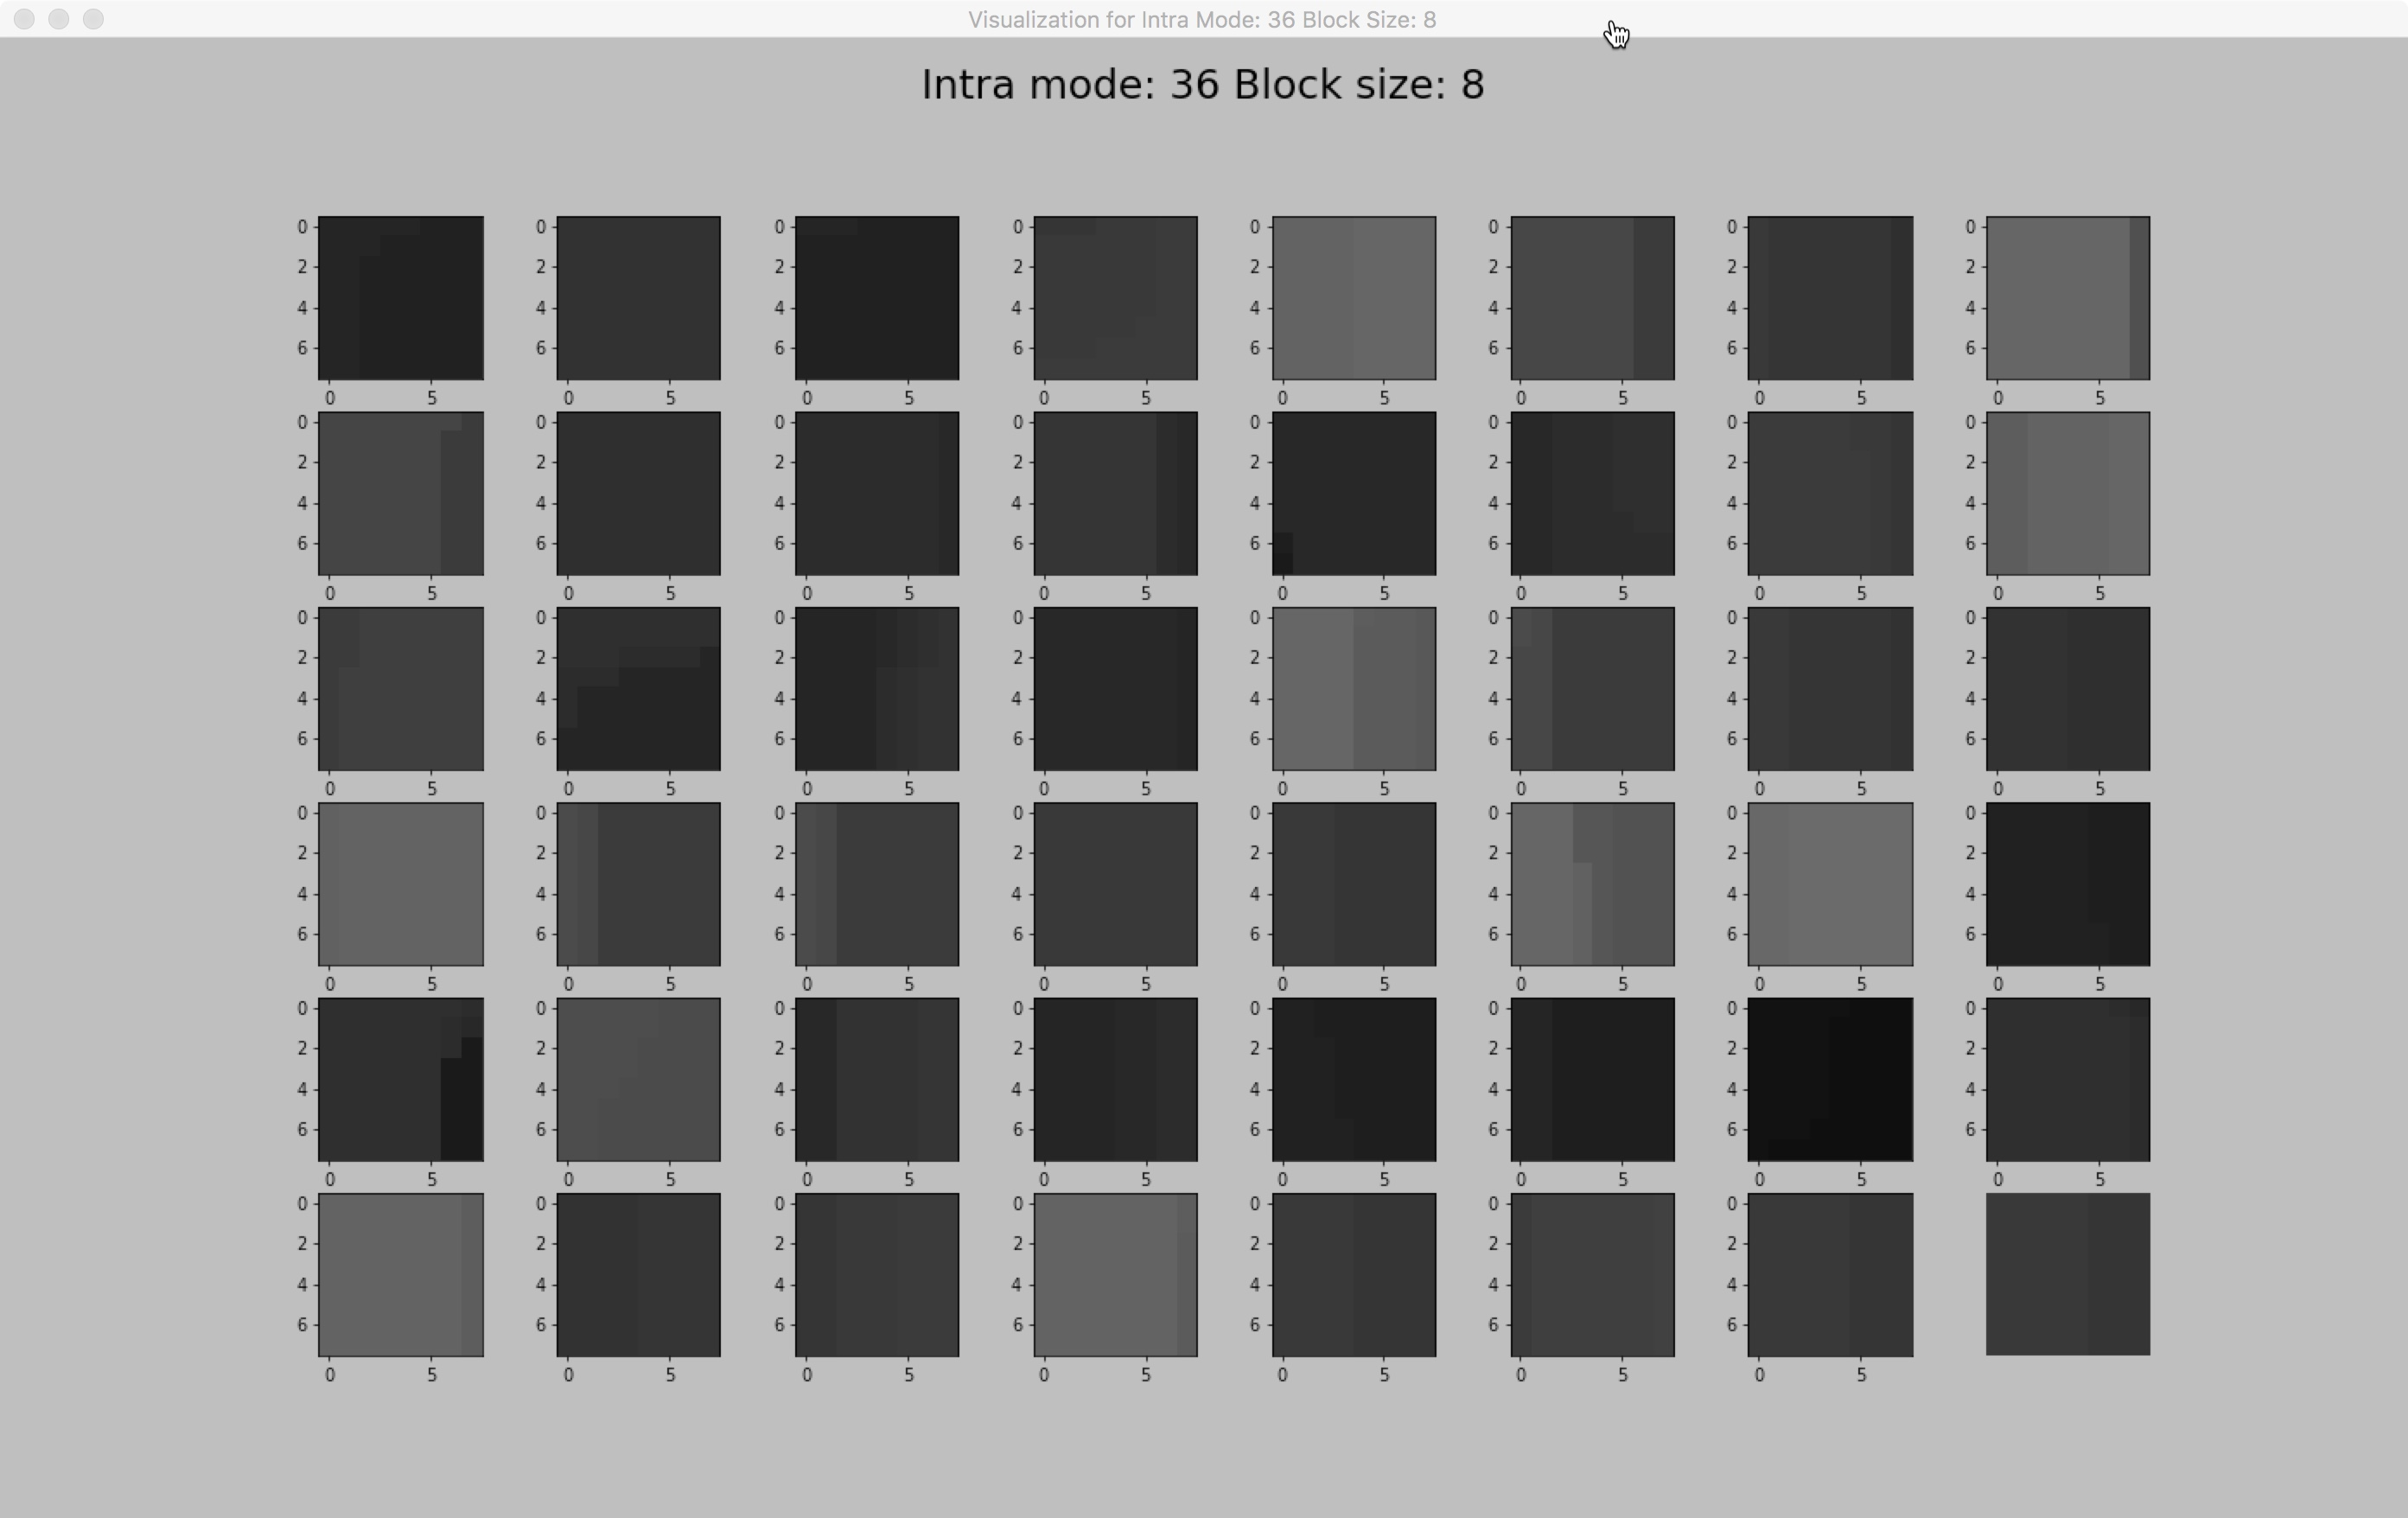
\includegraphics[width=\linewidth]{Figures/visu-size8x8/8-36}
        \caption[Intra mode 36]{intra mode 36.}
        \label{fig:size8_mode36}
    \end{minipage}
    % \caption{Figure caption goes here}\label{fig:visualizations-for-blocks-of-size8x8-01}
\end{figure}

\subsection{Discussion}\label{subsec:discussion-about-data-visu}

\section{Data Pre-processing}\label{sec:data-preprocessing}
%Welcome to this \LaTeX{} Thesis Template, a beautiful and easy to use template for writing a thesis using the \LaTeX{} typesetting system.
%
%If you are writing a thesis (or will be in the future) and its subject is technical or mathematical (though it doesn't have to be), then creating it in \LaTeX{} is highly recommended as a way to make sure you can just get down to the essential writing without having to worry over formatting or wasting time arguing with your word processor.
%
%\LaTeX{} is easily able to~\parencite{RN93} professionally typeset documents that run to hundreds or thousands of pages long. With simple mark-up commands, it automatically sets out the table of contents, margins, page headers and footers and keeps the formatting consistent and beautiful. One of its main strengths is the way it can easily typeset mathematics, even \emph{heavy} mathematics. Even if those equations are the most horribly twisted and most difficult mathematical problems that can only be solved on a super-computer, you can at least count on \LaTeX{} to make them look stunning.
%
%%----------------------------------------------------------------------------------------
%
%\section{Welcome and Thanku}\label{sec:welome}
%Welcome to this \LaTeX{} Thesis Template, a beautiful and easy to use template for writing a thesis using the \LaTeX{} typesetting system.
%
%If you are writing a thesis (or will be in the future) and its subject is technical or mathematical (though it doesn't have to be), then creating it in \LaTeX{} is highly recommended as a way to make sure you can just get down to the essential writing without having to worry over formatting or wasting time arguing with your word processor.
%
%\LaTeX{} is easily able to professionally typeset documents that run to hundreds or thousands of pages long. With simple mark-up commands, it automatically sets out the table of contents, margins, page headers and footers and keeps the formatting consistent and beautiful. One of its main strengths is the way it can easily typeset mathematics, even \emph{heavy} mathematics. Even if those equations are the most horribly twisted and most difficult mathematical problems that can only be solved on a super-computer, you can at least count on \LaTeX{} to make them look stunning.
%
%%----------------------------------------------------------------------------------------
%
%\section{Welcome and ThYou}\label{sec:weome}
%Welcome to this \LaTeX{} Thesis Template~\parencite{Reference1}, a beautiful and easy to use template for writing a thesis using the \LaTeX{} typesetting system.
%
%If you are writing a thesis (or will be in the future) and its subject is technical or mathematical (though it doesn't have to be), then creating it in \LaTeX{} is highly recommended as a way to make sure you can just get down to the essential writing without having to worry over formatting or wasting time arguing with your word processor.
%
%\LaTeX{} is easily able to professionally typeset documents that run to hundreds or thousands of pages long. With simple mark-up commands, it automatically sets out the table of contents, margins, page headers and footers and keeps the formatting consistent and beautiful. One of its main strengths is the way it can easily typeset mathematics, even \emph{heavy} mathematics. Even if those equations are the most horribly twisted and most difficult mathematical problems that can only be solved on a super-computer, you can at least count on \LaTeX{} to make them look stunning.
%
%%----------------------------------------------------------------------------------------
%
%\section{Welcome and Thau}\label{sec:welcoe}
%Welcome to this \LaTeX{} Thesis Template, a beautiful and easy to use template for writing a thesis using the \LaTeX{} typesetting system.
%
%\begin{table}
%
%    \label{tab:treatments}
%    \centering
%%    \begin{tabular}{l l l}
%%        \toprule
%%        \tabhead{Groups} & \tabhead{Treatment X} & \tabhead{Treatment Y} \\
%%        \midrule
%%        1 & 0.2 & 0.8\\
%%        2 & 0.17 & 0.7\\
%%        3 & 0.24 & 0.75\\
%%        4 & 0.68 & 0.3\\
%%        \bottomrule\\
%%    \end{tabular}
%    \begin{tabular}{c r @{.} l}
%        Pi expression       &
%        \multicolumn{2}{c}{Value} \\
%        \hline
%        $\pi$               & 3&1416  \\
%        $\pi^{\pi}$         & 36&46   \\
%        $(\pi^{\pi})^{\pi}$ & 80662&7 \\
%    \end{tabular}
%    \caption{The effects of treatments X and Y on the four groups studied.}
%\end{table}
%writing a thesis (or will be in the future) and its subject is technical or mathematical (though it doesn't have to be), then creating it in \LaTeX{} is highly recommended as a way to make sure you can just get down to the essential writing without having to worry over formatting or wasting time arguing with your word processor.
%
%\LaTeX{} is easily able to professionally typeset documents that run to hundreds or thousands of pages long. With simple mark-up commands, it automatically sets out the table of contents, margins, page headers and footers and keeps the formatting consistent and beautiful. One of its main strengths is the way it can easily typeset mathematics, even \emph{heavy} mathematics. Even if those equations are the most horribly twisted and most difficult mathematical problems that can only be solved on a super-computer, you can at least count on \LaTeX{} to make them look stunning.
%
%\section{Welcome and Tnk You}\label{sec:wlcome}
%Welcome to this \LaTeX{} Thesis Template, a beautiful and easy to use template for writing a thesis using the \LaTeX{} typesetting system.
%
%If you are writing a thesis.
%
%%\begin{verbatim}
%\begin{figure}
%    \centering
%    
\includegraphics{Figures/Electron}
%    %    \decoRule
%    \caption[An Electron]{An electron (artist's impression).}
%    \label{fig:Electron}
%\end{figure}
%%\end{verbatim}
%(or will be in the future) and its subject is technical or mathematical (though it doesn't have to be), then creating it in \LaTeX{} is highly recommended as a way to make sure you can just get down to the essential writing without having to worry over formatting or wasting time arguing with your word processor.
%
%\LaTeX{} is easily able to professionally typeset documents that run to hundreds or thousands of pages long. With simple mark-up commands, it automatically sets out the table of contents, margins, page headers and footers and keeps the formatting consistent and beautiful. One of its main strengths is the way it can easily typeset mathematics, even \emph{heavy} mathematics. Even if those equations are the most horribly twisted and most difficult mathematical problems that can only be solved on a super-computer, you can at least count on \LaTeX{} to make them look stunning.
%
%%----------------------------------------------------------------------------------------